\documentclass[titlepage]{article}

%
%  For use with latex2html
%
\usepackage{html}
\usepackage{graphics}

%
%  Set the size of the margins and text area
%
\setlength{\evensidemargin}{0.5in}
\setlength{\oddsidemargin}{0.5in}
\setlength{\textwidth}{5.5in}
\setlength{\topmargin}{0.0in}
\setlength{\headsep}{0.5in}
\setlength{\topskip}{0in}
\setlength{\marginparwidth}{1in}
\setlength{\marginparsep}{0in}
\setlength{\footskip}{0.75in}

%
%  Bring in Condor macros
%
%
%  Set up version, author and copyright notices
%
\newcommand{\AuthorNotice}{Condor Team, University of Wisconsin--Madison}
\newcommand{\VersionNotice}{Version 6.6.4}
\newcommand{\CondorR}{Condor\textsuperscript{\scriptsize{\textregistered}}}
\newcommand{\CopyrightNotice}{Copyright \copyright\ 1990-2004 Condor Team, Computer Sciences Department, 
  University of Wisconsin-Madison, Madison, WI.  All Rights Reserved.  
  No use of the Condor Software Program is authorized 
  without the express consent of the Condor Team.  For more information 
  contact: Condor Team, Attention: Professor Miron Livny, 
  7367 Computer Sciences, 1210 W. Dayton St., Madison, WI 53706-1685, 
  (608) 262-0856 or miron@cs.wisc.edu.
 
  U.S. Government Rights Restrictions: Use, duplication, or disclosure 
  by the U.S. Government is subject to restrictions as set forth in 
  subparagraph (c)(1)(ii) of The Rights in Technical Data and Computer 
  Software clause at DFARS 252.227-7013 or subparagraphs (c)(1) and 
  (2) of Commercial Computer Software-Restricted Rights at 48 CFR 
  52.227-19, as applicable, Condor Team, Attention: Professor Miron 
  Livny, 7367 Computer Sciences, 1210 W. Dayton St., Madison, 
  WI 53706-1685, (608) 262-0856 or miron@cs.wisc.edu. 

  See the \emph{Condor \VersionNotice\ Manual} for
  additional notices. }

%
%  Common motifs
%
\newcommand{\Prog}[1]{\textit{#1}}              	% Program name
\newcommand{\Term}[1]{\emph{#1}}			% Use this to introduce terminology
\newcommand{\Cmd}[2]{\textit{#1}(#2)}           	% Command w/ section number
\newcommand{\Sinful}[1]{$<$#1$>$}         	% Sinful string
\newcommand{\SinfulAny}{$<$a.b.c.d:port$>$}        	% Arbitrary Sinful string
\newcommand{\URL}[1]{\htmladdnormallink{#1}{#1}}	% a URL
\newcommand{\Email}[1]{\htmladdnormallink{#1}{mailto:#1}}
\newcommand{\File}[1]{\texttt{#1}}        	    	% File name
\newcommand{\Bs}{$\mathtt{\backslash}$}         	% Backslash
% If we don't use math mode, latex2html can use the aux files generated for
% the PDF.  Doing so also eliminates a symlink.
\newcommand{\Bar}{{\tt |}}
\newcommand{\Dots}{\dots}
	% This brings in \Bar |, \Dots ...
\newcommand{\Tilde}{\~{}}                 	% tilde
\newcommand{\Circum}{\^{}}                      	% ^
\newcommand{\Lbr}{[}                            	% [
\newcommand{\Rbr}{]}                            	% ]
\newcommand{\Percent}{\%}                       	% %
\newcommand{\Opt}[1]{\mbox{\textbf{#1}}}            % Option
\newcommand{\Arg}[1]{\mbox{\textit{#1}}}            % Argument
\newcommand{\OptArg}[2]{\mbox{\Opt{#1\ }\Arg{#2}}}  % Option with Argument
\newcommand{\oArg}[1]{\mbox{[\Arg{#1}]}}            % optional Argument
\newcommand{\oOpt}[1]{\mbox{[\Opt{#1}]}}            % optional Option
\newcommand{\oOptArg}[2]{\mbox{[\OptArg{#1\ }{#2}]}}% optional Option w/ Arg
\newcommand{\Optnm}[1]{\textbf{#1}}            % Option w/o mbox
\newcommand{\Argnm}[1]{\textit{#1}}            % Argument w/o mbox
\newcommand{\OptArgnm}[2]{\Optnm{#1\ }\Argnm{#2}}% Option with Argument w/o mbox
\newcommand{\oArgnm}[1]{[\Argnm{#1}]}            % optional Argument w/o mbox
\newcommand{\oOptnm}[1]{[\Optnm{#1}]}            % optional Option w/o mbox
\newcommand{\oOptArgnm}[2]{[\OptArgnm{#1\ }{#2}]}% optional Option w/Arg w/o mbox
\newcommand{\Env}[1]{\texttt{#1}}		% Environment variable
\newcommand{\DCPerm}[1]{\texttt{#1}}		% DC Permission
\newcommand{\ShortExpr}[1]{\mbox{\texttt{#1}}}		% A pithy config file expression
\newcommand{\Expr}[1]{\texttt{#1}}		% Config file expression
\newcommand{\MacroNI}[1]{\texttt{#1}}		% Config file macro, NO index
\newcommand{\Macro}[1]{\texttt{#1} \index{#1 macro@\texttt{#1} macro} \index{configuration macro!\texttt{#1}}}		% Config file macro and index
\newcommand{\MacroUNI}[1]{\texttt{\$(#1)}}	% Config file macro's use, NO index
\newcommand{\MacroU}[1]{\texttt{\$(#1)}\index{#1 macro@\texttt{#1} macro}\index{configuration macro!\texttt{#1}}}	% Config file macro's use and index
\newcommand{\AdAttr}[1]{\texttt{#1}}	% ClassAd Attribute name
\newcommand{\Attr}[1]{\texttt{#1}}	% ClassAd Attribute name again
\newcommand{\AdStr}[1]{\texttt{"#1"}}	% ClassAd Attribute string
\newcommand{\Dflag}[1]{\texttt{D\_#1}}		% Debug flag name
\newcommand{\Bold}[1]{\textbf{#1}}		% Something you want bold
\input{fontsize.tex}
\newcommand{\Note}{\underline{NOTE}: }          % NOTE:
\newcommand{\Warn}{\underline{WARNING}: }       % WARNING:
\newcommand{\Todo}{\begin{center} \fbox{This section has not yet been written} \end{center}}
\newcommand{\Syscall}[1]{\texttt{#1()}}		% The name of a syscall

% A keyword in a meta-language
\newcommand{\Keyword}[1] {{\tt #1}}

% The name of a procedure
\newcommand{\Procedure}[1] {{\tt #1\(\)}}

% A program code snippet
\newcommand{\Code}[1] {{\tt #1}}

% Make a nice box with a header to point out a tricky feature
\newcommand{\Notice}[1] {\noindent {\bf Notice: }\\ \fbox{\parbox[t]{\textwidth}{#1}}}

% Release directory entry
\newcommand{\Release}[1]{\texttt{$<$release\_dir$>$/#1}}


%
% This sets the BODY tag when converted to HTML.
% It has no effect on the DVI file.
\bodytext{ BGCOLOR=#FFFFFF }

%
%  To help with typing in names of condor commands
%    e.g., condor_submit == \Condor{submit}
\newcommand{\Condor}[1]{\Prog{condor\_#1}}
\newcommand{\condor}[1]{condor\_#1}



%
%  Fix the headers and footers
%
\latex{
	\usepackage{fancyhdr}
	\pagestyle{fancy}
	\fancyhf{}
	\renewcommand{\sectionmark}[1]{\markright{\thesection.\ #1}}
\if@twoside
	\fancyhead[LE,RO]{\thepage}
	\fancyhead[RE]{\leftmark}
	\fancyhead[LO]{\rightmark}
\else
	\fancyhead[R]{\thepage}
	\fancyhead[L]{\rightmark}
\fi

	\fancyfoot[C]{Condor \VersionNotice, Administrators' Manual}
	\renewcommand{\headrulewidth}{0.4pt}
	\renewcommand{\footrulewidth}{0.4pt}
	\addtolength{\headwidth}{\oddsidemargin}
}

\begin{document}

\title{Condor \VersionNotice : Administrators' Manual}
\author{\AuthorNotice}
\maketitle

\tableofcontents
\newpage

\sloppy
%
% This turns off the hbox underfull warnings, but
% does not change the formatting of the text
% default value is 1000
\hbadness=10000



\index{administrator's manual|(}

%%%%%%%%%%%%%%%%%%%%%%%%%%%%%%%%%%%%%%%%%%%%%%%%%%%%%%%%%%%%%%%%%%%%%%%%%%%
\section{\label{sec:grids-intro}An Introduction}
%%%%%%%%%%%%%%%%%%%%%%%%%%%%%%%%%%%%%%%%%%%%%%%%%%%%%%%%%%%%%%%%%%%%%%%%%%%

Grids refer to computing resources all over the world. 
Condor's purpose of providing computing cycles extends naturally
to grids.
To this end, Condor has the grid universe for jobs.
Within this universe, jobs may be specified for a variety
of grids.

An easy extension allows Condor jobs submitted within one pool
of machines to execute on another (separate) Condor pool.
Condor calls this flocking.
If a machine within the pool where a job is submitted is not
available to run the job,
the job makes its way to another pool.
This is enabled by configuration of the pools.

Some of Condor's grid computing features utilize Globus software
(\URL{http://www.globus.org/}).
Globus provides infrastructure for authentication, authorization,
and remote job submission (including data transfer) on Grid resources.
Condor-G provides all of Condor's job submission features,
but for these far-removed resources.

%%%%%%%%%%%%%%%%%%%%%%%%%%%%%%%%%%%%%%%%%%%%%%%%%%%%%%%%%%%%%%%%%%%%%%
\section{Installation of Condor}
\label{sec:install}
%%%%%%%%%%%%%%%%%%%%%%%%%%%%%%%%%%%%%%%%%%%%%%%%%%%%%%%%%%%%%%%%%%%%%%

Please refer to the \File{INSTALL} file that is included with the
Condor binary release for instructions of how to install Condor.


%%%%%%%%%%%%%%%%%%%%%%%%%%%%%%%%%%%%%%%%%%%%%%%%%%%%%%%%%%%%%%%%%%%%%%
\section{Configuring Condor}
\label{sec:Configuring-Condor}
%%%%%%%%%%%%%%%%%%%%%%%%%%%%%%%%%%%%%%%%%%%%%%%%%%%%%%%%%%%%%%%%%%%%%%

This section describes how to configure all parts of the Condor
system.  First, we describe some general information about the config
files, their syntax, etc.  Then, we describe settings that effect all
Condor daemons and tools.  Finally, we have a section describing the
settings for each part of Condor.  The only exception to this are the
settings that control the policy under which Condor will start,
suspend, resume, vacate or kill jobs.  These settings (and other
important concepts from the \Condor{startd}) are described in 
section~\ref{sec:Configuring-Policy} on ``Configuring Condor's Job
Execution Policy''. 

%%%%%%%%%%%%%%%%%%%%%%%%%%%%%%%%%%%%%%%%%%%%%%%%%%%%%%%%%%%%%%%%%%%%%%
\subsection{Introduction to Config Files}
\label{sec:Intro-to-Config-Files}
%%%%%%%%%%%%%%%%%%%%%%%%%%%%%%%%%%%%%%%%%%%%%%%%%%%%%%%%%%%%%%%%%%%%%%

The Condor configuration files are used to customize how Condor
operates at a given site.  The basic configuration as shipped with
Condor should work well for most sites, with a few exceptions of
things that might need special customization.  Please see the section
from the Installation section of this manual for details on where
Condor's config files are found.

Each condor program will, as part of its initialization process,
``configure'' itself by calling a library routine which parses the
various config files that might be used including pool-wide,
machine-specific, and root-owner config files.  The result is a list
of constants and expressions which the program may evaluate as needed
at run time.

Definitions in the configuration file come in two flavors, macros and
expressions.  Macros provide string valued constants which remain
static throughout the execution of the program.  Expressions can be
arithmetic, boolean, or string valued, and can be evaluated
dynamically at run time.


%%%%%%%%%%%%%%%%%%%%%%%%%%%%%%%%%%%%%%%%%%%%%%%%%%%%%%%%%%%%%%%%%%%%%%
\subsubsection{Config File Macros}
\label{sec:Config-File-Macros}
%%%%%%%%%%%%%%%%%%%%%%%%%%%%%%%%%%%%%%%%%%%%%%%%%%%%%%%%%%%%%%%%%%%%%%

Macro definitions are of the form:

\begin{verbatim}
        <macro_name> = <macro_definition>
\end{verbatim}

\textbf{NOTE:} You must have whitespace between the macro name, the
``='' sign, and the macro definition.  Macro invocations are of the
form: 

\begin{verbatim}
        $(macro_name)
\end{verbatim}

Macro definitions may contain references to \textbf{previously defined
  macros}.  Nothing in a config file can reference Macros which have
  not yet been defined.  Thus,

\begin{verbatim}
        A = xxx
        C = $(A) 
\end{verbatim}

is a legal set of macro definitions, and the resulting value of ``C'' is
``xxx''.  Note that ``C'' is actually bound to ``\MacroU{A}'', not its value, thus

\begin{verbatim}
        A = xxx
        C = $(A)
        A = yyy
\end{verbatim}

is also a legal set of macro definitions and the resulting value of
``C'' is ``yyy''.  However, 

\begin{verbatim}
        A = $(C)
        C = xxx
\end{verbatim}

is not legal, and will result in the Condor daemons and tools exiting
when they try to parse their config files.

%%%%%%%%%%%%%%%%%%%%%%%%%%%%%%%%%%%%%%%%%%%%%%%%%%%%%%%%%%%%%%%%%%%%%%
\subsubsection{Config File Expressions}
\label{sec:Config-File-Expressions}
%%%%%%%%%%%%%%%%%%%%%%%%%%%%%%%%%%%%%%%%%%%%%%%%%%%%%%%%%%%%%%%%%%%%%%

Expression definitions are of the form:

\begin{verbatim}
        <expression_name> : <expression>
\end{verbatim}

\textbf{NOTE:} You must have whitespace between the expression name,
the ``:'' sign, and the expression definition.  Expressions may
contain constants, operators, and other expressions.  Macros may also
be used to aid in writing expressions.  Constants may be booleans,
denoted by ``true'' (or ``t'') or ``false'' (or ``f''), signed
integers, floating point values, or strings enclosed in double quotes
(").  All config file expressions are simply inserted into various
ClassAds.  Please see the appendix on ClassAds for details about
ClassAd expression operators, and how ClassAd expressions are
evaluated.

Note that expression which contain references to other expressions are
bound to the expressions definition, not its current value, but
functions which contain macro invocations are bound to the current
value of the macro.  Thus

\begin{verbatim}
        X : "xxx"
        Y : X
        X : "yyy"
\end{verbatim}

will result in ``Y'' being evaluated as ``yyy'' at run time, but

\begin{verbatim}
        X = "xxx"
        Y : $(X)
        X = "yyy" 
\end{verbatim}

will result in ``Y'' having a run time value of ``xxx''.

%%%%%%%%%%%%%%%%%%%%%%%%%%%%%%%%%%%%%%%%%%%%%%%%%%%%%%%%%%%%%%%%%%%%%%
\subsubsection{Other Syntax}
\label{sec:Other-Syntax}
%%%%%%%%%%%%%%%%%%%%%%%%%%%%%%%%%%%%%%%%%%%%%%%%%%%%%%%%%%%%%%%%%%%%%%

Other than macros and expressions, a Condor config file can contain
comments or continuations.  A comment is any line begining with a
``\#''.  A continuation is any entry (either macro or expression) that
continues across multiples lines.  This is accomplished with the
``\\'' sign at the end of any line that you wish to continue onto
another.  For example,

\begin{verbatim}
        START : (KeyboardIdle > 15 * $(MINUTE)) && \
                ((LoadAvg - CondorLoadAvg) <= 0.3)
\end{verbatim}

or,

\begin{verbatim}
        ADMIN_MACHINES = condor.cs.wisc.edu, raven.cs.wisc.edu, \
                        stork.cs.wisc.edu, ostrich.cs.wisc.edu, \
                        bigbird.cs.wisc.edu
        HOSTALLOW_ADMIN = $(ADMIN_MACHINES)
\end{verbatim}

%%%%%%%%%%%%%%%%%%%%%%%%%%%%%%%%%%%%%%%%%%%%%%%%%%%%%%%%%%%%%%%%%%%%%%
\subsubsection{Pre-Defined Macros and Expressions}
\label{sec:Pre-Defined-Macros-and-Expressions}
%%%%%%%%%%%%%%%%%%%%%%%%%%%%%%%%%%%%%%%%%%%%%%%%%%%%%%%%%%%%%%%%%%%%%%

Condor provides a number of pre-defined macros and expressions that
help you configure Condor.  Pre-defined macros are listed as
\MacroU{macro\_name}, while pre-defined expressions are just listed as
\Expr{expression\_name}, to denote how they should be referenced in
other macros or expressions.

The first set are special entries whose values are determined at
runtime and cannot be overridden.  These are inserted automatically by
the library routine which parses the config files.

\begin{description}
  
\item[\Expr{CurrentTime}] \label{param:CurrentTime} This expression
  provides the current result of the system call \Cmd{time}{2}.  This
  is an integer containing the number of seconds since an arbitrary
  date defined by UNIX as the ``beginning of time'', hereafter
  referred to as the \Term{UNIX date}.
  
\item[\MacroU{full\_hostname}] \label{param:FullHostname} This is the
  fully qualified hostname of the local machine (hostname plus domain
  name).
  
\item[\MacroU{hostname}] \label{param:Hostname} This is just the
  hostname of the local machine (no domain name).
  
\item[\MacroU{tilde}] \label{param:Tilde} This is the full path to the
  home directory of user ``condor'', if such a user exists on the
  local machine.

\end{description}

%%%%%%%%%%%%%%%%%%%%%%%%%%%%%%%%%%%%%%%%%%%%%%%%%%%%%%%%%%%%%%%%%%%%%%
\subsubsection{Condor Subsystem Names}
\label{sec:Condor-Subsystem-Names}
%%%%%%%%%%%%%%%%%%%%%%%%%%%%%%%%%%%%%%%%%%%%%%%%%%%%%%%%%%%%%%%%%%%%%%

\textbf{IMPORTANT NOTE:} Many of the entries in the config file will
be named with the \Term{subsystem} of the various Condor daemons.
This is a unique string which identifies a given daemon within the
Condor system.  The possible subsystem names are:

\begin{itemize}
\item STARTD
\item SCHEDD
\item MASTER
\item COLLECTOR
\item NEGOTIATOR
\item KBDD 
\item SHADOW
\item STARTER
\item CKPT\_SERVER
\label{list:subsystem names}
\end{itemize}

In the description of the actual config file entries, ``SUBSYS'' will
stand for one of these possible subsystem names.

%%%%%%%%%%%%%%%%%%%%%%%%%%%%%%%%%%%%%%%%%%%%%%%%%%%%%%%%%%%%%%%%%%%%%%
\subsection{Condor-wide Config File Entries}
\label{sec:Condor-wide-Config-File-Entries}
%%%%%%%%%%%%%%%%%%%%%%%%%%%%%%%%%%%%%%%%%%%%%%%%%%%%%%%%%%%%%%%%%%%%%%
This section describes settings which effect all parts of the Condor
system. 

\begin{description}
  
\item[\Macro{CONDOR\_HOST}] \label{param:CondorHost} This macro is
  just used to define the \Macro{NEGOTIATOR\_HOST} and
  \Macro{COLLECTOR\_HOST} macros.  Normally, the \Condor{collector}
  and \Condor{negotiator} would run on the same machine.  If for some
  reason they weren't, \Macro{CONDOR\_HOST} would not be needed.  Some
  of the host-based security macros use \Macro{CONDOR\_HOST} by
  default.  See section~\ref{sec:Host-Security} on ``Setting up
  IP/host-based security in Condor'' for details.
  
\item[\Macro{COLLECTOR\_HOST}] \label{param:CollectorHost} The
  hostname of the machine where the \Condor{collector} is running for
  your pool.  Normally it would just be defined with the
  \Macro{CONDOR\_HOST} macro described above.

\item[\Macro{NEGOTIATOR\_HOST}] \label{param:NegotiatorHost} The
  hostname of the machine where the \Condor{negotiator} is running for
  your pool.  Normally it would just be defined with the
  \Macro{CONDOR\_HOST} macro described above.

\item[\Macro{RELEASE\_DIR}] \label{param:ReleaseDir} The full path to
  the Condor release directory, which holds the bin, etc, lib, and
  sbin directories.  Other macros are defined relative to this one.

\item[\Macro{BIN}] \label{param:Bin} This directory points to the
  Condor bin directory, where user-level programs are installed.  It
  is usually just defined relative to the \Macro{RELEASE\_DIR} macro.
  
\item[\Macro{LIB}] \label{param:Lib} This directory points to the
  Condor lib directory, where libraries used to link jobs for Condor's
  standard universe are stored.  The \Condor{compile} program uses
  this macro to find these libraries, so it must be defined.
  \Macro{LIB} is usually just defined relative to the
  \Macro{RELEASE\_DIR} macro.

\item[\Macro{SBIN}] \label{param:Sbin} This directory points to the
  Condor sbin directory, where Condor's system binaries (such as the
  binaries for the Condor daemons) and administrative tools are
  installed.  Whatever directory \Macro{SBIN} points to should
  probably be in the \Env{PATH} of anyone who is acting as a Condor
  administrator.

\item[\Macro{LOCAL\_DIR}] \label{param:LocalDir} The location of the
  local Condor directory on each machine in your pool.  One common
  option is to use the condor user's home directory which you could
  specify with \MacroU{tilde}.  For example:

\begin{verbatim}
        LOCAL_DIR = $(tilde)
\end{verbatim}
  
  On machines with a shared filesystem, where either the
  \MacroU{tilde} directory or another directory you want to use is
  shared among all machines in your pool, you might use the
  \MacroU{hostname} macro and have a directory with many
  subdirectories, one for each machine in your pool, each named by
  hostnames.  For example:

\begin{verbatim}
        LOCAL_DIR = $(tilde)/hosts/$(hostname)      
\end{verbatim}

  or:

\begin{verbatim}
        LOCAL_DIR = $(release_dir)/hosts/$(hostname)
\end{verbatim}

  
\item[\Macro{LOG}] \label{param:Log} This entry is used to specify the
  directory where each Condor daemon writes its log files.  The names
  of the log files themselves are defined with other macros, which use
  the \Macro{LOG} macro by default.  The log directory also acts as
  the current working directory of the Condor daemons as the run, so
  if one of them should drop a core file for any reason, it would wind
  up in the directory defined by this macro.  Normally, \Macro{LOG} is
  just defined in terms of \MacroU{LOCAL\_DIR}.
  
\item[\Macro{SPOOL}] \label{param:Spool} The spool directory is where
  certain files used by the \Condor{schedd} are stored, such as the
  job queue file, and the initial executables of any jobs that have
  been submitted.  In addition, if you are not using a checkpoint
  server, all the checkpoint files from jobs that have been submitted
  from a given machine will be store in that machine's spool
  directory.  Therefore, you will want to ensure that the spool
  directory is located on a partition with enough disk space.  If a
  given machine is only setup to execute Condor jobs and not submit
  them, it would not need a spool directory (or this macro defined).
  Normally, \Macro{SPOOL} is just defined in terms of
  \MacroU{LOCAL\_DIR}.
  
\item[\Macro{EXECUTE}] \label{param:Execute} This directory acts as
  the current working directory of any Condor job that is executing on
  the local machine.  If a given machine is only setup to only submit
  jobs and not execute them, it would not need an execute directory
  (or this macro defined).  Normally, \Macro{EXECUTE} is just defined
  in terms of \MacroU{LOCAL\_DIR}.
  
\item[\Macro{LOCAL\_CONFIG\_FILE}] \label{param:LocalConfigFile} The
  location of the local, machine-specific config file for each machine
  in your pool.  The two most common options would be putting this
  file in the \MacroU{LOCAL\_DIR} you just defined, or putting all
  local config files for your pool in a shared directory, each one
  named by hostname.  For example:

\begin{verbatim}
        LOCAL_CONFIG_FILE = $(LOCAL_DIR)/condor_config.local
\end{verbatim}
  
  or:

\begin{verbatim}
        LOCAL_CONFIG_FILE = $(release_dir)/etc/$(hostname).local
\end{verbatim}
  
  or, not using your release directory:

\begin{verbatim}
        LOCAL_CONFIG_FILE = /full/path/to/configs/$(hostname).local
\end{verbatim}
  
\item[\Macro{CONDOR\_ADMIN}] \label{param:CondorAdmin} This is the email
  address that Condor will send mail to when something goes wrong in
  your pool.  For example, if a daemon crashes, the \Condor{master}
  can send an \Term{obituary} to this address with the last few lines
  of that daemon's log file and a brief message that describes what
  signal or exit status that daemon exited with.
  
\item[\Macro{MAIL}] \label{param:Mail} This is the full path to a mail
  sending program that understands that ``-s'' means you wish to
  specify a subject to the message you're sending.  On all platforms,
  the default shipped with Condor should work.  Only if you have
  installed things in a non-standard location on your system would you
  need to change this setting.
  
\item[\Macro{RESERVED\_SWAP}] \label{param:ReservedSwap} This setting
  determines how much swap space you want to reserve for your own
  machine.  Condor will not start up more \Condor{shadow} processes if
  the amount of free swap space on your machine falls below this
  level. 

\item[\Macro{RESERVED\_DISK}] \label{param:ReservedDisk} This setting
  determines how much disk space you want to reserve for your own
  machine.  When Condor is reporting the amount of free disk space in
  a given partition on your machine, it will always subtract this
  amount.  For example, the \Condor{startd} advertises the amount of
  free space in the \Macro{EXECUTE} directory described above.
  
\item[\Macro{ARCH}] \label{param:Arch} This setting defines the string
  used to identify the architecture of the local machine to Condor.
  The \Condor{startd} will advertise itself with this attribute so
  that users can submit binaries compiled for a given platform and
  force them to run on the correct machines.  \Condor{submit} will
  automatically append a requirement to the job ClassAd that it must
  run on the same \Macro{ARCH} and \Macro{OPSYS} of the machine where
  it was submitted, unless the user specifies \Macro{ARCH} and/or
  \Macro{OPSYS} explicitly in their submit file.  The the
  \Cmd{\condor{submit}}{1} man page for details.  If this setting is
  not defined in the config file, Condor will automatically insert the
  architecture of this machine as determined by \Prog{uname -m}
  (machine).

\item[\Macro{OPSYS}] \label{param:OpSys} This settings defines the
  string used to identify the operating system of the local machine to
  Condor.  See the entry on \Macro{ARCH} above for more information.
  If this setting is not defined in the config file, Condor will
  automatically insert the operating system of this machine as
  determined by the concatenation of \Prog{uname -s} and \Prog{uname
    -r} (system and release).
  
\item[\Macro{LOCK}] \label{param:Lock} Condor needs to create a few
  lock files to synchronize access to various log files.  Because of
  problems we've had with network filesystems and file locking over
  the years, we \textbf{highly} recommend that you put these lock
  files on a local partition on each machine.  If you don't have your
  \Macro{LOCAL\_DIR} on a local partition, be sure to change this
  entry.  Whatever user (or group) condor is running as needs to have
  write access to this directory.  If you're not running as root, this
  is whatever user you started up the \Condor{master} as.  If you are
  running as root, and there's a condor account, it's probably condor.
  Otherwise, it's whatever you've set in the \Env{CONDOR\_IDS}
  environment variable.  See section~\ref{sec:uids} on ``UIDs in
  Condor'' for details on this.

\item[\Macro{HISTORY}] \label{param:History} This entry defines the
  location of the Condor history file, which stores information about
  all Condor jobs that have completed on a given machine.  This entry
  is used by both the \Condor{schedd} which appends the information,
  and \Condor{history}, the user-level program that is used to view
  the history file.

\end{description}


%%%%%%%%%%%%%%%%%%%%%%%%%%%%%%%%%%%%%%%%%%%%%%%%%%%%%%%%%%%%%%%%%%%%%%%%%%%
\subsection{Daemon Logging Config File Entries}
\label{sec:Daemon-Logging-Config-File-Entries}
%%%%%%%%%%%%%%%%%%%%%%%%%%%%%%%%%%%%%%%%%%%%%%%%%%%%%%%%%%%%%%%%%%%%%%%%%%%

These entries control how and where the Condor daemons write their log
files.  All of these entries are named with the subsystem (as
described in section~\ref{sec:Condor-Subsystem-Names} above) of the daemon
you wish to control logging for.

\begin{description}
 
\item[\Macro{SUBSYS\_LOG}] \label{param:SubsysLog} This is the name of
  the log file for the given subsystem.  For example,
  \Macro{STARTD\_LOG} gives the location of the log file for the
  \Condor{startd}.  These entries are defined relative to the
  \Macro{LOG} macro described above.  The actual names of the files
  are also used in the \Macro{VALID\_LOG\_FILES} entry used by
  \Condor{preen}, which is described below.  If you change one of the
  filenames with this setting, be sure to change the
  \Macro{VALID\_LOG\_FILES} entry as well, or \Condor{preen} will
  delete your newly named log files.  
  
\item[\Macro{MAX\_SUBSYS\_LOG}] \label{param:MaxSubsysLog} This
  setting controls the maximum length in bytes to which the various
  logs will be allowed to grow.  Each log file will grow to the
  specified length, then be saved to a ``.old'' file.  The ``.old''
  files are overwritten each time the log is saved, thus the maximum
  space devoted to logging for any one program will be twice the
  maximum length of its log file.

\item[\Macro{TRUNC\_SUBSYS\_LOG\_ON\_OPEN}]
  \label{param:TruncSubsysLogOnOpen}  If this macro is defined and set
  to ``True'' the affected log will be truncated and started from an
  empty file with each invocation of the program.  Otherwise, new
  invocations of the program will simply append to the previous log
  file.  By default this setting is turned off for all daemons. 

\item[\Macro{SUBSYS\_DEBUG}] \label{param:SubsysDebug} All of the
  Condor daemons can produce different levels of output depending on
  how much information you want to see.  The various levels of
  verbosity for a given daemon are determined by this entry.  All
  daemons have a default level, \Dflag{ALWAYS}, and log message for
  that level will be printed to the daemon's log, regardless of what
  you have set here.  The other possible debug levels are:

\begin{description}
  
\item[\Dflag{FULLDEBUG}] \label{dflag:fulldebug} Generally, turning on
  this setting provides very verbose output in the log files.

\item[\Dflag{DAEMONCORE}] \label{dflag:daemoncore} This provides log
  file entries for things that are specific to DaemonCore, such as
  timers the daemons have set, the commands that are registered, and
  so on.  If both \Dflag{FULLDEBUG} and \Dflag{DAEMONCORE} are set,
  you get \textbf{VERY} verbose output.

\item[\Dflag{PRIV}] \label{dflag:priv} This flag provides turns on log
  messages about the \Term{privilege state} switching that the daemons
  do.  See section~\ref{sec:uids} on UIDs in Condor for more details.

\item[\Dflag{COMMAND}] \label{dflag:command} With this flag set, a
  Any daemon that uses DaemonCore will print out a log message
  whenever a command comes in.  The name and integer of the command
  are printed, whether the command was sent via UDP or TCP, and where
  the command was sent from.  Because the \Condor{kbdd} works by
  sending UDP commands to the \Condor{startd} whenever there is
  activity on the X server, we don't recommend turning on
  \Dflag{COMMAND} login in the \Condor{startd}, since you will get so
  many messages that the log file will be fairly useless to you.  On
  platforms that use the \Condor{kbdd}, this is turned off in the
  \Condor{startd} by default.

\item[\Dflag{LOAD}] \label{dflag:load} The \Condor{startd} keeps track
  of the load average on the machine where it is running.  Both the
  general system load average, and the load average being generated by
  Condor's activity there.  With this flag set, the \Condor{startd}
  will print out a log message with the current state of both of these
  load averages whenever it computes them.  This flag only effects the
  \Condor{startd}.
  
\item[\Dflag{JOB}] \label{dflag:job} When this flag is set, the
  \Condor{startd} will dump out to its log file the contents of any
  job ClassAd that the \Condor{schedd} sends to claim the
  \Condor{startd} for its use.  This flag only effects the
  \Condor{startd}.
  
\item[\Dflag{MACHINE}] \label{dflag:machine} When this flag is set,
  the \Condor{startd} will dump out to its log file the contents of
  its resource ClassAd when the \Condor{schedd} tries to claim the
  \Condor{startd} for its use.  This flag only effects the
  \Condor{startd}.

\item[\Dflag{SYSCALLS}] \label{dflag:syscalls} This flag is used to
  make the \Condor{shadow} log remote syscall requests and return
  values.  This can help track down problems a user is having with a
  particular job since you can see what system calls the job is
  performing, which, if any, are failing, and what the reason for the
  failure is.  The \Condor{schedd} also uses this flag for the server
  portion of the queue management code.  So, with \Dflag{SYSCALLS}
  defined in \Macro{SCHEDD\_DEBUG} you will see verbose logging of all
  queue management operations the \Condor{schedd} performs.  

\label{list:debug level description}
\end{description}

\end{description}

%%%%%%%%%%%%%%%%%%%%%%%%%%%%%%%%%%%%%%%%%%%%%%%%%%%%%%%%%%%%%%%%%%%%%%%%%%%
\subsection{DaemonCore Config File Entries}
\label{sec:DaemonCore-Config-File-Entries}
%%%%%%%%%%%%%%%%%%%%%%%%%%%%%%%%%%%%%%%%%%%%%%%%%%%%%%%%%%%%%%%%%%%%%%%%%%%

Please read section~\ref{sec:DaemonCore} on ``DaemonCore'' for details
about DaemonCore is.  There are certain config file settings that
DaemonCore uses which affect all Condor daemons (except the checkpoint
server, shadow, and starter, none of which use DaemonCore yet).

\begin{description}
  
\item[\Macro{HOSTALLOW\Dots}] \label{param:HostAllow} All of the
  settings that begin with either \Macro{HOSTALLOW} or
  \Macro{HOSTDENY} are settings for Condor's host-based security.
  Please see section~\ref{sec:Host-Security} on ``Setting up
  IP/host-based security in Condor'' for details on all of these
  settings and how to configure them.

\item[\Macro{SHUTDOWN\_GRACEFUL\_TIMEOUT}]
  \label{param:ShutdownGracefulTimeout} This entry determines how long
  you are willing to let daemons try their graceful shutdown methods
  before they do a hard shutdown.  It is defined in terms of seconds.
  The default is 1800 (30 minutes).

\item[\Macro{SUBSYS\_ADDRESS\_FILE}]
  \label{param:SubsysAddressFile} Every Condor daemon that uses
  DaemonCore has a command port where commands can be sent.  The
  IP/port of the daemon is put in that daemon's ClassAd so that other
  machines in the pool can query the \Condor{collector} (which listens
  on a well-known port) to find the address of a given daemon on a
  given machine.  However, tools and daemons executing on the same
  machine they wish to communicate with don't have to query the
  collector, they can simply look in a file on the local disk to find
  the IP/port.  Setting this entry will cause daemons to write the
  IP/port of their command socket to the file you specify.  This way,
  local tools will continue to operate, even if the machine running
  the \Condor{collector} crashes.  Using this file will also generate
  slightly less network traffic in your pool (since \Condor{q},
  \Condor{rm}, etc won't have to send any messages over the network to
  locate the \Condor{schedd}, for example).  This entry is not needed
  for the collector or negotiator, since their command sockets are at
  well-known ports anyway.  
  
\item[\Macro{SUBSYS\_EXPRS}] \label{param:SubsysExprs} This entry
  allows you to have the any DaemonCore daemon advertise arbitrary
  expressions from the config file in its ClassAd.  Give the
  comma-separated list of entries from the config file you want in the
  given daemon's ClassAd.
  
  \textbf{NOTE:} The \Condor{negotiator} and \Condor{kbdd} do not send
  ClassAds now, so this entry does not effect them at all.  The
  \Condor{startd}, \Condor{schedd}, \Condor{master}, and
  \Condor{collector} do send ClassAds, so those would be valid
  subsystems to set this entry for.
  
  \textbf{OTHER NOTE:} Because of the different syntax of the config
  file and ClassAds, you might have to do a little extra work to get a
  given entry into the ClassAd.  In particular, ClassAds require quote
  marks (") around your strings.  Numeric values can go in directly,
  as can expressions or boolean macros.  For example, if you wanted
  the startd to advertise a macro that was a string, a numeric macro,
  and a boolean expression, you'd have to do something like the
  following:

\begin{verbatim}
        STRING_MACRO = This is a string macro
        NUMBER_MACRO = 666
        BOOL_MACRO = True
        EXPR : CurrentTime >= $(NUMBER_MACRO) || $(BOOL_MACRO)
        MY_STRING_MACRO = "$(STRING_MACRO)"
        STARTD_EXPRS = MY_STRING_MACRO, NUMBER_MACRO, BOOL_MACRO, EXPR
\end{verbatim}

\end{description}

%%%%%%%%%%%%%%%%%%%%%%%%%%%%%%%%%%%%%%%%%%%%%%%%%%%%%%%%%%%%%%%%%%%%%%%%%%%
\subsection{Shared Filesystem Config File Entries}
\label{sec:Shared-Filesystem-Config-File-Entries}
%%%%%%%%%%%%%%%%%%%%%%%%%%%%%%%%%%%%%%%%%%%%%%%%%%%%%%%%%%%%%%%%%%%%%%%%%%%

These entries control how Condor interacts with various shared and
network filesystems.  If you are using AFS as your shared filesystem,
be sure to read section~\ref{sec:Condor-AFS} on ``Using Condor with
AFS''

\begin{description}

\item[\Macro{UID\_DOMAIN}] \label{param:UidDomain} Often times,
  especially if all the machines in the pool are administered by the
  same organization, all the machines to be added into a Condor pool
  share the same login account information.  Specifically, does user X
  have UID Y on all machines within a given Internet/DNS domain? This
  is usually the case if a central authority creates user logins and
  maintains a common /etc/passwd file on all machines (perhaps via
  NIS/Yellow Pages, distributing the passwd file, etc). If this is the
  case, then set this macro to the name of the Internet/DNS domain
  where this is true. For instance, if all the machines in this Condor
  pool within the Internet/DNS zone ``cs.wisc.edu'' have a common
  passwd file, \Macro{UID\_DOMAIN} would be set to ``cs.wisc.edu''. If
  this is not the case you can comment out the entry and Condor will
  automatically use the fully qualified hostname of each machine.  If
  you put in a ``*'', that means a wildcard to match all domains and
  therefore to honor all UIDs - dangerous idea.
          
  Condor uses this information to determine if it should run a given
  Condor job on the remote execute machine with the UID of whomever
  submitted the job or with the UID of user ``nobody''.  If you set
  this to ``none'' or don't set it at all, then Condor jobs will
  always execute with the access permissions of user ``nobody''.  For
  security purposes, it is not a bad idea to have Condor jobs that
  migrate around on machines across an entire organization to run as
  user ``nobody'', which by convention has very restricted access to
  the disk files of a machine.  Standard Universe Condor jobs are
  perfectly happy to run as user nobody since all I/O is redirected
  back via remote system calls to a shadow process running on the
  submit machine which is authenticated as the user.  If you only plan
  on running Standard Universe jobs, then it is a good idea to simply
  set this to ``none'' or don't define it.  Vanilla Universe jobs,
  however, cannot take advantage of Condor's remote system calls.
  Vanilla Universe jobs are dependent upon NFS, RFS, AFS, or some
  shared filesystem setup to read/write files as they bounce around
  from machine to machine. If you want to run Vanilla jobs and your
  shared filesystems are via AFS, then you can safely leave this as
  ``none'' as well. But if you wish to use Vanilla jobs with Condor
  and you have shared filesystems via NFS or RFS, then you should
  enter in a legitimate domain name where all your UIDs match (you
  should be doing this with NFS anyway!) on all machines in the pool,
  or else users in your pool who submit Vanilla jobs will have to make
  their files world read/write (so that user nobody can access them).
          
  Some gritty details for folks who want to know: If the submitting
  machine and the remote machine about to execute the job both have
  the same login name in the passwd file for a given UID, and the
  \Macro{UID\_DOMAIN} claimed by the submit machine is indeed found to
  be a subset of what an inverse lookup to a DNS (domain name server)
  reports as the fully qualified domain name for the submit machine's
  IP address (this security measure safeguards against the submit
  machine from simply lying), \textbf{THEN} the job will run with the
  same UID as the user who submitted the job.  Otherwise it will run
  as user ``nobody''.
          
  Note: the \Macro{UID\_DOMAIN} parameter is also used when Condor
  sends email back to the user about a completed job; the address
  \texttt{Job-Owner@UID\_DOMAIN} is used, unless \Macro{UID\_DOMAIN}
  is ``none'', in which case \texttt{Job-Owner@submit-machine} is
  used.
  
\item[\Macro{FILESYSTEM\_DOMAIN}] \label{param:FilesystemDomain} This
  setting is similar in concept to \Macro{UID\_DOMAIN}, but here we
  need the Internet/DNS domain name where all the machines within that
  domain can access the same set of NFS file servers.  
          
  Often times, especially if all the machines in the pool are
  administered by the same organization, all the machines to be added
  into a Condor pool can mount the same set of NFS fileservers onto
  the same place in the directory tree.  Specifically, do all the
  machines in the pool within a specific Internet/DNS domain mount the
  same set of NFS file servers onto the same path mount-points?  If
  this is the case, then set this macro to the name of the
  Internet/DNS domain where this is true.  For instance, if all the
  machines in the Condor pool within the Internet/DNS zone
  ``cs.wisc.edu'' have a common passwd file and mount the same volumes
  from the same NFS servers, set \Macro{FILESYSTEM\_DOMAIN} to
  ``cs.wisc.edu''.  If this is not the case you can comment out the
  entry, and Condor will automatically set it to the fully qualified
  hostname of the local machine.
  
\item[\Macro{HAS\_AFS}] \label{param:HasAfs} Set this to ``True'' if
  all the machines you plan on adding in your pool all can access a
  common set of AFS fileservers.  Otherwise, set it to ``False''.
      
\item[\Macro{FS\_PATHNAME}] \label{param:FsPathname} If you're using
  AFS, Condor needs to know where the AFS ``fs'' command is located so
  that it can verify the AFS cell-names of machines in the pool.  The
  default value of \File{/usr/afsws/bin/fs} is also the default that
  AFS uses.
  
\item[\Macro{VOS\_PATHNAME}] \label{param:VosPathname} If you're using
  AFS, Condor needs to know where the AFS ``vos'' command is located
  so that it can compare fileserver names of volumes.  The default
  value of \File{/usr/afsws/etc/vos} is also the default that AFS
  uses. 

\item[\Macro{RESERVE\_AFS\_CACHE}] \label{param:ReserveAfsCache} If
  your machine is running AFS and the AFS cache lives on the same
  partition as the other Condor directories, and you want Condor to
  reserve the space that your AFS cache is configured to use, set this
  entry to ``True''.  It defaults to ``False''.
  
\item[\Macro{USE\_NFS}] \label{param:UseNfs} This setting influences
  how Condor jobs running in the Standard Universe will access their
  files.  Condor will normally always redirect the file I/O requests
  of Standard Universe jobs back to be executed on the machine which
  submitted the job.  Because of this, as a Condor job migrates around
  the network, the filesystem always appears to be identical to the
  filesystem where the job was submitted.  However, consider the case
  where a user's data files are sitting on an NFS server. The machine
  running the user's program will send all I/O over the network to the
  machine which submitted the job, which in turn sends all the I/O
  over the network a second time back to the NFS file server. Thus,
  all of the program's I/O is being sent over the network twice.
          
  If you set this macro to ``True'', then Condor will attempt to
  read/write files without redirecting them back to the submitting
  machine if both the submitting machine and the machine running the
  job are both accessing the same NFS servers (if they're both in the
  same \Macro{FILESYSTEM\_DOMAIN}, as described above).  The result is
  I/O performed by Condor Standard Universe programs is only sent over
  the network once.  
          
  While sending all file operations over the network twice might sound
  really bad, unless you are operating over networks where bandwidth
  as at a very high premium, practical experience reveals that this
  scheme offers very little real performance gain.  There are also
  some (fairly rare) situations where this scheme can break down.
  
  Setting \Macro{USE\_NFS} to ``False'' is always safe.  It may result
  in slightly more network traffic, but Condor jobs are ideally heavy
  on CPU and light on I/O anyway.  It also ensures that a remote
  Standard Universe Condor job will always use Condor's remote system
  calls mechanism to reroute I/O and therefore see the exact same
  filesystem that the user sees on the machine where she/he submitted
  the job.
  
  Some gritty details for folks who want to know: If the you set
  \Macro{USE\_NFS} to ``True'', and the \Macro{FILESYSTEM\_DOMAIN} of
  both the submitting machine and the remote machine about to execute
  the job match, and the \Macro{FILESYSTEM\_DOMAIN} claimed by the
  submit machine is indeed found to be a subset of what an inverse
  lookup to a DNS (domain name server) reports as the fully qualified
  domain name for the submit machine's IP address (this security
  measure safeguards against the submit machine from simply lying),
  \textbf{THEN} the job will access files via a local system call,
  without redirecting them to the submitting machine (a.k.a. with
  NFS).  Otherwise, the system call will get routed back to the
  submitting machine via Condor's remote system call mechanism.
  
\item[\Macro{USE\_AFS}] \label{param:UseAfs} If your machines have AFS
  and the submit and execute machines are in the same AFS cell, this
  setting determines whether Condor will use remote system calls for
  Standard Universe jobs to send I/O requests to the submit machine,
  or if it should use local file access on the execute machine (which
  will then use AFS to get to the submitter's files).  Read the
  setting above on \Macro{USE\_NFS} for a discussion of why you might
  want to use AFS access instead of remote system calls.
  
  One important difference between \Macro{USE\_NFS} and
  \Macro{USE\_AFS} is the AFS cache.  With \Macro{USE\_AFS} set to
  ``True'', the remote Condor job executing on some machine will start
  messing with the AFS cache, possibly evicting the machine owner's
  files from the cache to make room for its own.  Generally speaking,
  since we try to minimize the impact of having a Condor job run on a
  given machine, we don't recomend using this setting.

  While sending all file operations over the network twice might sound
  really bad, unless you are operating over networks where bandwidth
  as at a very high premium, practical experience reveals that this
  scheme offers very little real performance gain.  There are also
  some (fairly rare) situations where this scheme can break down.
  
  Setting \Macro{USE\_AFS} to ``False'' is always safe.  It may result
  in slightly more network traffic, but Condor jobs are ideally heavy
  on CPU and light on I/O anyway.  ``False'' ensures that a remote
  Standard Universe Condor job will always see the exact same
  filesystem that the user on sees on the machine where he/she
  submitted the job.  Plus, it will ensure that the machine where the
  job executes doesn't have its AFS cache screwed up as a result of
  the Condor job being there.  
  
  However, things may be different at your site, which is why the
  setting is there.

\end{description}

%%%%%%%%%%%%%%%%%%%%%%%%%%%%%%%%%%%%%%%%%%%%%%%%%%%%%%%%%%%%%%%%%%%%%%%%%%%
\subsection{Checkpoint Server Config File Entries}
\label{sec:Checkpoint-Server-Config-File-Entries}
%%%%%%%%%%%%%%%%%%%%%%%%%%%%%%%%%%%%%%%%%%%%%%%%%%%%%%%%%%%%%%%%%%%%%%%%%%%

These entries control whether or not Condor user a checkpoint server.
In addition, if you are using a checkpoint server, this section
describes the settings that the checkpoint server itself needs to have
defined.  If you decide to use a checkpoint server, you must install
it seperately (it is not included in the main Condor binary
distribution or installation procedure).  See
section~\ref{sec:Ckpt-Server} on ``Installing a Checkpoint Server''
for details on installing and running a checkpoint server for your
pool.

\textbf{NOTE:} If you are setting up a machine to join to UW-Madison CS
Department Condor pool, you \textbf{should} configure the machine to
use a checkpoint server, and use ``condor-ckpt.cs.wisc.edu'' as the
checkpoint server host (see below).

\begin{description}
  
\item[\Macro{USE\_CKPT\_SERVER}] \label{param:UseCkptServer} A boolean
  which determines if you want a given machine machine to use the
  checkpoint server for your pool.  

\item[\Macro{CKPT\_SERVER\_HOST}] \label{param:CkptServerHost} The
  hostname of the checkpoint server for your pool.  
  
\item[\Macro{CKPT\_SERVER\_DIR}] \label{param:CkptServerDir} The
  checkpoint server needs this macro defined to the full path of the
  directory the server should use to store checkpoint files.
  Depending on the size of your pool and the size of the jobs your
  users are submitting, this directory (and it's subdirectories) might
  need to store many megabytes of data.

\end{description}


%%%%%%%%%%%%%%%%%%%%%%%%%%%%%%%%%%%%%%%%%%%%%%%%%%%%%%%%%%%%%%%%%%%%%%%%%%%
\subsection{\condor{master} Config File Entries}
\label{sec:Master-Config-File-Entries}
%%%%%%%%%%%%%%%%%%%%%%%%%%%%%%%%%%%%%%%%%%%%%%%%%%%%%%%%%%%%%%%%%%%%%%%%%%%

These settings control the \Condor{master}.

\begin{description}
  
\item[\Macro{DAEMON\_LIST}] \label{param:DaemonList} This macro
  determines what daemons the \Condor{master} will start and keep its
  watchful eyes on.  The list is a comma or space seperated list of
  subsystem names (described above in
  section~\ref{sec:Condor-Subsystem-Names}).  For example,

\begin{verbatim}
        DAEMON_LIST = MASTER, STARTD, SCHEDD
\end{verbatim}

  \textbf{NOTE:} On your central manager, your \Macro{DAEMON\_LIST}
  will be different from your regular pool, since it will include
  entries for the \Condor{collector} and \Condor{negotiator}.  
  
  \textbf{NOTE:} On machines running Digital Unix or IRIX, your
  \Macro{DAEMON\_LIST} will also include ``KBDD'', for the
  \Condor{kbdd}, which is a special daemon that runs to monitor
  keyboard and mouse activity on the console.  It is only with this
  special daemon that we can aquire this information on those
  platforms. 

\item[\Macro{SUBSYS}] \label{param:SUBSYS} Once you have defined which
  subsystems you want the \Condor{master} to start, you must provide
  it with the full path to each of these binaries.  For example:

\begin{verbatim}
        MASTER          = $(SBIN)/condor_master
        STARTD          = $(SBIN)/condor_startd
        SCHEDD          = $(SBIN)/condor_schedd
\end{verbatim}

  Generally speaking, these would be defined relative to the
  \Macro{SBIN} macro.
  
\item[\Macro{PREEN}] \label{param:Preen} In addition to the daemons
  defined in \Macro{DAEMON\_LIST}, the \Condor{master} also starts up
  a special process, \Condor{preen} to clean out junk files that have
  been left lying around by Condor.  This macro determines where the
  \Condor{master} finds the preen binary.  It also controls how
  \Condor{preen} behaves by the command-line arguments you pass to
  ``-m'' means you want email about files \Condor{preen} finds that it
  thinks it should remove.  ``-r'' means you want \Condor{preen} to
  actually remove these files.  If you don't want preen to run at all,
  just comment out this setting.

\item[\Macro{PREEN\_INTERVAL}] \label{param:PreenInterval} This macro
  determines how often \Condor{preen} should be started.  It is
  defined in terms of seconds and defaults to 86400 (once a day).

\item[\Macro{PUBLISH\_OBITUARIES}] \label{param:PublishObituaries}
  When a daemon crashes, the \Condor{master} can send email to the
  address specified by \Macro{CONDOR\_ADMIN} with an obituary letting
  the administrator know that the daemon died, what it's cause of
  death was (which signal or exit status it exited with), and
  (optionally) the last few entries from that daemon's log file.  If
  you want these obituaries, set this entry to ``True''.

\item[\Macro{OBITUARY\_LOG\_LENGTH}] \label{param:ObituaryLogLength}
  If you're getting obituaries, this setting controls how many lines
  of the log file you want to see.

\item[\Macro{START\_MASTER}] \label{param:StartMaster} If this setting
  is defined and set to ``False'' when the master starts up, the first
  thing it will do is exit.  This may seem strange, but perhaps you
  just don't want Condor to run on certain machines in your pool, yet
  the boot scripts for your entire pool are handled by a centralized
  system that starts up the \Condor{master} automatically.  This is
  certainly an entry you'd most likely find in a local config file,
  not your global config file.

\item[\Macro{START\_DAEMONS}] \label{param:StartDaemons} This setting
  is similar to the \Macro{START\_MASTER} macro described above.
  However, the \Condor{master} doesn't exit, it just doesn't start any
  of the daemons listed in the \Macro{DAEMON\_LIST}.  This way, you
  could start up the daemons at some later time with a \Condor{on}
  command if you wished.

\item[\Macro{MASTER\_UPDATE\_INTERVAL}]
  \label{param:MasterUpdateInterval} This entry determines how often
  the \Condor{master} sends a ClassAd update to the
  \Condor{collector}.  It is defined in seconds and defaults to 300
  (every 5 minutes).
  
\item[\Macro{MASTER\_CHECK\_NEW\_EXEC\_INTERVAL}]
  \label{param:MasterCheckNewExecInterval} This
  setting controls how often the \Condor{master} checks the timestamps
  of the daemons it's running.  If any daemons have been modified, the
  master restarts them.  It is defined in seconds and defaults to 300
  (every 5 minutes).

\item[\Macro{MASTER\_NEW\_BINARY\_DELAY}]
  \label{param:MasterNewBinaryDelay} Once the \Condor{master} has
  discovered a new binary, this macro controls how long it waits
  before attempting to execute the new binary.  This delay is here
  because the \Condor{master} might notice a new binary while you're
  in the process of copying in new binaries and the entire file might
  not be there yet (in which case trying to execute it could yield
  unpredictable results).  The entry is defined in seconds and
  defaults to 120 (2 minutes).

\item[\Macro{SHUTDOWN\_FAST\_TIMEOUT}]
  \label{param:ShutdownFastTimeout} This macro determines the maximum
  amount of time you're willing to give the daemons to perform their
  fast shutdown procedure before the \Condor{master} just kills them
  outright.  It is defined in seconds and defaults to 120 (2 minutes).

\item[\Macro{MASTER\_BACKOFF\_FACTOR}]
  \label{param:MasterBackoffFactor} If a daemon keeps crashing, we
  use \Term{exponential backoff} so we wait longer and longer before
  restarting it.  At the end of this section, there is an example that
  shows how all these settings work.  This setting is the base of the
  exponent used to determine how long to wait before starting the
  daemon again.  It defaults to 2.

\item[\Macro{MASTER\_BACKOFF\_CEILING}]
  \label{param:MasterBackoffCeiling} This entry determines the maximum
  amount of time you want the master to wait between attempts to start
  a given daemon.  (With 2.0 as the \Macro{MASTER\_BACKOFF\_FACTOR},
  you'd hit 1 hour in 12 restarts).  This is defined in terms of
  seconds and defaults to 3600 (1 hour).

\item[\Macro{MASTER\_RECOVER\_FACTOR}]
  \label{param:MasterRecoverFactor}  How long should a daemon run
  without crashing before we consider it \Term{recovered}.  Once a
  daemon has recovered, we reset the number of restarts so the
  exponential backoff stuff goes back to normal.  This is defined in
  terms of seconds and defaults to 300 (5 minutes).

\end{description}

Just for clarity, here's a little example of how all these exponential
backoff settings work.  The example is worked out in terms of the
default settings.

When a daemon crashes, it is restarted in 10 seconds.  If it keeps
crashing, we wait longer and longer before restarting it based on how
many times it's been restarted.  We take the number of times the
daemon has restarted, take the \Macro{MASTER\_BACKOFF\_FACTOR}
(defaults to 2) to that power, and add 9.  Sounds complicated, but
here's how it works:

\begin{verbatim}
        1st crash:  restarts == 0, so, 9 + 2^0 = 9 + 1 = 10 seconds
        2nd crash:  restarts == 1, so, 9 + 2^1 = 9 + 2 = 11 seconds
        3rd crash:  restarts == 2, so, 9 + 2^2 = 9 + 4 = 13 seconds
        ...
        6th crash:  restarts == 5, so, 9 + 2^5 = 9 + 32 = 41 seconds
        ...
        9th crash:  restarts == 8, so, 9 + 2^8 = 9 + 256 = 265 seconds
\end{verbatim}

If the daemon kept dying and restarting, after the 13th crash, you'd
have:

\begin{verbatim}
        13th crash:  restarts == 12, so, 9 + 2^12 = 9 + 4096 = 4105 seconds
\end{verbatim}

This is bigger than the \Macro{MASTER\_BACKOFF\_CEILING}, which
defaults to 3600, so the daemon would really be restarted after only
3600 seconds, not 4105.  Assuming a few hours went by like this, with
the \Condor{master} trying again every hour (since the numbers would
get even more huge, but would always be capped by the ceiling).
Eventually, imagine that daemon finally started and didn't crash (for
example, after the email you got about the daemon crashing, you
realized that you had accidentally deleted its binary so you
reinstalled it).  If it stayed alive for
\Macro{MASTER\_RECOVER\_FACTOR} seconds (defaults to 5 minutes).  We'd
reset the count of how many restarts this daemon has performed.  So,
if 15 minutes later, it died again, it would be restarted in 10
seconds, not 1 hour.

The moral of the story is that this is some relatively complicated
stuff.  The defaults we have work quite well, and you probably 
won't want to change them for any reason.


%%%%%%%%%%%%%%%%%%%%%%%%%%%%%%%%%%%%%%%%%%%%%%%%%%%%%%%%%%%%%%%%%%%%%%%%%%%
\subsection{\condor{startd} Config File Entries}
\label{sec:Startd-Config-File-Entries}
%%%%%%%%%%%%%%%%%%%%%%%%%%%%%%%%%%%%%%%%%%%%%%%%%%%%%%%%%%%%%%%%%%%%%%%%%%%

These settings control general operation of the \Condor{startd}.
Information on how to configure the \Condor{startd} to start, suspend,
resume, vacate and kill remote Condor jobs can be found in a separate
top-level section, section~\ref{sec:Configuring-Policy} on
``Configuring The Startd Policy''.  In there, you will find
information on the startd's \Term{states} and \Term{activities}.  If
you see entries in the config file that are not described here, it is
because they control state or activity transitions within the
\Condor{startd} and are described in
section`\ref{sec:Configuring-Policy}. 

\begin{description}

\item[\Macro{STARTER}] \label{param:Starter}  This macro holds the full
  path to the regular \Condor{starter} binary the startd should
  spawn.  It is normally defined relative to \MacroU{SBIN}.
  
\item[\Macro{ALTERNATE\_STARTER\_1}] \label{param:AlternateStarter1}
  This macro holds the full path to the special \Condor{starter.pvm}
  binary the startd spawns to service PVM jobs.  It is normally
  defined relative to \MacroU{SBIN}, since by default,
  \Condor{starter.pvm} is installed in the regular Condor release
  directory. 
  
\item[\Macro{POLLING\_INTERVAL}] \label{param:PollingInterval} When a
  startd is claimed, this setting determines how often we should poll
  the state of the machine to see if we need to suspend, resume,
  vacate or kill the job.  Defined in terms of seconds and defaults to
  5.
  
\item[\Macro{UPDATE\_INTERVAL}] \label{param:UpdateInterval} This
  entry determines how often the startd should send a ClassAd update
  to the \Condor{collector}.  The startd also sends update on any
  state or activity change, or if the value of its START expression
  changes.  See section~\ref{sec:States-and-Activites} on
  ``\condor{startd} States and Activities'' and
  section~\ref{sec:State-and-Activity-Transitions} on
  ``\condor{startd} State and Activity Transitions'' for details on
  states and activities, and the \Expr{START} expression respectively.
  This entry is defined in terms of seconds and defaults to 300 (5
  minutes).
  
\item[\Macro{STARTD\_HAS\_BAD\_UTMP}] \label{param:StartdHasBadUtmp}
  Normally, when the startd is computing the idle time of all the
  users of the machine (both local and remote), it checks the
  \File{utmp} file to find all the currently active ttys, and only
  checks access time of the devices associated with active logins.
  Unfortunately, on some systems, \File{utmp} is unreliable, and the
  startd might miss keyboard activity by doing this.  So, if your
  \File{utmp} is unreliable, set this setting to ``True'' and the
  startd will check the access time on all tty and pty devices.
  
\item[\Macro{CONSOLE\_DEVICES}] \label{param:ConsoleDevices} This
  macro allows the startd to monitor console (keyboard and mouse)
  activity by checking the access times on special files in
  \File{/dev}.  Activity on these files shows up as ``ConsoleIdle''
  time in the startd's ClassAd.  Just give a comma-separated list of
  the names of devices you want considered the console, without the
  ``\File{/dev/}'' portion of the pathname.  The defaults vary from
  platform to platform, and are usually correct.  

  One possible exception to this is that on Linux, we use ``mouse'' as
  one of the entries here.  Normally, Linux installations put in a
  soft link from \File{/dev/mouse} that points to the appropriate
  device (for example, \File{/dev/psaux} for a PS/2 bus mouse, or
  \File{/dev/tty00} for a serial mouse connected to com1).  However,
  if your installation doesn't have this soft link, you will either
  need to put it in (which you'll be glad you did), or change this
  setting to point to the right device. 
  
  Unfortunately, there are no such devices on Digital Unix or IRIX
  (don't be fooled by \File{/dev/keyboard0}, etc, the kernel does not
  update the access times on these devices) so this entry is not
  useful there, and we must use the \Condor{kbdd} to get this
  information by connecting to the X server.
  
\item[\Macro{STARTD\_JOB\_EXPRS}] \label{param:StartdJobExprs} When
  the startd is claimed by a remote user, it can also advertise
  arbitrary attributes from the ClassAd of the job its working on.
  Just list the attribute names you want advertised.  Note: since
  these are already ClassAd expressions, you don't have to do anything
  funny with strings, etc.

\end{description}

%%%%%%%%%%%%%%%%%%%%%%%%%%%%%%%%%%%%%%%%%%%%%%%%%%%%%%%%%%%%%%%%%%%%%%%%%%%
\subsection{\condor{schedd} Config File Entries}
\label{sec:Schedd-Config-File-Entries}
%%%%%%%%%%%%%%%%%%%%%%%%%%%%%%%%%%%%%%%%%%%%%%%%%%%%%%%%%%%%%%%%%%%%%%%%%%%

These settings control the \Condor{schedd}.

\begin{description}

\item[\Macro{SHADOW}] \label{param:Shadow} This macro determines the
  full path of the \Condor{shadow} binary that the \Condor{schedd}
  spawns.  It is normally defined in terms of \MacroU{SBIN}. 
  
\item[\Macro{SHADOW\_PVM}] \label{param:ShadowPvm} This macro
  determines the full path of the special \Condor{shadow.pvm} binary
  used for supporting PVM jobs that the \Condor{schedd} spawns.  It is
  normally defined in terms of \MacroU{SBIN}.

\item[\Macro{MAX\_JOBS\_RUNNING}] \label{param:MaxJobsRunning} This
  setting controls the maximum number of \Condor{shadow} processes
  you're willing to let a given \Condor{schedd} spawn.  The actual
  number of \Condor{shadow}'s might be less than that if you reached
  your \Macro{RESERVED\_SWAP} limit.

\item[\Macro{SCHEDD\_INTERVAL}] \label{param:ScheddInterval}  This
  entry determines how often the \Condor{schedd} should send a ClassAd
  update to the \Condor{collector}.  It is defined in terms of seconds
  and defaults to 300 (every 5 minutes).
  
\item[\Macro{JOB\_START\_DELAY}] \label{param:JobStartDelay} When the
  \Condor{schedd} has finished negotiating and has a lot of new
  \Condor{startd}'s that it has claimed, the \Condor{schedd} can wait
  a certain delay before starting up a \Condor{shadow} for each job
  it's going to run.  This prevents a sudden, large load on the submit
  machine as it spawns many shadows simultaneously, and having to deal
  with their startup activity all at once.  This macro determines how
  how long the \Condor{schedd} should wait in between spawning each
  \Condor{shadow}.  Defined in terms of seconds and defaults to 2. 
  
\item[\Macro{ALIVE\_INTERVAL}] \label{param:AliveInterval} This
  setting determines how often the schedd should send a keep alive
  message to any startd it has claimed.  When the schedd claims a
  startd, it tells the startd how often it's going to send these
  messages.  If the startd doesn't get one of these messages after 3
  of these intervals has passed, the startd releases the claim, and
  the schedd is no longer paying for the resource (in terms of
  priority in the system).  The macro is defined in terms of seconds
  and defaults to 300 (every 5 minutes).

\item[\Macro{SHADOW\_SIZE\_ESTIMATE}] \label{param:ShadowSizeEstimate}
  This entry is the estimated virtual memory size of each
  \Condor{shadow} process.  Specified in kilobytes.  The default
  varies from platform to platform.

\item[\Macro{SHADOW\_RENICE\_INCREMENT}]
  \label{param:ShadowReniceIncrement} When the schedd spawns a new
  \Condor{shadow}, it can do so with a \Term{nice-level}.  This is a
  mechanism in UNIX where you can assign your own processes a lower 
  priority so that they don't interfere with interactive use of the
  machine.  This is very handy for keeping a submit machine with lots
  of shadows running still useful to the owner of the machine.  The
  entry can be any integer between 0 and 20.  It defaults to 10.

\item[\Macro{QUEUE\_CLEAN\_INTERVAL}] \label{param:QueueCleanInterval}
  The schedd maintains the job queue on a given machine.  It does so
  in a persistent way such that if the schedd crashes, it can recover
  a valid state of the job queue.  The mechanism it uses is a
  transaction-based log file (this is the \File{job\_queue.log} file,
  not the \File{SchedLog} file).  This file contains some initial
  state of the job queue, and a series of transactions that were
  performed on the queue (such as new jobs submitted, jobs completing,
  checkpointing, whatever).  Periodically, the schedd will go through
  this log, truncate all the transactions and create a new file with
  just the new initial state of the log.  This is a somewhat expensive
  operation, but it speeds up when the schedd restarts since there are
  less transactions it has to play to figure out what state the job
  queue is really in.  This macro determines how often the schedd
  should to this ``queue cleaning''.  It is defined in terms of
  seconds and defaults to 86400 (once a day). 
  
\item[\Macro{ALLOW\_REMOTE\_SUBMIT}] \label{param:AllowRemoteSubmit}
  Starting with Condor Version 6.0, users can run \Condor{submit} on
  one machine and actually submit jobs to another machine in the
  pool.  This is called a \Term{remote submit}.  Jobs submitted in
  this way are entered into the job queue owned by user ``nobody''.
  This entry determines whether you want to allow such a thing to
  happen to a given schedd.  It defaults to ``False''.
     
\item[\Macro{QUEUE\_SUPER\_USERS}] \label{param:QueueSuperUsers} This
  macro determines what usernames on a given machine have
  \Term{super-user access} to your job queue, meaning that they can
  modify or delete the job ClassAds of other users.  (Normally, you
  can only modify or delete ClassAds that you own from the job queue).
  Whatever username corresponds with the UID that Condor is running as
  (usually ``condor'') will automatically get included in this list
  because that is needed for Condor's proper functioning.  See
  section~\ref{sec:uids} on ``UIDs in Condor'' for more details on
  this.  By default, we give ``root'' the ability to remove other
  user's jobs, in addition to user ``condor''.
      
\item[\Macro{SCHEDD\_LOCK}] \label{param:ScheddLock} This entry
  specifies what lock file should be used for access to the
  \File{SchedLog} file.  It must be a separate file from the
  \File{SchedLog}, since the \File{SchedLog} may be rotated and you
  want to be able to synchronize access across log file rotations.
  This macro is defined relative to the \Macro{LOCK} macro described
  above.  If, for some strange reason, you decide to change this
  setting, be sure to change the \Macro{VALID\_LOG\_FILES} entry that
  \Condor{preen} uses as well.

\end{description}

%%%%%%%%%%%%%%%%%%%%%%%%%%%%%%%%%%%%%%%%%%%%%%%%%%%%%%%%%%%%%%%%%%%%%%%%%%%
\subsection{\condor{shadow} Config File Entries}
\label{sec:Shadow-Config-File-Entries}
%%%%%%%%%%%%%%%%%%%%%%%%%%%%%%%%%%%%%%%%%%%%%%%%%%%%%%%%%%%%%%%%%%%%%%%%%%%

This setting effects the \Condor{shadow}

\begin{description}
  
\item[\Macro{SHADOW\_LOCK}] \label{param:ShadowLock} This entry
  specifies what lock file should be used for access to the
  \File{ShadowLog} file.  It must be a separate file from the
  \File{ShadowLog}, since the \File{ShadowLog} may be rotated and you
  want to be able to synchronize access across log file rotations.
  This macro is defined relative to the \Macro{LOCK} macro described
  above.  If, for some strange reason, you decide to change this
  setting, be sure to change the \Macro{VALID\_LOG\_FILES} entry that
  \Condor{preen} uses as well.

\end{description}

%%%%%%%%%%%%%%%%%%%%%%%%%%%%%%%%%%%%%%%%%%%%%%%%%%%%%%%%%%%%%%%%%%%%%%%%%%%
\subsection{\condor{shadow.pvm} Config File Entries}
\label{sec:Shadow-PVM-Config-File-Entries}
%%%%%%%%%%%%%%%%%%%%%%%%%%%%%%%%%%%%%%%%%%%%%%%%%%%%%%%%%%%%%%%%%%%%%%%%%%%

These settings control the \Condor{shadow.pvm}, the special shadow
that supports PVM jobs inside Condor.  See
section~\ref{sec:Install-PVM-Condor} ``Installing PVM Support in
Condor'' for details.

\begin{description}

\item[\Macro{PVMD}] \label{param:PvmD}  This macro holds the full path
  to the special \Condor{pvmd}, the Condor PVM Daemon.  This daemon is
  installed in the regular Condor release directory by default, so the
  macro is usually defined in terms of \MacroU{SBIN}.
  
\item[\Macro{PVMGS}] \label{param:PvmGS} This macro holds the full
  path to the special \Condor{pvmgs}, the Condor PVM Group Server
  Daemon, which is needed to support PVM groups.  This daemon is
  installed in the regular Condor release directory by default, so the
  macro is usually defined in terms of \MacroU{SBIN}.

\end{description}

%%%%%%%%%%%%%%%%%%%%%%%%%%%%%%%%%%%%%%%%%%%%%%%%%%%%%%%%%%%%%%%%%%%%%%%%%%%
\subsection{\condor{starter} Config File Entries}
\label{sec:Starter-Config-File-Entries}
%%%%%%%%%%%%%%%%%%%%%%%%%%%%%%%%%%%%%%%%%%%%%%%%%%%%%%%%%%%%%%%%%%%%%%%%%%%

This setting effects the \Condor{starter}.

\begin{description}

\item[\Macro{STARTER\_LOCAL\_LOGGING}]
  \label{param:StarterLocalLogging} This macro determines whether the
  starter should do local logging to its own log file, or send debug
  information back to the \Condor{shadow} where it will end up in the
  ShadowLog.  It defaults to ``True''

\end{description}

%%%%%%%%%%%%%%%%%%%%%%%%%%%%%%%%%%%%%%%%%%%%%%%%%%%%%%%%%%%%%%%%%%%%%%%%%%%
\subsection{\condor{submit} Config File Entries}
\label{sec:Submit-Config-File-Entries}
%%%%%%%%%%%%%%%%%%%%%%%%%%%%%%%%%%%%%%%%%%%%%%%%%%%%%%%%%%%%%%%%%%%%%%%%%%%

If you want \Condor{submit} to automatically append an expression to
the Requirements expression or Rank expression of jobs at your site
use the following entries:

\begin{description}
  
\item[\Macro{APPEND\_REQ\_VANILLA}] \label{param:AppendReqVanilla}
  Expression to append to vanilla job requirements.
  
\item[\Macro{APPEND\_REQ\_STANDARD}] \label{param:AppendReqStandard}
  Expression to append to standard job requirements.

\item[\Macro{APPEND\_RANK\_STANDARD}] \label{param:AppendRankStandard}
  Expression to append to vanilla job rank.

\item[\Macro{APPEND\_RANK\_VANILLA}] \label{param:AppendRankVanilla}
  Expression to append to standard job rank.

\end{description}

\textbf{IMPORTANT NOTE:} The \Macro{APPEND\_RANK\_STANDARD} and 
\Macro{APPEND\_RANK\_VANILLA} macros were called
``\Macro{APPEND\_PREF\_STANDARD}'' and
``\Macro{APPEND\_PREF\_VANILLA}'' in previous versions of Condor.

In addition, you can provide default Rank expressions if your users
don't specify their own:

\begin{description}

\item[\Macro{DEFAULT\_RANK\_VANILLA}] \label{param:DefaultRankVanilla}
  Default Rank for vanilla jobs.  

\item[\Macro{DEFAULT\_RANK\_STANDARD}] \label{param:DefaultRankStandard}
  Default Rank for standard jobs.

\end{description}

Both of these macros default to the jobs preferring machines where
there is more main memory than the image size of the job, expressed
as:

\begin{verbatim}
        ((Memory*1024) > Imagesize)
\end{verbatim}


%%%%%%%%%%%%%%%%%%%%%%%%%%%%%%%%%%%%%%%%%%%%%%%%%%%%%%%%%%%%%%%%%%%%%%%%%%%
\subsection{\condor{preen} Config File Entries}
\label{sec:Preen-Config-File-Entries}
%%%%%%%%%%%%%%%%%%%%%%%%%%%%%%%%%%%%%%%%%%%%%%%%%%%%%%%%%%%%%%%%%%%%%%%%%%%

These settings control \Condor{preen}.

\begin{description}

\item[\Macro{PREEN\_ADMIN}] \label{param:PreenAdmin}  This entry
  determines what email address \Condor{preen} will send email to (if
  it's configured to send email at all... see the entry for
  \Macro{PREEN} above).  Defaults to \MacroU{CONDOR\_ADMIN}.

\item[\Macro{VALID\_SPOOL\_FILES}] \label{param:ValidSpoolFiles}  This
  entry contains a (comma or space separated) list of files that
  \Condor{preen} considers valid files to find in the \Macro{SPOOL}
  directory.  Defaults to all the files that are valid.  If you change
  the \Macro{HISTORY} setting above, you'll want to change this
  setting as well.
  
\item[\Macro{VALID\_LOG\_FILES}] \label{param:ValidLogFiles} This
  entry contains a (comma or space separated) list of files that
  \Condor{preen} considers valid files to find in the \Macro{LOG}
  directory.  Defaults to all the files that are valid.  If you change
  the names of any of the log files above, you'll want to change this
  setting as well.  In addition the defaults for the
  \Macro{SUBSYS\_ADDRESS\_FILE} are listed here, so if you change
  those, you'll need to change this entry, too.

\end{description}


%%%%%%%%%%%%%%%%%%%%%%%%%%%%%%%%%%%%%%%%%%%%%%%%%%%%%%%%%%%%%%%%%%%%%%%%%%%
\subsection{\condor{collector} Config File Entries}
\label{sec:Collector-Config-File-Entries}
%%%%%%%%%%%%%%%%%%%%%%%%%%%%%%%%%%%%%%%%%%%%%%%%%%%%%%%%%%%%%%%%%%%%%%%%%%%

These settings control the \Condor{collector}.

\begin{description}
  
\item[\Macro{CLASSAD\_LIFETIME}] \label{param:ClassadLifetime} This
  macro determines how long a ClassAd can remain in the collector
  before it is discarded as stale information.  The ClassAds sent to
  the collector might also have an attribute that says how often to
  expect updates.  If that attribute is present the collector will
  either use it or the \Macro{CLASSAD\_LIFETIME}, whichever is
  greater.  The macro is defined in terms of seconds, and defaults to
  900 (15 minutes). 
  
\item[\Macro{MASTER\_CHECK\_INTERVAL}]
  \label{param:MasterCheckInterval}  This setting defines often the
  collector should check for machines that have ClassAds from some
  daemons, but not from the \Condor{master} (\Term{orphaned daemons})
  and send email about it.  Defined in seconds, defaults to 10800 (3
  hours)
  
\item[\Macro{CLIENT\_TIMEOUT}] \label{param:ClientTimeout} Network
  timeout when talking to daemons that are sending an update.  Defined
  in seconds, defaults to 30.
  
\item[\Macro{QUERY\_TIMEOUT}] \label{param:QueryTimeout} Network
  timeout when talking to anyone doing a query. Defined in seconds,
  defaults to 60.
  
\item[\Macro{CONDOR\_DEVELOPERS}] \label{param:CondorDevelopers}
  Condor will send email once per week to this address with the output
  of the \Condor{status} command, which simply lists how many machines
  are in the pool and how many are running jobs.  Use the default
  value of ``condor-admin@cs.wisc.edu''. This default will send the
  weekly status message to the Condor Team at University of
  Wisconsin-Madison, the developers of Condor.  The Condor Team uses
  these weekly status messages in order to have some idea as to how
  many Condor pools exist in the world.  We would really appreciate
  getting the reports as this is one way we can convince funding
  agencies that Condor is being used in the ``real world''.  If you do
  not wish this information to be sent to the Condor Team, you could
  enter ``NONE'' which disables this feature, or put in some other
  address that you want the weekly status report sent to.

\end{description}

%%%%%%%%%%%%%%%%%%%%%%%%%%%%%%%%%%%%%%%%%%%%%%%%%%%%%%%%%%%%%%%%%%%%%%%%%%%
\subsection{\condor{negotiator} Config File Entries}
\label{sec:Negotiator-Config-File-Entries}
%%%%%%%%%%%%%%%%%%%%%%%%%%%%%%%%%%%%%%%%%%%%%%%%%%%%%%%%%%%%%%%%%%%%%%%%%%%

These settings control the \Condor{negotiator}.

\begin{description}
  
\item[\Macro{NEGOTIATOR\_INTERVAL}] \label{param:NegotiatorInterval}
  How often should the negotiator start a negotiation cycle?  Defined
  in seconds, defaults to 300 (5 minutes).
  
\item[\Macro{NEGOTIATOR\_TIMEOUT}] \label{param:NegotiatorTimeout}
  What timeout should the negotiator use on it's network connections
  to the schedds and startds?  Defined in seconds, defaults to 30.
  
\item[\Macro{PRIORITY\_HALFLIFE}] \label{param:PriorityHalfLife} This
  entry defines the half-life of the user priorities.  See section ref
  on User Priorities for more details.  Defined in seconds, defaults
  to 86400 (1 day).
  
\item[\Expr{PREEMPTION\_HOLD}] \label{param:PreemptionHold} If the
  \Expr{PREEMPTION\_HOLD} expression evaluates to true, the
  \Condor{negotiator} won't preempt the job running on a given machine
  even if a user with a higher priority has jobs they want to run.
  This helps prevents thrashing.  The default is to wait 2 hours
  before preempting any job.

\end{description}

%%%%%%%%%%%%%%%%%%%%%%%%%%%%%%%%%%%%%%%%%%%%%%%%%%%%%%%%%%%%%%%%%%%%%%
\section{\label{sec:Contrib-Install}Installing Contrib Modules}
%%%%%%%%%%%%%%%%%%%%%%%%%%%%%%%%%%%%%%%%%%%%%%%%%%%%%%%%%%%%%%%%%%%%%%

This section describes how to install various \Term{contrib modules}
in the Condor system.
Some of these modules are separate, optional pieces, not included in
the main distribution of Condor.
For example, the checkpoint server, or DagMan.
Others are integral parts of Condor taken from the development series
that have certain features users might want to install.
For example, the new SMP-aware \Condor{startd}, or the CondorView
collector.  
Both of these things come automatically with Condor version 6.1 and
greater.
However, if you don't want to switch over to using only the
development binaries, you can install these seperate modules and
maintain most of the stable release at your site.

%%%%%%%%%%%%%%%%%%%%%%%%%%%%%%%%%%%%%%%%%%%%%%%%%%%%%%%%%%%%%%%%%%%%%%
\subsection{\label{sec:Contrib-CondorView-Install}
Installing CondorView Contrib Modules}
%%%%%%%%%%%%%%%%%%%%%%%%%%%%%%%%%%%%%%%%%%%%%%%%%%%%%%%%%%%%%%%%%%%%%%

To install CondorView for your pool, you really need two things:
\begin{enumerate}
\item The CondorView server, which collects historical information.
\item The CondorView client, a Java applet that views this data.
\end{enumerate}

Since these are totally separate modules, they will each be handled in
their own sections.

%%%%%%%%%%%%%%%%%%%%%%%%%%%%%%%%%%%%%%%%%%%%%%%%%%%%%%%%%%%%%%%%%%%%%%
\subsection{\label{sec:CondorView-Server-Install}
Installing the CondorView Server Module}
%%%%%%%%%%%%%%%%%%%%%%%%%%%%%%%%%%%%%%%%%%%%%%%%%%%%%%%%%%%%%%%%%%%%%%

The CondorView server is just an enhanced version of the
\Condor{collector} which can log information to disk, providing a 
persistent, historical database of your pool state.
This includes machine state, as well as the state of jobs submitted by
users, and so on.
This enhanced \Condor{collector} is simply the version 6.1 development
series, but it can be installed in a 6.0 pool.
The historical information logging can be turned on or off, so you can
install the CondorView collector without using up disk space for
historical information if you don't want it.

To install the CondorView server, you must download the appropriate
binary module for whatever platform you are going to run your
CondorView server on.
This does not have to be the same platform as your existing central
manager (see below).
Once you uncompress and untar the module, you will have a directory
with a \File{view\_server.tar} file, a \File{README}, and so on.
The \File{view\_server.tar} acts much like the \File{release.tar} file
for a main release of Condor.
It contains all the binaries and supporting files you would install in
your release directory:
\begin{verbatim}
        sbin/condor_collector
        etc/examples/condor_config.local.view_server
\end{verbatim}

You have two options to choose from when deciding how to install this
enhanced \Condor{collector} in your pool:
\begin{enumerate}
\item Replace your existing \Condor{collector} and use the new
version for both historical information and the regular role the 
collector plays in your pool.
\item Install the new \Condor{collector} and run it on a separate host
from your main \Condor{collector} and configure your machines to send
updates to both collectors.
\end{enumerate}

If you replace your existing collector with the enhanced version,
because it is development code, there might be a bug or problem that
would cause problems for your pool.
On the other hand, if you install the enhanced version on a separate
host, if there are problems, only CondorView will be affected, not
your entire pool.
However, installing the CondorView collector on a separate host
generates more network traffic (from all the duplicate updates that
are sent from each machine in your pool to both collectors).
In addition, the installation procedure to have both collectors
running is a more complicated process.
You will just have to decide for yourself which solution you feel more
comfortable with.

Before we discuss the details of one type of installation or the
other, we explain the steps you must take in either case.

%%%%%%%%%%%%%%%%%%%%%%%%%%%%%%%%%%%%%%%%%%%%%%%%%%%%%%%%%%%%%%%%%%%%%%
\subsubsection{\label{sec:CondorView-Server-Setup}
Setting up the CondorView Server Module} 
%%%%%%%%%%%%%%%%%%%%%%%%%%%%%%%%%%%%%%%%%%%%%%%%%%%%%%%%%%%%%%%%%%%%%%

Before you install the CondorView collector (as described in the
following sections), you have to add a few settings to the local
config file of that machine to enable historical data collection.
These settings are described in detail in the Condor Version 6.1
Administrator's Manual, in the section ``\condor{collector} Config File
Entries''.
However, a short explanation of the ones you must customize is
provided below. 
These entries are also explained in the
\File{etc/examples/condor\_config.local.view\_server} file, included
in the contrib module.
You should just insert that file into the local config file for your
CondorView collector host and customize as appropriate at your site.  
\begin{description}

\item[\Macro{POOL\_HISTORY\_DIR}] This is the directory where
historical data will be stored.
There is a configurable limit to the maximum space required for all
the files created by the CondorView server
(\Macro{POOL\_HISTORY\_MAX\_STORAGE}). 
This directory must be writable by whatever user the CondorView
collector is running as (usually ``condor").  

\Note This should be a separate directory, not the same as either the
\File{Spool} or \File{Log} directories you have already setup for
Condor. 
There are a few problems putting these files into either of those
directories.

\item[\Macro{KEEP\_POOL\_HISTORY}] This is a boolean that determines
if the CondorView collector should store the historical information.
It is false by default, which is why you must specify it as true in
your local config file.

\end{description}

Once these settings are in place in the local config file for your
CondorView server host, you must to create the directory you specified
in \Macro{POOL\_HISTORY\_DIR} and make it writable by whomever your
CondorView collector is running as.
This would be the same user that owns the \File{CollectorLog} file in
your \File{Log} directory (usually, ``condor'').

Once those steps are completed, you are ready to install the new
binaries and you will begin collecting historical information.
Then, you should install the CondorView client contrib module which
contains the tools used to query and display this information.

%%%%%%%%%%%%%%%%%%%%%%%%%%%%%%%%%%%%%%%%%%%%%%%%%%%%%%%%%%%%%%%%%%%%%%
\subsubsection{\label{sec:CondorView-Server-Only}
CondorView Collector as Your Only Collector} 
%%%%%%%%%%%%%%%%%%%%%%%%%%%%%%%%%%%%%%%%%%%%%%%%%%%%%%%%%%%%%%%%%%%%%%

To install the new CondorView collector as your main collector, you
simply have to replace your existing binary with the new one, found in
the \File{view\_server.tar} file.
All you need to do is move your existing \File{\condor{collector}}
binary out of the way with the ``mv'' command.
For example:
\begin{verbatim}
        % cd /full/path/to/your/release/directory
        % cd sbin
        % mv condor_collector condor_collector.old
\end{verbatim}
Then, from that same directory, you just have to untar the
\File{view\_server.tar} file, into your release directory, which will
install a new \File{\condor{collector}} binary, and an example config
file.
Within 5 minutes, the \Condor{master} will notice the new timestamp on
your \File{\condor{collector}} binary, shutdown your existing
collector, and spawn the new version.
You will see messages about this in the log file for your
\Condor{master} (usually \File{MasterLog} in your \File{log}
directory).
Once the new collector is running, it is safe to remove your old
binary, though you may want to keep it around in case you have
problems with the new version and want to revert back.

Once this is completed, you just have to add a few config file entries
to the local config file on your central manager to enable historical
data collection.
These are described below in the ``Configuring the CondorView Server 
Module'' section.

%%%%%%%%%%%%%%%%%%%%%%%%%%%%%%%%%%%%%%%%%%%%%%%%%%%%%%%%%%%%%%%%%%%%%%
\subsubsection{\label{sec:CondorView-Server-Both}
CondorView Collector in Addition to Your Main Collector} 
%%%%%%%%%%%%%%%%%%%%%%%%%%%%%%%%%%%%%%%%%%%%%%%%%%%%%%%%%%%%%%%%%%%%%%

To install the CondorView collector in addition to your regular
collector requires a little extra work.
First, you should untar the \File{view\_server.tar} file into some
temporary location (not your main release directory).
Copy the \File{sbin/\condor{collector}} file out of there, and into
your main release directory's sbin with a new name (such as
\File{\condor{collector}.view\_server}).

Next, you must configure whatever host is going to run your separate
CondorView server to spawn this new collector in addition to whatever
other daemons it's running.
You do this by adding ``COLLECTOR'' to the \Macro{DAEMON\_LIST} on
this machine, and defining what ``COLLECTOR'' means.
For example:
\begin{verbatim}
        DAEMON_LIST = MASTER, STARTD, SCHEDD, COLLECTOR
        COLLECTOR = $(SBIN)/condor_collector.view_server
\end{verbatim}
For this change to take effect, you must actually re-start the
\Condor{master} on this host (which you can do with the
\Condor{restart} command, if you run that command from a machine with 
``ADMINISTRATOR'' access to your pool.
(See section~\ref{sec:Host-Security} on
page~\pageref{sec:Host-Security} for full details of IP/host-based
security in Condor).

Finally, you must tell all the machines in your pool to start sending
updates to both collectors.
You do this by specifying the following setting in your global config
file:
\begin{verbatim}
        CONDOR_VIEW_HOST = full.hostname
\end{verbatim}
where ``full.hostname'' is the full hostname of the machine where you
are running your CondorView collector.

Once these settings are in place, you simply have to send a
\Condor{reconfig} to all machines in your pool so the changes take
effect.
This is described in section~\ref{sec:Reconfigure-Pool} on
page~\pageref{sec:Reconfigure-Pool}.

%%%%%%%%%%%%%%%%%%%%%%%%%%%%%%%%%%%%%%%%%%%%%%%%%%%%%%%%%%%%%%%%%%%%%%
\subsection{\label{sec:CondorView-Client-Install}
Installing the CondorView Client Contrib Module} 
%%%%%%%%%%%%%%%%%%%%%%%%%%%%%%%%%%%%%%%%%%%%%%%%%%%%%%%%%%%%%%%%%%%%%%

% We refer to the make_stats program often in this section; make a
% macro for it.
\newcommand{\MakeStats}{\Prog{make\_stats}}

The CondorView Client Contrib Module is used to automatically generate
World Wide Web (WWW) pages displaying usage statistics of your Condor
Pool.
Included in the module is a shell script which invokes the \Condor{stats}
command to retrieve pool usage statistics from the CondorView server and
generate HTML pages from the results.  
Also included is a Java applet which can graphically visualize Condor 
usage information.  
Users can interact with the applet to customize the visualization, or to
zoom-in to a specific time frame.
Figure~\ref{fig:view-screenshot} on page~\pageref{fig:view-screenshot}
is a screenshot of a web page created by CondorView.  
To get a further feel for what pages generated by CondorView look like,
you can view the statistics for the University of Wisconsin-Madison pool
by going to URL \Url{http://www.cs.wisc.edu/condor} and clicking on
``Condor View''.

\begin{figure}[hbt]
\centering
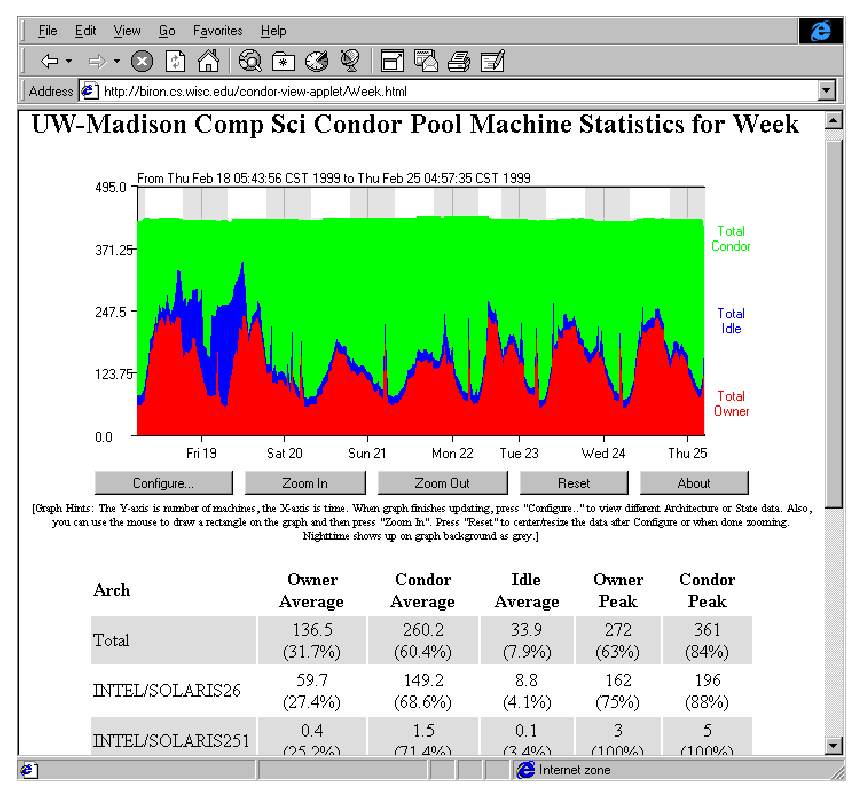
\includegraphics{admin-man/view-screenshot.ps}
\caption{\label{fig:view-screenshot}Screenshot of CondorView Client}
\end{figure}

After unpacking and installing the CondorView Client, a script named
\MakeStats\ can be invoked to create HTML pages displaying Condor usage
for the past hour, day, week, or month.  
By using the Unix \Prog{cron} facility to periodically execute
\MakeStats, Condor pool usage statistics can be kept up to date
automatically.  
This simple model allows the CondorView Client to be installed easily;
no Web server CGI interface is needed.

%%%%%%%%%%%%%%%%%%%%%%%%%%%%%%%%%%%%%%%%%%%%%%%%%%%%%%%%%%%%%%%%%%%%%%
\subsubsection{\label{sec:condorview-client-step-by-step}
Step-by-step installation of the CondorView Client}
%%%%%%%%%%%%%%%%%%%%%%%%%%%%%%%%%%%%%%%%%%%%%%%%%%%%%%%%%%%%%%%%%%%%%%

\begin{enumerate}

\item First, make certain that you have configured your pool's
\Condor{collector} (typically running on the central manager) to log
information to disk in order to provide a persistent, historical
database of pool statistics.  
The CondorView Client makes queries over the network against this
database.  The \Condor{collector} included with version 6.0.x of Condor
does not have this database support; you will need to download and
install the CondorView Server contrib module.  
If you are running Condor
version 6.1 or above, there is no need to install the CondorView Server
contrib module because the \Condor{collector} included in Condor v6.1+
already has the necessary database support.  
To activate the persistent database logging, add the following entries into
the \condor{config} files on your central manager: 
\begin{verbatim}
    POOL_HISTORY_DIR = /full/path/to/directory/to/store/historical/data 
    KEEP_POOL_HISTORY = True 
\end{verbatim}
For full details on these and other \condor{collector} config file
entries, see section~\ref{sec:Collector-Config-File-Entries} on
page~\pageref{sec:Collector-Config-File-Entries}.

\item Create a directory where you would like CondorView to create the
HTML files.  
This directory should be one "published" by a web server, so that HTML
files which exist in this directory can be accessed via a web browser.  
We will refer to this directory as the \emph{VIEWDIR} directory.

\item Unpack/untar the CondorView Client contrib module into the VIEWDIR.
This will create several files and subdirectories in the VIEWDIR.

\item Edit the file \MakeStats.  At the top of this file are six parameters
you need to customize.  The parameters are:

\begin{description}

	\item[\Macro{ORGNAME}] Set to be a very brief name identifying
	your organization, for example ``Univ of Wisconsin''.  Do not
	use any slashes in the name or other special regular-expression
	characters, i.e. avoid characters like: / $\backslash$ \^\ \$.

	\item[\Macro{CONDORADMIN}] Set to the email
	address of the Condor administrator at your site.  
	This email address will appear at the bottom of the web pages.

	\item[\Macro{VIEWDIR}] Set to the full pathname
	(\Bold{not} a relative path) to the VIEWDIR directory you selected
	in installation step \#2 above.  
	It is the same directory where the \MakeStats\ file lives.

	\item[\Macro{STATSDIR}]  Set to the full
	pathname of the \Bold{directory} which contains the \Condor{stats}
	binary.  
	The \Condor{stats} program is included in the \Release{bin}
	directory with Condor version 6.1 and above; for Condor version
	6.0x, the \Condor{stats} program can be found in the CondorView
	Server contrib module.  
	The value for \Macro{STATSDIR} is added to the \Macro{PATH}
	parameter by default; see below.  

	\item[\Macro{PATH}] Set to a list of subdirectories,
	separated by colons, where the \MakeStats\ script can find
	\Prog{awk}, \Prog{bc}, \Prog{sed}, \Prog{date}, and \Condor{stats}
	programs.  
	If you have \Prog{perl} installed on this system, set the path to
	include the directory where \Prog{perl} is installed as well.  Using
	the below default works on most systems:
\begin{verbatim} 
        PATH=/bin:/usr/bin:$STATSDIR:/usr/local/bin
\end{verbatim}

\end{description}

	\item Now type: 
\begin{verbatim}
        ./make_stats setup  
\end{verbatim}
	This will create all of the initial HTML files.  Open up the file
	\File{index.html} and verify things look good.

	\item Add the \MakeStats\ program to cron.  Running ``\MakeStats\ 
	setup'' in step 5 should have created a \File{cronentries} file.
	This \File{cronentries} file is ready to be processed by your Unix
	system's \Prog{crontab} command.  Enter ``man crontab'' on your
	system if you are not familiar with the \Prog{crontab} command
	and/or the \Prog{cron} daemon.  Take a look at the
	\File{cronentries} file; by default, it will run ``\MakeStats\ hour''
	every 15 minutes, ``\MakeStats\ day'' once an hour, ``\MakeStats\ 
	week'' twice per day, and ``\MakeStats\ month'' once per day.  These
	are reasonable defaults.  You can add these commands to cron on any
	system that can access to the \MacroU{VIEWDIR} and
	\MacroU{STATSDIR}, even on a system that does not have Condor
	installed.  The commands do not have to run as user root either; in
	fact, they should probably not run as root.  These commands can run
	as any user that has read/write access to the VIEWDIR.  To add these
	commands to cron, enter : 
\begin{verbatim} 
        crontab cronentries
\end{verbatim}

	\item That's it!  Point your web browser at the VIEWDIR directory,
	and you should be all set.

\end{enumerate}


%%%%%%%%%%%%%%%%%%%%%%%%%%%%%%%%%%%%%%%%%%%%%%%%%%%%%%%%%%%%%%%%%%%%%%
\section{\label{sec:Ckpt-Server} The Checkpoint Server}
%%%%%%%%%%%%%%%%%%%%%%%%%%%%%%%%%%%%%%%%%%%%%%%%%%%%%%%%%%%%%%%%%%%%%%

\index{installation!checkpoint server}
\index{checkpoint server!installation|(}
\index{HTCondor daemon!condor\_ckpt\_server@\Condor{ckpt\_server}}
\index{daemon!condor\_ckpt\_server@\Condor{ckpt\_server}}
\index{condor\_ckpt\_server daemon}
A Checkpoint Server maintains a repository for checkpoint files.
Within HTCondor, checkpoints may be produced only for standard universe jobs.
Using checkpoint servers reduces the disk requirements of submitting
machines in the pool, since the submitting machines no longer need to
store checkpoint files locally.
Checkpoint server machines should have a large amount of disk space
available, and they should have a fast connection to machines
in the HTCondor pool.

If the spool directories are on a network file system, then
checkpoint files will make two trips over the network: one between the
submitting machine and the execution machine, and a second between the
submitting machine and the network file server.
A checkpoint server configured to use the server's local disk
means that the checkpoint file will travel only once over the
network, between the execution machine and the checkpoint server.
The pool may also obtain checkpointing network performance benefits by
using multiple checkpoint servers, as discussed below.

Note that it is a good idea to pick very stable machines for the checkpoint
servers.
If individual checkpoint servers crash, the HTCondor system will continue to
operate, although poorly.  
While the HTCondor system will recover from a checkpoint server crash
as best it can, there are two problems that can and will occur:
\begin{enumerate}

\item A checkpoint cannot be sent to a checkpoint server that
is not functioning.
Jobs will keep trying to contact the checkpoint server, backing
off exponentially in the time they wait between attempts.
Normally, jobs only have a limited time to checkpoint before they are
kicked off the machine.
So, if the checkpoint server is down for a long period of time,
chances are that a lot of work will be lost by jobs being killed 
without writing a checkpoint. 

\item If a checkpoint is not available from the checkpoint server,
a job cannot be retrieved, and it will either have to be restarted from
the beginning, or the job will wait for the server to come back on line.
This behavior is controlled with the
\Macro{MAX\_DISCARDED\_RUN\_TIME} configuration variable.
This variable represents the maximum amount of CPU time the job is
willing to discard, by starting a job over from its beginning if the
checkpoint server is not responding to requests.

\end{enumerate}

%%%%%%%%%%%%%%%%%%%%%%%%%%%%%%%%%%%%%%%%%%%%%%%%%%%%%%%%%%%%%%%%%%%%%%
\subsection{\label{Prepare-Ckpt-Server} Preparing to Install
a Checkpoint Server} 
%%%%%%%%%%%%%%%%%%%%%%%%%%%%%%%%%%%%%%%%%%%%%%%%%%%%%%%%%%%%%%%%%%%%%%

The location of checkpoint files changes upon the installation
of a checkpoint server.
A configuration change will cause 
currently queued jobs with checkpoints
to not be able to find their checkpoints.
This results in the jobs with checkpoints
remaining indefinitely queued,
due to the lack of finding their checkpoints.
It is therefore best to 
either remove jobs from the queues or let them complete
before installing a checkpoint server.
It is advisable to shut the pool down before doing any
maintenance on the checkpoint server.  
See section~\ref{sec:Pool-Management} on
page~\pageref{sec:Pool-Management} for details on shutting
down the pool. 

A graduated installation of the checkpoint server may be
accomplished by 
configuring submit machines as their queues empty.

%%%%%%%%%%%%%%%%%%%%%%%%%%%%%%%%%%%%%%%%%%%%%%%%%%%%%%%%%%%%%%%%%%%%%%
\subsection{\label{Install-Ckpt-Server-Module}
Installing the Checkpoint Server Module} 
%%%%%%%%%%%%%%%%%%%%%%%%%%%%%%%%%%%%%%%%%%%%%%%%%%%%%%%%%%%%%%%%%%%%%%

The files relevant to a checkpoint server are
\begin{verbatim}
        sbin/condor_ckpt_server
        etc/examples/condor_config.local.ckpt.server
\end{verbatim}

\File{\condor{ckpt\_server}} is the checkpoint server binary.
\File{\condor{condor\_config.local.ckpt.server}} is an example
configuration for a checkpoint server. The settings embodied in this
file must be customized with site-specific information.

There are three steps necessary towards running a checkpoint server:
\begin{enumerate}
\item Configure the checkpoint server.
\item Start the checkpoint server.
\item Configure the pool to use the checkpoint server.
\end{enumerate}


\begin{description}

\item[Configure the Checkpoint Server]

\index{checkpoint server!configuration of}
Place settings in the local configuration file of
the checkpoint server.
The file \File{etc/examples/condor\_config.local.ckpt.server} contains
a template for the needed configuration. Insert these into the local
configuration file of the checkpoint server machine. 

The value of \Macro{CKPT\_SERVER\_DIR}  
must be customized.
This variable defines the location of checkpoint files.
It is better if this location is within a very fast local file system,
and preferably a RAID. 
The speed of this file system will have a direct impact on the speed
at which checkpoint files can be retrieved from the remote machines. 

The other optional variables are:
\begin{description}

\item[\Macro{DAEMON\_LIST}] Described in
section~\ref{sec:Master-Config-File-Entries}.  
To have the checkpoint server managed by the \Condor{master},
the \MacroNI{DAEMON\_LIST} variable's value must list both \Expr{MASTER}
and \Expr{CKPT\_SERVER}.
Also add \Expr{STARTD} to allow jobs to run on the checkpoint server machine.
Similarly, add \Expr{SCHEDD} to permit the submission of jobs from the
checkpoint server machine. 

\end{description}

The remainder of these variables are the checkpoint server-specific versions
of the HTCondor logging entries, as described in
section~\ref{sec:Daemon-Logging-Config-File-Entries} on
page~\pageref{sec:Daemon-Logging-Config-File-Entries}.
\begin{description}

\item[\Macro{CKPT\_SERVER\_LOG}] The location of the checkpoint server log.

\item[\Macro{MAX\_CKPT\_SERVER\_LOG}] Sets the maximum
size of the checkpoint server log, before it is saved and the
log file restarted.

\item[\Macro{CKPT\_SERVER\_DEBUG}] Regulates the amount of information
printed in the log file.
Currently, the only debug level supported is \Dflag{ALWAYS}.

\end{description}

\item[Start the Checkpoint Server]

To start the newly configured checkpoint server,
restart HTCondor on that host to enable
the \Condor{master} to notice the new configuration.
Do this by sending a \Condor{restart} command from any machine
with administrator access to the pool.
See section~\ref{sec:Host-Security} on
page~\pageref{sec:Host-Security} for full details about IP/host-based
security in HTCondor. 

Note that when the \Condor{ckpt\_server} starts up, it will immediately
inspect any checkpoint files in the location described by the
\MacroNI{CKPT\_SERVER\_DIR} variable, and determine if any of them are stale.
Stale checkpoint files will be removed.

\item[Configure the Pool to Use the Checkpoint Server]

After the checkpoint server is running,
modify a few configuration variables to let the other machines in the pool
know about the new server:

\begin{description}
   \item[\Macro{USE\_CKPT\_SERVER}] A boolean value that should be set to
   \Expr{True} to enable the use of the checkpoint server.

   \item[\Macro{CKPT\_SERVER\_HOST}] Provides the full host name 
   of the machine that is now running the checkpoint server.  
\end{description}

It is most convenient to set these variables in the pool's
global configuration file,
so that they affect all submission machines.
However, it is permitted to configure each submission machine separately
(using local configuration files), for example if it is desired that not all
submission machines begin using the checkpoint server at one time.
If the variable \MacroNI{USE\_CKPT\_SERVER} is set to \Expr{False},
the submission machine will not use a checkpoint server.

Once these variables are in place,
send the command \Condor{reconfig} to all machines in the pool,
so the changes take effect.
This is described in section~\ref{sec:Reconfigure-Pool} on
page~\pageref{sec:Reconfigure-Pool}.

\end{description}

%%%%%%%%%%%%%%%%%%%%%%%%%%%%%%%%%%%%%%%%%%%%%%%%%%%%%%%%%%%%%%%%%%%%%%
\subsection{\label{Configure-Multiple-Ckpt-Server} 
Configuring the Pool to Use Multiple Checkpoint Servers}
%%%%%%%%%%%%%%%%%%%%%%%%%%%%%%%%%%%%%%%%%%%%%%%%%%%%%%%%%%%%%%%%%%%%%%

\index{checkpoint server!multiple servers}

An HTCondor pool may use multiple checkpoint servers.
The deployment of
checkpoint servers across the
network improves the performance of checkpoint production.
In this case, HTCondor machines are configured to send checkpoints to the
\emph{nearest} checkpoint server.
There are two main performance benefits to deploying multiple checkpoint
servers:
\begin{itemize}
\item Checkpoint-related network traffic is localized by
intelligent placement of checkpoint servers.
\item Better performance implies that jobs spend less time
dealing with checkpoints, and more time doing useful work,
leading to jobs having a higher success rate before returning a
machine to its owner, and workstation
owners see HTCondor jobs leave their machines quicker.
\end{itemize}

With multiple checkpoint servers running in the pool, the
following configuration changes are required to make them active.

Set \Macro{USE\_CKPT\_SERVER} to \Expr{True} (the default) on all
submitting machines where HTCondor jobs should use a checkpoint server.
Additionally, variable \Macro{STARTER\_CHOOSES\_CKPT\_SERVER} should be set to
\Expr{True} (the default) on these submitting machines.
When \Expr{True}, this variable specifies that the checkpoint server
specified by the machine running the job should be used instead of the
checkpoint server specified by the submitting machine.
See section~\ref{sec:Checkpoint-Server-Config-File-Entries} on
page~\pageref{sec:Checkpoint-Server-Config-File-Entries} for more
details.
This allows the job to use the checkpoint server closest to the
machine on which it is running, instead of the server closest to the
submitting machine.
For convenience, set these parameters in the
global configuration file.

Second, set \Macro{CKPT\_SERVER\_HOST} on each machine.
This identifies the full host name of the checkpoint server machine,
and should be the host name of the nearest server to the machine.
In the case of multiple checkpoint servers, set this
in the local configuration file.

Third, send a
\Condor{reconfig} command to all machines in the pool, 
so that the changes take effect.
This is described in section~\ref{sec:Reconfigure-Pool} on
page~\pageref{sec:Reconfigure-Pool}.

After completing these three steps, the jobs in the pool will
send their checkpoints to the nearest checkpoint server.
On restart, a job will remember where its checkpoint was
stored and retrieve it from the appropriate server.
After a job successfully writes a checkpoint to a new server, it will
remove any previous checkpoints left on other servers.

Note that if the configured checkpoint server is unavailable,
the job will keep trying to contact that server.
It will not use alternate checkpoint servers.
This may change in future versions of HTCondor.

%%%%%%%%%%%%%%%%%%%%%%%%%%%%%%%%%%%%%%%%%%%%%%%%%%%%%%%%%%%%%%%%%%%%%%
\subsection{\label{Checkpoint-Server-Domains} 
Checkpoint Server Domains}
%%%%%%%%%%%%%%%%%%%%%%%%%%%%%%%%%%%%%%%%%%%%%%%%%%%%%%%%%%%%%%%%%%%%%%

The configuration described in the previous section ensures that jobs
will always write checkpoints to their nearest checkpoint server.  In
some circumstances, it is also useful to configure HTCondor to localize
checkpoint read transfers, which occur when the job restarts from its
last checkpoint on a new machine.  To localize these transfers, 
it is desired
to schedule the job on a machine which is near the checkpoint
server on which the job's checkpoint is stored.

In terminology, all of the machines configured to use checkpoint
server \Term{A} are in \Term{checkpoint server domain A}.
To localize checkpoint transfers, 
jobs which run on machines in a given
checkpoint server domain should continue running on machines in that domain,
thereby transferring checkpoint files in a single local area of the network.
There are two possible configurations which specify what a
job should do when there are no available machines in its checkpoint
server domain:
\begin{itemize}
\item The job can remain idle until a workstation in its checkpoint
server domain becomes available.
\item The job can try to immediately begin executing on a machine
in another checkpoint server domain.  In this case, the job transfers
to a new checkpoint server domain.
\end{itemize}
These two configurations are described below.

The first step in implementing checkpoint server domains is to include
the name of the nearest checkpoint server in the machine
ClassAd, so this information can be used in job scheduling decisions.
To do this, add the following configuration to each machine:
\begin{verbatim}
  CkptServer = "$(CKPT_SERVER_HOST)"
  STARTD_ATTRS = $(STARTD_ATTRS), CkptServer
\end{verbatim}
For convenience, set these variables in the global configuration file.
Note that this example assumes that
\MacroNI{STARTD\_ATTRS} is previously defined in the configuration.
If not, then use the following configuration instead:
\begin{verbatim}
  CkptServer = "$(CKPT_SERVER_HOST)"
  STARTD_ATTRS = CkptServer
\end{verbatim}
With this configuration, all machine ClassAds will include a \AdAttr{CkptServer}
attribute, which is the name of the checkpoint server closest to this
machine.  So, the \AdAttr{CkptServer} attribute defines the checkpoint
server domain of each machine.

To restrict jobs to one checkpoint server domain,
modify the jobs' \AdAttr{Requirements} expression as follows:
\footnotesize
\begin{verbatim}
  Requirements = ((LastCkptServer == TARGET.CkptServer) || (LastCkptServer =?= UNDEFINED))
\end{verbatim}
\normalsize
This \AdAttr{Requirements} expression uses the \AdAttr{LastCkptServer}
attribute in the job's ClassAd, which specifies where the job last
wrote a checkpoint, and the \AdAttr{CkptServer} attribute in the
machine ClassAd, which specifies the checkpoint server domain.  If the
job has not yet written a checkpoint, the \AdAttr{LastCkptServer}
attribute will be \Expr{Undefined}, and the job will be able to execute in
any checkpoint server domain.  However, once the job performs a
checkpoint,
\AdAttr{LastCkptServer} will be defined and the job will be restricted to the
checkpoint server domain where it started running.

To instead allow jobs to transfer to other checkpoint
server domains when there are no available machines in the current
checkpoint server domain, modify the jobs' \AdAttr{Rank} expression
as follows:
\footnotesize
\begin{verbatim}
  Rank = ((LastCkptServer == TARGET.CkptServer) || (LastCkptServer =?= UNDEFINED))
\end{verbatim}
\normalsize
This \AdAttr{Rank} expression will evaluate to 1 for machines in the
job's checkpoint server domain and 0 for other machines.  So, the job
will prefer to run on machines in its checkpoint server domain, but if
no such machines are available, the job will run in a new checkpoint
server domain.

The checkpoint server domain \AdAttr{Requirements} or \AdAttr{Rank} expressions 
can be automatically appended 
to all standard universe jobs submitted in the pool using
the configuration variables
\MacroNI{APPEND\_REQ\_STANDARD} or \MacroNI{APPEND\_RANK\_STANDARD}.
See section~\ref{sec:Submit-Config-File-Entries} on
page~\pageref{sec:Submit-Config-File-Entries} for more details.
\index{checkpoint server!installation|)}

%%%%%%%%%%%%%%%%%%%%%%%%%%%%%%%%%%%%%%%%%%%%%%%%%%%%%%%%%%%%%%%%%%%%%%
\subsection{Installing PVM Support in Condor}
\label{sec:Install-PVM-Condor}
%%%%%%%%%%%%%%%%%%%%%%%%%%%%%%%%%%%%%%%%%%%%%%%%%%%%%%%%%%%%%%%%%%%%%%

\Todo


%%%%%%%%%%%%%%%%%%%%%%%%%%%%%%%%%%%%%%%%%%%%%%%%%%%%%%%%%%%%%%%%%%%%%%
\subsection{\label{sec:EventD}
Condor Event Daemon}
%%%%%%%%%%%%%%%%%%%%%%%%%%%%%%%%%%%%%%%%%%%%%%%%%%%%%%%%%%%%%%%%%%%%%%

\index{daemon!eventd}
\index{event daemon}
\index{contrib module!event daemon}

The event daemon is an administrative tool for scheduling events in a
Condor pool.
Every \Macro{EVENTD\_INTERVAL}, for each defined event, the event
daemon (eventd) computes an estimate of the time required to complete or
prepare for the event.  If the time required is less than the time
between the next interval and the start of the event, the event daemon
activates the event.

Currently, this daemon supports \Macro{SHUTDOWN} events, which place machines
in the owner state during scheduled times.
The eventd causes machines to vacate jobs one at a time
in anticipation of \Macro{SHUTDOWN} events.
Scheduling this improves performance, because the machines
do not all attempt to checkpoint their jobs at the same time.
To determine the estimate of the time required to complete a \Macro{SHUTDOWN}
event, the \Attr{ImageSize} values for all running standard universe jobs are
totalled and then divided by the maximum bandwidth specified for this
event.

When a \Macro{SHUTDOWN} event is activated, the eventd contacts all startd
daemons
that match constraints given in the configuration file,
and instructs them to shut down.
In response to this instruction,
the startd on any machine not running a job will immediately transition to
the owner state.
Any machine currently running a job will continue to run the
job, but will not start any new job.
The eventd then sends a vacate command to the each startd
that is currently running a job.
Once the job is vacated, the startd transitions to the
owner state.

\Condor{eventd} must run on a machine with administrator
access to your pool.
See section~\ref{sec:Host-Security} on
page~\pageref{sec:Host-Security} for full details about IP/host-based
security in Condor.

%%%%%%%%%%%%%%%%%%%%%%%%%%%%%%%%%%%%%%%%%%%%%%%%%%%%%%%%%%%%%%%%%%%%%%
\subsubsection{\label{sec:EventD-Installation}
Installing the Event Daemon} 
%%%%%%%%%%%%%%%%%%%%%%%%%%%%%%%%%%%%%%%%%%%%%%%%%%%%%%%%%%%%%%%%%%%%%%

\Condor{eventd} requires version 6.1.3 or later of
\Condor{startd}.
So, you should first install either the latest version of the SMP
\Condor{startd} contrib module or the latest release of Condor version
6.1.

First, download the \Condor{eventd} contrib module.
Uncompress and untar the file, to have a directory that
contains a \File{eventd.tar}.
The \File{eventd.tar} acts much like the \File{release.tar} file from
a main release.
This archive contains the files:
\begin{verbatim}
	sbin/condor_eventd
	etc/examples/condor_config.local.eventd
\end{verbatim}
These are all new files, not found in the main release, so you can
safely untar the archive directly into your existing release
directory.
The file \File{\condor{eventd}} is the eventd binary.
The example configuration file is described below.

%%%%%%%%%%%%%%%%%%%%%%%%%%%%%%%%%%%%%%%%%%%%%%%%%%%%%%%%%%%%%%%%%%%%%%
\subsubsection{\label{sec:EventD-Configuration}
Configuring the Event Daemon} 
%%%%%%%%%%%%%%%%%%%%%%%%%%%%%%%%%%%%%%%%%%%%%%%%%%%%%%%%%%%%%%%%%%%%%%

The file \File{etc/examples/condor\_config.local.eventd} contains an
example configuration.
To define events, first set the \Macro{EVENT\_LIST} macro.
This macro contains a list of macro names which define the individual
events.
The definition of individual events depends on the type of the event.
Currently, there is only one event type: \Macro{SHUTDOWN}.
The format for \Macro{SHUTDOWN} events is
\begin{verbatim}
	SHUTDOWN DAY TIME DURATION BANDWIDTH CONSTRAINT RANK
\end{verbatim}
\verb@TIME@ and \verb@DURATION@ are specified in an hours:minutes format.

For example:
\index{event daemon!example configuration}
\begin{verbatim}
EVENT_LIST	= TestEvent, TestEvent2
TestEvent	= SHUTDOWN W 16:00 1:00 2.5 TestEventConstraint TestEventRank
TestEvent2	= SHUTDOWN F 14:00 0:30 6.0 TestEventConstraint2 TestEventRank
TestEventConstraint		= (Arch == "INTEL")
TestEventConstraint2		= (True)
TestEventRank			= (0 - ImageSize)
\end{verbatim}

In this example, the \verb@TestEvent@ is a \Macro{SHUTDOWN} type event, which
specifies that all machines whose startd ads match the constraint
\verb@Arch == "INTEL"@ should be shutdown for one hour starting at
16:00 every Wednesday, and no more than 2.5 Mbytes/s of bandwidth
should be used to vacate jobs in anticipation of the shutdown
event.  According to the \verb@TestEventRank@, jobs will be vacated in
reverse order of their \Attr{ImageSize} (larger jobs first, smaller jobs
last).  \verb@TestEvent2@ is a \Macro{SHUTDOWN} type event, which specifies
that all machines should be shutdown for 30 minutes starting at
14:00 every Friday, and no more than 6.0 Mbytes/s of bandwidth should
be used to vacate jobs in anticipation of the shutdown event.

Note that the \Macro{DAEMON\_LIST} macro (described in
section~\ref{sec:Master-Config-File-Entries}) is defined in the
section of settings you may want to customize.
If you want the event daemon managed by the \Condor{master}, the
\Macro{DAEMON\_LIST} entry must contain both 
\Attr{MASTER} and \Attr{EVENTD}.
Verify that this macro is set to run the correct daemons on
this machine.  By default, the list also includes
\Attr{SCHEDD} and \Attr{STARTD}.

See section~\ref{sec:Eventd-Config-File-Entries} on
page~\pageref{sec:Eventd-Config-File-Entries} for a description of
optional event daemon parameters.

%%%%%%%%%%%%%%%%%%%%%%%%%%%%%%%%%%%%%%%%%%%%%%%%%%%%%%%%%%%%%%%%%%%%%%
\subsubsection{\label{sec:Start-EventD} 
Starting the Event Daemon} 
%%%%%%%%%%%%%%%%%%%%%%%%%%%%%%%%%%%%%%%%%%%%%%%%%%%%%%%%%%%%%%%%%%%%%%

To start an event daemon once it is configured to run on a given
machine, restart Condor on that given machine to enable
the \Condor{master} to notice the new configuration.
Send a \Condor{restart} command from any machine
with administrator access to your pool.
See section~\ref{sec:Host-Security} on
page~\pageref{sec:Host-Security} for full details about IP/host-based
security in Condor.







%%%%%%%%%%%%%%%%%%%%%%%%%%%%%%%%%%%%%%%%%%%%%%%%%%%%%%%%%%%%%%%%%%%%%%
\section{\label{sec:UserPrio}
User Priorities}
%%%%%%%%%%%%%%%%%%%%%%%%%%%%%%%%%%%%%%%%%%%%%%%%%%%%%%%%%%%%%%%%%%%%%%

% Karen's understanding of this stuff, in preparation for a re-write
% of the section:

% Users request machines (by submitting jobs).
% Each user has a calculated priority.
%   A larger priority is worse.
%   This priority essentially tells how many machines the user is
%   currently using.  The priority can be made worse (larger number)
%   by the settings of various configuration variables.
% During each negotiation cycle, all machines are allocated (presuming
%   that there are more requests than machines).
% Each user is allocated machines in a ratio of 1/users's priority.
% Within the negotiation cycle, each user is given an initial
%   allocation of machines.  From there, remaining unallocated machines
%   are divided up among users that want more.  In a round robin
%   manner, each user is allocated a fraction of the remaining
%   unallocated machines.  this fraction is 1/user's priority.

\index{priority!in machine allocation}
\index{user priority}
Condor uses priorities to determine machine allocation for jobs.
This section details the priorities.

For accounting purposes, each user is identified by username@uid\_domain.
Each user is assigned a priority value even if submitting jobs from
different machines in the same domain, or even if submitting from multiple
machines in the different domains.

The numerical priority value assigned to a user is inversely related to the 
\emph{goodness} of the priority.
A user with a numerical priority of 5 gets 
more resources than a user with a numerical priority of 50.
There are two 
priority values assigned to Condor users:
\begin{itemize}
	\item Real User Priority (RUP), which measures resource usage of the 
		user.
	\item Effective User Priority (EUP), which determines the number of
		resources the user can get.
\end{itemize}
This section describes these two priorities and how they affect resource
allocations in Condor.
Documentation on configuring and controlling 
priorities may be found in section~\ref{sec:Negotiator-Config-File-Entries}.

\subsection{Real User Priority (RUP)}
\index{real user priority (RUP)}
\index{user priority!real (RUP)}
A user's RUP measures the resource usage of the user 
through time.
Every user begins with a RUP of one half (0.5), and
at steady state, the RUP of a user equilibrates to the number of resources 
used by that user.  Therefore, if a specific user continuously uses exactly 
ten resources for a long period of time, the RUP of that user stabilizes at 
ten.

However, if the user decreases the number of resources used, the RUP
gets better.  The rate at which the priority value decays 
can be set by the macro \Macro{PRIORITY\_HALFLIFE}, a time period 
defined in seconds.   Intuitively, if the \Macro{PRIORITY\_HALFLIFE} in a pool 
is set to 86400 (one day), and if a user whose RUP was 10 removes all his 
jobs, the user's RUP would be 5 one day later, 2.5 two days later,
and so on.

\subsection{Effective User Priority (EUP)}
\index{effective user priority (EUP)}
\index{user priority!effective (EUP)}
The effective user priority (EUP) of a user is used to determine
how many resources that user may receive.
The EUP is linearly related to the RUP
by a \emph{priority factor} which may be defined on a per-user basis.
Unless otherwise configured, the priority factor for all users is 1.0,
and so the EUP is the same as the the RUP.
However, if desired, the priority factors of
specific users (such as remote submitters) can be increased so that 
others are served preferentially.

The number of resources that a user may receive is inversely related
to the ratio between the EUPs of submitting users.
Therefore user $A$ with EUP=5 will receive
twice as many resources as user $B$ with EUP=10 and four times as many 
resources as user $C$ with EUP=20.
However, if $A$ does not use the full number
of allocated resources,
the available resources are repartitioned and distributed among
remaining users according to the inverse ratio rule.

% editted to here

Condor supplies mechanisms to directly support two policies in which EUP may
be useful:
\begin{description}
	\item[Nice users]  A job may be submitted with the parameter 
	\AdAttr{nice\_user} set to TRUE in the submit command file.
	A nice user job gets its RUP boosted by the 
	\Macro{NICE\_USER\_PRIO\_FACTOR} priority factor specified in the 
	configuration file, leading to a (usually very large) EUP.
	This corresponds to a low priority for resources.
	These jobs are therefore equivalent to Unix background jobs,
	which use resources not used by other Condor users.

	\item[Remote Users] The flocking feature of Condor (see
	section~\ref{sec:Flocking}) allows the \Condor{schedd} to
	submit to more than one pool.
	In addition, the submit-only feature allows a user to run a
	\Condor{schedd} that is submitting jobs into another pool.
	In such situations, submitters from other domains
	can submit to the local pool.
	It is often desirable to have Condor treat local users
	preferentially over these remote users.
	If configured, Condor will boost the RUPs of remote users by
	\Macro{REMOTE\_PRIO\_FACTOR}
	specified in the configuration file,
	thereby lowering their priority for resources.
\end{description}

The priority boost factors for individual users can be set with the 
\Opt{setfactor} option of \Condor{userprio}.
Details may be found in the \Condor{userprio} manual page 
on page~\pageref{man-condor-userprio}.

\subsection{Priorities and Preemption}
\index{preemption!priority}
Priorities are used to ensure that users get their fair share of resources.  
The priority values are used at allocation time.
In addition, Condor preempts machine claims and reallocates them when
conditions change.

To ensure that preemptions do not lead to \Term{thrashing},
a \Macro{PREEMPTION\_REQUIREMENTS} expression is defined to specify the
conditions that must be met for a preemption to occur.
It is usually defined to deny preemption if a current running job
has been running for a relatively short period of time.
This effectively limits the number of preemptions per resource per time
interval.

Note that \MacroNI{PREEMPTION\_REQUIREMENTS} only applies to preemptions
due to user priority.  It does not have any effect if the machine rank
expression prefers a different job, or if the startd policy expression
causes the job to vacate due to other activity on the machine.

\subsection{Priority Calculation}
This section may be skipped if the reader so feels, but for the curious,
here is Condor's priority calculation algorithm.

The RUP of a user $u$ at time $t$, $\pi_r(u,t)$, is calculated 
every time interval $\delta t$ using the formula 
$$\pi_r(u,t) = \beta\times\pi(u,t-\delta t) + (1-\beta)\times\rho(u,t)$$
where $\rho(u,t)$ is the number of resources used by user $u$ at time $t$,
and $\beta=0.5^{{\delta t}/h}$. $h$ is the half life period set by 
\Macro{PRIORITY\_HALFLIFE}.

The EUP of user $u$ at time $t$, $\pi_e(u,t)$
is calculated by
$$\pi_e(u,t) = \pi_r(u,t)\times f(u,t)$$
where $f(u,t)$ is the priority boost factor for user $u$ at time $t$.

As mentioned previously, the RUP calculation is designed so that at steady
state, each user's RUP stabilizes at the number of resources used by that user. 
The definition of $\beta$ ensures that the calculation of $\pi_r(u,t)$ can be 
calculated over non-uniform time intervals $\delta t$ without affecting the 
calculation.  The time interval $\delta t$ varies due to events internal to 
the system, but Condor guarantees that unless the central manager machine is 
down, no matches will be unaccounted for due to this variance.

% Derek's explanation:
%  > Preferably the user priority is determined by the number of
%  > processors jobs of the user currently occupy, i.e., the "history"
%  > should not play a role.
%  
%  this is the responsibility of the condor "accountant", which lives
%  inside the condor_negotiator daemon.  the knob you want to turn is
%  called "PRIORITY_HALFLIFE".  think of your user priority as a
%  radioactive substance. :) consider a priority that exactly matches
%  your current resource usage the "stable state", and a priority
%  "contaminated" with past usage "radioactive."  if it's got a long
%  halflife, it takes a long time for your priority to decay back to
%  "normal".  if the halflife is very short, it'll decay very quickly,
%  and will remain very close to your current usage.  so, just set
%  PRIORITY_HALFLIFE to a small floating point value (like 0.0001), and
%  your user priority should always match your current usage.  if you're
%  not using any resources, your priority will go back to the baseline
%  value instantly.

%%%%%%%%%%%%%%%%%%%%%%%%%%%%%%%%%%%%%%%%%%%%%%%%%%%%%%%%%%%%%%%%%%%%%%
\section{\label{sec:Configuring-Policy}
Configuring The Startd Policy}
%%%%%%%%%%%%%%%%%%%%%%%%%%%%%%%%%%%%%%%%%%%%%%%%%%%%%%%%%%%%%%%%%%%%%%

This section describes how to configure the \Condor{startd} to
implement the policy you choose for when remote jobs should start, be
suspended, (possibly) resumed, vacated (with a checkpoint) or killed
(no checkpoint).  This policy is the heart of Condor's balancing act
between the needs and wishes of resource owners (machine owners) and
resource users (people submitting their jobs to Condor).  Please read
this section carefully if you plan to change any of the settings
described below, as getting it wrong can have a severe impact on
either the owners of machines in your pool (in which case they might
ask to be removed from the pool entirely) or the users of your pool
(in which case they might stop using Condor).

Much of this section refers to ClassAd expressions.  You probably want
to read through section~\ref{classad-reference} on ClassAd expressions
before continuing with this.

\Note If you are defining the policy for an SMP (multi-CPU) machine,
be sure to also read section~\ref{sec:Configuring-SMP} on
``Configuring The Startd for SMP Machines''.  
Each \Term{virtual machine} represented by the \condor{startd} on an
SMP machine will have its own \Term{state} and \Term{activity}
(described below). 
In the future, each virtual machine will even be able to have its
own policy defined.
For the rest of this section, whenever you see the word ``machine'',
that really just means an individual virtual machine, if you're
talking about an SMP machine that is showing up as multiple virtual
machines in your pool.  

To define your policy, you basically set a number of expressions in
the config file (see section~\ref{sec:Configuring-Condor} on
``Configuring Condor'' for an introduction to Condor's config files).
These expressions are evaluated in the context of the machine's ClassAd
and the ClassAd of a potential resource request (a job that has been
submitted to Condor).
The expressions can therefore reference attributes from either
ClassAd. 
First, we'll list all the attributes that are included in the Machine's
ClassAd.
Then, we'll list all the attributes that are included in a job
ClassAd. 
Next, we'll explain the the \Expr{START} expression, which describes
to Condor what conditions must be met for the machine to start a job.
Then, we'll describe the \Expr{RANK} expression, which allows you to
specify which kinds of jobs a given machine prefers to run.
Then, we'll discuss in some detail how the \Condor{startd} works, in
particular, the machine \Term{states} and \Term{activities}, to give
you an idea of what is possible for your policy decisions.
Finally, we offer two example policy settings.

%%%%%%%%%%%%%%%%%%%%%%%%%%%%%%%%%%%%%%%%%%%%%%%%%%%%%%%%%%%%%%%%%%%%%%
\subsection{\label{sec:Startd-Attributes}
Startd ClassAd Attributes}
%%%%%%%%%%%%%%%%%%%%%%%%%%%%%%%%%%%%%%%%%%%%%%%%%%%%%%%%%%%%%%%%%%%%%%

The \Condor{startd} represents the machine on which it is running to
the Condor pool.  It publishes a number of characteristics about the
machine in its ClassAd to help in match-making with resource requests.
The values of all these attributes can be found by using
\Prog{\condor{status} -l hostname}.
On an SMP machine, the startd will break the machine up and advertise
it as seperate virtual machines, each with its own name and ClassAd.
The attributes themselves and what they represent are described below:

\begin{description}
%
\item[Activity] : String which describes Condor job activity on the machine.
Can have one of the following values:
	\begin{description}
	\item[``Idle''] : There is no job activity
	\item[``Busy''] : A job is busy running
	\item[``Suspended''] : A job is currently suspended
	\item[``Vacating''] : A job is currently checkpointing
	\item[``Killing''] : A job is currently being killed
	\item[``Benchmarking''] : The startd is running benchmarks
	\end{description}
%
\item[AFSCell] : If the machine is running AFS, this is a string
containing the AFS cell name.
%
\item[Arch] : String with the architecture of the machine.  Typically
one of the following: 
	\begin{description}
	\item[``INTEL''] : Intel CPU (Pentium, Pentium II, etc).
	\item[``ALPHA''] : Digital Alpha CPU
	\item[``SGI''] : Silicon Graphics MIPS CPU
	\item[``SUN4u''] : Sun UltraSparc CPU
	\item[``SUN4x''] : A Sun Sparc CPU other than an UltraSparc, i.e.
sun4m or sun4c CPU found in older Sparc workstations such as the Sparc~10, 
Sparc~20, IPC, IPX, etc.
	\item[``HPPA1''] :  Hewlett Packard PA-RISC 1.x CPU (i.e. PA-RISC    
                      7000 series CPU) based workstation
	\item[``HPPA2''] :  Hewlett Packard PA-RISC 2.x CPU (i.e. PA-RISC    
                      8000 series CPU) based workstation
	\end{description}
%
\item[ClockDay] : The day of the week, where 0 = Sunday, 1 = Monday, \Dots, 6 = Saturday. 
%
\item[ClockMin] : The number of minutes passed since midnight.
%
\item[CondorLoadAvg] : The load average generated by Condor (either
from remote jobs or running benchmarks).
%
\item[ConsoleIdle] : The number of seconds since activity on the system
console keyboard or console mouse has last been detected.
%
\item[Cpus] : Number of CPUs in this machine, i.e. 1 = single CPU machine, 2 = dual
CPUs, etc.
%
\item[CurrentRank] : A float which represents this machine owner's affinity
for running the Condor job which it is currently hosting.  If not
currently hosting a Condor job, CurrentRank is -1.0.
%
\item[Disk] : The amount of disk space on this machine available for
the job in kbytes ( e.g. 23000 = 23 megabytes ).  Specifically, this
is the amount of disk space available in the directory specified in
the Condor configuration files by the \Macro{EXECUTE} macro, minus any
space reserved with the \Macro{RESERVED\_DISK} macro.
%
\item[EnteredCurrentActivity] : Time at which the machine entered the 
current Activity (see \AdAttr{Activity} entry above).  Measured in the
number of seconds since the epoch (00:00:00 UTC, Jan 1, 1970).
%
\item[FileSystemDomain] : a domain name configured by the Condor 
administrator which describes a cluster of machines which all access 
the same networked filesystems usually via NFS or AFS.  
%
\item[KeyboardIdle] : The number of seconds since activity on any
keyboard or mouse associated with this machine has last been detected.
Unlike \AdAttr{ConsoleIdle}, \AdAttr{KeyboardIdle} also takes activity 
on pseudo-terminals into
account (i.e. virtual ``keyboard'' activity from telnet and rlogin
sessions as well).  Note that \AdAttr{KeyboardIdle} will always be equal to or
less than \AdAttr{ConsoleIdle}.
%
\item[KFlops] : Relative floating point performance as determined via a
linpack benchmark.
%
\item[LastHeardForm] : Time when the Condor Central Manager last
received a status update from this machine.  
Expressed as seconds since the epoch (integer value).
Note: This attribute is only inserted by the Central Manager once it
receives the ClassAd.
It is not present in the startd's copy of the ClassAd.
Therefore, you couldn't use this attribute in defining startd
expressions (which you wouldn't want to, anyway).
%
\item[LoadAvg] : A floating point number with the machine's current load
average.
%
\item[Machine] : A string with the machine's fully qualified hostname.
%
\item[Memory] : The amount of RAM in megabytes.
%
\item[Mips] : Relative integer performance as determined via a dhrystone
benchmark.
%
\item[MyType] : The ClassAd type; always set to the literal string ``Machine''.
%
\item[Name] : The name of this resource; typically the same value as
the \AdAttr{Machine} attribute, but could be customized by the site
administrator.
On SMP machines, the startd will divide the CPUs up into seperate
virtual machines, each with with a unique name.
These names will be of the form ``vm\#@full.hostname'', for example,
``vm1@vulture.cs.wisc.edu'', which signifies virtual machine 1 from
vulture.cs.wisc.edu. 
%
\item[OpSys] : String describing the operating system running on this
machine.  For Condor \VersionNotice\ typically one of the following:
	\begin{description}
	\item ``HPUX10'' (for HPUX 10.20)
	\item ``IRIX6''  (for IRIX 6.2, 6.3, or 6.4)
	\item ``LINUX''  (for LINUX 2.0.x kernel systems)
	\item ``LINUX-GLIBC''  (for LINUX systems, using GNU's libc)
	\item ``OSF1''	 (for Digital Unix 4.x)
	\item ``SOLARIS251''
	\item ``SOLARIS26''
	\end{description}
%
\item[Requirements] : A boolean which, when evaluated within the context
of the Machine ClassAd and a Job ClassAd, must evaluate to
TRUE before Condor will allow the job to use this machine.
%
\item[StartdIpAddr] : String with the IP and port address of the
\Condor{startd} daemon which is publishing this Machine ClassAd.
%
\item[State] : String which publishes the machine's Condor state, which
can be:
	\begin{description}
	\item[``Owner''] : The machine owner is using the machine, and
it is unavailable to Condor.
	\item[``Unclaimed''] : The machine is available to run Condor jobs,
but a good match (i.e. job to run here) is either not available or not 
yet found.
	\item[``Matched''] : The Condor Central Manager has found a good
match for this resource, but a Condor scheduler has not yet claimed it.
	\item[``Claimed''] : The machine is claimed by a remote
\Condor{schedd} and is probably running a job.
	\item[``Preempting''] : A Condor job is being preempted (possibly
via checkpointing) in order to clear the machine for either a higher
priority job or because the machine owner wants the machine back.
	\end{description}   % of State
%
\item[TargetType] : Describes what type of ClassAd to match with.
Always set to the string literal ``Job'', because Machine ClassAds
always want to be matched with Jobs, and vice-versa.
%
\item[UidDomain] : a domain name configured by the Condor 
administrator which describes a cluster of machines which all have 
the same "passwd" file entries, and therefore all have the same logins.
%
\item[VirtualMemory] : The amount of currently available virtual memory 
(swap space) expressed in kbytes.

\end{description}


%%%%%%%%%%%%%%%%%%%%%%%%%%%%%%%%%%%%%%%%%%%%%%%%%%%%%%%%%%%%%%%%%%%%%%
\subsection{\label{sec:Job-Attributes}
Job ClassAd Attributes}
%%%%%%%%%%%%%%%%%%%%%%%%%%%%%%%%%%%%%%%%%%%%%%%%%%%%%%%%%%%%%%%%%%%%%%

\Todo

%%%%%%%%%%%%%%%%%%%%%%%%%%%%%%%%%%%%%%%%%%%%%%%%%%%%%%%%%%%%%%%%%%%%%%
\subsection{\label{sec:Start-Expr}
The START expression}
%%%%%%%%%%%%%%%%%%%%%%%%%%%%%%%%%%%%%%%%%%%%%%%%%%%%%%%%%%%%%%%%%%%%%%

The most important expression in the startd (and possibly in all of
Condor) is the \Expr{START} expression.  
This expression describes what conditions must be met for a given
machine to service a resource request (in other words, start someone's
job). 
This expression (like any other expression) can reference attributes
in the machine's ClassAd (such as \Attr{KeyboardIdle}, \Attr{LoadAvg},
etc), or attributes in a potential requester's ClassAd (such as
\Attr{Owner}, \Attr{Imagesize}, even \Attr{Cmd}, the name of the
executable the requester wants to run).
What the \Expr{START} expression evaluates to plays a crucial role in
determining what state and activity the machine is in.

It is technically the \Expr{Requirements} expression that is used for
matching with other jobs.  The startd just always defines the
\Expr{Requirements} expression as the \Expr{START} expression.
However, in situations where the machine wants to make itself
unavailable for further matches, it sets its \Expr{Requirements}
expression to False, not its \Expr{START} expression.  
When the \Expr{START} expression \Term{locally evaluates} to true, the
machine advertises the \Expr{Requirements} expression as ``True'' and
doesn't even publish the \Expr{START} expression.

Normally, the expressions in the machine ClassAd are evaluated against
certain request ClassAds in the \Condor{negotiator} to see if there is
a match, or against whatever request ClassAd currently has claimed the
machine.  However, by locally evaluating an expression, the machine only
evaluates the expression against its own ClassAd.  If an expression
cannot be locally evaluated (because it references other expressions
that are only found in a request ad, such as \Attr{Owner} or
\Attr{Imagesize}), the expression is (usually) undefined.  See the
ClassAd appendix, section~\ref{classad-reference}, for specifics of
how undefined terms are handled in ClassAd expression evaluation. 

\Note If you have machines with lots of real memory and swap space so
  the only scarce resource is CPU time, you could use the
  \Macro{JOB\_RENICE\_INCREMENT} (see
  section~\ref{sec:Starter-Config-File-Entries} on ``\condor{starter}
  Config File Entries'' for details) so that Condor starts jobs on
  your machine with low priority.  Then, you could set
  up your machines with:
\begin{verbatim}
        START : True
        SUSPEND : False
        PREEMPT : False
        KILL : False
\end{verbatim}
  This way, Condor jobs would always run and would never be kicked
  off. 
  However, because they would run with ``nice priority'', interactive 
  response on your machines would not suffer.
  You probably wouldn't even notice Condor was running the jobs, 
  assuming you had enough free memory for the Condor jobs so that you 
  weren't swapping all the time.

%%%%%%%%%%%%%%%%%%%%%%%%%%%%%%%%%%%%%%%%%%%%%%%%%%%%%%%%%%%%%%%%%%%%%%
\subsection{\label{sec:Rank-Expression}
The RANK expression}
%%%%%%%%%%%%%%%%%%%%%%%%%%%%%%%%%%%%%%%%%%%%%%%%%%%%%%%%%%%%%%%%%%%%%%

A machine can be configured to prefer running certain jobs over other
jobs.  This is done via the \Expr{RANK} expression.  This is an
expression, just like any other in the machine's ClassAd.  It can
reference any attribute found in either the machine ClassAd or a
request ad (normally, in fact, it references things in the request
ad).  Probably the most common use of this expression is to configure a
machine to prefer to run jobs from the owner of that machine, or by
extension, a group of machines to prefer jobs from the owners of those
machines.  

For example, imagine you have a small research group with 4 machines:
``tenorsax'', ``piano'', ``bass'' and ``drums''.  These machines are
owned by 4 users: ``coltrane'', ``tyner'', ``garrison'' and ``jones'',
respectively.  

Say there's a large Condor pool in your department, but you spent a
lot of money on really fast machines for your group.  You want to make
sure that if anyone in your group has Condor jobs, they have priority
on your machines.  To achieve this, all you have to do is set the Rank
expression on your machines to refer to the \Attr{Owner} attribute and
prefer requests where that attribute matches one of the people in your
group:
\begin{verbatim}
        RANK : Owner == "coltrane" || Owner == "tyner" \
               || Owner == "garrison" || Owner == "jones"
\end{verbatim}

The \Expr{RANK} expression is evaluated as a floating point number.
However, just like in C, boolean expressions evaluate to either 1 or 0
depending on if they're true or false.  So, if this expression
evaluated to 1 (because the remote job was owned by one of the blessed
folks), that would be higher than anyone else (for whom the expression
would evaluate to 0).

If you wanted to get really fancy, you could still have the same basic
setup, where anyone from your group has priority on your machines, but
the actual machine owner has even more priority on their own machine.
For example, you'd put the following entry in Jimmy Garrison's local
config file \File{bass.local}:
\begin{verbatim}
        RANK : Owner == "coltrane" + Owner == "tyner" \
               + (Owner == "garrison") * 10 + Owner == "jones"
\end{verbatim}
Notice, we're using ``+'' instead of ``\Bar\Bar'', since we want to be able
to distinguish which terms matched and which ones didn't.  Now, if
anyone who wasn't in the John Coltrane quartet was running a job on
``bass'', the \Expr{RANK} would evaluate numerically to 0, since none
of those boolean terms would evaluate to 1, and 0+0+0+0 is still 0.
Now, suppose Elvin Jones submits a job.  His job would match this
machine (assuming the \Expr{START} was true for him at that time) and
the \Expr{RANK} would numerically evaluate to 1 (since one of the
boolean terms would evaluate to 1), so Elvin would preempt whoever
else was using the machine at the time.  After a while, say Jimmy
decides to submit a job (maybe even from another machine, it doesn't
matter, all that matters is that it's Jimmy's job).  Now, the
\Expr{RANK} would evaluate to 10, since the boolean that matches him
gets multiplied by 10.  So, Jimmy would preempt even Elvin, and his
job would run on his machine.

The \Expr{RANK} expression doesn't just have to refer to the
\Attr{Owner} of the jobs.  Suppose you have a machine with a ton of
memory, and others with not much at all.  You could configure your
big-memory machine to prefer to run jobs with bigger memory
requirements:
\begin{verbatim}
        RANK : ImageSize
\end{verbatim}

That's all there is to it.  The bigger the job, the more this machine
wants to run it.  That's pretty altruistic of you, always servicing
bigger and bigger jobs, even if they're not yours.  So, perhaps you
still want to be a nice guy, all else being equal, but if you have
jobs, you want to run them, regardless of everyone else's
\Attr{Imagesize}:
\begin{verbatim}
        RANK : (Owner == "coltrane" * 1000000000000) + Imagesize
\end{verbatim}
This scheme would break down if someone submitted a job with an image
size of more 10\Circum12 kbytes.  However, if they did, this Rank expression
preferring their job over yours wouldn't be the only problem Condor
had. :-)


%%%%%%%%%%%%%%%%%%%%%%%%%%%%%%%%%%%%%%%%%%%%%%%%%%%%%%%%%%%%%%%%%%%%%%
\subsection{\label{sec:States}
Machine States}
%%%%%%%%%%%%%%%%%%%%%%%%%%%%%%%%%%%%%%%%%%%%%%%%%%%%%%%%%%%%%%%%%%%%%%

A given machine could be in a number of different \Term{states},
depending on whether or not the machine is available to run Condor
jobs, and if so, what stage in the Condor protocol has been reached.
The possible states are:

\begin{description}
  
\item[Owner] The machine is being used by the machine owner, or at
  least is not available to run Condor jobs.  When the machine first
  starts up, it begins in this state.
  
\item[Unclaimed] The machine is available to run Condor jobs, but is
  not currently doing so in any way.
  
\item[Matched] The machine is available to run jobs, and has been
  matched by the negotiator with a given schedd.  That schedd just
  hasn't claimed this machine yet.  In this state, the machine is
  unavailable for further matches.

\item[Claimed] The machine has been claimed by a schedd. 
  
\item[Preempting] The machine was claimed by a schedd, but is now
  preempting that claim because either the owner of the machine came
  back, the negotiator decided to preempt this match because another
  user with higher priority has jobs waiting to run, or the negotiator
  decided to preempt this match because it found another request that
  this resource would rather serve (see the \Expr{RANK} expression
  below).

\end{description}

See figure~\ref{fig:machine-states} on page~\pageref{fig:machine-states}
for the various states and the possible transitions between them.

\begin{figure}[hbt]
\centering
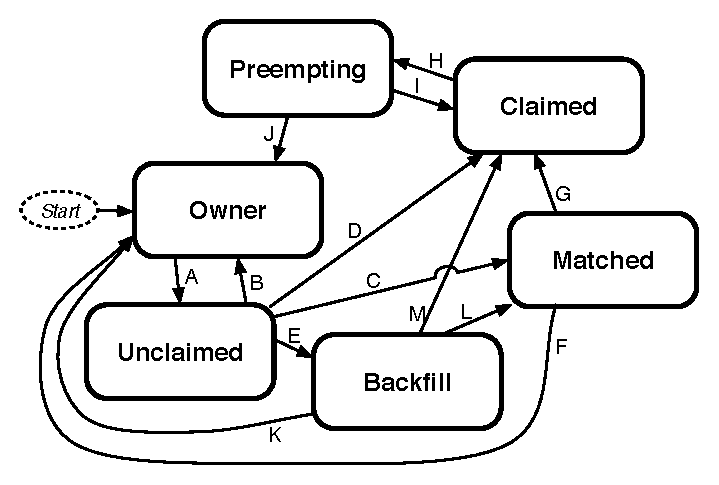
\includegraphics{admin-man/machine-states.eps}
\caption{\label{fig:machine-states}Machine States}
\end{figure}

%%%%%%%%%%%%%%%%%%%%%%%%%%%%%%%%%%%%%%%%%%%%%%%%%%%%%%%%%%%%%%%%%%%%%%
\subsection{\label{sec:Activities}
Machine Activities}
%%%%%%%%%%%%%%%%%%%%%%%%%%%%%%%%%%%%%%%%%%%%%%%%%%%%%%%%%%%%%%%%%%%%%%

Within some of these states, there could be a number of different
\Term{activities} the machine is in.  The idea is that all the things
that are true about a given state are true regardless of what activity
you are in.  However, there are certain important differences between
each activity, which is why they are separated out from each other
within a given state.  In general, you must specify both a state and
an activity to describe what ``state'' the machine is in.  This will be
denoted in this manual as ``state/activity'' pairs.  For example,
``Claimed/Busy''.  The following list describes all the possible
state/activity pairs:

\begin{itemize}

\item Owner
\begin{description}
\item[Idle] This is the only activity for Owner state.  As far as
  Condor is concerned the machine is ``Idle'' (not doing anything for
  Condor).
\end{description}

\item Unclaimed
\begin{description}
  
\item[Idle] This is the normal activity of Unclaimed machines.  The
  machine is still ``Idle'' in that the machine owner is willing to
  let someone run jobs on it, but Condor is still not using the
  machine for anything.
  
\item[Benchmarking] The machine could also be running benchmarks to
  determine the speed on this machine.  It only does this when the
  machine is in the Unclaimed state.  How often it does so is
  determined by the \Expr{RunBenchmarks} expression described below.

\end{description}

\item Matched
\begin{description}
\item[Idle] When Matched, the machine is still ``Idle'' as far as
  Condor is concerned.
\end{description}

\item Claimed
\begin{description}
  
\item[Idle] In this activity, the machine has been claimed, but the
  schedd that claimed it has yet to \Term{activate} the claim by
  requesting a \Condor{starter} to be spawned which would service a
  given job.
  
\item[Busy] Once a \Condor{starter} has been started and the claim is
  active, the machine moves to the Busy activity to signify that it's
  actually doing something as far as Condor is concerned.
  
\item[Suspended] If the job is suspended by Condor, the machine goes
  into the Suspended activity.
  The match between the schedd and machine has not been broken (the
  claim is still valid), but the job is not making any progress and
  Condor is no longer generating a load on the machine.

\end{description}

\item Preempting

  The preempting state is used for evicting a Condor job from a given
  machine.  When the machine enters the Preempting state, it checks the
  \Expr{WANT\_VACATE} expression (described below) to decide which of
  the following activities it should enter:

\begin{description}
  
\item[Vacating] Vacating simply means that the job that was running is
  in the process of checkpointing.  As soon as the checkpoint process
  completes, the machine moves into either the Owner state or the
  Claimed state, depending on why it began preempting in the first
  place.
  
\item[Killing] Killing means that the machine has requested the running
  job to exit the machine immediately, without checkpointing.

\end{description}

\end{itemize}

Figure~\ref{fig:machine-activities} on
page~\pageref{fig:machine-activities} gives the overall view of all
machine states and activities, and shows all the possible transitions
from one to another within the Condor system.  
Each transition is labeled with a number on the diagram, and
transition numbers refered to in this manual will be \Bold{bold}.  
This may seem pretty daunting, but it's actually easier to handle than
it looks.

\begin{figure}[hbt]
\centering
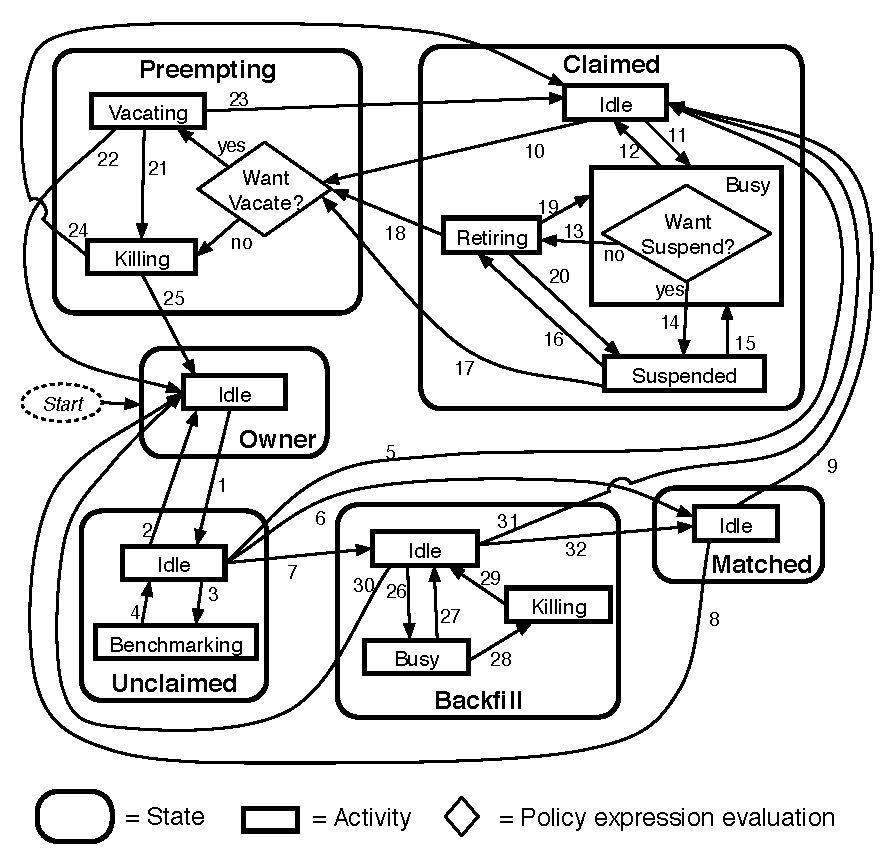
\includegraphics{admin-man/machine-activities.eps}
\caption{\label{fig:machine-activities}Machine States and Activities}
\end{figure}

Various expressions are used to determine when and if many of these
state and activity transitions occur.  Other transitions are initiated
by parts of the Condor protocol (such as when the \Condor{negotiator}
matches a machine with a schedd).  The following section describes the
conditions that lead to the various state and activity transitions.

%%%%%%%%%%%%%%%%%%%%%%%%%%%%%%%%%%%%%%%%%%%%%%%%%%%%%%%%%%%%%%%%%%%%%%
\subsection{\label{sec:State-and-Activity-Transitions}
State and Activity Transitions}
%%%%%%%%%%%%%%%%%%%%%%%%%%%%%%%%%%%%%%%%%%%%%%%%%%%%%%%%%%%%%%%%%%%%%%

This section will trace through all possible state and activity
transitions within the machine and describe the conditions under which
each one occurs.
Whenever a transition occurs, the machine records when it entered its
new activity and/or new state.
These times are often used to write the expressions that determine
when further transitions occurred (for example, you might only enter
the Killing activity if you've been in the Vacating activity longer
than a given amount of time). 

%%%%%%%%%%%%%%%%%%%%%%%%%%%%%%%%%%%%%%%%%%%%%%%%%%%%%%%%%%%%%%%%%%%%%%
\subsubsection{\label{sec:Owner-State}
Owner State}
%%%%%%%%%%%%%%%%%%%%%%%%%%%%%%%%%%%%%%%%%%%%%%%%%%%%%%%%%%%%%%%%%%%%%%

When the startd is first spawned, the machine it represents enters the
Owner state. 
The machine will remain in this state as long as the \Expr{START}
expression locally evaluates to false.
If the \Expr{START} locally evaluates to true or can't be locally
evaluated (it evaluates to \Term{undefined}), transition \Bold{1} will
occur and the machine will enter the Unclaimed state.

So long as the \Expr{START} expression locally evaluates to false,
there is no possible request in the Condor system that could match it,
so the machine in unavailable to Condor and stays in the Owner state.
For example, if the \Expr{START} expression was:
\begin{verbatim}
START : KeyboardIdle > 15 * $(MINUTE) && Owner == "coltrane" 
\end{verbatim}
and if \Attr{KeyboardIdle} was only 34 seconds, then the machine would
still be in the Owner state, even though it references Owner, which is
undefined.  \verb@False && anything@ is False, even 
\verb@False && undefined@

If, however, the \Expr{START} expression was:
\begin{verbatim}
        START : KeyboardIdle > 15 * $(MINUTE) || Owner == "coltrane"
\end{verbatim}
and \Attr{KeyboardIdle} was still only 34 seconds, then the machine
would leave the Owner state and go to Unclaimed.  This is because
``False || undefined'' is undefined.  So, while this machine isn't
available to just any body, if user ``coltrane'' has jobs submitted,
the machine is willing to run them.  Anyone else would have to wait
until \Attr{KeyboardIdle} exceeds 15 minutes.  However, since
``coltrane'' might claim this resource, but hasn't yet, the machine
goes to the Unclaimed state.

While in the Owner state the startd only polls the status of the
machine every \Macro{UPDATE\_INTERVAL} to see if anything has changed
that would lead it to a different state.  The idea is that you don't
want to put much load on the machine while the Owner is using it
(frequently waking up, computing load averages, checking the access
times on files, computing free swap space, etc), and there's nothing
time critical that the startd needs to be sure to notice as soon as it
happens.  If the \Expr{START} expression evaluates to True and it's 5
minutes before we notice it, that's a drop in the bucket of High
Throughput Computing.

The machine can only go to the Unclaimed state from the Owner state,
and only does so when the \Expr{START} expression no longer locally
evaluates to False.  Generally speaking, if the \Expr{START}
expression locally evaluates to false at any time, the machine will
either transition directly to the Owner state, or to the Preempting
state on its way to the Owner state, if there's a job running that
needs preempting.

%%%%%%%%%%%%%%%%%%%%%%%%%%%%%%%%%%%%%%%%%%%%%%%%%%%%%%%%%%%%%%%%%%%%%%
\subsubsection{\label{sec:Unclaimed-State}Unclaimed State}
%%%%%%%%%%%%%%%%%%%%%%%%%%%%%%%%%%%%%%%%%%%%%%%%%%%%%%%%%%%%%%%%%%%%%%

While in the Unclaimed state, if the \Expr{START} expression locally
evalutes to false, the machine will return to the Owner state via
transition \Bold{2}.

When it's in the Unclaimed state, another expression comes into
effect, \Expr{RunBenchmarks} \label{param:RunBenchmarks}.  
Whenever the \Expr{RunBenchmarks} evaluates to True while the machine
is in the Unclaimed state, the machine will transition from the Idle
activity to the Benchmarking activity (transition \Bold{3}) and
perform benchmarks to determine \Attr{MIPS} and \Attr{KFLOPS}.  
When the benchmarks complete, the machine returns to the Idle activity
(transition \Bold{4}).

The startd automatically inserts an attribute, \Attr{LastBenchmark},
whenever it runs benchmarks, so commonly \Attr{LastBenchmark} is
defined in terms of this attribute, for example:
\begin{verbatim}
        BenchmarkTimer = (CurrentTime - LastBenchmark)
        RunBenchmarks : $(BenchmarkTimer) >= (4 * $(HOUR))
\end{verbatim}
Here, a macro, \Macro{BenchmarkTimer} is defined to help write the
expression.  The idea is that this macro holds the time since the last
benchmark, so when this time exceeds 4 hours, we run the benchmarks
again.  The startd keeps a weighted average of these benchmarking
results to try to get the most accurate numbers possible.  That's why
you would want the startd to run them more than once in its lifetime.

\Note LastBenchmark is initialized to 0 before the benchmarks
have ever been run.
So, if you want the startd to run benchmarks as soon as the machine is
unclaimed (if it hasn't done so already), just include a term for
\Attr{LastBenchmark} as in the example above.

\Note If \Expr{RunBenchmarks} is defined, and set to something
other than ``False'', the startd will automatically run one set of
benchmarks when it first starts up.
So, if you want to totally disable benchmarks, both at startup, and at
any time thereafter, just set \Expr{RunBenchmarks} to ``False'' or
comment it out from your config file.

From the Unclaimed state, the machine can go to two other possible
states: Matched or Claimed/Idle.
Once the \Condor{negotiator} matches an Unclaimed machine with a
requester at a given schedd, the negotiator sends a command to both
parties, notifying them of the match.  
If the schedd gets that notification and initiates the claiming
procedure with the machine before the negotiator's message gets to the
machine, the Match state is skipped entirely, and the machine goes
directly to the Claimed/Idle state (transition \Bold{5}).
However, normally the machine will enter the Matched state (transition
\Bold{6}), even if it's only for a brief period of time.

%%%%%%%%%%%%%%%%%%%%%%%%%%%%%%%%%%%%%%%%%%%%%%%%%%%%%%%%%%%%%%%%%%%%%%
\subsubsection{\label{sec:Matched-State}Matched State}
%%%%%%%%%%%%%%%%%%%%%%%%%%%%%%%%%%%%%%%%%%%%%%%%%%%%%%%%%%%%%%%%%%%%%%

The Matched state is not very interesting to Condor.  The only
noteworthy things are that the machine lies about its \Expr{START}
expression while in this state and says that \Expr{Requirements} are
false to prevent being matched again before it has been claimed, and
that the startd starts a timer to make sure it doesn't stay in the
Matched state too long.  This timer is set with the
\Macro{MATCH\_TIMEOUT} \label{param:MatchTimeout} config file
parameter.  It is specified in seconds and defaults to 300 (5
minutes).  If the schedd that was matched with this machine doesn't
claim it within this period of time, the machine gives up on it, goes
back into the Owner state via transition \Bold{7} (which it will
probably leave right away to get to the Unclaimed state again, and
wait for another match). 

At any time while the machine is in the Matched state, if the
\Expr{START} expression locally evaluates to false, the machine enters
the Owner state directly (transition \Bold{7}).

If the schedd that was matched with the machine claims it before the
\Macro{MATCH\_TIMEOUT} expires, the machine goes into the Claimed/Idle
state (transition \Bold{8}).

%%%%%%%%%%%%%%%%%%%%%%%%%%%%%%%%%%%%%%%%%%%%%%%%%%%%%%%%%%%%%%%%%%%%%%
\subsubsection{Claimed State}
\label{sec:Claimed-State}
%%%%%%%%%%%%%%%%%%%%%%%%%%%%%%%%%%%%%%%%%%%%%%%%%%%%%%%%%%%%%%%%%%%%%%

The Claimed state is certainly the most complicated state.
It has the most possible activities, and the most expressions that
determine what it will do next.
In addition the \Condor{checkpoint} and \Condor{vacate} commands only
have any effect on the machine when its in the Claimed state.
In general, there are two sets of expressions that might take effect,
depending on if the universe of the request that claimed the machine is
Standard or Vanilla.
The Standard Universe expressions are the ``normal'' expressions, for
example:
\begin{verbatim}
        WANT_SUSPEND            : True
        WANT_VACATE             : $(ActivationTimer) > 10 * $(MINUTE)
        SUSPEND                 : $(KeyboardBusy) || $(CPUBusy)
        ...
\end{verbatim}

The Vanilla expressions have ``\_VANILLA'' appended to the end, for
example:
\begin{verbatim}
        WANT_SUSPEND_VANILLA    : True
        WANT_VACATE_VANILLA     : True
        SUSPEND_VANILLA         : $(KeyboardBusy) || $(CPUBusy)
        ...
\end{verbatim}

If you don't specify seperate vanilla versions, the normal versions
will be used for all jobs, including vanilla jobs.  
For the purposes of this manual, we'll always refer to the regular 
expressions.
Keep in mind that if the request was a Vanilla Universe, the Vanilla
expressions (if they were defined) would be in effect, instead.
The reason for this is that the resource owner might want the machine
to behave differently for Vanilla jobs, since they can't checkpoint.
For example, they might want to let Vanilla jobs remain suspended for
much longer than standard jobs.

While Claimed, the \Macro{POLLING\_INTERVAL} takes effect, and the
startd starts polling the machine much more frequently to evaluate its
state.

If the owner starts typing on the console again, we want to notice as
soon as possible and start doing whatever that owner wants at that
point.
For SMP machines, if any virtual machine is in the Claimed state, the
startd will poll the machine more frequently.
If we're already polling for one virtual machine, it doesn't really
cost us any more to evaluate the state of all the virtual machines at
the same time.

In general, when the startd is going to kick a job off a machine
(usually because of activity on the machine that signifies that the
owner is using the machine again) the startd will go through
successive levels of getting the job out of the way.
The first and least costly to the job is suspending it.
This even works for Vanilla jobs.
If suspending the job for a little while doesn't satisfy the machine
owner, (the owner is still using the machine after a certain period of
time, for example), the startd moves on to vacating the job, which
involves performing a checkpoint so that the work it had completed up
until this point is not lost.
If even that does not satisfy the machine owner (usually because it's
taking too long and the owner wants their machine back \emph{now}),
the final, most drastic stage is reached: killing.  
Killing is just quick death to the job, without a checkpoint.  
For Vanilla jobs, vacating and killing are basically equivalent,
though a vanilla job can request to have a certain \Term{softkill
signal} sent to it at vacate time so that it can perform
application-specific checkpointing, for example.

The \Expr{WANT\_SUSPEND} expression determines if the machine will even
evaluate the \Expr{SUSPEND} expression to consider entering the
Suspended activity.
The \Expr{WANT\_VACATE} expression determines what happens when the
machine enters the preempting state, whether it will go to the vacating
activity, or go directly to killing. 
If one or both of these expressions evaluates to false, the machine
will skip that stage of getting rid of the job and proceed directly to
the more drastic stages.

When the machine first enters the Claimed state, it goes to the Idle
activity.  From there, it has two options.  
It can enter the Preempting state via transition \Bold{9} (if a 
\Condor{vacate} comes in, or if the \Expr{START} expression locally
evaluates to false).  
Or, it can enter the busy activity (transition \Bold{10}) if the
schedd that has claimed the machine decides to activate the claim and
start a job.

From Claimed/Busy, the machine can go to many different state/activity
combinations.
The startd evaluates the \Expr{WANT\_SUSPEND} expression to decide
which other expressions to evaluate.  
If \Expr{WANT\_SUSPEND} is true, the startd will evalutate the
\Expr{SUSPEND} expression, and if it is false, the startd will
evaluate the \Expr{PREEMPT} expression and skip the Suspended activity
entirely.
Here are all the possibile state/activity destinations that the
machine can get to from Claimed/Busy:

\begin{description}
  
\item[Claimed/Idle] If the starter that is serving a given job exits
  (because the jobs completes, for example), the machine will go back
  to Claimed/Idle (transition \Bold{11}).
  
\item[Preempting] If \Expr{WANT\_SUSPEND} is false and the
  \Expr{PREEMPT} expression is true, the machine will enter the
  Preempting state (transition \Bold{12}).
  
\item[Claimed/Suspended] If both the \Expr{WANT\_SUSPEND} and
  \Expr{SUSPEND} expressions evaluate to true, the machine will
  suspend the job (transition \Bold{13}).
  
  The other reason the machine would go from Claimed/Busy to
  Preempting is if the \Condor{negotiator} matched the machine
  with a ``better'' match.  This better match could either be from the
  machine's perspective (see section~\ref{sec:Rank-Expression} on the
  \Expr{RANK} Expression above) or from the negotiator's perspective
  (because a user with a better user priority has jobs that should be
  running on this machine).
  In this case, \Expr{WANT\_VACATE} is assumed to be true, and the
  machine will always go to Preempting/Vacating.
  
\item[Claimed/Busy] While it's not really a state change, there is
  another thing that could happen to the machine while it's in
  Claimed/Busy, which is that either a \Condor{checkpoint} command
  could arrive, or the \Expr{PeriodicCheckpoint} expression could
  evaluate to true.  When either of these things occur, the startd
  requests that the job begin a periodic checkpoint.  Since the startd
  has no way to know when this process completes, there's no way
  periodic checkpointing could be its own state.  However, for the
  purposes of all the expressions, periodic checkpointing is
  Claimed/Busy, just like a job was running.

\end{description}

You already know what happens in Claimed/Idle, so now we'll discuss
what happens in Claimed/Suspended.  Again, there are multiple
state/activity combinations that you can reach from Claimed/Suspended:

\begin{description}
  
\item[Claimed/Busy] If the \Expr{CONTINUE} expression evaluates to
  true, the machine will resume the computation and will go back to the
  Claimed/Busy state (transition \Bold{14}).

\item[Preempting] If the \Expr{PREEMPT} expression is true, the machine
  will enter the Preempting state (transition \Bold{15}).

\end{description}

From the Claimed state, you can only enter other activities in the
Claimed state (all of which we've already discussed), or the
Preempting state, which is described next.

%%%%%%%%%%%%%%%%%%%%%%%%%%%%%%%%%%%%%%%%%%%%%%%%%%%%%%%%%%%%%%%%%%%%%%
\subsubsection{\label{sec:Preempting-State}Preempting State}
%%%%%%%%%%%%%%%%%%%%%%%%%%%%%%%%%%%%%%%%%%%%%%%%%%%%%%%%%%%%%%%%%%%%%%

The Preempting state is much less complicated than the Claimed state.
Basically, there are two possible activities, and two possible
destinations.  Depending on \Expr{WANT\_VACATE} you either enter the
Vacating activity (if it's true) or the Killing activity (if it's
false).  

While in the Preempting state (regardless of activity) the machine
advertises its \Expr{Requirements} expression as False to signify that
it is not available for further matches, either because it is about to go
to the owner state anyway, or because it has already been matched with
one preempting match, and further preempting matches are disallowed
until the machine has been claimed by the new match.

The main function of the Preempting state is to get rid of the starter
associated with this resource.  If the \Condor{starter} associated
with a given claim exits while the machine is still in the Vacating
activity, it means the job successfully completed its checkpoint.

If the machine is in the Vacating activity, it keeps evaluating the 
\Expr{KILL} expression.  As soon as this expression evaluates to true,
the machine enters the Killing activity (transition \Bold{16}).

When the starter exits, or if there was no starter running when the
machine enters the Preempting state (because it came from
Claimed/Idle), the other job of the preempting state is completed:
notifying the schedd that had claimed this machine that the claim is
broken.

At this point, the machine will either enter the Owner state via
transition \Bold{17} (if the job was preempted because the machine
owner came back) or the Claimed/Idle state via transition \Bold{18}
(if the job was preempted because a better match was found).

Then the machine enters the Killing activity, it begins a timer, the
length of which is defined by the \Macro{KILLING\_TIMEOUT}
\label{param:KillingTimeout} macro.  This macro is defined in seconds 
and defaults to 30.  If this timer expires and the machine is still in
the Killing activity, something has gone seriously wrong with the
\Condor{starter} and the startd tries to vacate the job immediately by
sending SIGKILL to all of the \Condor{starter}'s children, and then to
the \Condor{starter} itself.

Again, once the starter is gone and the schedd that had claimed the
machine is notified that the claim is broken, the machine will either
enter the Owner state via transition \Bold{19} (if the job was
preempted because the machine owner came back) or the Claimed/Idle
state via transition \Bold{20} (if the job was preempted because a
better match was found). 

%%%%%%%%%%%%%%%%%%%%%%%%%%%%%%%%%%%%%%%%%%%%%%%%%%%%%%%%%%%%%%%%%%%%%%
\subsection{\label{sec:State-Expression-Summary}
State/Activity Transition Expression Summary}
%%%%%%%%%%%%%%%%%%%%%%%%%%%%%%%%%%%%%%%%%%%%%%%%%%%%%%%%%%%%%%%%%%%%%%
The following section is meant to summarize the information from the
previous sections to serve as a quick reference.  If anything is
unclear here, please refer to the previous sections for clarification.

\begin{description}
  
\item[\Expr{START}] When this is true, the machine is willing to spawn
  a remote Condor job.
  
\item[\Expr{RunBenchmarks}] While in the Unclaimed state, the machine
  will run benchmarks whenever this is true.
  
\item[\Macro{MATCH\_TIMEOUT}] If the machine has been in the Matched
  state longer than this, it will go back to the Owner state.
  
\item[\Expr{WANT\_SUSPEND}] If this is true, the machine will evaluate
  the \Expr{SUSPEND} expression to see if it should transition to the
  Suspended activity.  If this is false, the machine will look at
  the \Expr{PREEMPT} expression.
  
\item[\Expr{SUSPEND}] If \Expr{WANT\_SUSPEND} is true, and the machine
  is in the Claimed/Busy state, it will enter the Suspended activity
  if \Expr{SUSPEND} is true.
  
\item[\Expr{CONTINUE}] If the machine is in the Claimed/Suspended
  state, it will enter the Busy activity if \Expr{CONTINUE} is true.
  
\item[\Expr{PREEMPT}] If the machine is either in the Claimed/Suspended
  activity, or is in the Claimed/Busy activity and the
  \Expr{WANT\_SUSPEND} is false, the machine will enter the Preempting
  state whenever \Expr{PREEMPT} is true. 
  
\item[\Expr{WANT\_VACATE}] This is only checked when the
  \Expr{PREEMPT} expression is true and the machine enters the
  Preempting state.
  If \Expr{WANT\_VACATE} is true, the machine will enter the Vacating
  activity.  
  If it is false, the machine will proceed directly to the Killing
  activity.  
  
\item[\Expr{KILL}] If the machine is the Preempting/Vacating state, it
  will enter Preempting/Killing whenever \Expr{KILL} is true. 
  
\item[\Macro{KILLING\_TIMEOUT}] If the machine is in the
  Preempting/Killing state for longer than \Macro{KILLING\_TIMEOUT}
  seconds, the startd will just send a SIGKILL to the \Condor{starter}
  and all its children to try to kill the job as quickly as possible.
  
\item[\Expr{PERIODIC\_CHECKPOINT}] If the machine is in the
  Claimed/Busy state and \Expr{PERIODIC\_CHECKPOINT} is true, the
  user's job will begin a periodic checkpoint.
  
\item[\Expr{RANK}] If this expression evaluates to a higher number for
  a pending resource request than it does for the current request, the
  machine will preempt the current request (enter the
  Preempting/Vacating state).  When the preemption is complete, the
  machine will enter the Claimed/Idle state with the new resource
  request claiming it.

\end{description}

%%%%%%%%%%%%%%%%%%%%%%%%%%%%%%%%%%%%%%%%%%%%%%%%%%%%%%%%%%%%%%%%%%%%%%
\subsection{\label{sec:Example-Policy}Example Policy Settings}
%%%%%%%%%%%%%%%%%%%%%%%%%%%%%%%%%%%%%%%%%%%%%%%%%%%%%%%%%%%%%%%%%%%%%%

The following section provides two examples of how you might configure
the policy at your pool.  Each one is described in English, then the
actual macros and expressions used are listed and explained with
comments.  Finally the entire set of macros and expressions are listed
in one block so you can see them in one place for easy reference.

%%%%%%%%%%%%%%%%%%%%%%%%%%%%%%%%%%%%%%%%%%%%%%%%%%%%%%%%%%%%%%%%%%%%%%
\subsubsection{\label{sec:Default-Policy}Default Policy Settings}
%%%%%%%%%%%%%%%%%%%%%%%%%%%%%%%%%%%%%%%%%%%%%%%%%%%%%%%%%%%%%%%%%%%%%%

These settings are the default as shipped with Condor.  They have been
used for many years with no problems.  The Vanilla expressions are
identical to the regular ones. (They aren't even listed here.  If you
don't define them, the regular expressions are used for Vanilla jobs
as well).

First, we define a bunch of macros which help us write the expressions
more clearly.  In particular, we use:

\begin{description}
  
\item[\Macro{StateTimer}] How long we've been in the current state.

\item[\Macro{ActivityTimer}] How long we've been in the current
  activity. 

\item[\Macro{ActivationTimer}] How long the has job been running on
  this machine.

\item[\Macro{LastCkpt}] How long it's been since we last performed a
  periodic checkpoint.

\item[\Macro{NonCondorLoadAvg}] The difference of the system load and
  the Condor load (i.e the load generated by everything but Condor).

\item[\Macro{BackgroundLoad}] How much background load we're willing
  to have on our machine and still start a Condor job.

\item[\Macro{BackgroundLoad}] How much background load we're willing
  to have on our machine and still start a Condor job.

\item[\Macro{HighLoad}] If the \MacroU{NonCondorLoadAvg} goes over
  this, the CPU is ``busy'' and we want to start evicting the Condor
  job. 

\item[\Macro{StartIdleTime}] How long the keyboard has to be idle
  before we'll start a job.

\item[\Macro{ContinueIdleTime}] How long the keyboard has to be idle
  before we'll resume a suspended job.

\item[\Macro{MaxSuspendTime}] How long we're willing to let the job be
  suspended before we move on to more drastic measures.

\item[\Macro{MaxVacateTime}] How long we're willing to let the job be
  checkpointing before we give up on it and have to kill it outright.

\item[\Macro{KeyboardBusy}] A boolean string that evaluates to true
    when the keyboard is being used. 

\item[\Macro{CPU\_Idle}] A boolean string that evaluates to true
    when the CPU is idle is being used.

\item[\Macro{CPU\_Busy}] A boolean string that evaluates to true
    when the CPU is busy.

\item[\Macro{MachineBusy}] The CPU or the Keyboard is busy.

\end{description}

\begin{verbatim}
##  These macros are here to help write legible expressions:
MINUTE          = 60
HOUR            = (60 * $(MINUTE))
StateTimer      = (CurrentTime - EnteredCurrentState)
ActivityTimer   = (CurrentTime - EnteredCurrentActivity)
ActivationTimer = (CurrentTime - JobStart)

NonCondorLoadAvg        = (LoadAvg - CondorLoadAvg)
BackgroundLoad          = 0.3
HighLoad                = 0.5
StartIdleTime           = 15 * $(MINUTE)
ContinueIdleTime        = 5 * $(MINUTE)
MaxSuspendTime          = 10 * $(MINUTE)
MaxVacateTime           = 5 * $(MINUTE)

KeyboardBusy            = KeyboardIdle < $(MINUTE)
CPU_Idle                = $(NonCondorLoadAvg) <= $(BackgroundLoad)
CPU_Busy                = $(NonCondorLoadAvg) >= $(HighLoad)
MachineBusy             = ($(CPU_Busy) || $(KeyboardBusy))
\end{verbatim}

Now, we define that we always want to suspend jobs.
If that's not enough, we'll always try to gracefully vacate them,
unless they've only been running for less than 10 minutes anyway, in
which case we'll just kill them, instead of trying to checkpoint those
10 minutes of work.
\begin{verbatim}
WANT_SUSPEND            : True
WANT_VACATE             : $(ActivationTimer) > 10 * $(MINUTE)
\end{verbatim}

Finally, we define the actual expressions.  Start any job if the CPU
is idle (as defined by our macro), and the keyboard has been idle long
enough.
\begin{verbatim}
START           : $(CPU_Idle) && KeyboardIdle > $(StartIdleTime)
\end{verbatim}

Suspend a job if the machine is busy.
\begin{verbatim}
SUSPEND         : $(MachineBusy)
\end{verbatim}

Continue a suspended job if the CPU is idle and the Keyboard has been
idle for long enough.
\begin{verbatim}
CONTINUE        : $(CPU_Idle) && KeyboardIdle > $(ContinueIdleTime)
\end{verbatim}

There are two conditions that we want to preempt under.
First, if we have suspended the job, but it's been suspended too long.
Second, if we don't even want to suspend the job, and the machine is
busy. 
\begin{verbatim}
PREEMPT	        : ( ($(ActivityTimer) > $(MaxSuspendTime)) && \
                   (Activity == "Suspended") ) || \
                  ( $(MachineBusy) && (WANT_SUSPEND == False) )
\end{verbatim}

Kill a job if we've been vacating for too long.
\begin{verbatim}
KILL            : $(ActivityTimer) > $(MaxVacateTime)
\end{verbatim}

Finally, specify we want periodic checkpointing.  
For jobs smaller than 60 megs, we periodic checkpoint every 6 hours.  
For larger jobs, we only checkpoint every 12 hours.
\begin{verbatim}
PERIODIC_CHECKPOINT     : ( (ImageSize < 60000) && \
                            ($(LastCkpt) > (6 * $(HOUR))) ) || \ 
                          ( $(LastCkpt) > (12 * $(HOUR)) )
\end{verbatim}

For clarity and reference, the entire set policy settings are included
once more without comments:

\begin{verbatim}
##  These macros are here to help write legible expressions:
MINUTE          = 60
HOUR            = (60 * $(MINUTE))
StateTimer      = (CurrentTime - EnteredCurrentState)
ActivityTimer   = (CurrentTime - EnteredCurrentActivity)
ActivationTimer = (CurrentTime - JobStart)
LastCkpt	= (CurrentTime - LastPeriodicCheckpoint)

NonCondorLoadAvg        = (LoadAvg - CondorLoadAvg)
BackgroundLoad          = 0.3
HighLoad                = 0.5
StartIdleTime           = 15 * $(MINUTE)
ContinueIdleTime        = 5 * $(MINUTE)
MaxSuspendTime          = 10 * $(MINUTE)
MaxVacateTime           = 5 * $(MINUTE)

KeyboardBusy            = KeyboardIdle < $(MINUTE)
CPU_Idle                = $(NonCondorLoadAvg) <= $(BackgroundLoad)
CPU_Busy                = $(NonCondorLoadAvg) >= $(HighLoad)
MachineBusy             = ($(CPU_Busy) || $(KeyboardBusy))

WANT_SUSPEND            : True
WANT_VACATE             : $(ActivationTimer) > 10 * $(MINUTE)

START           : $(CPU_Idle) && KeyboardIdle > $(StartIdleTime)
SUSPEND         : $(MachineBusy)
CONTINUE        : $(CPU_Idle) && KeyboardIdle > $(ContinueIdleTime)
PREEMPT	        : ( ($(ActivityTimer) > $(MaxSuspendTime)) && \
                   (Activity == "Suspended") ) || \
                  ( $(MachineBusy) && (WANT_SUSPEND == False) )
KILL            : $(ActivityTimer) > $(MaxVacateTime)

PERIODIC_CHECKPOINT     : ( (ImageSize < 60000) && \
                            ($(LastCkpt) > (6 * $(HOUR))) ) || \ 
                          ( $(LastCkpt) > (12 * $(HOUR)) )
\end{verbatim}

%%%%%%%%%%%%%%%%%%%%%%%%%%%%%%%%%%%%%%%%%%%%%%%%%%%%%%%%%%%%%%%%%%%%%%
\subsubsection{\label{sec:UW-Policy}
UW-Madison CS Condor Pool Policy Settings} 
%%%%%%%%%%%%%%%%%%%%%%%%%%%%%%%%%%%%%%%%%%%%%%%%%%%%%%%%%%%%%%%%%%%%%%

Due to a recent increase in the number of Condor users and the size of
their jobs (many users here are submitting jobs with an
\Attr{Imagesize} of over 100 megs!), we have had to customize our
policy to try to handle this range of \Attr{Imagesize} better.

Basically, whether or not we suspend or vacate jobs is now a function
of the \Attr{Imagesize} of the job that's currently running (which is
defined in terms of kilobytes).  We have divided the \Attr{Imagesize}
into three possible categories, which we define with macros.
\begin{verbatim}
BigJob          = (ImageSize > (30 * 1024))
MediumJob       = (ImageSize <= (30 * 1024) && ImageSize >= (10 * 1024))
SmallJob        = (ImageSize < (10 * 1024))
\end{verbatim}

Our policy can be summed up with the following few sentences: If the
job is ``small'', it goes through the normal progression of suspend to
vacate to kill based on the tried and true times.  If the job is
``medium'', when the user comes back, we start vacating the job right
away.  The idea is that if we checkpoint immediately, all our pages
are still in memory, checkpointing will be fast, and we'll free up
memory pages as soon as we checkpoint.  If we suspend, our pages will
start getting swapped out and when we finally want to checkpoint (10
minutes later), we'll have to start swapping out the user's pages
again, they'll see reduced performance, and checkpointing will take
much longer.  If the job is ``big'', don't even bother checkpointing,
since we won't finish before the owner gets too upset and we might as
well not even bother putting the wasted load on the network and
checkpoint server.

All the logic for our pool's special policy is tuned with the
\Expr{WANT\_\*} expressions. 
All of the other expressions and macros just use the defaults.
We only want to suspend jobs if they are ``small'', and we only want
to vacate jobs that are ``small'' or ``medium''.  
We still want to always suspend Vanilla jobs, regardless of their
size.
\begin{verbatim}
WANT_SUSPEND            : $(SmallJob)
WANT_VACATE             : $(MediumJob) || $(SmallJob)
WANT_SUSPEND_VANILLA    : True
WANT_VACATE_VANILLA     : True
\end{verbatim}

Now, we define the actual expressions, (which we just use the defaults
for).
We really do this with macros and simply define the expressions with
the macros later on.
This may seem really strange, but we do it because it makes it easier
to do special customized settings (for example, for testing purposes)
and still reference the defaults.
There will be a brief example of this at the end of this section.
\begin{verbatim}
CS_START        = $(CPU_Idle) && KeyboardIdle > $(StartIdleTime)
CS_SUSPEND      = $(MachineBusy)
CS_CONTINUE     = (KeyboardIdle > $(ContinueIdleTime)) && $(CPU_Idle)
CS_PREEMPT      = ( ($(ActivityTimer) > $(MaxSuspendTime)) && \
                   (Activity == "Suspended") ) || \
                  ( $(MachineBusy) && (WANT_SUSPEND == False) )
CS_KILL         = ($(ActivityTimer) > $(MaxVacateTime))
\end{verbatim}

Here's where we actually define the expressions in terms of our
special macros:
\begin{verbatim}
START       : $(CS_START)
SUSPEND     : $(CS_SUSPEND)
CONTINUE    : $(CS_CONTINUE)
PREEMPT     : $(CS_PREEMPT)
KILL        : $(CS_KILL)
\end{verbatim}

We still don't want to define seperate Vanilla versions of any of
these, since we already have a different \Expr{WANT\_SUSPEND} for
vanilla jobs and all of the policy expressions are just written in
terms of that. 

Periodic checkpointing also takes image size into account.  
Since we kill large jobs right away at eviction time, we want to
periodically checkpoint them more frequently (every 3 hours), since
that's the only way they make forward progress.
However, with all those large periodic checkpoints going on on so
frequently, we don't want to bog down our network or our checkpoint
servers.
So, we only periodic checkpoint small or medium jobs every 12 hours,
since they get the privilege of checkpointing at eviction time.
\begin{verbatim}
PERIODIC_CHECKPOINT  : (($(LastCkpt) > (3 * $(HOUR))) \
      && $(BigJob)) || (($(LastCkpt) > (12 * $(HOUR))) && \
      ($(SmallJob) || $(MediumJob)))
\end{verbatim}

For clarity and reference, the entire set of policy settings are
included once more, without comments:
\begin{verbatim}
ActivationTimer = (CurrentTime - JobStart)
StateTimer      = (CurrentTime - EnteredCurrentState)
ActivityTimer   = (CurrentTime - EnteredCurrentActivity)
LastCkpt        = (CurrentTime - LastPeriodicCheckpoint)

NonCondorLoadAvg   = (LoadAvg - CondorLoadAvg)
BackgroundLoad     = 0.3
HighLoad           = 0.5
StartIdleTime      = 15 * $(MINUTE)
ContinueIdleTime   = 5 * $(MINUTE)
MaxSuspendTime     = 10 * $(MINUTE)
MaxVacateTime      = 5 * $(MINUTE)

KeyboardBusy       = KeyboardIdle < $(MINUTE)
CPU_Idle           = $(NonCondorLoadAvg) <= $(BackgroundLoad)
CPU_Busy           = $(NonCondorLoadAvg) >= $(HighLoad)
MachineBusy        = ($(CPU_Busy) || $(KeyboardBusy))

BigJob       = (ImageSize > (30 * 1024))
MediumJob    = (ImageSize <= (30 * 1024) && ImageSize >= (10 * 1024))
SmallJob     = (ImageSize < (10 * 1024))

WANT_SUSPEND            : $(SmallJob)
WANT_VACATE             : $(MediumJob) || $(SmallJob)
WANT_SUSPEND_VANILLA    : True
WANT_VACATE_VANILLA     : True

CS_START    = $(CPU_Idle) && KeyboardIdle > $(StartIdleTime)
CS_SUSPEND  = $(CPU_Busy) || $(KeyboardBusy)
CS_CONTINUE = (KeyboardIdle > $(ContinueIdleTime)) && $(CPU_Idle)
CS_PREEMPT  = ( ($(ActivityTimer) > $(MaxSuspendTime)) && \
               (Activity == "Suspended") ) || \
              ( $(MachineBusy) && (WANT_SUSPEND == False) )
CS_KILL     = ($(ActivityTimer) > $(MaxVacateTime))

START       : $(CS_START)
SUSPEND     : $(CS_SUSPEND)
CONTINUE    : $(CS_CONTINUE)
PREEMPT     : $(CS_PREEMPT)
KILL        : $(CS_KILL)

PERIODIC_CHECKPOINT  : (($(LastCkpt) > (3 * $(HOUR))) \
      && $(BigJob)) || (($(LastCkpt) > (12 * $(HOUR))) && \
      ($(SmallJob) || $(MediumJob)))
\end{verbatim}

As a final example, we show how our default macros can be used to
setup a given machine for testing.  Suppose we want the machine to
behave just like normal, but if user ``coltrane'' submits a job, we
want that job to start regardless of what's happening on the machine,
and we don't want the job suspended, vacated or killed.  For example,
we might know ``coltrane'' is just going to be submitting very short
running programs to test something and he wants to see them execute
right away.  Anyway, we could configure any machine (or our whole
pool, for that matter) with the following 5 expressions:
\begin{verbatim}
        START      : ($(CS_START)) || Owner == "coltrane"
        SUSPEND    : ($(CS_SUSPEND)) && Owner != "coltrane"
        CONTINUE   : $(CS_CONTINUE)
        PREEMPT    : ($(CS_PREEMPT)) && Owner != "coltrane"
        KILL       : $(CS_KILL)
\end{verbatim}
Notice that you don't have to do anything special with either the
\Expr{CONTINUE} or \Expr{KILL} expressions.
If Coltrane's jobs never suspend, they'll never even look at
\Expr{CONTINE}.  
Similarly, if they never preempt, they'll never look at \Expr{KILL}. 

%%%%%%%%%%%%%%%%%%%%%%%%%%%%%%%%%%%%%%%%%%%%%%%%%%%%%%%%%%%%%%%%%%%%%%%%%%%
\section{\label{sec:Security}Security In Condor}
%%%%%%%%%%%%%%%%%%%%%%%%%%%%%%%%%%%%%%%%%%%%%%%%%%%%%%%%%%%%%%%%%%%%%%%%%%%

This section describes various aspects of security within Condor.
The section is not yet complete.

%%%%%%%%%%%%%%%%%%%%%%%%%%%%%%%%%%%%%%%%%%%%%%%%%%%%%%%%%%%%%%%%%%%%%%
\subsection{\label{sec:Non-Root}Running Condor as Non-Root}
%%%%%%%%%%%%%%%%%%%%%%%%%%%%%%%%%%%%%%%%%%%%%%%%%%%%%%%%%%%%%%%%%%%%%%

While we strongly recommend starting up the Condor daemons as root, we
understand that it is not always possible.
The main problems appear
if you have one Condor installation shared by many users
on a single machine, or if you are setting up machines to only
execute Condor jobs.
If you are setting up a submit-only installation for
a single user, then there is no need for (or benefit from) running as
root.  

What follows are the effects on the various parts of Condor
of running without root access.

\begin{description}

\item[\Condor{startd}] If you're setting up a machine to run Condor
   jobs and don't start the \Condor{startd} as root, you're basically
   relying on the goodwill of your Condor users to agree to the policy
   you configure the startd to enforce as far as starting, suspending,
   vacating and killing Condor jobs under certain conditions.  If you
   run as root, however, you can enforce these policies regardless of
   malicious users.  By running as root, the Condor daemons run with a
   different UID than the Condor job that gets started (since the
   user's job is started as either the UID of the user who submitted
   it, or as user ``nobody'', depending on the \Macro{UID\_DOMAIN}
   settings).  Therefore, the Condor job cannot do anything to the
   Condor daemons.  If you don't start the daemons as root, all
   processes started by Condor, including the end user's job, run with
   the same UID (since you can't switch UIDs unless you're root).
   Therefore, a user's job could just kill the \Condor{startd} and
   \Condor{starter} as soon as it starts up and by doing so, avoid
   getting suspended or vacated when a user comes back to the machine.
   This is nice for the user, since they get unlimited access to the
   machine, but awful for the machine owner or administrator.  If you
   trust the users submitting jobs to Condor, this might not be a
   concern.  However, to ensure that the policy you choose is
   effectively enforced by Condor, the \Condor{startd} should be
   started as root.

   In addition, some system information cannot be obtained without
   root access on some platforms (such as load average on IRIX).  As a
   result, when we're running without root access, the startd has to
   call other programs (for example, ``uptime'') to get this
   information.  This is much less efficient than getting the
   information directly from the kernel (which is what we do if we're
   running as root).  On Linux and Solaris, we can get this
   information directly without root access, so this is not a concern
   on those platforms.

   If you can't have all of Condor running as root, at least consider
   whether you can install the Condor{startd} as setuid root.  That
   would solve both of these problems.  If you can't do that, you
   could also install it as a setgid sys or kmem program (depending on
   whatever group has read access to \File{/dev/kmem} on your system)
   and that would at least solve the system information problem.

\item[\Condor{schedd}] The biggest problem running the schedd
    without root access is that the \Condor{shadow} processes which it
    spawns are stuck with the same UID the \Condor{schedd} has.  This
    means that users submitting their jobs have to go out of their way
    to grant write access to user or group condor (or whoever the
    schedd is running as) for any files or directories their jobs
    write or create.  Similarly, read access must be granted to their
    input files.

    You might consider installing \Condor{submit} as a setgid condor
    program so that at least the \File{stdout}, \File{stderr} and
    \File{UserLog} files get created with the right permissions.  If
    \Condor{submit} is a setgid program, it will automatically set
    it's umask to 002, so that creates group-writable files.  This
    way, the simple case of a job that just writes to \File{stdout}
    and \File{stderr} will work.  If users have programs that open
    their own files, they'll have to know to set the right permissions
    on the directories they submit from.

\item[\Condor{master}] The \Condor{master} is what spawns the
    \Condor{startd} and \Condor{schedd}, so if want them both running
    as root, you should have the master run as root.  This happens
    automatically if you start the master from your boot scripts.

\item[\Condor{negotiator}]
\item[\Condor{collector}] There is no need to have either of these
daemons running as root.

\item[\Condor{kbdd}] On platforms that need the \Condor{kbdd} (Digital
    Unix and IRIX) the \Condor{kbdd} has to run as root.  If it is
    started as any other user, it will not work.  You might consider
    installing this program as a setuid root binary if you can't run
    the \Condor{master} as root.  Without the \Condor{kbdd}, the
    startd has no way to monitor mouse activity at all, and the only
    keyboard activity it will notice is activity on ttys (such as
    xterms, remote logins, etc).

\end{description}

%%%%%%%%%%%%%%%%%%%%%%%%%%%%%%%%%%%%%%%%%%%%%%%%%%%%%%%%%%%%%%%%%%%%%%
\subsection{\label{sec:uids}UIDs in Condor}
%%%%%%%%%%%%%%%%%%%%%%%%%%%%%%%%%%%%%%%%%%%%%%%%%%%%%%%%%%%%%%%%%%%%%%
\Todo

%%%%%%%%%%%%%%%%%%%%%%%%%%%%%%%%%%%%%%%%%%%%%%%%%%%%%%%%%%%%%%%%%%%%%%
\subsection{\label{sec:Config-Security} Security through Configuration}
%%%%%%%%%%%%%%%%%%%%%%%%%%%%%%%%%%%%%%%%%%%%%%%%%%%%%%%%%%%%%%%%%%%%%%

Condor adds strong authentication and encryption to its network
communications.
Most of these security features are not visible to the user
(one who submits jobs).
They are enabled through the use of configuration macros.
The macros describe the authentication, encryption, and
integrity assurance used by various portions of Condor in its communications.

Authentication provides an assurance of the identity of one of the
communicating parties.
Mutual authentication provides an assurance of the identities of
both of the communicating parties.
Encoding information such that its contents is hidden from outsiders
is called encryption.
The integrity of a message is assured when any form of
tampering with an encrypted message can be detected. 
Nothing can be added, deleted, or modified.

When Condor is installed, default configuration settings
use no authentication or encryption.
This allows newer versions of Condor with macros
that enable secure communications to work or interact
with previous versions that had no security.
An administrator must modify the configuration settings to
enable the security features.

Inside Condor, daemons or tools or user-issued commands
require communication with a Condor daemon.
It is the communication that can be made more secure.
The sender is also called a client.
Based on the configuration settings,
these communications can require authentication, encryption,
and integrity checks.

The messages are requests that include
a specification of the functionality required,
together with any of the sender's (client's) information with
respect to secure communication.
For each type of request, there is a predefined access level
required for the request to be completed.

When a daemon receives a request,
it uses a combination of the client's security information
(included with the request)
together with its own configuration settings to decide upon
the security aspects of the communication.
This can be considered a negotiation between the sender and
the daemon.
The daemon replies to the client with a confirmation of
the security aspects of the communication.
If this includes a required authentication, then the
client must follow the chosen protocol.

After a required authentication, the client can again send its
request to the daemon. 
The daemon identifies the access level required for the specific
request,
and it checks the configuration settings to determine if the client 
has the required access level.
If the client has the required access level,
permission is granted, and the request is filled. 

%%%%%%%%%%%%%%%%%%%%%%%%%%%%%%%%%%%%%%%%%%%%%%%%%%%%%%%%%%%%%%%%%%%%%%
\subsubsection{\label{sec:Security-access-levels} Access Level Descriptions}
%%%%%%%%%%%%%%%%%%%%%%%%%%%%%%%%%%%%%%%%%%%%%%%%%%%%%%%%%%%%%%%%%%%%%%
The following enumerate and describe the various access levels.
The list is hierarchical, although two extra levels are
not included in the hierarchy.
This list is given in order, with the level of lowest ability first.

\begin{description}

% editted
\item[\DCPerm{READ}] \label{dcperm:read} \DCPerm{READ} level
   access can obtain or read information about Condor.
   Examples that require only \DCPerm{READ} access are
   viewing the status of the pool, seeing the job queue(s),
   or viewing user permissions.
   \DCPerm{READ} access does not allow any
   changes, and it does not allow job submission.

% needs an example
\item[\DCPerm{WRITE}] \label{dcperm:write} \DCPerm{WRITE} access
   is required to send (write) information to Condor.
   Note that \DCPerm{WRITE} access does not include \DCPerm{READ} access.
   They are separate access levels.
   %Most notably, a machine can join a pool by sending ClassAd
   %updates to the central manager. 
   %The machine can talk to the other machines
   %in a pool in order to submit or run jobs.
   %In addition, any machine with
   %\DCPerm{WRITE} access can request the \Condor{startd} daemon to perform a
   %periodic checkpoint on a currently executing job. After a
   %periodic checkpoint, the job will continue to execute, and the
   %machine will still be claimed by whatever \Condor{schedd} daemon had claimed it.
   %This allows users on the machines where they submitted their jobs

\item[\DCPerm{ADMINISTRATOR}] \label{dcperm:administrator} The
   \DCPerm{ADMINISTRATOR} access level has additional Condor
   administrator rights to the pool.  This includes the ability to
   change user priorities (with the command \Condor{userprio -set}),
   and the ability to turn Condor on and off
   (as with the command \Condor{off}).

\item[\DCPerm{CONFIG}] \label{dcperm:config} This access level is
   required to modify a daemon's configuration using
   the \Condor{config\_val} command.
   By default, this level of access is allowed
   to change any configuration parameters, except those specified in
   the \File{condor\_config.root} configuration file.

\item[\DCPerm{DAEMON}] \label{dcperm:config} 

\end{description}

The two access levels that are not included in the hierarchy:
\begin{description}
% editted
\item[\DCPerm{OWNER}] \label{dcperm:owner} This level of access is
   required for commands that the owner of a machine (any local user)
   should be able to use, in addition to the Condor administrators.
   An example that requires the \DCPerm{OWNER} access level is
   the \Condor{vacate} command.
   The command causes the \Condor{startd} daemon to vacate any
   Condor job currently running on a machine.
   The owner of that machine should be able to cause the removal
   of a job running on the machine.

\item[\DCPerm{NEGOTIATOR}] \label{dcperm:negotiator} This 
   access level is used specifically to verify that commands are
   sent by the \Condor{negotiator} daemon.
   The \Condor{negotiator} daemon runs on the central manager of
   the pool.
   Commands requiring this access
   level are the ones that tell the \Condor{schedd} daemon to begin
   negotiating, and those that tell an available \Condor{startd} daemon
   that it has been matched to a \Condor{schedd} with jobs to run.

\end{description}

%%%%%%%%%%%%%%%%%%%%%%%%%%%%%%%%%%%%%%%%%%%%%%%%%%%%%%%%%%%%%%%%%%%%%%
\subsubsection{\label{sec:Security-macros} Security Configuration Macro Definitions}
%%%%%%%%%%%%%%%%%%%%%%%%%%%%%%%%%%%%%%%%%%%%%%%%%%%%%%%%%%%%%%%%%%%%%%

% server-side 
\index{configuration macro!SEC\_DEFAULT\_AUTHENTICATION@\texttt{SEC\_DEFAULT\_AUTHENTICATION}}
\index{configuration macro!SEC\_DEFAULT\_ENCRYPTION@\texttt{SEC\_DEFAULT\_ENCRYPTION}}
\index{configuration macro!SEC\_DEFAULT\_INTEGRITY@\texttt{SEC\_DEFAULT\_INTEGRITY}}
%\index{configuration macro!SEC\_DEFAULT\_NEGOTIATION@\texttt{SEC\_DEFAULT\_NEGOTIATION}}
\index{configuration macro!SEC\_READ\_AUTHENTICATION@\texttt{SEC\_READ\_AUTHENTICATION}}
\index{configuration macro!SEC\_READ\_ENCRYPTION@\texttt{SEC\_READ\_ENCRYPTION}}
\index{configuration macro!SEC\_READ\_INTEGRITY@\texttt{SEC\_READ\_INTEGRITY}}
%\index{configuration macro!SEC\_READ\_NEGOTIATION@\texttt{SEC\_READ\_NEGOTIATION}}
\index{configuration macro!SEC\_WRITE\_AUTHENTICATION@\texttt{SEC\_WRITE\_AUTHENTICATION}}
\index{configuration macro!SEC\_WRITE\_ENCRYPTION@\texttt{SEC\_WRITE\_ENCRYPTION}}
\index{configuration macro!SEC\_WRITE\_INTEGRITY@\texttt{SEC\_WRITE\_INTEGRITY}}
%\index{configuration macro!SEC\_WRITE\_NEGOTIATION@\texttt{SEC\_WRITE\_NEGOTIATION}}
\index{configuration macro!SEC\_ADMIN\_AUTHENTICATION@\texttt{SEC\_ADMIN\_AUTHENTICATION}}
\index{configuration macro!SEC\_ADMIN\_ENCRYPTION@\texttt{SEC\_ADMIN\_ENCRYPTION}}
\index{configuration macro!SEC\_ADMIN\_INTEGRITY@\texttt{SEC\_ADMIN\_INTEGRITY}}
%\index{configuration macro!SEC\_ADMIN\_NEGOTIATION@\texttt{SEC\_ADMIN\_NEGOTIATION}}
\index{configuration macro!SEC\_DAEMON\_AUTHENTICATION@\texttt{SEC\_DAEMON\_AUTHENTICATION}}
\index{configuration macro!SEC\_DAEMON\_ENCRYPTION@\texttt{SEC\_DAEMON\_ENCRYPTION}}
\index{configuration macro!SEC\_DAEMON\_INTEGRITY@\texttt{SEC\_DAEMON\_INTEGRITY}}
%\index{configuration macro!SEC\_DAEMON\_NEGOTIATION@\texttt{SEC\_DAEMON\_NEGOTIATION}}
\index{configuration macro!SEC\_CONFIG\_AUTHENTICATION@\texttt{SEC\_CONFIG\_AUTHENTICATION}} 
\index{configuration macro!SEC\_CONFIG\_ENCRYPTION@\texttt{SEC\_CONFIG\_ENCRYPTION}}
\index{configuration macro!SEC\_CONFIG\_INTEGRITY@\texttt{SEC\_CONFIG\_INTEGRITY}}
%\index{configuration macro!SEC\_CONFIG\_NEGOTIATION@\texttt{SEC\_CONFIG\_NEGOTIATION}}
\index{configuration macro!SEC\_OWNER\_AUTHENTICATION@\texttt{SEC\_OWNER\_AUTHENTICATION}}
\index{configuration macro!SEC\_OWNER\_ENCRYPTION@\texttt{SEC\_OWNER\_ENCRYPTION}}
\index{configuration macro!SEC\_OWNER\_INTEGRITY@\texttt{SEC\_OWNER\_INTEGRITY}}
%\index{configuration macro!SEC\_OWNER\_NEGOTIATION@\texttt{SEC\_OWNER\_NEGOTIATION}}
\index{configuration macro!SEC\_NEGOTIATOR\_AUTHENTICATION@\texttt{SEC\_NEGOTIATOR\_AUTHENTICATION}}
\index{configuration macro!SEC\_NEGOTIATOR\_ENCRYPTION@\texttt{SEC\_NEGOTIATOR\_ENCRYPTION}}
\index{configuration macro!SEC\_NEGOTIATOR\_INTEGRITY@\texttt{SEC\_NEGOTIATOR\_INTEGRITY}}
%\index{configuration macro!SEC\_NEGOTIATOR\_NEGOTIATION@\texttt{SEC\_NEGOTIATOR\_NEGOTIATION}}

% client-side 
\index{configuration macro!SEC\_DEFAULT\_AUTHENTICATION@\texttt{SEC\_DEFAULT\_AUTHENTICATION}}
\index{configuration macro!SEC\_DEFAULT\_ENCRYPTION@\texttt{SEC\_DEFAULT\_ENCRYPTION}}
\index{configuration macro!SEC\_DEFAULT\_INTEGRITY@\texttt{SEC\_DEFAULT\_INTEGRITY}}
%\index{configuration macro!SEC\_DEFAULT\_NEGOTIATION@\texttt{SEC\_DEFAULT\_NEGOTIATION}}
\index{configuration macro!SEC\_CLIENT\_AUTHENTICATION@\texttt{SEC\_CLIENT\_AUTHENTICATION}}
\index{configuration macro!SEC\_CLIENT\_ENCRYPTION@\texttt{SEC\_CLIENT\_ENCRYPTION}}
\index{configuration macro!SEC\_CLIENT\_INTEGRITY@\texttt{SEC\_CLIENT\_INTEGRITY}}
%\index{configuration macro!SEC\_CLIENT\_NEGOTIATION@\texttt{SEC\_CLIENT\_NEGOTIATION}}

There are many macros that define security.
The configuration macro names follow a pattern.
Each of the names starts with the string
\MacroNI{SEC\_}.
This string is followed by a string that describes an
authorization or access level.
The authorization levels are
\begin{description}
    \item[DEFAULT]
    \item[READ]
    \item[WRITE]
    \item[ADMIN]
    \item[DAEMON]
    \item[CONFIG]
    \item[OWNER]
    \item[NEGOTIATOR]
    \item[CLIENT]
\end{description}
Still within the name of a configuration macro,
the authorization level is followed by another underscore
character and then a string describing the communication type.
The communication types are
\begin{description}
    \item[AUTHENTICATION]
    \item[ENCRYPTION]
    \item[INTEGRITY]
    %\item[NEGOTIATION]
\end{description}
This combination of 9 authorization levels and 3 communication types
enumerates 27 different configuration variables.
Two examples of the macro names are
\MacroNI{SEC\_ADMIN\_AUTHENTICATION}
and
\MacroNI{SEC\_DEFAULT\_INTEGRITY}.

Each of these 27 would be defined with one of four predefined values.
The values are
\begin{description}
    \item[REQUIRED]
    \item[PREFERRED]
    \item[OPTIONAL]
    \item[NEVER] 
\end{description}

The daemon uses the settings of both the sender and the daemon
to choose if the communication type given by configuration
macros (authentication, encryption, or integrity check) is used.
The following table  defines whether or not (Yes or No) the
communication type will be used, or if the interaction cannot
continue (Fail) due to a mismatch in the configuration settings.

\begin{verbatim}
sender     daemon       Yes/No/Fail

REQUIRED   REQUIRED       Yes
REQUIRED   PREFERRED      Yes
REQUIRED   OPTIONAL       Yes
REQUIRED   NEVER          Fail

PREFERRED  REQUIRED       Yes
PREFERRED  PREFERRED      Yes
PREFERRED  OPTIONAL       Yes
PREFERRED  NEVER          No

OPTIONAL   REQUIRED       Yes
OPTIONAL   PREFERRED      Yes
OPTIONAL   OPTIONAL       No
OPTIONAL   NEVER          No

NEVER      REQUIRED       Fail
NEVER      PREFERRED      No
NEVER      OPTIONAL       No
NEVER      NEVER          No
\end{verbatim}

\index{configuration macro!SEC\_DEFAULT\_AUTHENTICATION\_METHODS@\texttt{SEC\_DEFAULT\_AUTHENTICATION\_METHODS}}

\index{configuration macro!SEC\_READ\_AUTHENTICATION\_METHODS@\texttt{SEC\_READ\_AUTHENTICATION\_METHODS}}

\index{configuration macro!SEC\_WRITE\_AUTHENTICATION\_METHODS@\texttt{SEC\_WRITE\_AUTHENTICATION\_METHODS}}

\index{configuration macro!SEC\_ADMIN\_AUTHENTICATION\_METHODS@\texttt{SEC\_ADMIN\_AUTHENTICATION\_METHODS}}

\index{configuration macro!SEC\_DAEMON\_AUTHENTICATION\_METHODS@\texttt{SEC\_DAEMON\_AUTHENTICATION\_METHODS}}

\index{configuration macro!SEC\_CONFIG\_AUTHENTICATION\_METHODS@\texttt{SEC\_CONFIG\_AUTHENTICATION\_METHODS}}

\index{configuration macro!SEC\_OWNER\_AUTHENTICATION\_METHODS@\texttt{SEC\_OWNER\_AUTHENTICATION\_METHODS}}

\index{configuration macro!SEC\_NEGOTIATOR\_AUTHENTICATION\_METHODS@\texttt{SEC\_NEGOTIATOR\_AUTHENTICATION\_METHODS}}

\index{configuration macro!SEC\_CLIENT\_AUTHENTICATION\_METHODS@\texttt{SEC\_CLIENT\_AUTHENTICATION\_METHODS}}

\index{configuration macro!SEC\_DEFAULT\_CRYPTO\_METHODS@\texttt{SEC\_DEFAULT\_CRYPTO\_METHODS}}

\index{configuration macro!SEC\_READ\_CRYPTO\_METHODS@\texttt{SEC\_READ\_CRYPTO\_METHODS}}

\index{configuration macro!SEC\_WRITE\_CRYPTO\_METHODS@\texttt{SEC\_WRITE\_CRYPTO\_METHODS}}

\index{configuration macro!SEC\_ADMIN\_CRYPTO\_METHODS@\texttt{SEC\_ADMIN\_CRYPTO\_METHODS}}

\index{configuration macro!SEC\_DAEMON\_CRYPTO\_METHODS@\texttt{SEC\_DAEMON\_CRYPTO\_METHODS}}

\index{configuration macro!SEC\_CONFIG\_CRYPTO\_METHODS@\texttt{SEC\_CONFIG\_CRYPTO\_METHODS}}

\index{configuration macro!SEC\_OWNER\_CRYPTO\_METHODS@\texttt{SEC\_OWNER\_CRYPTO\_METHODS}}

\index{configuration macro!SEC\_NEGOTIATOR\_CRYPTO\_METHODS@\texttt{SEC\_NEGOTIATOR\_CRYPTO\_METHODS}}

\index{configuration macro!SEC\_CLIENT\_CRYPTO\_METHODS@\texttt{SEC\_CLIENT\_CRYPTO\_METHODS}}


18 additional configuration variables are formed by using one
of two other communication types:
AUTHENTICATION\_METHODS and
CRYPTO\_METHODS.
For AUTHENTICATION\_METHODS,
the defined values are a comma-separated list of acceptable values.
These variables list the authentication methods that are available
to be used.
The values will be 
\begin{description}
    \item[KERBEROS]
    \item[FS]
    \item[X509]
    \item[CLAIMTOBE]
    \item[ANONYMOUS]
    \item[NTSSPI]
\end{description}

For CRYPTO\_METHODS,
the defined values are a comma-separated list of acceptable values.
These variables list the methods of encryption that may be used.
The values will be 
\begin{description}
    \item[3DES]
    \item[BLOWFISH]
\end{description}

These configuration macros are implemented such that the
\MacroNI{SEC\_DEFAULT\_*} sets all access levels for a
communication type, if the specific macros are not present.
Where the specific macros are present, their values take
precedence over any default given.

%%%%%%%%%%%%%%%%%%%%%%%%%%%%%%%%%%%%%%%%%%%%%%%%%%%%%%%%%%%%%%%%%%%%%%
\subsubsection{\label{sec:Security-sample} Example Configuration for Security}
%%%%%%%%%%%%%%%%%%%%%%%%%%%%%%%%%%%%%%%%%%%%%%%%%%%%%%%%%%%%%%%%%%%%%%

A configuration file is provided when Condor is installed.
No security features are enabled within the configuration as
distributed.
Included in the configuration file is an example setting
that enables security.
Here is that portion of the configuration file.

% from Zach
\begin{verbatim}
SEC_DEFAULT_AUTHENTICATION=REQUIRED
SEC_DEFAULT_ENCRYPTION=REQUIRED
SEC_DEFAULT_INTEGRITY=REQUIRED

SEC_DEFAULT_AUTHENTICATION_METHODS = KERBEROS
SEC_DEFAULT_CRYPTO_METHODS = 3DES

KERBEROS_MAP_FILE = /path/to/etc/condor.kmap

\end{verbatim}

This set of configuration macros forces all security features
to be used at all times.
All communication is authenticated (defaulting to Kerberos),
and all communication is both encrypted and has its
integrity checked to make sure that messages
are not modified or corrupted (defaulting to triple DES).

This configuration requires that all Condor daemons be
version 6.3.3 or later, since previous versions will not have
the ability to do secure communication.

The configuration variable
\Macro{KERBEROS\_MAP\_FILE}
defines a path to an administrator-maintained file that
contains domain to domain mapping.
Lines within this map file have the syntax
\begin{verbatim}
   FromDomain = ToDomain
\end{verbatim}
Each of these domain names is a Kerberos realm.


%%%%%%%%%%%%%%%%%%%%%%%%%%%%%%%%%%%%%%%%%%%%%%%%%%%%%%%%%%%%%%%%%%%%%%
\subsection{\label{sec:Security-FQU}Security based on Fully Qualified Users}
%%%%%%%%%%%%%%%%%%%%%%%%%%%%%%%%%%%%%%%%%%%%%%%%%%%%%%%%%%%%%%%%%%%%%%

The security of a Condor pool is also based on a set of configuration
macros that list which user/daemon may be allowed to issue what request.

A previous, first-pass implementation of this is described in
section~\ref{sec:Host-Security}
on Setting Up IP/Host-Based Security in Condor.
The IP/Host-Based security still exists, and can be used,
but significantly stronger security is achieved with the newer allow/deny 
configuration macros based on fully qualified user names.

These configuration variables define a set of users that will be
allowed to (or denied from) carrying out various Condor commands.
% NAMES OF ALL THE MACROS
\index{configuration macro!ALLOW\_READ@\texttt{ALLOW\_READ}}
\index{configuration macro!ALLOW\_WRITE@\texttt{ALLOW\_WRITE}}
\index{configuration macro!ALLOW\_ADMINISTRATOR@\texttt{ALLOW\_ADMINISTRATOR}}
\index{configuration macro!ALLOW\_CONFIG@\texttt{ALLOW\_CONFIG}}
\index{configuration macro!ALLOW\_DAEMON@\texttt{ALLOW\_DAEMON}}
\index{configuration macro!DENY\_READ@\texttt{DENY\_READ}}
\index{configuration macro!DENY\_WRITE@\texttt{DENY\_WRITE}}
\index{configuration macro!DENY\_ADMINISTRATOR@\texttt{DENY\_ADMINISTRATOR}}
\index{configuration macro!DENY\_CONFIG@\texttt{DENY\_CONFIG}}
\index{configuration macro!DENY\_DAEMON@\texttt{DENY\_DAEMON}}

\index{configuration macro!ALLOW\_OWNER@\texttt{ALLOW\_OWNER}}
\index{configuration macro!ALLOW\_NEGOTIATOR@\texttt{ALLOW\_NEGOTIATOR}}
\index{configuration macro!DENY\_OWNER@\texttt{DENY\_OWNER}}
\index{configuration macro!DENY\_NEGOTIATOR@\texttt{DENY\_NEGOTIATOR}}

The configuration macro names
begin with either the string
\MacroNI{ALLOW\_} or the string \MacroNI{DENY\_}.
This string is followed by another string which describes
the access level that is to be allowed or denied:
% These will be hierarchical in nature?
\begin{description}
    \item[READ]
    \item[WRITE]
    \item[ADMINISTRATOR]
    \item[DAEMON]
    \item[CONFIG]
\end{description}
Outside the hierarchy are two other access levels:
\begin{description}
    % spelling of this one?
    \item[NEGOTIATOR]
    \item[OWNER]
\end{description}
This enumerates 14 configuration variables.

%Need description here about whether allow or deny takes precedence.

Each macro is defined by a comma-separated list of fully qualified
users.
Each
fully qualified user
is described using the following format:
\begin{verbatim}
username@domain/hostname
\end{verbatim}
The information to the left of the slash character describes
a user within a domain.
The information to the right of the slash character describes
a machine from which the user would be issuing a command. 
An example is
\begin{verbatim}
zmiller@cs.wisc.edu/bird.cs.wisc.edu
\end{verbatim}

Within the format, wildcard characters (the asterisk, *) are allowed.
The use of wildcards is limited to one wildcard on either side
of the slash character.
For example,
\begin{verbatim}
*@cs.wisc.edu/bird.cs.wisc.edu
\end{verbatim}
refers to any user that comes from \verb@cs.wisc.edu@,
where the command is originating from the machine
\verb@bird.cs.wisc.edu@.
Another example,
\begin{verbatim}
zmiller@cs.wisc.edu/*.cs.wisc.edu
\end{verbatim}
refers to commands coming from any machine within the 
\verb@cs.wisc.edu@ domain, and issued by \verb@zmiller@.

%The default access configuration is ???
%\begin{verbatim}
%\end{verbatim}

%%%%%%%%%%%%%%%%%%%%%%%%%%%%%%%%%%%%%%%%%%%%%%%%%%%%%%%%%%%%%%%%%%%%%%
%\subsection{\label{sec:uids}UIDs in Condor}
%%%%%%%%%%%%%%%%%%%%%%%%%%%%%%%%%%%%%%%%%%%%%%%%%%%%%%%%%%%%%%%%%%%%%%

%\Todo

%%%%%%%%%%%%%%%%%%%%%%%%%%%%%%%%%%%%%%%%%%%%%%%%%%%%%%%%%%%%%%%%%%%%%%
%\subsection{\label{sec:Root-Config}Root Config Files}
%%%%%%%%%%%%%%%%%%%%%%%%%%%%%%%%%%%%%%%%%%%%%%%%%%%%%%%%%%%%%%%%%%%%%%

%\Todo

%%%%%%%%%%%%%%%%%%%%%%%%%%%%%%%%%%%%%%%%%%%%%%%%%%%%%%%%%%%%%%%%%%%%%%
\subsection{\label{sec:Host-Security}Setting Up IP/Host-Based Security in
Condor} 
%%%%%%%%%%%%%%%%%%%%%%%%%%%%%%%%%%%%%%%%%%%%%%%%%%%%%%%%%%%%%%%%%%%%%%

This section describes the mechanisms for setting up Condor's
host-based security.  
This is now an outdated form of implementing security at
the level of machine access. 
It remains available and documented for purposes of backward compatibility.

The host-based security allows control over what machines can
join a Condor pool, what machines can find out information about
your pool, and what machines within your pool can perform
administrative commands.  By default, Condor is configured to allow
anyone to view or join your pool.  You probably want to change that.

This section discusses how the host-based security works inside Condor.
It lists the different levels of access and what
parts of Condor use which levels.
There is a description of how to configure
your pool to grant (or deny) certain levels of access to various
machines.
Configuration examples and the settings of configuration variables
using the \Condor{config\_val} command complete this section.

%%%%%%%%%%%%%%%%%%%%%%%%%%%%%%%%%%%%%%%%%%%%%%%%%%%%%%%%%%%%%%%%%%%%%%
\subsubsection{\label{sec:How-Host-Security-Works}How does it work?}
%%%%%%%%%%%%%%%%%%%%%%%%%%%%%%%%%%%%%%%%%%%%%%%%%%%%%%%%%%%%%%%%%%%%%%

Inside the Condor daemons or tools that use DaemonCore (see
section~\ref{sec:DaemonCore} for details), most
things are accomplished by sending commands to another Condor daemon.
These commands are formed from an integer to specify which command,
followed
by any optional information that the protocol requires at that point
(such as a ClassAd, capability string, etc).
When the daemons start up,
they register which commands they are willing to accept, what to
do with arriving commands, and the access level required for
that command.
When a command arrives, Condor identifies the  access level
required, and checks the IP address of the sender to be
sure it passes the various allow/deny settings
in the configuration file for the given access level.
If permission is granted, the command continues. 
If not, the command is aborted.
%% What does it mean for a command to be aborted?  Is it just
%% thrown away (ignored), or is a reply sent indicating failure?

As expected, settings for the access levels in the global
configuration file affect all the machines in the pool.
Settings in a local configuration file only affect the specific machine.
The settings for a given machine determine what other hosts can send
commands to that machine.
So, if machine foo is to be given 
administrator access on machine bar, place foo in
bar's configuration file access list (not the other way around).

%%%%%%%%%%%%%%%%%%%%%%%%%%%%%%%%%%%%%%%%%%%%%%%%%%%%%%%%%%%%%%%%%%%%%%
\subsubsection{\label{sec:Security-Access-Levels}Security Access Levels} 
%%%%%%%%%%%%%%%%%%%%%%%%%%%%%%%%%%%%%%%%%%%%%%%%%%%%%%%%%%%%%%%%%%%%%%

The following are the various access levels that commands within
Condor can be registered with:

\begin{description}

\item[\DCPerm{READ}] \label{dcperm:read} Machines with \DCPerm{READ}
   access can read information from Condor.  For example, they can
   view the status of the pool, see the job queue(s) or view user
   permissions.  \DCPerm{READ} access does not allow a machine to
   change anything, and it does not allow
   job submission. A machine listed
   with \DCPerm{READ} permission cannot join a Condor pool; the machine can
   only view information about the pool.

\item[\DCPerm{WRITE}] \label{dcperm:write} Machines with
   \DCPerm{WRITE} access can write information to Condor.
   Most notably, a machine can join a pool by sending ClassAd
   updates to the central manager. 
   The machine can talk to the other machines
   in a pool in order to submit or run jobs.
   In addition, any machine with
   \DCPerm{WRITE} access can request the \Condor{startd} daemon to perform a
   periodic checkpoint on a currently executing job. After a
   periodic checkpoint, the job will continue to execute, and the
   machine will still be claimed by whatever \Condor{schedd} daemon had claimed it.
   This allows users on the machines where they submitted their jobs
   to use the \Condor{checkpoint} command to get their jobs to
   periodically checkpoint, even if the users do not have an account on the
   machine where the jobs execute.

   \textbf{IMPORTANT:} For a machine to join a Condor pool, the machine must
   have both \DCPerm{WRITE} permission \textbf{AND} \DCPerm{READ} permission.
   \DCPerm{WRITE} permission is not enough.

\item[\DCPerm{ADMINISTRATOR}] \label{dcperm:administrator} Machines
   with \DCPerm{ADMINISTRATOR} access have additional Condor
   administrator rights to the pool.  This includes the ability to
   change user priorities (with the command \Code{userprio -set}),
   and the ability to turn Condor on and off
   (with the command \Code{off \Sinful{machine}}).
   Typically, very few
   machines are in this list, perhaps only the workstations where the
   Condor administrators or system administrators work,
   or perhaps only the pool's central manager.

   \textbf{IMPORTANT:} This access is given to a machine,
   and it applies to an entire pool.
   So, \DCPerm{ADMINISTRATOR} access for a given machine provides
   \textbf{ANY USER} on that machine \DCPerm{ADMINISTRATOR}
   rights (including users who can run Condor jobs on that machine).
   Therefore, grant \DCPerm{ADMINISTRATOR} access carefully.

\item[\DCPerm{OWNER}] \label{dcperm:owner} This level of access is
   required for commands that the owner of a machine (any local user)
   should be able to use, in addition to the Condor administrators.
   For example, the \Condor{vacate} command causes the
   \Condor{startd} daemon to vacate any running Condor job.
   It requires \DCPerm{OWNER} permission,
   so that any user logged into a local machine
   can issue a \Condor{vacate} command.

\item[\DCPerm{NEGOTIATOR}] \label{dcperm:negotiator} This 
   access level is used specifically to verify that commands are
   sent by the \Condor{negotiator} daemon.
   The \Condor{negotiator} daemon runs on the central manager of
   the pool.
   Commands requiring this access
   level are the ones that tell the \Condor{schedd} daemon to begin
   negotiating, and those that tell an available \Condor{startd} daemon
   that it has been matched to a \Condor{schedd} with jobs to run.

\item[\DCPerm{CONFIG}] \label{dcperm:config} This access level is
   required to modify a daemon's configuration using
   the \Condor{config\_val} command.
   By default, machines with this level of access are able 
   to change any configuration parameters, except those specified in
   the \File{condor\_config.root} configuration file.
   Therefore, granting this level of host-wide access requires
   extreme caution.
   By default, \DCPerm{CONFIG} access is denied for all hosts.

   Starting with version 6.3.2, Condor provides a mechanism for more
   fine-grained control over the configuration settings that can be
   modified remotely with \Condor{config\_val}.  
   Please see section~\ref{sec:Config-Val-Security} below on Host
   Security for \Condor{config\_val}.

\end{description}

%%%%%%%%%%%%%%%%%%%%%%%%%%%%%%%%%%%%%%%%%%%%%%%%%%%%%%%%%%%%%%%%%%%%%%
\subsubsection{\label{sec:Config-DCPerms}Configuring your Pool}
%%%%%%%%%%%%%%%%%%%%%%%%%%%%%%%%%%%%%%%%%%%%%%%%%%%%%%%%%%%%%%%%%%%%%%

Host-based security access
permissions are specified in configuration files.

\DCPerm{ADMINISTRATOR} and \DCPerm{NEGOTIATOR} access default to 
the central manager machine.
\DCPerm{OWNER} access defaults to the local machine, as well as
any machines
given with \DCPerm{ADMINISTRATOR} access.
\DCPerm{CONFIG} access is not granted to any machine
as its default.
These defaults work well, and should not be changed without
a compelling reason.
If machines other than the default are to have to have \DCPerm{OWNER}
access, they probably should also have \DCPerm{ADMINISTRATOR} access.
By granting machines \DCPerm{ADMINISTRATOR} access, they
will automatically have \DCPerm{OWNER} access, given how
\DCPerm{OWNER} access is set within the configuration.

The default access configuration is
\begin{verbatim}
HOSTALLOW_ADMINISTRATOR = $(CONDOR_HOST)
HOSTALLOW_OWNER = $(FULL_HOSTNAME), $(HOSTALLOW_ADMINISTRATOR)
HOSTALLOW_READ = *
HOSTALLOW_WRITE = *
HOSTALLOW_NEGOTIATOR = $(NEGOTIATOR_HOST)
HOSTALLOW_NEGOTIATOR_SCHEDD = $(NEGOTIATOR_HOST), $(FLOCK_NEGOTIATOR_HOSTS)
HOSTALLOW_WRITE_COLLECTOR = $(HOSTALLOW_WRITE), $(FLOCK_FROM)
HOSTALLOW_WRITE_STARTD    = $(HOSTALLOW_WRITE), $(FLOCK_FROM)
HOSTALLOW_READ_COLLECTOR  = $(HOSTALLOW_READ), $(FLOCK_FROM)
HOSTALLOW_READ_STARTD     = $(HOSTALLOW_READ), $(FLOCK_FROM)
\end{verbatim}

For each access level, an ALLOW or a DENY may be added.
\begin{itemize}

\item If you have an ALLOW, it means "only allow these machines".  No
    ALLOW means allow anyone.

\item If you have a DENY, it means "deny these machines".  No DENY
    means to deny nobody.

\item If you have both an ALLOW and a DENY, it means allow the
    machines listed in ALLOW except for the machines listed in DENY.

\item Exclusively for the \DCPerm{CONFIG} access,
    no ALLOW means allow no one.
    Note that this is different than the other ALLOW configurations.
    It is different to enable more stringent security where
    older configurations are used, since
    older configuration files would not have a 
    \DCPerm{CONFIG} configuration entry.
\end{itemize}

Multiple machine entries
in the configuration files
may be separated by either a space or a comma.
The machines may be listed by

\begin{itemize}
\item Individual host names - for example: condor.cs.wisc.edu
\item Individual IP address - for example: 128.105.67.29
\item IP subnets (use a trailing ``*'') - for example: 144.105.*, 128.105.67.*
\item Host names with a wildcard ``*'' character (only one ``*'' is
    allowed per name) - for example: *.cs.wisc.edu, sol*.cs.wisc.edu
\end{itemize}

To resolve an entry that falls into both allow and deny:
individual
machines have a higher order of precedence than wildcard entries, and
host names with a wildcard have a higher order of precedence than IP
subnets.
Otherwise, DENY has a higher order of precedence than ALLOW.
(this is how most people would intuitively expect it to work).  

In addition, the above access levels may be specified on a
per-daemon basis, instead of machine-wide for all daemons.
Do this with the subsystem string (described in
section~\ref{sec:Condor-Subsystem-Names} on Subsystem Names),
which is one of: STARTD, SCHEDD, MASTER, NEGOTIATOR,
or COLLECTOR.
For example, to grant different read access for the \Condor{schedd}:
\begin{verbatim}
        HOSTALLOW_READ_SCHEDD = <list of machines>
\end{verbatim}

%%%%%%%%%%%%%%%%%%%%%%%%%%%%%%%%%%%%%%%%%%%%%%%%%%%%%%%%%%%%%%%%%%%%%%
\subsubsection{\label{sec:DCPerm-per-Daemon}The Access Levels that Daemons
Use} 
%%%%%%%%%%%%%%%%%%%%%%%%%%%%%%%%%%%%%%%%%%%%%%%%%%%%%%%%%%%%%%%%%%%%%%

The following is a list of registered commands that daemons will
accept.  The list is ordered by daemon.
For each daemon, the commands are grouped by the access level
required for a daemon to accept the command from a
given machine.

ALL DAEMONS:

\begin{description}
\item[\DCPerm{WRITE}]

  The command sent as a result of \Condor{reconfig} to reconfigure a daemon.

\item[\DCPerm{ADMINISTRATOR}]

  The command sent as a result of \Code{reconfig -full}
  to perform a full reconfiguration on a daemon. 
\end{description}

STARTD:

\begin{description}
\item[\DCPerm{WRITE}] 

All commands that relate to a \Condor{schedd} daemon claiming
  a machine, starting jobs there, or stopping those jobs.

The command that \Condor{checkpoint} sends to periodically checkpoint
  all running jobs.

\item[\DCPerm{READ}]

The command that \Condor{preen} sends to request the
  current state of the \Condor{startd} daemon.

\item[\DCPerm{OWNER}]
The command that \Condor{vacate} sends to cause
  any running jobs to stop running.

\item[\DCPerm{NEGOTIATOR}]
The command that the \Condor{negotiator} daemon sends to
  match a machine's \Condor{startd} daemon with a given \Condor{schedd}
  daemon.
\end{description}

NEGOTIATOR:

\begin{description}
\item[\DCPerm{WRITE}]
The command that initiates a new negotiation
  cycle. It is sent by the \Condor{schedd} when new jobs are submitted
  or a \Condor{reschedule} command is issued.

\item[\DCPerm{READ}]
The command that can retrieve the current state
  of user priorities in the pool (sent by the \Condor{userprio} command).

\item[\DCPerm{ADMINISTRATOR}]
The command that can set the current
  values of user priorities (sent as a result of the \Code{userprio -set}
  command).
\end{description}

COLLECTOR:

\begin{description}
\item[\DCPerm{WRITE}]
All commands that update the \Condor{collector} daemon with new ClassAds.

\item[\DCPerm{READ}]
All commands that query the \Condor{collector} daemon for ClassAds.
\end{description}

SCHEDD: 

\begin{description}
\item[\DCPerm{NEGOTIATOR}]
The command that the \Condor{negotiator} sends to
  begin negotiating with this \Condor{schedd} to match its jobs with available
  \Condor{startds}.

\item[\DCPerm{WRITE}]
The command which \Condor{reschedule} sends to
  the \Condor{schedd} to get it to update the \Condor{collector} with a current ClassAd
  and begin a negotiation cycle.

  The commands that a \Condor{startd} sends to the \Condor{schedd} when it must vacate
  its jobs and release the \Condor{schedd's} claim.

  The commands which write information into the job queue (such as
  \Condor{submit} and \Condor{hold}).  
  Note that for most commands which attempt to write to the job queue, Condor
  will perform an additional user-level authentication step.  
  This additional user-level authentication prevents, for example, an
  ordinary user from removing a different user's jobs.

\item[\DCPerm{READ}]
The command from any
  tool to view the status of the job queue.  
\end{description}

MASTER:  All commands are registered with \DCPerm{ADMINISTRATOR}
access:

\begin{description}
\item[restart] : Master restarts itself (and all its children)	
\item[off] : Master shuts down all its children
\item[off -master] : Master shuts down all its children and exits
\item[on] : Master spawns all the daemons it is configured to spawn
\end{description}


%%%%%%%%%%%%%%%%%%%%%%%%%%%%%%%%%%%%%%%%%%%%%%%%%%%%%%%%%%%%%%%%%%%%%%
\subsubsection{\label{sec:DCPerm-Examples}Access Level Examples}
%%%%%%%%%%%%%%%%%%%%%%%%%%%%%%%%%%%%%%%%%%%%%%%%%%%%%%%%%%%%%%%%%%%%%%

This section provides examples of configuration settings.
Notice that \DCPerm{ADMINISTRATOR} access is
only granted through a HOSTALLOW setting to explicitly grant access to
a small number of machines.  We recommend this.

\begin{itemize}

\item Let any machine join your pool.
Only the central manager has
administrative access (this is the default that ships with Condor)
\begin{verbatim}
HOSTALLOW_ADMINISTRATOR = $(CONDOR_HOST)
HOSTALLOW_OWNER = $(FULL_HOSTNAME), $(HOSTALLOW_ADMINISTRATOR)
\end{verbatim}

\item Only allow machines at NCSA to join or view the pool.
The central manager is the only machine with \DCPerm{ADMINISTRATOR} access.
\begin{verbatim}
HOSTALLOW_READ = *.ncsa.uiuc.edu
HOSTALLOW_WRITE = *.ncsa.uiuc.edu
HOSTALLOW_ADMINISTRATOR = $(CONDOR_HOST)
HOSTALLOW_OWNER = $(FULL_HOSTNAME), $(HOSTALLOW_ADMINISTRATOR)
\end{verbatim}

\item Only allow machines at NCSA and the U of I Math department join the
pool, EXCEPT do \textbf{not} allow lab machines to do so.
Also, do not
allow the 177.55 subnet (perhaps this is the dial-in subnet).
Allow anyone to view pool statistics.  The machine named
bigcheese administers the pool (not the central manager).
\begin{verbatim}
HOSTALLOW_WRITE = *.ncsa.uiuc.edu, *.math.uiuc.edu
HOSTDENY_WRITE = lab-*.edu, *.lab.uiuc.edu, 177.55.*
HOSTALLOW_ADMINISTRATOR = bigcheese.ncsa.uiuc.edu
HOSTALLOW_OWNER = $(FULL_HOSTNAME), $(HOSTALLOW_ADMINISTRATOR)
\end{verbatim}

\item Only allow machines at NCSA and UW-Madison's CS department to
view the pool.  Only NCSA machines and the machine raven.cs.wisc.edu can join
the pool.
(Note: the machine raven has the read access it needs through the
wildcard setting in \Macro{HOSTALLOW\_READ}).
This example also shows
how to use ``\verb@\@'' to continue a long list of machines
onto multiple lines, making it more readable (this works for all
configuration file entries, not just host access entries)
\begin{verbatim}
HOSTALLOW_READ = *.ncsa.uiuc.edu, *.cs.wisc.edu
HOSTALLOW_WRITE = *.ncsa.uiuc.edu, raven.cs.wisc.edu
HOSTALLOW_ADMINISTRATOR = $(CONDOR_HOST), bigcheese.ncsa.uiuc.edu, \
                          biggercheese.uiuc.edu
HOSTALLOW_OWNER = $(FULL_HOSTNAME), $(HOSTALLOW_ADMINISTRATOR)
\end{verbatim}

\item Allow anyone except the military to view the status of the
pool, but only let machines at NCSA view the job queues.
Only NCSA machines can join the pool.
The central manager, bigcheese, and
biggercheese can perform most administrative functions.
However, only biggercheese can update user priorities.
\begin{verbatim}
HOSTDENY_READ = *.mil
HOSTALLOW_READ_SCHEDD = *.ncsa.uiuc.edu 
HOSTALLOW_WRITE = *.ncsa.uiuc.edu
HOSTALLOW_ADMINISTRATOR = $(CONDOR_HOST), bigcheese.ncsa.uiuc.edu, \
                          biggercheese.uiuc.edu
HOSTALLOW_ADMINISTRATOR_NEGOTIATOR = biggercheese.uiuc.edu
HOSTALLOW_OWNER = $(FULL_HOSTNAME), $(HOSTALLOW_ADMINISTRATOR)
\end{verbatim}

\end{itemize}


%%%%%%%%%%%%%%%%%%%%%%%%%%%%%%%%%%%%%%%%%%%%%%%%%%%%%%%%%%%%%%%%%%%%%%
\subsection{\label{sec:Config-Val-Security} Host Security for
\Condor{config\_val}}
%%%%%%%%%%%%%%%%%%%%%%%%%%%%%%%%%%%%%%%%%%%%%%%%%%%%%%%%%%%%%%%%%%%%%%

A new security feature introduced in
Condor version 6.3.2 enables more fine-grained control over the
configuration settings that can be modified remotely with the
\Condor{config\_val} command.
The manual page for \Condor{config\_val} on
page~\pageref{man-condor-config-val} details how to use 
\Condor{config\_val} to modify configuration settings remotely. 
Since certain configuration attributes can have a large impact on the 
functioning of the Condor system and the security of the machines in a
Condor pool, it is important to restrict the ability to change
attributes remotely.

For each security access level described,
the Condor
administrator can define which configuration settings a host at that
access level is allowed to change.
Optionally, the administrator can define separate lists of settable
attributes for each Condor daemon, or the administrator
can define one list that is used by all daemons.

For each command that requests a change in configuration setting,
Condor searches all the different possible security access
levels to see which, if any, the request satisfies.
(Some hosts can qualify for multiple access levels. For example, any
host with \DCPerm{ADMINISTRATOR} permission probably has
\DCPerm{WRITE} permission also).
Within the qualified access level,
Condor searches for the list of attributes that may be modified.
If the request is covered by the list,
the request will be granted.
If not covered, the request will be refused.

The default configuration shipped with Condor is exceedingly
restrictive.
Condor users or administrators cannot set
configuration values from remote hosts with \Condor{config\_val}.
Enabling this feature requires a change to the
settings in the configuration file.
Use this security feature carefully.
Grant access only for attributes which you need to be able to modify
in this manner, and grant access only at the most restrictive
security level possible.

The most secure use of this feature allows Condor users to set
attributes in the configuration file which are not used by Condor
directly.
These are custom attributes published by various Condor
daemons with the \Macro{SUBSYS\_EXPRS} setting described in
section~\ref{param:SubsysExprs} on page~\pageref{param:SubsysExprs}.
It is secure to grant access only to modify attributes that are used by Condor
to publish information.
Granting access to modify
settings used to control the behavior of Condor is
not secure.
The goal is to
ensure no
one can use the power to change configuration attributes to compromise 
the security of your Condor pool.

The control lists are defined by configuration settings that contain 
\Macro{SETTABLE\_ATTRS} in their name.
The name of the control lists have the following form: 

\begin{verbatim}
SUBSYS_SETTABLE_ATTRS_PERMISSION-LEVEL
\end{verbatim}

The two parts of this name that can vary are
PERMISSION-LEVEL and the SUBSYS.
The PERMISSON-LEVEL can be any of the security access levels
described earlier in this section.
Examples include \DCPerm{WRITE}, \DCPerm{OWNER}, and \DCPerm{CONFIG}.

The SUBSYS is an optional portion of the name. 
It can be used to
define separate rules for which configuration attributes can be set
for each kind of Condor daemon (for example, STARTD, SCHEDD, MASTER).
There are many configuration settings that can be defined differently
for each daemon that use this SUBSYS naming convention.
See section~\ref{sec:Condor-Subsystem-Names} on
page~\pageref{sec:Condor-Subsystem-Names} for a list.
If there is no daemon-specific value for a given daemon, Condor will
look for \Macro{SETTABLE\_ATTRS\_PERMISSION-LEVEL}.

Each control list is defined by a comma-separated list of attribute
names which should be allowed to be modified.
The lists can contain wildcards characters (`*'). 

Some examples of valid definitions of control lists with explanations:

\begin{itemize}

\item \begin{verbatim}SETTABLE_ATTRS_CONFIG = *\end{verbatim}
Grant unlimited access to modify configuration attributes
to any request that came from a machine in the \DCPerm{CONFIG} access
level. 
This was the default behavior before Condor version 6.3.2.

\item \begin{verbatim}SETTABLE_ATTRS_ADMINISTRATOR = *_DEBUG, MAX_*_LOG\end{verbatim} 
Grant access to change any configuration setting that ended
with ``\_DEBUG'' (for example, \Macro{STARTD\_DEBUG}) and any
attribute that matched ``MAX\_*\_LOG'' (for example,
\Macro{MAX\_SCHEDD\_LOG}) to any host with \DCPerm{ADMINISTRATOR}
access. 

\item \begin{verbatim}STARTD_SETTABLE_ATTRS_OWNER = HasDataSet\end{verbatim}
Allows any request to modify the \Macro{HasDataSet} 
attribute that came from a host with \DCPerm{OWNER} access.
By default, \DCPerm{OWNER} covers any request originating from the
local host, plus any machines listed in the \DCPerm{ADMINISTRATOR}
level.
Therefore, any Condor job would qualify for OWNER access to the
machine where it is running. 
So, this setting would allow any process running on a given host,
including a Condor job, to modify the \Macro{HasDataSet} variable for
that host. 
\Macro{HasDataSet} is not used by Condor, it is an invented attribute
included in the \Macro{STARTD\_EXPRS} setting in order for this
example to make sense.

\end{itemize}


%%%%%%%%%%%%%%%%%%%%%%%%%%%%%%%%%%%%%%%%%%%%%%%%%%%%%%%%%%%%%%%%%%%%%%
\section{\label{sec:Authentication} Authentication} 
%%%%%%%%%%%%%%%%%%%%%%%%%%%%%%%%%%%%%%%%%%%%%%%%%%%%%%%%%%%%%%%%%%%%%%
\Todo

%%%%%%%%%%%%%%%%%%%%%%%%%%%%%%%%%%%%%%%%%%%%%%%%%%%%%%%%%%%%%%%%%%%%%%
\subsection{\label{sec:X509-Authentication}X.509 Authentication}
%%%%%%%%%%%%%%%%%%%%%%%%%%%%%%%%%%%%%%%%%%%%%%%%%%%%%%%%%%%%%%%%%%%%%%
\Todo
% the X509 map file
% Note that at the end of each line is the mapped to userid (eg. condor@cs.wisc.edu)

%V	020406001927Z		01	unknown	/C=US/O=Condor/O=University of Wisconsin/OU=Computer Sciences Department/CN=condor@cs.wisc.edu	condor@cs.wisc.edu
%V	020406002049Z		02	unknown	/C=US/O=Condor/O=University of Wisconsin/OU=Computer Sciences Department/CN=hbwang@cs.wisc.edu	hbwang@cs.wisc.edu
%

%%%%%%%%%%%%%%%%%%%%%%%%%%%%%%%%%%%%%%%%%%%%%%%%%%%%%%%%%%%%%%%%%%%%%%
\subsection{\label{sec:X509-Authentication}Kerberos Authentication}
%%%%%%%%%%%%%%%%%%%%%%%%%%%%%%%%%%%%%%%%%%%%%%%%%%%%%%%%%%%%%%%%%%%%%%
\Todo


%%%%%%%%%%%%%%%%%%%%%%%%%%%%%%%%%%%%%%%%%%%%%%%%%%%%%%%%%%%%%%%%%%%%%%
\section{\label{sec:Networking}Networking (includes sections on Port Usage and CCB)}
%%%%%%%%%%%%%%%%%%%%%%%%%%%%%%%%%%%%%%%%%%%%%%%%%%%%%%%%%%%%%%%%%%%%%%
\index{network}

This section on
network communication in HTCondor
discusses which network ports are used,
how HTCondor behaves on machines with multiple network interfaces
and IP addresses,
and how to facilitate functionality in a pool that spans
firewalls and private networks.

The security section of the manual contains some
information that is relevant to the discussion of network
communication which will not be duplicated here, so please
see section~\ref{sec:Security} as well.

Firewalls, private networks, and network address translation (NAT)
pose special problems for HTCondor.
There are currently two main mechanisms for dealing with firewalls
within HTCondor:

\begin{enumerate}

\item Restrict HTCondor to use a specific range of port numbers, and
  allow connections through the firewall that use any port within the
  range.

\item Use \Term{HTCondor Connection Brokering} (CCB).

\end{enumerate}

Each method has its own advantages and disadvantages,
as described below.


%%%%%%%%%%%%%%%%%%%%%%%%%%%%%%%%%%%%%%%%%%%%%%%%%%%%%%%%%%%%%%%%%%%%%%
% all of these define their own \subsection, so include them directly
%%%%%%%%%%%%%%%%%%%%%%%%%%%%%%%%%%%%%%%%%%%%%%%%%%%%%%%%%%%%%%%%%%%%%%

%%%%%%%%%%%%%%%%%%%%%%%%%%%%%%%%%%%%%%%%%%%%%%%%%%%%%%%%%%%%%%%%%%%%%%%%%%%
\subsection{\label{sec:Port-Details}Port Usage in Special Environments }
%%%%%%%%%%%%%%%%%%%%%%%%%%%%%%%%%%%%%%%%%%%%%%%%%%%%%%%%%%%%%%%%%%%%%%%%%%

\index{port usage}

%%%%%%%%%%%%%%%%%%%%%%%%%%%%%%%%%%%%%%%%%%%%%%%%%%%%%%%%%%%%%%%%%%%%%%%%%%%
\subsubsection{\label{sec:Ports-NonStandard}Non Standard Port Usage}
%%%%%%%%%%%%%%%%%%%%%%%%%%%%%%%%%%%%%%%%%%%%%%%%%%%%%%%%%%%%%%%%%%%%%%%%%%%
\index{port usage!nonstandard ports for central managers}
By default,
Condor uses port 9618 for the \Condor{collector} daemon
and 9614 for the \Condor{negotiator} daemon.
To use non well-known port numbers for these daemons,
the configuration variables that tell Condor these communication
details are modified.
Instead of
\begin{verbatim}
CONDOR_HOST = machX.cs.wisc.edu
COLLECTOR_HOST = $(CONDOR_HOST)
NEGOTIATOR_HOST = $(CONDOR_HOST)
\end{verbatim}
the configuration might be
\footnotesize
\begin{verbatim}
CONDOR_HOST = machX.cs.wisc.edu
COLLECTOR_HOST = $(CONDOR_HOST):9650
NEGOTIATOR_HOST = $(CONDOR_HOST):9651
\end{verbatim}
\normalsize

If a non well-known port is defined, the same value of
\MacroNI{COLLECTOR\_HOST} (including the port) must be used for all
machines in the Condor pool.
Therefore, this setting should be modified in the global
configuration file (\File{condor\_config} file),
or the value must be duplicated across
all configuration files in the pool if a single configuration file
is not being shared.

On single-machine pools, 
it is permitted to configure the
\Condor{collector} and \Condor{negotiator} daemons
to use a dynamically assigned port,
as given out by the operating system.
This prevents port conflicts with other services on the same machine.
However, dynamically assigned ports are only to be used on
single-machine Condor pools,
and only if the
\Macro{COLLECTOR\_ADDRESS\_FILE} and \Macro{NEGOTIATOR\_ADDRESS\_FILE}
configuration variables have also been defined.
This mechanism allows all of the Condor daemons and tools running on
the same machine to find the real port for the \Condor{collector} and
\Condor{negotiator} daemons,
even when these ports are not defined in the
configuration file and are not known in advance.

To enable these daemons to use a dynamic port,
the port number is set to 0 in the \Macro{COLLECTOR\_HOST} and
\Macro{NEGOTIATOR\_HOST} variables.
The \MacroNI{COLLECTOR\_ADDRESS\_FILE} and \MacroNI{NEGOTIATOR\_ADDRESS\_FILE}
configuration variables must also be defined,
as they provide known files where the IP address
and port information that is dynamically generated will be stored.
All Condor clients know to look at the
information stored in these files.
For example:
\footnotesize
\begin{verbatim}
COLLECTOR_HOST = $(CONDOR_HOST):0
NEGOTIATOR_HOST = $(CONDOR_HOST):0
COLLECTOR_ADDRESS_FILE = $(LOG)/.collector_address
NEGOTIATOR_ADDRESS_FILE = $(LOG)/.negotiator_address
\end{verbatim}
\normalsize

\Note Using a port of 0 for the \Condor{collector} and
\Condor{negotiator} and specifying a
\MacroNI{COLLECTOR\_ADDRESS\_FILE} or
\MacroNI{NEGOTIATOR\_ADDRESS\_FILE} 
only works in Condor version 6.6.8 or later in the 6.6 stable series,
and in version 6.7.4 or later in the 6.7 development series.
Do not attempt to use these settings with older versions of Condor.

Configuration definitions of \MacroNI{COLLECTOR\_ADDRESS\_FILE}
and \MacroNI{NEGOTIATOR\_ADDRESS\_FILE}
are in section~\ref{param:SubsysAddressFile} on
page~\pageref{param:SubsysAddressFile},
and
\MacroNI{COLLECTOR\_HOST} and
\MacroNI{NEGOTIATOR\_HOST} are in
section~\ref{param:CollectorHost} on
page~\pageref{param:CollectorHost}.



%%%%%%%%%%%%%%%%%%%%%%%%%%%%%%%%%%%%%%%%%%%%%%%%%%%%%%%%%%%%%%%%%%%%%%%%%%%
\subsubsection{\label{sec:Ports-Firewalls}Firewalls}
%%%%%%%%%%%%%%%%%%%%%%%%%%%%%%%%%%%%%%%%%%%%%%%%%%%%%%%%%%%%%%%%%%%%%%%%%%%

\index{port usage!firewalls}
If a Condor pool is completely behind a firewall,
then no special consideration is needed.
However, if there is a firewall between the machines within
a Condor pool, then
configuration variables may be set to force the usage of
specific ports and to utilize a specific range of ports.

By default,
Condor uses port 9618 for the \Condor{collector} daemon,
9614 for the \Condor{negotiator} daemon,
and dynamic (apparently random) ports for everything else.
See section~\ref{sec:Ports-NonStandard},
if dynamic ports are desired for the
\Condor{collector} and \Condor{negotiator} daemons.

The configuration variables
\Macro{HIGHPORT} and \Macro{LOWPORT} facilitate setting a restricted
range of ports that Condor will use.
This may be useful when some machines are behind a firewall.
The configuration macros
\MacroNI{HIGHPORT} and \MacroNI{LOWPORT} 
will restrict dynamic ports to the range specified.
The configuration variables are fully defined
in section~\ref{sec:Condor-wide-Config-File-Entries}.
Note that both \MacroNI{HIGHPORT} and \MacroNI{LOWPORT} must be at 
least 1024 for Condor version 6.6.8.

The total number of ports needed depends on the size of the pool,
the usage of the machines within the pool (which machines
run which daemons),
and the number of jobs that may execute at one time.
Here we discuss how many ports are used by each
participant in the system.

The central manager of the pool needs
\Expr{5 + \MacroNI{NEGOTIATOR\_SOCKET\_CACHE\_SIZE}}
ports for daemon communication,
where 
\Macro{NEGOTIATOR\_SOCKET\_CACHE\_SIZE}
is specified in the
configuration or defaults to the value 16.

Each execute machine (those machines running a \Condor{startd} daemon)
requires
\Expr{ 5 + (5 * number of virtual machines advertised by that machine)}
ports.
By default, the number of virtual machines advertised
will equal the number of physical CPUs in that machine.

Submit machines (those machines running a \Condor{schedd} daemon)
require
\Expr{ 5 + (5 *  \MacroNI{MAX\_JOBS\_RUNNING})} ports.
The configuration variable \Macro{MAX\_JOBS\_RUNNING}
limits (on a per-machine basis, if desired)
the maximum number of jobs.
Without this configuration macro,
the maximum number of jobs that could be simultaneously
executing at one time
is a function of the number of reachable execute machines. 

Also be aware that \MacroNI{HIGHPORT} and \MacroNI{LOWPORT}
only impact dynamic port selection used by the Condor system,
and they do not impact port selection used by jobs submitted to Condor.
Thus, jobs submitted to Condor that may create
network connections may not work in a port restricted environment.
For this reason, specifying \MacroNI{HIGHPORT} and \MacroNI{LOWPORT}
is not going to produce the
expected results if a user submit jobs to be executed under
the PVM or MPI job universes.

Where desired, a local
configuration for machines \emph{not} behind a firewall
can override the usage of \MacroNI{HIGHPORT} and \MacroNI{LOWPORT},
such that the ports used for these machines are not restricted.
This can be accomplished by adding the following to the
local configuration file of those machines not
behind a firewall:
\begin{verbatim}
HIGHPORT = UNDEFINED
LOWPORT  = UNDEFINED
\end{verbatim}


If the maximum number of ports allocated using 
\MacroNI{HIGHPORT} and \MacroNI{LOWPORT}
is too few,
socket binding errors of the form
\footnotesize
\begin{verbatim}
failed to bind any port within <$LOWPORT> - <$HIGHPORT>
\end{verbatim}
\normalsize
are like to appear repeatedly in log files.

%%%%%%%%%%%%%%%%%%%%%%%%%%%%%%%%%%%%%%%%%%%%%%%%%%%%%%%%%%%%%%%%%%%%%%%%%%%
\subsubsection{\label{sec:Ports-MultipleCollectors}Multiple Collectors}
%%%%%%%%%%%%%%%%%%%%%%%%%%%%%%%%%%%%%%%%%%%%%%%%%%%%%%%%%%%%%%%%%%%%%%%%%%%
\index{port usage!multiple collectors}
\Todo


%%%%%%%%%%%%%%%%%%%%%%%%%%%%%%%%%%%%%%%%%%%%%%%%%%%%%%%%%%%%%%%%%%%%%%%%%%%
\subsubsection{\label{sec:Ports-Conflicts}Port Conflicts}
%%%%%%%%%%%%%%%%%%%%%%%%%%%%%%%%%%%%%%%%%%%%%%%%%%%%%%%%%%%%%%%%%%%%%%%%%%%
\index{port usage!conflicts}
\Todo



%%%%%%%%%%%%%%%%%%%%%%%%%%%%%%%%%%%%%%%%%%%%%%%%%%%%%%%%%%%%%%%%%%%%%%%%%%%
\subsection{\label{sec:shared-port-daemon}Reducing Port Usage with the \Condor{shared\_port} Daemon}
%%%%%%%%%%%%%%%%%%%%%%%%%%%%%%%%%%%%%%%%%%%%%%%%%%%%%%%%%%%%%%%%%%%%%%%%%%%

\index{Condor daemon!condor\_shared\_port@\Condor{shared\_port}}
\index{daemon!condor\_shared\_port@\Condor{shared\_port}}
\index{condor\_shared\_port daemon}
\index{configuration!condor\_shared\_port configuration variables}
\Condor{shared\_port} is an optional daemon that may be added to the
\Condor{master} daemon's \MacroNI{DAEMON\_LIST} on platforms that
support it (currently all Unix systems except for HPUX).  It is
responsible for creating a TCP listener port shared by all of the
Condor daemons for which \Macro{USE\_SHARED\_PORT} is true.

The main purpose of \Condor{shared\_port} is to reduce the
 number of ports that must be opened when condor needs to be
 accessible through a firewall.  This has a greater security benefit
 than simply reducing the number of open ports.  Without
 \Condor{shared\_port}, one can configure Condor to use a range of
 ports, but since some Condor daemons are created dynamically, this
 full range of ports will not be in use by Condor at all times.  This
 implies that other non-Condor processes not intended to be exposed to
 the outside network could unintentionally bind to ports in the range
 intended for Condor unless additional steps are taken to control
 access to those ports.  While \Condor{shared\_port} is running, it is
 exclusively bound to its port, which means that other non-Condor
 processes cannot accidentally bind to that port.

A secondary benefit of \Condor{shared\_port} is that it helps address
 scalability on the submit node.  Without \Condor{shared\_port}, about
 2.1 ephemeral ports per running job are required, possibly more
 depending on the rate of job completion.  There are only 64k ports in
 total and most standard Unix installations only allocate a subset of
 these as ephemeral ports.  In practice, with long running jobs, we
 have observed port exhaustion in typical Linux installations between
 11k and 14k simultaneously running jobs.  After increasing the
 ephemeral port range as much as possible, port exhaustion happened
 between 20k and 25k running jobs.  With \Condor{shared\_port}, each
 running job requires only about 1.1 ephemeral ports on the submit
 node if Condor on the submit node connects directly to Condor on the
 execute node.  If the submit node connects via CCB to the execute
 node, \emph{no} ports are required per running job; only the one port
 allocated to \Condor{shared\_port} is used.

When \Macro{CCB\_ADDRESS} is set, \Condor{shared\_port} registers with
 the CCB server on behalf of all daemons sharing the port.  This means
 it is not possible to individually enable or disable CCB connectivity
 to daemons that are using the shared port; they all effectively share
 the same setting and \Condor{shared\_port} handles all CCB connection
 requests on their behalf.

Condor's authentication and authorization steps are unchanged by the
 use of a shared port.  Each Condor daemon continues to operate
 according to its configured policy.  Requests for connections to the
 shared port are not authenticated or restricted by
 \Condor{shared\_port}.  They are simply passed to the requested daemon,
 which is then responsible for enforcing the security policy.

When \Condor{master} is configured to use the shared port
 (\Expr{USE\_SHARED\_PORT=True}), \Condor{shared\_port} is treated
 specially.  A command such as \Condor{off} which shuts down all
 daemons except for the master will also leave \Condor{shared\_port}
 running.  This prevents \Condor{master} from getting into a state
 where it can no longer receive commands.

The \Condor{collector} daemon typically has its own port (9618 by default).
However, it can be configured to use a shared port.  Since the address of
the collector must be set in the configuration file, it is necessary to
specify the shared port socket name of the collector so that connections
to the shared port that are intended for the collector can be forwarded
to it.  If the shared port number is 11000, a collector address using this
shared port could be configured as follows:

\begin{verbatim}
COLLECTOR_HOST = collector.host.name:11000?sock=collector
\end{verbatim}

This assumes that the socket name used by \Condor{collector} is `collector'.
The collector that runs on `collector.host.name' will automatically choose
this socket name.  If multiple collectors are being started on the same
machine, the socket name can be explicitly set in the daemon arguments:

\begin{verbatim}
COLLECTOR_ARGS = -sock collector
\end{verbatim}

When the collector address is a shared port, TCP updates will be
 automatically used instead of UDP.  Under Unix, this means that the
 \Condor{collector} daemon should be configured to have enough file
 descriptors.  See section~\ref{sec:tcp-collector-update} for more
 information.

SOAP commands cannot be sent over a shared port.  However, a daemon
 may be configured to open a fixed non-shared port in addition to
 using a shared port.  This is done by setting both
 \Expr{USE\_SHARED\_PORT=True} and specifying a fixed port for the daemon
 using \verb|<SUBSYS>_ARGS = -p <portnum>|.

The TCP connections required to manage standard universe jobs do not
 make use of shared ports.



%%%%%%%%%%%%%%%%%%%%%%%%%%%%%%%%%%%%%%%%%%%%%%%%%%%%%%%%%%%%%%%%%%%%%%%%%%%
\subsection{\label{sec:Multiple-Interfaces}Configuring Condor for
Machines With Multiple Network Interfaces } 
%%%%%%%%%%%%%%%%%%%%%%%%%%%%%%%%%%%%%%%%%%%%%%%%%%%%%%%%%%%%%%%%%%%%%%%%%%

% CMNT I'm going to leave the original documentation here in case someone
% CMNT needs the CM_IP_ADDR stuff better documented. For now, though, I've
% CMNT removed it from the documentation because the code should deal with
% CMNT CONDOR_HOST being a straight ip_addr just fine. The new docs I've
% CMNT written don't even reference CM_IP_ADDR because it seems the code
% CMNT doesn't need it.

%Beginning with Condor version 6.1.5, Condor can run on machines with
%multiple network interfaces.
%Basically, you tell each host with multiple interfaces which IP
%address you want the host to use for ingoing and outgoing Condor
%network communication.
%You do this by setting the \Macro{NETWORK\_INTERFACE} parameter in
%the local config file for each host you need to.
%There are a few other special cases you might have to deal with,
%described below.
%
%If your Central Manager is on a machine with multiple interfaces,
%instead of defining the \Macro{COLLECTOR\_HOST} or
%\Macro{NEGOTIATOR\_HOST} parameters (which are usually both defined in
%terms of \Macro{CONDOR\_HOST}), you should set the
%\Macro{CM\_IP\_ADDR}.
%
%\Warn The default \Macro{HOSTALLOW\_ADMINISTRATOR} setting in the
%config file references \MacroU{CONDOR\_HOST}, and the default
%\Macro{HOSTALLOW\_NEGOTIATOR} setting references
%\MacroU{NEGOTIATOR\_HOST}.
%So you'll need to change both of these settings to reference
%\MacroU{CM\_IP\_ADDR} instead.   
%
%If your Checkpoint Server is on a machine with multiple interfaces,
%the only way to get things to work is if your different interfaces
%have different hostnames associated with them, and you set
%\Macro{CKPT\_SERVER\_HOST} to the hostname that corresponds with the
%IP address you want to use.  
%You will still need to specify \Macro{NETWORK\_INTERFACE} in the local
%config file for your Checkpoint Server.
%
%XXX

\index{multiple network interfaces}
\index{network interfaces!multiple}
\index{NICs}

Beginning with Condor version 6.1.5, Condor can run on machines with
multiple network interfaces.
However, starting with Condor version 6.7.13, new functionality is
available that allows even better support for multi-homed
machines, using the configuration variable \MacroNI{BIND\_ALL\_INTERFACES}.
A multi-homed machine is one that has more than one
NIC (Network Interface Card).
Further improvements to this new functionality will remove the need
for any special configuration in the common case.
For now, care
must still be given to machines with multiple NICs, even
when using this new configuration variable.


%%%%%%%%%%%%%%%%%%%%%%%%%%%%%%%%%%%%%%%%%%%%%%%%%%%%%%%%%%%%
\subsubsection{\label{sec:Using-BindAllInterfaces}Using 
\Macro{BIND\_ALL\_INTERFACES}}
%%%%%%%%%%%%%%%%%%%%%%%%%%%%%%%%%%%%%%%%%%%%%%%%%%%%%%%%%%%%

Starting with Condor version 6.7.13, machines can be configured such that
whenever Condor daemons or tools
call \Syscall{bind}, the daemons or tools use all network interfaces on
the machine.
This means that outbound connections will always use the appropriate
network interface to connect to a remote host,
instead of being forced to use
an interface that might not have a route to the given destination.
Furthermore, sockets upon which a daemon listens for incoming connections 
will be bound to all network interfaces on the machine.
This means that so long as remote clients know the right port, they can
use any IP address on the machine and still contact a given Condor daemon.

To enable this functionality, the boolean configuration
variable
\MacroNI{BIND\_ALL\_INTERFACES}
is defined and set to \Expr{True}:

\begin{verbatim}
BIND_ALL_INTERFACES = TRUE
\end{verbatim}

This functionality has limitations,
and therefore has a default value of \Expr{False}.
Here are descriptions of the limitations.

\begin{description}

\item[Using all network interfaces does not work with Kerberos.] 
  Every Kerberos ticket contains a specific IP address within it.
  Authentication over a socket (using Kerberos) requires
  the socket to also specify that same specific IP address.
  Use of \MacroNI{BIND\_ALL\_INTERFACES} causes outbound
  connections from a multi-homed machine to 
  originate over any of the interfaces.
  Therefore, the IP address of the outbound connection and the IP
  address in the Kerberos ticket will not necessarily match,
  causing the authentication to fail.
  Sites using Kerberos authentication on multi-homed machines are
  strongly encouraged not to enable \MacroNI{BIND\_ALL\_INTERFACES},
  at least until Condor's Kerberos functionality
  supports using multiple Kerberos tickets together with finding the right one
  to match the IP address a given socket is bound to. 

\item[There is a potential security risk.]
  Consider the following example of a security risk.
  A multi-homed machine is at a network boundary.
  One interface is on the public Internet, while the other connects to
  a private network.
  Both the multi-homed machine and the private network machines
  comprise a Condor pool.
  If the multi-homed machine enables \MacroNI{BIND\_ALL\_INTERFACES},
  then it is at risk from hackers trying to compromise the security of the pool.
  Should this multi-homed machine be compromised,
  the entire pool is vulnerable.
  Most sites in this situation would run an \Prog{sshd} on the
  multi-homed machine so that remote users who wanted to access the
  pool could log in securely and use the Condor tools directly.
  In this case, remote clients do not need to use Condor tools running
  on machines in the public network to access the Condor daemons on
  the multi-homed machine.
  Therefore, there is no reason to have Condor daemons listening on
  ports on the public Internet, causing a potential security threat.

\item[Only one IP address will be advertised.]
  At present, even though a given Condor daemon will be listening to
  ports on multiple interfaces, each with their own IP address,
  there is currently no mechanism for that daemon to advertise all of
  the possible IP addresses where it can be contacted.
  Therefore, Condor clients (other Condor daemons or tools) will not
  necessarily able to locate and communicate with a given daemon
  running on a multi-homed machine where
  \MacroNI{BIND\_ALL\_INTERFACES} has been enabled.

  Currently, Condor daemons can only advertise a single IP address in
  the ClassAd they send to their \Condor{collector}.
  Condor tools and other daemons only know how to look up a single IP
  address, and they attempt to use that single IP address
  when connecting to the daemon.
  So, even if the daemon is listening on 2 or more different interfaces,
  each with a separate IP, the daemon must choose what IP address to
  publicly advertise so that other daemons and tools can locate it.

  By default, Condor advertises the IP address of the network interface
  used to contact the collector, since this is the most likely to be
  accessible to other processes that query the same collector.
  The \Macro{NETWORK\_INTERFACE} setting can still be used to
  specify the IP address Condor should advertise, even if
  \MacroNI{BIND\_ALL\_INTERFACES} is set to \Expr{True}.
  Therefore, some of the considerations described below regarding what
  interface should be used in various situations still apply when
  deciding what interface is to be advertised.

\end{description}

Sites that make heavy use of private networks and multi-homed machines
should consider if using Generic Connection Brokering, GCB, is
right for them.
More information about GCB and Condor can be found in
section~\ref{sec:GCB} on page~\pageref{sec:GCB}.


%%%%%%%%%%%%%%%%%%%%%%%%%%%%%%%%%%%%%%%%%%%%%%%%%%%%%%%%%%%%
\subsubsection{Central Manager with Two or More NICs}
%%%%%%%%%%%%%%%%%%%%%%%%%%%%%%%%%%%%%%%%%%%%%%%%%%%%%%%%%%%%

Often users of Condor wish to set up ``compute farms'' where there is one
machine with two network interface cards (one for the public Internet,
and one for the private net). It is convenient to set up the ``head''
node as a central manager in most cases and so here are the instructions
required to do so.

Setting up the central manager on a machine with more than one NIC can
be a little confusing because there are a few external variables
that could make the process difficult. One of the biggest mistakes
in getting this to work is that either one of the separate interfaces is
not active, or the host/domain names associated with the interfaces are
incorrectly configured. 

Given that the interfaces are up and functioning, and they have good
host/domain names associated with them here is how to configure Condor:

In this example, \Bold{farm-server.farm.org} maps to the private interface.

On the central manager's global (to the cluster) configuration file: \\
\Macro{CONDOR\_HOST} = \Bold{farm-server.farm.org}

On your central manager's local configuration file: \\
\MacroNI{NETWORK\_INTERFACE} = ip address of \Bold{farm-server.farm.org} \\
\MacroNI{NEGOTIATOR} = \MacroUNI{SBIN}/condor\_negotiator \\
\MacroNI{COLLECTOR} = \MacroUNI{SBIN}/condor\_collector \\
\MacroNI{DAEMON\_LIST} = \MacroNI{MASTER}, \MacroNI{COLLECTOR}, \MacroNI{NEGOTIATOR}, \MacroNI{SCHEDD}, \MacroNI{STARTD}

If your central manager and farm machines are all NT, then you only have
vanilla universe and it will work now.  However, if you have this setup
for UNIX, then at this point, standard universe jobs should be able to
function in the pool, but if you did not configure the \Macro{UID\_DOMAIN}
macro to be homogeneous across the farm machines, the standard universe
jobs will run as \Bold{nobody} on the farm machines.

In order to get vanilla jobs and file server load balancing for standard
universe jobs working (under Unix), do some more work both in
the cluster you have put together and in Condor to make everything work.
First, you need a file server (which could also be the central manager) to
serve files to all of the farm machines. This could be NFS or AFS, it does
not really matter to Condor. The mount point of the directories you wish
your users to use must be the same across all of the farm machines. Now,
configure \Macro{UID\_DOMAIN} and \Macro{FILESYSTEM\_DOMAIN} to be
homogeneous across the farm machines and the central manager. Now, you
will have to inform Condor that an NFS or AFS filesystem exists and that
is done in this manner. In the global (to the farm) configuration file:

\begin{verbatim}
# If you have NFS
USE_NFS = True
# If you have AFS
HAS_AFS = True
USE_AFS = True
# if you want both NFS and AFS, then enable both sets above
\end{verbatim}

Now, if you've set up your cluster so that it is possible for a machine
name to never have a domain name (for example: there is machine
name but no fully qualified domain name in \File{/etc/hosts}), you must
configure \Macro{DEFAULT\_DOMAIN\_NAME} to be the domain that you wish
to be added on to the end of your host name.


%%%%%%%%%%%%%%%%%%%%%%%%%%%%%%%%%%%%%%%%%%%%%%%%%%%%%%%%%%%%
\subsubsection{A Client Machine with Multiple Interfaces}
%%%%%%%%%%%%%%%%%%%%%%%%%%%%%%%%%%%%%%%%%%%%%%%%%%%%%%%%%%%%

If you have a client machine with two or more NICs, then there might be
a specific network interface with which you desire a client machine to
communicate with the rest of the Condor pool. In this case, in the local
configuration file for that machine, place: \\ 
\Macro{NETWORK\_INTERFACE} = ip address of interface desired \\


%%%%%%%%%%%%%%%%%%%%%%%%%%%%%%%%%%%%%%%%%%%%%%%%%%%%%%%%%%%%
\subsubsection{A Checkpoint Server on a Machine with Multiple NICs}
%%%%%%%%%%%%%%%%%%%%%%%%%%%%%%%%%%%%%%%%%%%%%%%%%%%%%%%%%%%%

If your Checkpoint Server is on a machine with multiple interfaces,
the only way to get things to work is if your different interfaces
have different host names associated with them, and you set
\Macro{CKPT\_SERVER\_HOST} to the host name that corresponds with the
IP address you want to use in the global configuration file for your pool.
You will still need to specify \Macro{NETWORK\_INTERFACE} in the local
config file for your Checkpoint Server.



%%%%%%%%%%%%%%%%%%%%%%%%%%%%%%%%%%%%%%%%%%%%%%%%%%%%%%%%%%%%%%%%%%%%%%
\subsection{\label{sec:CCB}HTCondor Connection Brokering (CCB)}
%%%%%%%%%%%%%%%%%%%%%%%%%%%%%%%%%%%%%%%%%%%%%%%%%%%%%%%%%%%%%%%%%%%%%%
\index{CCB (HTCondor Connection Brokering)}

HTCondor Connection Brokering, or CCB, is a way of allowing HTCondor
components to communicate with each other when one side is in a
private network or behind a firewall.  Specifically, CCB allows
communication across a private network boundary in the following
scenario: an HTCondor tool or daemon (process A) needs to connect to an
HTCondor daemon (process B), but the network does not allow a TCP
connection to be created from A to B; it only allows connections from
B to A.  In this case, B may be configured
to register itself with a CCB server that both A and B can connect to.
Then when A needs to connect to B, it can send a request to the CCB
server, which will instruct B to connect to A so that the two can
communicate.

As an example, consider an HTCondor execute node that is within
a private network. 
This execute node's \Condor{startd} is process B.
This execute node cannot normally run jobs submitted from a machine
that is outside of that private network, 
because bi-directional connectivity between the submit node and the
execute node is normally required.  
However, 
if both execute and submit machine can connect to the CCB server,
if both are authorized by the CCB server,
and if it is possible for the execute node within the private network
to connect to the submit node,
then it is possible for the submit node to run jobs on the
execute node.

To effect this CCB solution,
the execute node's \Condor{startd} within the private network
registers itself with the CCB
server by setting the configuration variable \Macro{CCB\_ADDRESS}.
The submit node's \Condor{schedd} communicates with the CCB server,
requesting that the execute node's \Condor{startd} open the TCP
connection.
The CCB server forwards this request to the execute node's \Condor{startd},
which opens the TCP connection.
Once the connection is open, bi-directional communication is enabled.

If the location of the execute and submit nodes is reversed 
with respect to the private network,
the same idea applies:
the submit node within the private network registers itself with a CCB server,
such that when a job is running and the execute node needs to connect back to
the submit node (for example, to transfer output files), 
the execute node can connect by going through CCB to request a connection.

If both A and B are in separate private networks, then CCB alone
cannot provide connectivity.  However, if an incoming port or port
range can be opened in one of the private networks, then the situation
becomes equivalent to one of the scenarios described above and CCB can
provide bi-directional communication given only one-directional
connectivity.  See section~\label{sec:Port-Details} for information on
opening port ranges.  Also note that CCB works nicely with
\Condor{shared\_port}.

Unfortunately at this time, CCB does not support standard universe jobs.

Any \Condor{collector} may be used as a CCB server.  There is no
requirement that the \Condor{collector} acting as the CCB server
be the same \Condor{collector} that a daemon
advertises itself to (as with \MacroNI{COLLECTOR\_HOST}).
However, this is often a convenient choice.

\subsubsection{Example Configuration}

This example assumes that there is a pool of machines in a private
network that need to be made accessible from the outside,
and that the \Condor{collector} (and therefore CCB server)
used by these machines is accessible from the outside.
Accessibility might be achieved by
a special firewall rule for the \Condor{collector} port,
or by being on a dual-homed machine in both networks.

The configuration of variable \MacroNI{CCB\_ADDRESS} on
machines in the private network causes registration with
the CCB server as in the example:

\begin{verbatim}
  CCB_ADDRESS = $(COLLECTOR_HOST)
  PRIVATE_NETWORK_NAME = cs.wisc.edu
\end{verbatim}

The definition of \MacroNI{PRIVATE\_NETWORK\_NAME} ensures that all
communication between nodes within the private network continues to happen
as normal, and without going through the CCB server.
The name chosen for \MacroNI{PRIVATE\_NETWORK\_NAME} should be different
from the private network name chosen for any HTCondor installations that
will be communicating with this pool.

Under Unix, and with large HTCondor pools,
it is also necessary to give the \Condor{collector} acting as the CCB server
a large enough limit of file descriptors.
This may be accomplished with the configuration variable
\Macro{MAX\_FILE\_DESCRIPTORS} or an equivalent.
Each HTCondor process configured to use CCB with \MacroNI{CCB\_ADDRESS}
requires one persistent TCP connection to the CCB server.
A typical execute node
requires one connection for the \Condor{master},
one for the \Condor{startd},
and one for each running job, as represented by a \Condor{starter}.
A typical submit machine
requires one connection for the \Condor{master},
one for the \Condor{schedd},
and one for each running job, as represented by a \Condor{shadow}.
If there will be no administrative commands required
to be sent to the \Condor{master} from outside of
the private network, then CCB may be disabled in the \Condor{master}
by assigning \MacroNI{MASTER.CCB\_ADDRESS} to nothing:
\begin{verbatim}
  MASTER.CCB_ADDRESS =
\end{verbatim}

Completing the count of TCP connections in this example:
suppose the pool consists of 500 8-slot
execute nodes and CCB is not disabled in the configuration of the
\Condor{master} processes.
In this case, the count of needed file descriptors plus some extra
for other transient connections to the collector is
500*(1+1+8)=5000.
Be generous, and give it twice as many
descriptors as needed by CCB alone:

\begin{verbatim}
  COLLECTOR.MAX_FILE_DESCRIPTORS = 10000
\end{verbatim}

\subsubsection{Security and CCB}

The CCB server authorizes all daemons that register themselves with it
(using \Macro{CCB\_ADDRESS}) at the DAEMON authorization level (these
are playing the role of process A in the above description).  It
authorizes all connection requests (from process B) at the READ
authorization level.  As usual, whether process B authorizes process A
to do whatever it is trying to do is up to the security policy for
process B; from the HTCondor security model's point of view, it is as if
process A connected to process B, even though at the network layer,
the reverse is true.

\subsubsection{Troubleshooting CCB}

Errors registering with CCB or requesting connections via CCB are
logged at level \Dflag{ALWAYS} in the debugging log.
These errors may be identified by searching for "CCB" in the log message.
Command-line tools require the argument
\Opt{-debug} for this information to be visible.  To see details of
the CCB protocol add \Dflag{FULLDEBUG} to the debugging options for
the particular HTCondor subsystem of interest.
Or, add \Dflag{FULLDEBUG} to
\MacroNI{ALL\_DEBUG} to get extra debugging from all HTCondor
components.

A daemon that has successfully registered itself with CCB will
advertise this fact in its address in its ClassAd.  
The ClassAd attribute \Attr{MyAddress} will contain information
about its \AdStr{CCBID}.

\subsubsection{Scalability and CCB}

Any number of CCB servers may be used to serve a pool of HTCondor
daemons.  For example, half of the pool could use one CCB server and
half could use another.  Or for redundancy, all daemons could use both
CCB servers and then CCB connection requests will load-balance
across them.  Typically, the limit of how many daemons may be
registered with a single CCB server depends on the authentication
method used by the \Condor{collector} for DAEMON-level and READ-level access,
and on the amount of memory available to the CCB server.  We are not
able to provide specific recommendations at this time, 
but to give a very rough idea,
a server class machine should be able to handle CCB
service plus normal \Condor{collector} service for a pool containing
a few thousand slots without much trouble.



%%%%%%%%%%%%%%%%%%%%%%%%%%%%%%%%%%%%%%%%%%%%%%%%%%%%%%%%%%%%%%%%%%%%%%%%%%%
\subsection{\label{sec:tcp-collector-update}Using TCP to Send Updates to
the \Condor{collector}}
%%%%%%%%%%%%%%%%%%%%%%%%%%%%%%%%%%%%%%%%%%%%%%%%%%%%%%%%%%%%%%%%%%%%%%%%%%

\index{TCP}
\index{TCP!sending updates}
\index{UDP}
\index{UDP!lost datagrams}
\index{condor\_collector}

TCP sockets are reliable, connection-based sockets that guarantee
the delivery of any data sent.
However, TCP sockets are fairly expensive to establish, and there is more
network overhead involved in sending and receiving messages.

UDP sockets are datagrams, and are not reliable.
There is very little overhead in establishing or using a UDP socket,
but there is also no guarantee that the data will be delivered.
Typically, the lack of guaranteed delivery for UDP does not cause
problems for HTCondor.

HTCondor can be configured to use TCP
sockets to send updates to the \Condor{collector} instead of
UDP datagrams.
This feature is intended for sites where UDP updates are
lost because of the underlying network.
An example where this may happen is if the pool is comprised of
machines across a wide area network (WAN) where UDP packets are
observed to be frequently dropped.

To enable the use of TCP sockets, the following configuration
setting is used:

\begin{description}

\item[\Macro{UPDATE\_COLLECTOR\_WITH\_TCP}]
  When set to \Expr{True}, the HTCondor daemons to use TCP to
  update the \Condor{collector}, instead of the default UDP.
  Defaults to \Expr{False}.

\end{description}

When there are sufficient file descriptors, the \Condor{collector} leaves
established TCP sockets open, facilitating better performance.
Subsequent updates can reuse an already open socket.

Each HTCondor daemon will have 1 socket open to the \Condor{collector}.
So, in a pool with N machines, each of them running a \Condor{master},
\Condor{schedd}, and \Condor{startd}, the \Condor{collector} would
need at least 3*N file descriptors.  If the \Condor{collector} is also
acting as a CCB server, it will require an additional file descriptor for
each registered daemon.  In typical Unix installations,
the default number of file descriptors available to the \Condor{collector}
 is only 1024.
  This can be modified with a configuration setting such as the following:

\begin{verbatim}
COLLECTOR_MAX_FILE_DESCRIPTORS = 1600
\end{verbatim}

If there are not sufficient file descriptors for all of the daemons
sending updates to the \Condor{collector}, a warning will be printed in the
\Condor{collector} log file.  Look for the string
\Expr{file descriptor safety level exceeded}.

\Note At this time, \MacroNI{UPDATE\_COLLECTOR\_WITH\_TCP} only
affects the main \Condor{collector} for the site, not any sites that
a \Condor{schedd} might flock to.



%%%%%%%%%%%%%%%%%%%%%%%%%%%%%%%%%%%%%%%%%%%%%%%%%%%%%%%%%%%%%%%%%%%%%%%%%%%
\subsection{\label{sec:ipv6}Running HTCondor on an IPv6 Network Stack}
%%%%%%%%%%%%%%%%%%%%%%%%%%%%%%%%%%%%%%%%%%%%%%%%%%%%%%%%%%%%%%%%%%%%%%%%%%
\index{IPv6|(}

By default, HTCondor uses only IPv4 networks.  To enable IPv6 networking,
set configuration variable \Macro{ENABLE\_IPV6} to \Expr{True}.
Do \emph{not} enable IP6 unless
the machine on which the daemon is running has an IPv6 address that the
other machines within the pool can reach.  
Otherwise, as HTCondor prefers to use IPv6 networks,
enabling IPv6 can cause connectivity problems.
In particular, it is unlikely IPv6 should be enabled if the IPv6 addresses
are loopback (::1) or link-local (fe80::).

To disable IPv4 networking, set configuration variable \Macro{ENABLE\_IPV4} 
to \Expr{False}.
HTCondor operates normally using only IPv6 addresses.

If both IPv4 and IPv6 networking are enabled, HTCondor runs in mixed mode.
In mixed mode, HTCondor daemons have at least two addresses that include
an IPv4 address and an IPv6 address.  
Generally, other daemons and the HTCondor client
tools will choose between these addresses based on which protocols are enabled
for them, preferring IPv6 when given the choice.

There are two important cases in which the preference will not be for an IPv6 address:
\begin{itemize}
\item{When given a literal IP address, HTCondor will use that IP address.  }
\item{When looking up a host name using DNS,
HTCondor will use the first address whose
protocol is enabled for the tool or daemon doing the look up.  }
\end{itemize}

In practice, this means that both an HTCondor pool's central manager
and any submit machines within a mixed mode pool must have both IPv4 and IPv6
addresses for both IPv4-only and IPv6-only \Condor{startd} daemons 
to function properly.

\subsubsection{IPv6 and Host-Based Security}

You may freely intermix IPv6 and IPv4 address literals.  You may also specify
IPv6 netmasks as a legal IPv6 address followed by a slash followed by the
number of bits in the mask; or as the prefix of a legal IPv6 address followed
by two colons followed by an asterisk.  The latter is entirely equivalent to the
former, except that it only allows you to (implicitly) specify mask bits
in groups of sixteen.  For example, \texttt{fe8f:1234::/60} and
\texttt{fe8f:1234::*} specify the same network mask.

The HTCondor security subsystem resolves names in the ALLOW and DENY
lists and uses all of the resulting IP addresses.  Thus, to allow or deny
IPv6 addresses, the names must have IPv6 DNS entries (AAAA records), or
\MacroNI{NO\_DNS} must be enabled.

\subsubsection{IPv6 Address Literals}

When you specify an IPv6 address and a port number simultaneously, you
must separate the IPv6 address from the port number by placing square
brackets around the address.  For instance:

\begin{verbatim}
COLLECTOR_HOST = [2607:f388:1086:0:21e:68ff:fe0f:6462]:5332
\end{verbatim}

If you do not (or may not) specify a port, do not use the square brackets.
For instance:

\begin{verbatim}
NETWORK_INTERFACE = 1234:5678::90ab
\end{verbatim}

\subsubsection{IPv6 without DNS}

When using the configuration variable \Macro{NO\_DNS},
IPv6 addresses are turned into host names by taking the IPv6 address,
changing colons to dashes, and appending \MacroUNI{DEFAULT\_DOMAIN\_NAME}.
So,
\begin{verbatim}
2607:f388:1086:0:21b:24ff:fedf:b520
\end{verbatim}
becomes
\begin{verbatim}
2607-f388-1086-0-21b-24ff-fedf-b520.example.com
\end{verbatim}
assuming
\begin{verbatim}
DEFAULT_DOMAIN_NAME=example.com
\end{verbatim}

\index{IPv6|)}


% NAT -- Network address translation
% when access to internet uses a single IP addr/port,
%  but there are multiple computers communicating by this single
%  place
% The NAT is an extra layer that translates the multiple addr/port
%  to the single, and visa versa (from the single to one of the
%  multiple).

% Lore from Derek:
% however, "nat" is also one of those strange condor-team terms (like
% "frank") that has it's own, special meaning. :)
%
% a "nat" is a unit for measuring productivity (or lack thereof) in
% condor work over time.  it can be normalized to any time unit you
% want, by dividing the amount of work accomplished into the time scale
% you want.  1 nat is *very* little work over a given time period,
% almost too small to measure unless you use a long time scale.  at the
% time it first came up, we decided that jim basney *sleeps* at about 40
% nats, just for comparison. :)


%%%%%%%%%%%%%%%%%%%%%%%%%%%%%%%%%%%%%%%%%%%%%%%%%%%%%%%%%%%%%%%%%%%%%%%%%%%
\section{DaemonCore}
\label{sec:DaemonCore}
%%%%%%%%%%%%%%%%%%%%%%%%%%%%%%%%%%%%%%%%%%%%%%%%%%%%%%%%%%%%%%%%%%%%%%%%%%%

This section is a brief description of \Term{DaemonCore}.  DaemonCore
is a library that is shared among most of the Condor daemons which
provides common functionality.  Currently, the following daemons use
DaemonCore:

\begin{itemize}
\item \Condor{master}
\item \Condor{startd}
\item \Condor{schedd}
\item \Condor{collector}
\item \Condor{negotiator}
\item \Condor{kbdd}
\end{itemize}

Most of DaemonCore's details are not interesting for administrators.
However, DaemonCore does provide a uniform interface for the daemons
to various UNIX signals, and provides a common set of command-line
options that can be used to start up each daemon.

%%%%%%%%%%%%%%%%%%%%%%%%%%%%%%%%%%%%%%%%%%%%%%%%%%%%%%%%%%%%%%%%%%%%%%%%%%%
\subsection{DaemonCore and UNIX signals}
\label{sec:DaemonCore-Signals}
%%%%%%%%%%%%%%%%%%%%%%%%%%%%%%%%%%%%%%%%%%%%%%%%%%%%%%%%%%%%%%%%%%%%%%%%%%%

One of the most visible features DaemonCore provides for
administrators is that all daemons which use it behave the same way on
certain UNIX signals.  The signals and the behavior DaemonCore
provides are listed below:

\begin{description}
\item[SIGHUP] Causes the daemon to reconfigure itself.
\item[SIGTERM] Causes the daemon to gracefully shutdown.
\item[SIGQUIT] Causes the daemon to quickly shutdown.
\end{description}

Exactly what ``gracefully'' and ``quickly'' means varies from daemon
to daemon.  For daemons with little or no state (the kbdd, collector and
negotiator) there's no difference and both signals result in the
daemon shutting itself down basically right away.  For the master,
graceful shutdown just means it asks all of its children to perform
their own graceful shutdown methods, while fast shutdown means it asks
its children to perform their own fast shutdown methods.  In both
cases, the master only exits once all its children have exited.  In
the startd, if the machine is not claimed and running a job, both
result in an immediate exit.  However, if the startd is running a job,
graceful shutdown results in that job being checkpointed, while fast
shutdown does not.  In the schedd, if there are no jobs currently
running (i.e. no \Condor{shadow} processes), both signals result in an
immediate exit.  With jobs running, however, graceful shutdown means
that the schedd asks each shadow to gracefully vacate whatever job it
is serving, while fast shutdown results in a hard kill of every shadow
with no chance of checkpointing.  

For all daemons, ``reconfigure'' just means that the daemon re-reads
its config file(s) and any settings that have change take effect.  For
example, changing the level of debugging output, the value of timers
that determine how often daemons perform certain actions, the paths to
the binaries you want the \Condor{master} to spawn, etc.  See
section~\ref{sec:Configuring-Condor} on ``Configuring Condor'' for
full details on what settings are in the config files and what they
do.

%%%%%%%%%%%%%%%%%%%%%%%%%%%%%%%%%%%%%%%%%%%%%%%%%%%%%%%%%%%%%%%%%%%%%%%%%%%
\subsection{DaemonCore and Command-line Arguments}
\label{sec:DaemonCore-Arguments}
%%%%%%%%%%%%%%%%%%%%%%%%%%%%%%%%%%%%%%%%%%%%%%%%%%%%%%%%%%%%%%%%%%%%%%%%%%%

The other visible feature that DaemonCore provides to administrators
is a common set of command-line arguments that all daemons understand.
The arguments and what they do are described below:

\begin{description}

\item[-b] Causes the daemon to start up in the background.  When a
  DaemonCore process starts up with this option, disassociates itself
  from the terminal and forks itself so that it runs in the
  background.  This is the default behavior for Condor daemons, and
  what you get if you specify no options at all.

\item[-f] Causes the daemon to start up in the foreground.  Instead of
  forking, the daemon just runs in the foreground.  

  \textbf{NOTE:} when the \Condor{master} starts up daemons, it does
  so with the -f option since it has already forked a process for the
  new daemon.  That is why you will see -f in the argument list of all
  Condor daemons that the master spawns.

\item[-c filename] Causes the daemon to use the specified filename
  (you must use a full path) as its global config file.  This
  overrides the \Env{CONDOR\_CONFIG} environment variable, and the
  regular locations that Condor checks for its config file: the condor
  user's home directory and \File{/etc/condor/\condor{config}}.  

\item[-p port] Causes the daemon to bind to the specified port for its
  \Term{command socket}.  The master uses this option to make sure the
  \Condor{collector} and \Condor{negotiator} start up on the
  well-known ports that the rest of Condor depends on them using.  In
  addition, you could

\item[-t] Causes the daemon to print out its error message to
  \File{stderr} instead of its specified log file.  This option forces
  the -f option described above.

\end{description}


% host-security.tex incorporated into security.tex
% %%%%%%%%%%%%%%%%%%%%%%%%%%%%%%%%%%%%%%%%%%%%%%%%%%%%%%%%%%%%%%%%%%%%%%
\section{\label{sec:Host-Security}Setting Up IP/Host-Based Security in
Condor} 
%%%%%%%%%%%%%%%%%%%%%%%%%%%%%%%%%%%%%%%%%%%%%%%%%%%%%%%%%%%%%%%%%%%%%%

This section describes the mechanisms for setting up Condor's
host-based security.  This allows you to control what machines can
join your Condor pool, what machines can find out information about
your pool, and what machines within your pool can perform
administrative commands.  By default, Condor is configured to allow
anyone to view or join your pool.  You probably want to change that.

First, we discuss how the host-based security works inside Condor.
Then, we list the different levels of access you can grant and what
parts of Condor use which levels.  Next, we describe how to configure
your pool to grant (or deny) certain levels of access to various
machines.  Finally, we provide some examples of how you might
configure your pool.

%%%%%%%%%%%%%%%%%%%%%%%%%%%%%%%%%%%%%%%%%%%%%%%%%%%%%%%%%%%%%%%%%%%%%%
\subsection{\label{sec:How-Host-Security-Works}How does it work?}
%%%%%%%%%%%%%%%%%%%%%%%%%%%%%%%%%%%%%%%%%%%%%%%%%%%%%%%%%%%%%%%%%%%%%%

Inside the Condor daemons or tools that use DaemonCore (see
section~\ref{sec:DaemonCore} on ``DaemonCore'' for details), most
things are accomplished by sending commands to another Condor daemon.
These commands are just an integer to specify which command, followed
by any optional information that the protocol requires at that point
(such as a ClassAd, capability string, etc).  When the daemons start
up, they register which commands they are willing to accept, what to
do with them when they arrive, and what access level is required for
that command.  When a command comes in, Condor sees what access level
is required, and then checks the IP address of the machine that sent
the command and makes sure it passes the various allow/deny settings
in your config file for that access level.  If permission is granted,
the command continues.  If not, the command is aborted.

As you would expect, settings for the access levels in your global
config file will affect all the machines in your pool.  Settings in a
local config file will only affect that specific machine.  The
settings for a given machine determine what other hosts can send
commands to that machine.  So, if you want machine ``foo'' to have
administrator access on to machine ``bar'', you need to put ``foo'' in
bar's config file access list, not the other way around.

%%%%%%%%%%%%%%%%%%%%%%%%%%%%%%%%%%%%%%%%%%%%%%%%%%%%%%%%%%%%%%%%%%%%%%
\subsection{\label{sec:Security-Access-Levels}Security Access Levels} 
%%%%%%%%%%%%%%%%%%%%%%%%%%%%%%%%%%%%%%%%%%%%%%%%%%%%%%%%%%%%%%%%%%%%%%

The following are the various access levels that commands within
Condor can be registered with:

\begin{description}

\item[\DCPerm{READ}] \label{dcperm:read} Machines with \DCPerm{READ}
   access can read information from Condor.  For example, they can
   view the status of the pool, see the job queue(s) or view user
   permissions.  \DCPerm{READ} access does not allow for anything to
   be changed or jobs to be submitted.  Basically, a machine listed
   with \DCPerm{READ} permission cannot join a condor pool - it can
   only view information about the pool.

\item[\DCPerm{WRITE}] \label{dcperm:write} Machines with
   \DCPerm{WRITE} access can write information to condor.  Most
   notably, it means that it can join your pool by sending ClassAd
   updates to your central manager and can talk to the other machines
   in your pool to submit or run jobs.  In addition, any machine with
   \DCPerm{WRITE} access can request the \Condor{startd} to perform a
   periodic checkpoint on any job it is currently executing (after a
   periodic checkpoint, the job will continue to execute and the
   machine will still be claimed by whatever schedd had claimed it).
   This allows users on the machines where they submitted their jobs
   to use the \Condor{checkpoint} command to get their jobs to
   periodically checkpoint, even if they don't have an account on the
   remote execute machine.

   \textbf{IMPORTANT:} For a machine to join a condor pool, it must
   have \DCPerm{WRITE} permission \textbf{AND} \DCPerm{READ} permission!
   (Just \DCPerm{WRITE} permission is not enough).

\item[\DCPerm{ADMINISTRATOR}] \label{dcperm:administrator} Machines
   with \DCPerm{ADMINISTRATOR} access have special Condor
   administrator rights to the pool.  This includes things like
   changing user priorities (with ``\Condor{userprio -set}''), turning
   Condor on and off (``\Condor{off $<$machine$>$}), asking Condor to
   reconfigure or restart itself, etc.  Typically you would want only
   a couple machines in this list - perhaps the workstations where the
   Condor administrators or sysadmins typically work, or perhaps just
   your Condor central manager.

   \textbf{IMPORTANT:} This is host-wide access we're talking about.
   So, if you grant \DCPerm{ADMINISTRATOR} access to a given machine,
   \textbf{ANY USER} on that machine now has \DCPerm{ADMINISTRATOR}
   rights (including users who can run Condor jobs on that machine).
   Therefore, you should grant \DCPerm{ADMINISTRATOR} access carefully.

\item[\DCPerm{OWNER}] \label{dcperm:owner} This level of access is
   required for commands that the owner of a machine (any local user)
   should be able to use, in addition to the Condor administrators.
   For example the \Condor{vacate} command that causes the
   \Condor{startd} to vacate any running condor job is registered with
   \DCPerm{OWNER} permission, so that anyone can issue \Condor{vacate}
   to the local machine they are logged into.

\item[\DCPerm{NEGOTIATOR}] \label{dcperm:negotiator} This 
   access level means that the specified command must come from the
   Central Manager of your pool.  The commands that have this access
   level are the ones that tell the \Condor{schedd} to begin
   negotiating and that tell an available \Condor{startd} that it has
   been matched to a \Condor{schedd} with jobs to run.

\item[\DCPerm{CONFIG}] \label{dcperm:config} This access level is
   required to modify a daemon's configuration using
   \Condor{config\_val}.  Hosts with this level of access will be able
   to change any configuration parameters, except those specified in
   the \File{condor\_config.root} configuration file.  Therefore, this
   level of host-wide access should only be granted with extreme
   caution.  By default, \DCPerm{CONFIG} access is denied from all
   hosts.

\end{description}

%%%%%%%%%%%%%%%%%%%%%%%%%%%%%%%%%%%%%%%%%%%%%%%%%%%%%%%%%%%%%%%%%%%%%%
\subsection{\label{sec:Config-DCPerms}Configuring your Pool}
%%%%%%%%%%%%%%%%%%%%%%%%%%%%%%%%%%%%%%%%%%%%%%%%%%%%%%%%%%%%%%%%%%%%%%

The permissions are specified in the config files.  See the
section on Configuring Condor for details on where these files might
be located, general information about how to set parameters, and how
to reconfigure the Condor daemons.

\DCPerm{ADMINISTRATOR} and \DCPerm{NEGOTIATOR} access default to 
your central manager machine.
\DCPerm{OWNER} access defaults to the local machine, and any machines
listed with \DCPerm{ADMINISTRATOR} access.  You can probably leave
that how it is.  If you want other machines to have \DCPerm{OWNER}
access, you probably want them to have \DCPerm{ADMINISTRATOR} access
as well.  By granting machines \DCPerm{ADMINISTRATOR} access, they
would automatically have \DCPerm{OWNER} access, given how
\DCPerm{OWNER} access is configured.

For these permissions, you can optionally list an ALLOW or a DENY.
\begin{itemize}

\item If you have an ALLOW, it means "only allow these machines".  No
    ALLOW means allow anyone.

\item If you have a DENY, it means "deny these machines".  No DENY
    means to deny nobody.

\item If you have both an ALLOW and a DENY, it means allow the
    machines listed in ALLOW except for the machines listed in DENY.
\end{itemize}

Therefore, the settings you might set are:
\begin{verbatim}
        HOSTALLOW_READ = <machines>
        HOSTDENY_READ = ...
        HOSTALLOW_WRITE = ...
        HOSTDENY_WRITE = ...
        HOSTALLOW_ADMINISTRATOR = ...
        HOSTDENY_ADMINISTRATOR = ...
        HOSTALLOW_OWNER = ...
        HOSTDENY_OWNER = ...
\end{verbatim}

Machines can be listed by:

\begin{itemize}
\item Individual hostnames - example: condor.cs.wisc.edu
\item Individual IP address - example: 128.105.67.29
\item IP subnets (use a trailing ``*'') - examples: 144.105.*, 128.105.67.*
\item Hostnames with a wildcard ``*'' character (only one ``*'' is
    allowed per name) - examples: *.cs.wisc.edu, sol*.cs.wisc.edu
\end{itemize}

Multiple machine entries can be separated by either a space or a comma.

For resolving something that falls into both allow and deny: Individual
machines have a higher order of precedence than wildcard entries, and
hostnames with a wildcard have a higher order of precedence than IP
subnets.  Otherwise, DENY has a higher order of precedence than ALLOW.
(this is intuitively how most people would expect it to work).  

In addition, you can specify any of the above access levels on a
per-daemon basis, instead of machine-wide for all daemons.  You do
this with the subsystem string (described in
section~\ref{sec:Condor-Subsystem-Names} on ``Subsystem Names''),
which is one of: ``STARTD'', ``SCHEDD'', ``MASTER'', ``NEGOTIATOR'',
or ``COLLECTOR''.  For example, if you wanted to grant different read
access for the \Condor{schedd}:
\begin{verbatim}
        HOSTALLOW_READ_SCHEDD = <machines>
\end{verbatim}

%%%%%%%%%%%%%%%%%%%%%%%%%%%%%%%%%%%%%%%%%%%%%%%%%%%%%%%%%%%%%%%%%%%%%%
\subsection{\label{sec:DCPerm-per-Daemon}Access Levels each Daemons
Uses} 
%%%%%%%%%%%%%%%%%%%%%%%%%%%%%%%%%%%%%%%%%%%%%%%%%%%%%%%%%%%%%%%%%%%%%%

Here are all the commands registered in Condor, what daemon registers
them, and what permission they are registered with.  With this
information, you should be able to grant exactly the permission you
wish for your pool:


STARTD:

\begin{description}
\item[\DCPerm{WRITE}] : All commands that relate to a schedd claiming
  the startd, starting jobs there, and stopping those jobs.

  The command that \Condor{checkpoint} sends to periodically checkpoint
  all running jobs.

\item[\DCPerm{READ}] : The command that \Condor{preen} sends to find the
  current state of the startd.

\item[\DCPerm{OWNER}] : The command that \Condor{vacate} sends to vacate
  any running jobs.

\item[\DCPerm{NEGOTIATOR}] : The command that the negotiator sends to
  match this startd with a given schedd.
\end{description}

NEGOTIATOR:

\begin{description}
\item[\DCPerm{WRITE}] : The command that initiates a new negotiation
  cycle (sent by the schedd when new jobs are submitted, or someone
  issues a \Condor{reschedule}).

\item[\DCPerm{READ}] : The command that can retrieve the current state
  of user priorities in the pool (what \Condor{userprio} sends).

\item[\DCPerm{ADMINISTRATOR}] : The command that can set the current
  values of user priorities (what \Condor{userprio -set} sends).
\end{description}

COLLECTOR:

\begin{description}
\item[\DCPerm{WRITE}] : All commands that update the collector with
new ClassAds.

\item[\DCPerm{READ}] : All commands that query the collector for
ClassAds.
\end{description}

SCHEDD: 

\begin{description}
\item[\DCPerm{NEGOTIATOR}] : The command that the negotiator sends to
  begin negotiating with this schedd to match its jobs with available
  startds.

\item[\DCPerm{WRITE}] : The command which \Condor{reschedule} sends to
  the schedd to get it to update the collector with a current ClassAd
  and begin a negotiation cycle.

  The commands that a startd sends to the schedd when it must vacate
  its jobs and release the schedd's claim.

  The commands which write information into the job queue (such as
  \Condor{submit}, \Condor{hold}, etc).  
  Note that for most commands which try to write to the job queue, Condor
  will perform an additional user-level authentication step.  
  This additional user-level authentication prevents, for example, an
  ordinary user from removing a different user's jobs.

\item[\DCPerm{OWNER}] : The command that \Condor{reconfig\_schedd}
  sends to get the schedd to re-read it's config files.

\item[\DCPerm{READ}] : The command which all
  tools which view the status of the job queue send (such as
  \Condor{q}).  
\end{description}

MASTER:  All commands are registered with \DCPerm{ADMINISTRATOR}
access:

\begin{description}
\item[reconfig] : Master and all its children reconfigure themselves
\item[restart] : Master restarts itself (and all its children)	
\item[off] : Master shuts down all its children
\item[on] : Master spawns all the daemons it's configured to spawn
\item[master\_off] : Master shuts down all its children and exits
\end{description}


%%%%%%%%%%%%%%%%%%%%%%%%%%%%%%%%%%%%%%%%%%%%%%%%%%%%%%%%%%%%%%%%%%%%%%
\subsection{\label{sec:DCPerm-Examples}Access Level Examples}
%%%%%%%%%%%%%%%%%%%%%%%%%%%%%%%%%%%%%%%%%%%%%%%%%%%%%%%%%%%%%%%%%%%%%%

Notice in all these examples that \DCPerm{ADMINISTRATOR} access is
only granted through a HOSTALLOW setting to explicitly grant access to
a small number of machines.  We recommend this.

\begin{itemize}

\item Let anyone join your pool.  Only your central manager has
administrative access (this is the default that ships with Condor)
\begin{verbatim}
HOSTALLOW_ADMINISTRATOR = $(CONDOR_HOST)
HOSTALLOW_OWNER = $(FULL_HOSTNAME), $(HOSTALLOW_ADMINISTRATOR)
\end{verbatim}

\item Only allow machines at NCSA to join or view the pool, Central
Manager is the only machine with \DCPerm{ADMINISTRATOR} access.
\begin{verbatim}
HOSTALLOW_READ = *.ncsa.uiuc.edu
HOSTALLOW_WRITE = *.ncsa.uiuc.edu
HOSTALLOW_ADMINISTRATOR = $(CONDOR_HOST)
HOSTALLOW_OWNER = $(FULL_HOSTNAME), $(HOSTALLOW_ADMINISTRATOR)
\end{verbatim}

\item Only allow machines at NCSA and U of I Math department join the
pool, EXCEPT do \textbf{not} allow lab machines to do so.  Also do not
allow the 177.55 subnet (perhaps this is the dial-in subnet).  Allow
anyone to view pool statistics.  Only let "bigcheese" administer the
pool (not the central manager).
\begin{verbatim}
HOSTALLOW_WRITE = *.ncsa.uiuc.edu, *.math.uiuc.edu
HOSTDENY_WRITE = lab-*.edu, *.lab.uiuc.edu, 177.55.*
HOSTALLOW_ADMINISTRATOR = bigcheese.ncsa.uiuc.edu
HOSTALLOW_OWNER = $(FULL_HOSTNAME), $(HOSTALLOW_ADMINISTRATOR)
\end{verbatim}

\item Only allow machines at NCSA and UW-Madison's CS department to
view the pool.  Only NCSA machines and ``raven.cs.wisc.edu'' can join
the pool: (Note: raven has the read access it needs through the
wildcard setting in \Macro{HOSTALLOW\_READ}).  This example also shows
how you could use ``\verb@\@'' to continue a long list of machines
onto multiple lines, making it more readable (this works for all
config file entries, not just host access entries, see
section~\ref{sec:Configuring-Condor} on ``Configuring Condor'' for
details).
\begin{verbatim}
HOSTALLOW_READ = *.ncsa.uiuc.edu, *.cs.wisc.edu
HOSTALLOW_WRITE = *.ncsa.uiuc.edu, raven.cs.wisc.edu
HOSTALLOW_ADMINISTRATOR = $(CONDOR_HOST), bigcheese.ncsa.uiuc.edu, \
                          biggercheese.uiuc.edu
HOSTALLOW_OWNER = $(FULL_HOSTNAME), $(HOSTALLOW_ADMINISTRATOR)
\end{verbatim}

\item Allow anyone except the military to view the status of your
pool, but only let machines at NCSA view the job queues.  Only NCSA
machines can join the pool. The central manager, bigcheese, and
biggercheese can perform most administrative functions.  However, only
``biggercheese'' can update user priorities.
\begin{verbatim}
HOSTDENY_READ = *.mil
HOSTALLOW_READ_SCHEDD = *.ncsa.uiuc.edu 
HOSTALLOW_WRITE = *.ncsa.uiuc.edu
HOSTALLOW_ADMINISTRATOR = $(CONDOR_HOST), bigcheese.ncsa.uiuc.edu, \
                          biggercheese.uiuc.edu
HOSTALLOW_ADMINISTRATOR_NEGOTIATOR = biggercheese.uiuc.edu
HOSTALLOW_OWNER = $(FULL_HOSTNAME), $(HOSTALLOW_ADMINISTRATOR)
\end{verbatim}

\end{itemize}

%%%%%%%%%%%%%%%%%%%%%%%%%%%%%%%%%%%%%%%%%%%%%%%%%%%%%%%%%%%%%%%%%%%%%%
\section{\label{sec:X509-Authentication}Using X.509 Certificates for
Authentication} 
%%%%%%%%%%%%%%%%%%%%%%%%%%%%%%%%%%%%%%%%%%%%%%%%%%%%%%%%%%%%%%%%%%%%%%

%%%%%%%%%%%%%%%%%%%%%%%%%%%%%%%%%%%%%%%%%%%%%%%%%%%%%%%%%%%%%%%%%%%%%%
\subsection{\label{sec:General-X509-Authentication}Introduction to X.509 
Authentication}
%%%%%%%%%%%%%%%%%%%%%%%%%%%%%%%%%%%%%%%%%%%%%%%%%%%%%%%%%%%%%%%%%%%%%%

Condor can use the same authentication technology as that used for secure
connections in web browsers, i.e., SSL authentication with X.509 certificates.

SSL, an abbreviation for "secure sockets layer", was developed in the 
Netscape web browser and has since become a de-facto industry standard.
Versions of Condor which include this technology supports the authentication
method GSS, an abbreviation of "Generic Security Services". The
primary difference between SSL and GSS is that GSS is a security API which
uses the underlying mechanisms of SSL to accomplish such tasks as user
authentication, key exchange, and secure communication. The implementation
of SSL used is SSLeay, which is written in Australia, and therefore not
subject to the U.S. encryption technology export guidelines. The maintenance
of SSLeay was adopted by the OpenSSL group, which oversees its continuing
development and documentation. However, the implementation of GSS used in
Condor is part of the Globus software \Url{http://www.globus.org}, which uses the 
older SSLeay technology. The export restrictions in effect at the time of
this writing precludes the Condor team from making this capability available
to the general public, and can only be distributed on a case-by-case basis.
Email \Email{condor-admin@cs.wisc.edu} for information.

These technologies use an X.509 certificate hierarchy with public-key 
cryptography to accomplish two tasks- Key Distribution and User Authentication.

Here is a \underline{simplified} version of how this works:
A public/private keypair (usually RSA) is generated by a CA. All private
keys must be safeguarded by their owner against compromise. Public keys are
incorporated into a certificate, which is a binding between an X.500
hierarchical name identity and a public key. Public keys (and likewise,
certificates) do not need to be protected from disclosure to unauthorized
parties (a.k.a. compromise), and can be distributed with software or by
insecure electronic means, such as web sites, information servers, etc.

A user wishing to acquire an X.509 certificate also creates a keypair, 
safeguarding his private key. The public key is incorporated into a 
"certificate request", which is usually an email message to the CA 
requesting identity verification and the issuance of a certificate.

If approved, the CA returns to the user a certificate, signed by the CA.
A signed certificate is simply the user's public key and X.509 identity
encrypted with the CA's private key. Anyone who has access to a copy of
the CA's certificate can verify the authenticity of the user's certificate 
by decrypting the user's certificate with the public key contained in the
CA's certficate. Again, the actual implementation is more complicated, but
here is a simplified version of how two entities perform mutual authentication:
Both the client and server have valid copies of the issuing CA's certificate.
A client informs the server that it wishes to mutually authenticate, so the
parties exchange certificates Each party verifies the authenticity of the
certificate by decrypting the infomation in the certificate with the public
key of the CA.
The server can then send some value to the client, encrypted with the public 
key of the client.  Only the client can decrypt the ciphertext and read the 
value. The client performs a transformation of the value, and encrypts the 
result with the public key of the server and returns this information. Once
the parties are satisfied as to the identity of the other party, it is possible
to establish a secure connection between the client and server by negotiating 
a session key and security. Globus (and therefore, Condor) do not perform
this final step of establishing a secure connection because of cryptographic 
export controls.

%%%%%%%%%%%%%%%%%%%%%%%%%%%%%%%%%%%%%%%%%%%%%%%%%%%%%%%%%%%%%%%%%%%%%%
\subsection{\label{sec:Condor-X509-Authentication}Using X.509 Authentication
in Condor}
%%%%%%%%%%%%%%%%%%%%%%%%%%%%%%%%%%%%%%%%%%%%%%%%%%%%%%%%%%%%%%%%%%%%%%

To use GSS authentication in Condor, the pool administrator(s) must also
act as a Certification Authority (CA), as well as maintaining an authorization
list. Although these are actually two separate but related activities, for
the purposes of simplification, consider both these tasks to be the 
responsibility of a CA. The CA may perform several tasks, including:
\begin{enumerate}
\item Create a local CA with the tool \Prog{create\_ca}
\item Use the tool \Prog{\Condor{ca} } to issue host certificates, as well
as to sign host and user certificate requests. The \Condor{ca} utility
is a script which automates, configures and simplifies several of the complex
tasks in the setup and maintenance of a CA. 
\end{enumerate}


Instructions for installing SSLeay and creating a Condor CA
\begin{enumerate}
\item Download and install SSLeay. See \Url{http://www2.psy.uq.edu.au/~ftp/Crypto/\#Where to get SSLeay - FTP site list} for download sites. See \Url{http://www2.psy.uq.edu.au/~ftp/Crypto/} for general information.
\Note{There is an error in the SSLeay Makefile. For compilation on Solaris, you have to add -lsocket -nsl to the EX\_LIB line in Makefile.ssl}

\item The SSL executables \Prog{ssleay} and \Prog{c\_hash} must be in the path of the administrator and any users who want to create certificate requests. If not already normally installed at your site, just symlink these files to the condor bin directory.

\item Use \Prog{perl} to run the \Prog{create\_ca.pl} script, providing the fully-qualified pathname of the install directory (e.g., perl create\_ca.pl /usr/local/condor/ca).
This will create the install directory and install several needed files there.
\Note{During installation, you will be asked to create a pass-phrase, verify it, and then enter it when your key is used to generate the CA certificate. If you mistype your passphrase, the SSL programs die in a messy manner. This script tries to at least do some graceful cleanup.}

\item Create a symbolic link from <CA install directory>/condor\_cert to a directory in the user's path, preferably the condor bin directory

\item Create certificate directories for daemons using authentication by running: <CA install directory>/\Condor{ca} -daemon <daemon certificate directory>
\Note{Daemon names in the certificate must be of the form: schedd$@$$<$fully qualfied host name$>$}

\item Sign certificate requests ONLY when you are VERY sure of the identity
of the requestor. For example, have the user email you their certificate
request, and verify their existance with out of band means.
to sign certificates: 
\begin{verbatim}
	condor_ca <in cert request> <out signed cert file>
\end{verbatim}

\item Add a line to the local condor configuation file defining
\begin{verbatim}
	CONDOR_CERT_DIR = <full path of this daemon's certificate directory>.
\end{verbatim}

\item The local condor configuration file must also have the \Macro{AUTHENTICATION\_METHODS} value defined, and it must include the value GSS.

\item Restart the daemon.
\end{enumerate}

Instructions for Acquiring User Certificates for X.509 Authentication

\begin{enumerate}
\item The SSL executables \Prog{ssleay} and \Prog{c\_hash} must be in the path of the administrator and any users who want to create certificate requests. If not already normally installed at your site, just symlink these files to the condor bin directory.

\item
\begin{verbatim}
run: condor_cert <certificate directory to create> 
	[suggested directory: $HOME/.condorcerts]
\end{verbatim}

\item Upon success, mail the certificate request (<cert dir>/usercert\_request.pem) to your CA account or condor admin account (at cs.wisc.edu, it's "condorca")

\item If approved, the admin will send you a signed certificate, which you must save as <cert dir>/usercert.pem

\item Authenticated submissions require a variable "x509Directory" to be 
specified in the submit file, which is set to the full path of their 
certificate directory.  Under the current configuration, the new schedd will 
allow remote submission if its AUTHENTICATION\_METHODS includes GSS.  Here is 
a sample submission file:
\begin{verbatim}
   x509Directory = /home/yourname/.condorcerts
   notify_user = mikeu@cs.wisc.edu
   executable = testit
   input = in.$(Process)
   output = out.$(Process)
   queue 2
\end{verbatim}
\end{enumerate}

%%%%%%%%%%%%%%%%%%%%%%%%%%%%%%%%%%%%%%%%%%%%%%%%%%%%%%%%%%%%%%%%%%%%%%
\section{\label{sec:Pool-Management}Pool Management}
%%%%%%%%%%%%%%%%%%%%%%%%%%%%%%%%%%%%%%%%%%%%%%%%%%%%%%%%%%%%%%%%%%%%%%

Condor provides administrative tools to help with
pool management.
The following sections describe some of these various tasks.

All of the commands described in this section must be run from an
authorized machine. 
An authorized machine is one that is listed in the 
\Macro{HOSTALLOW\_ADMINISTRATOR} configuration variable,
such that IP/host-based security allows the
administrator commands to be serviced.
See section~\ref{sec:Host-Security} on
page~\pageref{sec:Host-Security} for full details about IP/host-based
security in Condor.

%%%%%%%%%%%%%%%%%%%%%%%%%%%%%%%%%%%%%%%%%%%%%%%%%%%%%%%%%%%%%%%%%%%%%%
\subsection{\label{sec:Pool-Shutdown-and-Restart}
Shutting Down and Restarting a Condor Pool}
%%%%%%%%%%%%%%%%%%%%%%%%%%%%%%%%%%%%%%%%%%%%%%%%%%%%%%%%%%%%%%%%%%%%%%

The installation of new binaries is a situation in which the
shutdown and restart of an entire Condor pool is appropriate.
It is generally
best to make sure no jobs are running, shut down Condor, and then
install the new daemons.

%%%%%%%%%%%%%%%%%%%%%%%%%%%%%%%%%%%%%%%%%%%%%%%%%%%%%%%%%%%%%%%%%%%%%%
\subsubsection{\label{sec:Pool-Shutdown}Shutting Down a Condor Pool}
%%%%%%%%%%%%%%%%%%%%%%%%%%%%%%%%%%%%%%%%%%%%%%%%%%%%%%%%%%%%%%%%%%%%%%

The best way to shut down a pool is to take advantage of the remote
administration capabilities of the \Condor{master}.
The first step is to save the IP address and port of the
\Condor{master} daemon on all of the machines to a file, so that 
even if the case that the \Condor{collector} is shut down, one can still send
administrator commands to the different machines.
Use the following command:
\footnotesize
\begin{verbatim}
  % condor_status -master -format "%s\n" MasterIpAddr > addresses
\end{verbatim}
\normalsize

The first step to shutting down the pool is to stop any currently
running jobs, and give them a chance to produce a checkpoint.
Depending on the size of the pool, the network infrastructure, and
the image-size of the standard jobs running on the pool,
this may logically be
a slow process, only vacating one host at a time.
Either shut down hosts that have jobs submitted (in which case
all the jobs from that host will try to produce a checkpoint simultaneously),
or shut down individual hosts that are running jobs.
To shutdown a host, issue the command:
\begin{verbatim}
  % condor_off hostname
\end{verbatim}
where \Opt{hostname} is the name of the host to be shut down.
This only works so long as the \Condor{collector} is still
running.
Once Condor is shut down on the central manager,
rely on the \File{addresses} file already created.

If all the running jobs have produced a checkpoint and stopped,
or if not
worried about the network load caused by shutting down
everything at once, it is safe to turn off all daemons on all machines
in the pool.
Do this with a single command, issued from an authorized
administrator machine:
\begin{verbatim}
  % condor_off -all
\end{verbatim}

\Condor{off} will shut down all the daemons, but leave the
\Condor{master} running, so that a future \Condor{on} will work.

Once all of the Condor daemons (except the \Condor{master}) on each
host is turned off, all is done.
It is now safe to install new binaries, move the checkpoint server
to another host, or any other task that requires the pool to be
shut down to successfully complete.

If planning to install a new \Condor{master} binary, be
sure to read the following section to learn of the special considerations 
associated with
this somewhat delicate task.

%%%%%%%%%%%%%%%%%%%%%%%%%%%%%%%%%%%%%%%%%%%%%%%%%%%%%%%%%%%%%%%%%%%%%%
\subsubsection{\label{sec:New-Master}Installing a New \Condor{master}}
%%%%%%%%%%%%%%%%%%%%%%%%%%%%%%%%%%%%%%%%%%%%%%%%%%%%%%%%%%%%%%%%%%%%%%

To install a new \Condor{master} binary, follow a
a few more steps.
When the \Condor{master} restarts, it will listen on a new port,
so the \File{addresses} file will contain stale information.
Moreover, when the \Condor{master} restarts,
it does not know of the previously issued
\Condor{off} command, and will just start up all the daemons
it is configured to spawn.
It must be explicitly told otherwise.

If it is desired that the pool completely restart itself whenever the
\Condor{master} notices its new binary, 
then neither of these issues are of any
concern: skip this (and the next) section.
Just be sure installing the new \Condor{master} binary is the final step,
and once the new binary is in place, the pool will
restart itself over the next 5 minutes (whenever all the \Condor{master}
daemons
notice the new binary, which they each check for once every 5 minutes
by default).

However, to have absolute control over when the rest of
the daemons restart, take a few steps:

\begin{enumerate}
\item Place the following in the global configuration file:
\begin{verbatim}
  START_DAEMONS = False
\end{verbatim}
This will make sure that when the master restarts itself, it 
does not also start up the rest of its daemons.
\item Install the new \Condor{master} binary.
\item Start up Condor on the central manager machine.
This is done manually by logging into the machine and
sending commands locally.
First, send a \Condor{restart} to make sure you have the new \Condor{master},
then send a \Condor{on} to start up the other daemons (including, most
importantly, the \Condor{collector}).
\item Wait 5 minutes, such that all the \Condor{master} daemons have a chance to
notice the new binary, restart themselves, and send an update with
their new address.  Make sure that: 
\begin{verbatim}
  % condor_status -master
\end{verbatim}
lists all the machines in the pool.
\item Remove the special setting from the global configuration file.
\item Recreate the \File{addresses} file as described above:
\footnotesize
\begin{verbatim}
  % condor_status -master -format "%s\n" MasterIpAddr > addresses
\end{verbatim}
\normalsize
\end{enumerate}

Once the new master is in place,
and you are ready to start up the
pool again, restart your whole pool by following the
steps in the next section.

%%%%%%%%%%%%%%%%%%%%%%%%%%%%%%%%%%%%%%%%%%%%%%%%%%%%%%%%%%%%%%%%%%%%%%
\subsubsection{\label{sec:Pool-Restart}Restarting your Condor Pool}
%%%%%%%%%%%%%%%%%%%%%%%%%%%%%%%%%%%%%%%%%%%%%%%%%%%%%%%%%%%%%%%%%%%%%%

Once all preliminary tasks are done and
it is time to restart the pool, send a
\Condor{on} to all the \Condor{master} daemons on each host.
Do this with a single command, issued from an authorized
administrator machine:
\begin{verbatim}
  % condor_on `cat addresses`
\end{verbatim}
At this point, all the daemons should now be restarted, and the pool
will be back on its way.

%%%%%%%%%%%%%%%%%%%%%%%%%%%%%%%%%%%%%%%%%%%%%%%%%%%%%%%%%%%%%%%%%%%%%%
\subsection{\label{sec:Reconfigure-Pool}Reconfiguring Your Condor Pool}
%%%%%%%%%%%%%%%%%%%%%%%%%%%%%%%%%%%%%%%%%%%%%%%%%%%%%%%%%%%%%%%%%%%%%%

To change a global configuration file setting and have all the
machines start to use the new setting, send a
\Condor{reconfig} command to each host.
Do this with a single command, issued from an authorized
administrator machine:
\begin{verbatim}
  % condor_reconfig -all
\end{verbatim}

If the global configuration file is not shared among all the machines
(using a shared file system), the change must be made to each
copy of the global configuration file before issuing the \Condor{reconfig}
command.


%%%%%%%%%%%%%%%%%%%%%%%%%%%%%%%%%%%%%%%%%%%%%%%%%%%%%%%%%%%%%%%%%%%%%%
%%%%%%%%%%%%%%%%%%%%%%%%%%%%%%%%%%%%%%%%%%%%%%%%%%%%%%%%%%%%%%%%%%%%%%
\subsection{\label{sec:Dynamic-Attributes}Using Dynamic Attributes}
%%%%%%%%%%%%%%%%%%%%%%%%%%%%%%%%%%%%%%%%%%%%%%%%%%%%%%%%%%%%%%%%%%%%%%

\index{pool management!with dynamic attributes}

\Todo

%%%%%%%%%%%%%%%%%%%%%%%%%%%%%%%%%%%%%%%%%%%%%%%%%%%%%%%%%%%%%%%%%%%%%%

%%%%%%%%%%%%%%%%%%%%%%%%%%%%%%%%%%%%%%%%%%%%%%%%%%%%%%%%%%%%%%%%%%%%%%%%%%%
\subsection{\label{sec:High-Availability}
Configuring Condor for the High Availability of Daemons} 
%%%%%%%%%%%%%%%%%%%%%%%%%%%%%%%%%%%%%%%%%%%%%%%%%%%%%%%%%%%%%%%%%%%%%%%%%%

\index{High Availability}
In the case that a key machine no longer functions,
Condor can be configured such that another machine assumes
the key functions.
This is called \emph{High Availability}.

While \emph{High Availability} is generally applicable,
there is currently one specialized case for its use.
For a pool where all jobs are submitted through
a single machine in the pool,
and there are lots of jobs,
this machine becoming nonfunctional means that
jobs stop running.
The \Condor{schedd} daemon maintains the job queue.
No job queue due to having a nonfunctional machine
implies that no jobs can be run.
This situation is worsened by using one machine
as the single submission point.
For each Condor job (taken from the queue) that is executed,
a \Condor{shadow} process runs on the machine where submitted
to handle input/output functionality.
If this machine becomes nonfunctional, none of the jobs can
continue.
The entire pool stops running jobs.

The goal of \emph{High Availability} in this special case is
to transfer the \Condor{schedd} daemon to run on another
designated machine.
Jobs caused to stop without finishing can be restarted from the
beginning, or can continue execution using the most recent checkpoint.
New jobs can enter the job queue.
Without \emph{High Availability},
the job queue would remain intact, but further progress on jobs
would wait until the machine running the \Condor{schedd} daemon
became available (after fixing whatever caused it to become
unavailable).

Condor uses its flexible configuration mechanisms to allow
the transfer of the \Condor{schedd} daemon from one machine
to another.
The configuration specifies
which machines are chosen to run the \Condor{schedd} daemon.
To prevent multiple \Condor{schedd} daemons from running at the same time,
a lock (semaphore-like) is held over the job queue.
This synchronizes  the situation in which control is
transferred to a secondary machine,
and the primary machine returns to functionality.
Configuration variables also determine time intervals at which 
the lock expires,
and periods of time that pass between polling to check
for expired locks.

To specify a single machine that would take over, if the
machine running the \Condor{schedd} daemon stops working,
the following additions are made to the local configuration
of any and all machines that are able to run the \Condor{schedd} daemon
(becoming the single pool submission point): 

\begin{verbatim}
MASTER_HA_LIST = SCHEDD
SPOOL = /share/spool
HA_LOCK_URL = file:/share/spool
\end{verbatim}

Configuration macro \Macro{MASTER\_HA\_LIST} identifies the 
\Condor{schedd} daemon as the daemon that is to be watched
to make sure that it is running.
Each machine with this configuration must have access to the
lock (the job queue) which synchronizes which single machine does run the
\Condor{schedd} daemon.
This lock and the job queue must both be located in a shared file space,
and is currently specified only with a file URL.
The configuration specifies the shared space
(\MacroNI{SPOOL}),
and the URL of the lock.

As Condor starts on machines that are configured to run
the single \Condor{schedd} daemon, 
the \Condor{master} daemon of the
first machine that looks at (polls) the lock
notices that no lock is held.
This implies that no \Condor{schedd} daemon is running.
This \Condor{master} daemon acquires the lock
and runs the \Condor{schedd} daemon.
Other machines with this same capability to run the
\Condor{schedd} daemon look at (poll) the lock, 
but do not run the daemon, as the lock is held.
The machine running the \Condor{schedd} daemon renews the
lock periodically.

If the machine running the \Condor{schedd} daemon fails to renew
the lock (because the machine is not functioning),
the lock times out (becomes stale).
The lock is released by the \Condor{master} daemon
if \Condor{off} or \Prog{condor\_off -schedd} is
executed, or when the \Condor{master} daemon knows that the
\Condor{schedd} daemon is no longer running.
As other machines capable of running the \Condor{schedd} daemon
look at the lock (poll), one machine will be the first
to notice that the lock has timed out or been released.
This machine (correctly) interprets this situation as the
\Condor{schedd} daemon is no longer running.
This machine's \Condor{master} daemon then acquires the lock
and runs the \Condor{schedd} daemon.

See 
section~\ref{sec:Master-Config-File-Entries},
in the section on \Condor{master} Configuration File Macros
for details relating to the configuration variables
used to set timing and polling intervals.

%%%%%%%%%%%%%%%%%%%%%%%%%%%%%%%%%%%%%%%
\section{\label{sec:Quill}Quill}
%%%%%%%%%%%%%%%%%%%%%%%%%%%%%%%%%%%%%%%
\index{Quill|(}

Quill builds and maintains a mirror database of a Condor job queue.
The \Condor{quill} daemon implements it,
and the \Condor{q} and \Condor{history} tools use it.

%%%%%%%%%%%%%%%%%%%%%%%%%%%%%%%%%%%%%%%
\subsection{\label{sec:Quill-Installation}Installation and Configuration}
%%%%%%%%%%%%%%%%%%%%%%%%%%%%%%%%%%%%%%%

Quill uses the \Prog{PostgreSQL} database management system.
Quill uses the \Prog{PostgreSQL} server as its back end
and client library, 
\Prog{libpq} to talk to the server.
Quill works with \Prog{PostgreSQL}
version 8.0;
it has also been tested with version 7.4.

Obtain \Prog{PostgreSQL} from

\URL{http://www.postgresql.org/ftp/source/}

Installation instructions are detailed in:
\URL{http://www.postgresql.org/docs/8.0/static/installation.html}

Configure \Prog{PostgreSQL} after installation:

\begin{enumerate}
\item The \Condor{quill} daemon and client tools connect
to the database as users \Username{quillreader} and 
\Username{quillwriter}.
These are database users, not operating system users.
The two types of users are quite different from each other.
If these data base users do not exist,
add them using the 
\Prog{createuser} command supplied with the installation.
Assign them with appropriate passwords;
these passwords will be used by the Quill tools to connect
to the database in a secure way.
User \Username{quillreader} should not be allowed to create
more databases nor create more users.
User \Username{quillwriter} should
not be allowed to create more users,
however it should be allowed to create more databases.
The following commands create the two users
with the appropriate permissions,
and be ready to enter the corresponding passwords when prompted.

\footnotesize
\begin{verbatim}
/path/to/postgreSQL/bin/directory/createuser quillreader \
	--no-createdb --no-adduser --pwprompt

/path/to/postgreSQL/bin/directory/createuser quillwriter \
	--createdb --no-adduser --pwprompt
\end{verbatim}
\normalsize


\item Configure to accept TCP/IP connections.
For \Prog{PostgreSQL} version 8,
use the \Code{listen\_addresses} variable in 
\File{postgresql.conf} file as a guide.
For example,
\Code{listen\_addresses = '*'}
means listen on any IP interface.
In \Prog{PostgreSQL} version 7,
this was accomplished by setting 
\Code{tcpip\_socket=true} in the \File{postgresql.conf} file.


\item Configure \Prog{PostgreSQL} to accept TCP/IP connections from 
specific hosts.
Modify the \File{pg\_hba.conf} file 
(which usually resides in the \Prog{PostgreSQL} server's data directory).
Access is required by the \Condor{quill} daemon,
as well as the database users
\Username{quillreader} and \Username{quillwriter}.
For example, to give
database users \Username{quillreader} and \Username{quillwriter}
password-enabled access to all databases on current machine from any
other machine in the network, add the following:

\begin{tabular}{llllll}
host&all&quillreader&128.105.0.0&255.255.0.0&password\\
host&all&quillwriter&128.105.0.0&255.255.0.0&password
\end{tabular}

Note that in addition to the database specified by
the configuration variable \MacroNI{QUILL\_DB\_NAME},
the \Condor{quill} daemon also needs access to the database
"template1".
In order to create the database in the first place, 
the \Condor{quill} daemon needs to connect to the database.

\item The \Condor{quill} daemon needs read and write access
to the database.
It connects as user \Username{quillwriter},
who has owner privileges to the database.
Since this gives all access to the \Username{quillwriter} user,
this password cannot be stored in a public place 
(such as the \Condor{collector}).
For this reason, the \Username{quillwriter} password is stored
in a file named \File{.quillwritepassword} in the Condor spool directory.
Appropriate protections on this file guarantee secure access to the database.
This file must be created and protected by the site administrator;
if this file does not exist as and where expected, the \Condor{quill}
daemon logs an error and exits.

\end{enumerate}


Condor must also be configured to use Quill.

\begin{description}
\item Add \Expr{QUILL} to the variable \MacroNI{DAEMON\_LIST}.
\item Add the file \File{.quillwritepassword} to the 
  \MacroNI{VALID\_SPOOL\_FILES} variable, since \Condor{preen} must
  be told not to delete this file.
\item Tell Condor where Quill resides, as well as specify Quill's
  start-up arguments:
\begin{verbatim}
QUILL = $(SBIN)/condor_quill
QUILL_ARGS = -f
\end{verbatim}
\item Identify Quill's log file:
\begin{verbatim}
QUILL_LOG = $(LOG)/QuillLog
\end{verbatim}
\item Set up all other configuration variables that are specific
  to the installation.
\footnotesize
\begin{verbatim}
QUILL_ENABLED           = TRUE
QUILL_NAME              = some-unique-quill-name.cs.wisc.edu
QUILL_DB_NAME           = database-for-some-unique-quill-name
QUILL_DB_IP_ADDR        = databaseipaddress:port
# the following parameter's units is in seconds
QUILL_POLLING_PERIOD    = 10
# the following parameter's units is in hours
QUILL_HISTORY_CLEANING_INTERVAL = 24
# the following parameter's units is in days
QUILL_HISTORY_DURATION 	= 30
QUILL_IS_REMOTELY_QUERYABLE = TRUE
QUILL_DB_QUERY_PASSWORD =  password-for-database-user-quillreader
QUILL_ADDRESS_FILE      = $(LOG)/.quill_address
\end{verbatim}
\normalsize

\end{description}


Descriptions of these and other configuration variables are in
section~\ref{sec:Quill-Config-File-Entries}.
Here are further brief details:

\begin{itemize}

\item \Macro{QUILL\_DB\_<NAME>} and \Macro{QUILL\_DB\_IP\_ADDR}\\
These two variables are used to determine the location of the database
server that this Quill would talk to, and the name of the database that
it creates.  More than one Quill server can talk to the same database
server.  This can be done by simply letting all the 
\MacroNI{QUILL\_DB\_IP\_ADDR} point to the same database server.

If more than one Quill server are sharing the same database
server, then the \MacroNI{QUILL\_DB\_NAME} variable for all of them should
be unique.  Otherwise, there would be record overwriting and corruption
of job queue information.

\item \Macro{QUILL\_POLLING\_PERIOD}\\
This controls the frequency with which Quill polls the
\File{job\_queue.log} file.  By default, it is 10 seconds.  Since Quill
works by periodically sniffing the log file for updates and then sending
those updates to the database, this variable controls the trade off between
the currency of query results and Quill's load on the system--usually
negligible.

\item \Macro{QUILL\_HISTORY\_CLEANING\_INTERVAL} and 
		\Macro{QUILL\_HISTORY\_DURATION}\\
These two variables control the deletion of historical jobs from the
database.  \MacroNI{QUILL\_HISTORY\_DURATION} is the number of days
after completion (more precisely, the number of days since the history ad got 
into the history database - those two might be different if a job is completed 
but stays in the queue for a while) that a given job will stay in the database.  
So all jobs beyond \MacroNI{QUILL\_HISTORY\_DURATION} will be deleted.  Now,
scanning the entire database for old jobs can get pretty expensive,
so the other variable \MacroNI{QUILL\_HISTORY\_CLEANING\_INTERVAL}
is the number of hours between two successive scans.  By default,
\MacroNI{QUILL\_HISTORY\_DURATION} is set to 180 days and
\MacroNI{QUILL\_HISTORY\_CLEANING\_INTERVAL} is set to 24 hours.

\item \Macro{QUILL\_IS\_REMOTELY\_QUERYABLE}\\
Thanks to 
\Prog{PostgreSQL},
one can now remotely query both the job queue and the
history tables. This variable controls whether this remote querying 
feature should be enabled.  By default it is TRUE.  Note that even if 
this is FALSE, one can still query the job queue in the remote schedd
This variable only controls whether the database tables are remotely queryable.

\item \Macro{QUILL\_DB\_QUERY\_PASSWORD}\\
In order for the query tools to connect to a database, it needs to provide
the password that is assigned to database user \Username{quillreader}. 
This variable is then advertised by the \Condor{quill} daemon
to the \Condor{collector}.  
This facility enables remote querying: remote \Condor{q} query tools first 
ask the \Condor{collector} for the password associated with a particular Quill database 
and then query that database.  Users who do not have access to the collector 
cannot view the password and as such cannot query the database.  Again, this 
password just provides 'read' access to the database.

\item \Macro{QUILL\_ADDRESS\_FILE}\\
When Quill starts up, it can place it's address (IP and port)
into a file.  This way, tools running on the local machine do not
need to query the central manager to find Quill.  This 
feature can be turned off by commenting out the variable.

\end{itemize}


%%%%%%%%%%%%%%%%%%%%%%%%%%%%%%%%%%%%%%%
\subsection{\label{sec:Quill-Example}Four Usage Examples}
%%%%%%%%%%%%%%%%%%%%%%%%%%%%%%%%%%%%%%%


\begin{enumerate}
\item Query a remote Quill daemon on \File{regular.cs.wisc.edu}
for all the jobs in the queue
\begin{verbatim}
	condor_q -name quill@regular.cs.wisc.edu
	condor_q -name schedd@regular.cs.wisc.edu

\end{verbatim}
There are two ways to get to a Quill daemon: directly using its name as 
specified in the \MacroNI{QUILL\_NAME} configuration variable, or indirectly
by querying the \Condor{schedd} daemon using its name.
In the latter case, \Condor{q} will detect 
if that \Condor{schedd} daemon is being serviced by a database, and if so, directly query it.
In both cases, the IP address and port of the database server hosting the data of 
this particular remote Quill daemon can be figured out by the \MacroNI{QUILL\_DB\_IP\_ADDR} 
and \MacroNI{QUILL\_DB\_NAME} variables specified in the \MacroNI{QUILL\_AD}
sent by the quill daemon to the collector and in the \MacroNI{SCHEDD\_AD} sent by
the \Condor{schedd} daemon.  

\item Query a remote Quill daemon on \File{regular.cs.wisc.edu} for all historical 
jobs belonging to owner einstein.
\begin{verbatim}
	condor_history -name quill@regular.cs.wisc.edu einstein
\end{verbatim}

\item Query the local Quill daemon for the average time spent in the queue 
for all non-completed jobs. 
\begin{verbatim}
	condor_q -avgqueuetime 
\end{verbatim}
The averate queue time is defined as the average of
\Expr{(currenttime - jobsubmissiontime)} over all jobs which are neither
completed \Expr{(JobStatus == 4)} or removed \Expr{(JobStatus == 3)}.

\item Query the local Quill daemon for all historical jobs completed since 
Apr 1, 2005 at 13h 00m.
\begin{verbatim}
	condor_history -completedsince '04/01/2005 13:00'
\end{verbatim}
It fetches all jobs
which got into the 'Completed' state on or after the
specified time stamp.  It use the \Prog{PostgreSQL} date/time
syntax rules, as it encompasses most format options.  See
\URL{http://www.postgresql.org/docs/8.0/static/datatype-datetime.html\#AEN4516}
for the various time stamp formats.

\end{enumerate}

%%%%%%%%%%%%%%%%%%%%%%%%%%%%%%%%%%%%%%%
\subsection{\label{sec:Quill-Schema}Quill and Its RDBMS Schema}
%%%%%%%%%%%%%%%%%%%%%%%%%%%%%%%%%%%%%%%

With only 7 tables and 2 views, Quill uses a relatively simple database
schema.  These can be broadly divided into tables used to store job
queue information and those used to store historical information.

The job queue part of the schema closely follows Condor's ClassAd data
model. For example, each row in these tables describe an <attribute,value>
pair of the classad.  Additionally, just as how Condor distinguishes a
ClusterAd from a ProcAd where the former stores attributes common to all
jobs within a cluster whereas the latter stores attributes specific to
each job, the schema also makes this distinction.  Finally, numerical
and string valued attributes are stored separately.

Thus, there are four tables:

\begin{itemize}

\item 
	\SQLTableDef{ClusterAds\_Str}
		{cid int, 
		attr text, 
		val text, 
		primary key (cid, attr)}

\item 
	\SQLTableDef{ClusterAds\_Num}
		{cid int, 
		attr text, 
		val double precision, 
		primary key (cid, attr)}

\item 
	\SQLTableDef{ProcAds\_Str}
		{cid int, 
		pid int, 
		attr text, 
		val text, 
		primary key (cid, pid, attr)}

\item 
	\SQLTableDef{ProcAds\_Num}
		{cid int, 
		pid int, 
		attr text, 
		val double precision,
		primary key (cid, pid, attr)}

\end{itemize}

In addition to the <attribute, value>, each row contains the cluster-id
(cid) and in the case of the ProcAd tables, also the proc-id (pid).

Since each ClassAd would be split into potentially two tables (string
and numeric), there are views that unify them into a single entity in
order to simplify queries.

Here are the view definitions:

\begin{itemize}
\item Definition of ClusterAds view\\
	\SQLViewDef{ClusterAds}
		{select cid, 
		attr, 
		val from ClusterAds\_Str UNION ALL
		select cid, 
		attr, 
		cast(val as text) from ClusterAds\_Num}


\item Definition of ProcAds view\\
	\SQLViewDef{ProcAds}
		{select cid, 
		pid, 
		attr, 
		val from ProcAds\_Str UNION ALL
		select cid, 
		pid, 
		attr, 
		cast(val as text) from ProcAds\_Num}

\end{itemize}

Finally, the job queue part of the schema also contains a table that
stores metadata information related to the \File{job\_queue.log} file.

\begin{itemize}
\item \SQLTableDef{JobQueuePollingInfo}
        {last\_file\_mtime         BIGINT,
        last\_file\_size          BIGINT,
        last\_next\_cmd\_offset    BIGINT,
        last\_cmd\_offset         BIGINT,
        last\_cmd\_type           SMALLINT,
        last\_cmd\_key            text,
        last\_cmd\_mytype         text,
        last\_cmd\_targettype     text,
        last\_cmd\_name           text,
        last\_cmd\_value          text}
\end{itemize}
	
At all times, there is only 1 row in this table and it describes
information related to the last time Quill polled the \File{job\_queue.log} file.

\begin{itemize}
\item \Bold{last\_file\_mtime} and \Bold{last\_file\_size}\\
	The last modified time and size of the file.

\item \Bold{last\_cmd\_offset} and \Bold{last\_next\_cmd\_offset}\\
	The offsets of the record last read from the file and its successive record.

\item \Bold{last\_cmd\_type}\\
	The command type (101, 102, etc.) of the record.

\item	\Bold{last\_cmd\_key}, 
		\Bold{last\_cmd\_mytype}, 
		\Bold{last\_cmd\_targettype},
		\Bold{last\_cmd\_name},
		and
		\Bold{last\_cmd\_value}\\
	Together, these attributes define the record itself.	The key
	refers to the combined "cid.pid" pair, mytype and target usually
	contains Job and Machine respectively, and finally the name and
	value contains the <attribute,value> pair.
\end{itemize}

The historical information on the other hand is slightly differently
designed.  Instead of a purely vertical data model (each row is a
$<$attribute,value$>$ pair), we have two tables that together represent the
complete job classad.  Their schema is as follows:

\begin{enumerate}

\item \SQLTableDef{History\_Horizontal}
        {cid                  int,
        pid                  int,
	EnteredHistoryTable  timestamp with time zone,
        Owner                text,
        QDate                int,
        RemoteWallClockTime  int,
        RemoteUserCpu        float,
        RemoteSysCpu         float,
        ImageSize            int,
        JobStatus            int,
        JobPrio              int,
        Cmd                  text,
        CompletionDate       int,
        LastRemoteHost       text,
        primary key(cid,pid)}

\item \SQLTableDef{History\_Vertical}
	{cid int, pid int, attr text, val text, primary key
	(cid, pid, attr)}

\end{enumerate}

Each historical job ad is divided into its horizontal and vertical
counterparts.  This division was made because of query performance
reasons.  While its easier to store ClassAds in a vertical table,
queries on vertical tables generally perform worse than those on
horizontal tables since the latter has lot fewer records.  However, in
Condor, since job ads do not have a fixed schema (users can define their
own attributes), a purely horizontal schema would end up having a lot
of null values. As such, we have a hybrid schema where attributes on
which queries are frequently performed (via \Condor{history}) are put
in the \SQLTable{History\_Horizontal} table and the other attributes
are stored vertically (just as in the Cluster/Proc tables above) in the
\SQLTable{History\_Vertical} table. Also \SQLTable{History\_Horizontal}
contains all the attributes needed to service the short form of the
\Condor{history} command (that is, without the -l option).

The resulting hybrid schema has proven to be the most efficient in
servicing \Condor{history} queries.  The job queue tables (Cluster and
Proc) were not designed in this hybrid manner because job queues aren't
as large as history; just a vertical schema worked great.


%%%%%%%%%%%%%%%%%%%%%%%%%%%%%%%%%%%%%%%
\subsection{\label{sec:Quill-Security}Quill and Security}
%%%%%%%%%%%%%%%%%%%%%%%%%%%%%%%%%%%%%%%

There are several layers of security in Quill, some provided by Condor and
others provided by the database.  First, all accesses to the database
are password-protected.

\begin{enumerate}
\item The query tools, \Condor{q} and
\Condor{history} connect to the database as user \Username{quillreader}.
The password for this user can vary from one database to another and
as such, each Quill daemon advertises this password to the collector.
The query tools then obtain this password from the collector and
connect successfully to the database.  Access to the database by the
\Username{quillreader} user is read-only, as this is sufficient for the
query tools.  The \Condor{quill} daemon ensures this protected access using the sql
GRANT command when it first creates the tables in the database.  Note that
access to the \Username{quillreader} password itself can be blocked by
blocking access to the collector, a feature already supported in Condor.

\item The \Condor{quill} daemon, on the other hand, needs read and write access
to the database.  As such, it connects as user \Username{quillwriter},
who has owner privileges to the database.  Since this gives all
access to the \Username{quillwriter} user, this password cannot
be stored in a public place (such as the collector).  For this
reason, the \Username{quillwriter} password is stored in a file called
\File{.quillwritepassword} in the Condor spool directory.
Appropriate protections on this file guarantee secure access to the database.
This file must be created and protected by the site administrator;
if this file does not exist as and where expected, the \Condor{quill}
daemon logs an error and exits.

\item The \Attr{IsRemotelyQueryable} attribute in the Quill ClassAd advertised
by the Quill daemon to the collector can be used by site administrators
to disallow the database from being read by all remote Condor query tools.

\end{enumerate}


%%%%%%%%%%%%%%%%%%%%%%%%%%%%%%%%%%%%%%%%%%%%%%%%%%%%%%%%%%%%%%%%%%%%%%%%%%%
\section{\label{sec:special-environments}Setting Up for Special
Environments} 
%%%%%%%%%%%%%%%%%%%%%%%%%%%%%%%%%%%%%%%%%%%%%%%%%%%%%%%%%%%%%%%%%%%%%%%%%%%

The following sections describe how to set up Condor for use in
special environments or configurations.

%%%%%%%%%%%%%%%%%%%%%%%%%%%%%%%%%%%%%%%%%%%%%%%%%%%%%%%%%%%%%%%%%%%%%%%%%%%
\subsection{\label{sec:Condor-AFS}Using Condor with AFS}
%%%%%%%%%%%%%%%%%%%%%%%%%%%%%%%%%%%%%%%%%%%%%%%%%%%%%%%%%%%%%%%%%%%%%%%%%%%

If you are using AFS at your site, be sure to read
section~\ref{sec:Shared-Filesystem-Config-File-Entries} on ``Shared
Filesystem Config Files Entries'' for details on configuring your
machines to interact with and use shared filesystems, AFS in
particular.

Condor does not currently have a way to authenticate itself to AFS.
This is true of the Condor daemons that would like to authenticate as
AFS user Condor, and the \Condor{shadow}, which would like to
authenticate as the user who submitted the job it is serving.  Since
neither of these things can happen yet, there are a number of special
things people who use AFS with Condor must do.  Some of this must be
done by the administrator(s) installing Condor.  Some of this must be
done by Condor users who submit jobs.

%%%%%%%%%%%%%%%%%%%%%%%%%%%%%%%%%%%%%%%%%%%%%%%%%%%%%%%%%%%%%%%%%%%%%%%%%%%
\subsubsection{\label{sec:Condor-AFS-Admin}AFS and Condor for Administrators}
%%%%%%%%%%%%%%%%%%%%%%%%%%%%%%%%%%%%%%%%%%%%%%%%%%%%%%%%%%%%%%%%%%%%%%%%%%%

The most important thing is that since the Condor daemons can't
authenticate to AFS, the \MacroNI{LOCAL\_DIR} (and it's subdirectories
like ``log'' and ``spool'') for each machine must be either writable
to unauthenticated users, or must not be on AFS.  The first option is
a \textbf{VERY} bad security hole so you should \textbf{NOT} have your
local directory on AFS.  If you've got NFS installed as well and want
to have your \MacroNI{LOCAL\_DIR} for each machine on a shared file
system, use NFS.  Otherwise, you should put the \MacroNI{LOCAL\_DIR} on
a local partition on each machine in your pool.  This means that you
should run \Condor{install} to install your release directory and
configure your pool, setting the \MacroNI{LOCAL\_DIR} parameter to some
local partition.  When that's complete, log into each machine in your
pool and run \Condor{init} to set up the local Condor directory.

The \MacroNI{RELEASE\_DIR}, which holds all the Condor binaries,
libraries and scripts can and probably should be on AFS.  None of the
Condor daemons need to write to these files, they just need to read
them.  So, you just have to make your \MacroNI{RELEASE\_DIR} world
readable and Condor will work just fine.  This makes it easier to
upgrade your binaries at a later date, which means that your users can find
the Condor tools in a consistent location on all the machines in your
pool, and that you can have the Condor config files in a centralized
location.  This is what we do at UW-Madison's CS department Condor
pool and it works quite well.

Finally, you might want to setup some special AFS groups to help your
users deal with Condor and AFS better (you'll want to read the section
below anyway, since you're probably going to have to explain this
stuff to your users).  Basically, if you can, create an AFS group that
contains all unauthenticated users but that is restricted to a given
host or subnet.  You're supposed to be able to make these host-based
ACLs with AFS, but we've had some trouble getting that working here at
UW-Madison.  What we have instead is a special group for all machines
in our department.  So, the users here just have to make their output
directories on AFS writable to any process running on any of our
machines, instead of any process on any machine with AFS on the
Internet.

%%%%%%%%%%%%%%%%%%%%%%%%%%%%%%%%%%%%%%%%%%%%%%%%%%%%%%%%%%%%%%%%%%%%%%%%%%%
\subsubsection{\label{sec:Condor-AFS-Users}AFS and Condor for Users}
%%%%%%%%%%%%%%%%%%%%%%%%%%%%%%%%%%%%%%%%%%%%%%%%%%%%%%%%%%%%%%%%%%%%%%%%%%%

The \Condor{shadow} process runs on the machine where you submitted
your Condor jobs and performs all file system access for your jobs.
Because this process isn't authenticated to AFS as the user who
submitted the job, it will not normally be able to write any output.
So, when you submit jobs, any directories where your job will be
creating output files will need to be world writable (to
non-authenticated AFS users).  In addition, if your program writes to
\File{stdout} or \File{stderr}, or you're using a user log for your
jobs, those files will need to be in a directory that's
world-writable.

Any input for your job, either the file you specify as input in your
submit file, or any files your program opens explicitly, needs to be
world-readable.

Some sites may have special AFS groups set up that can make this
unauthenticated access to your files less scary.  For example, there's
supposed to be a way with AFS to grant access to any unauthenticated
process on a given host.  That way, you only have to grant write
access to unauthenticated processes on your submit machine, instead of
any unauthenticated process on the Internet.  Similarly,
unauthenticated read access could be granted only to processes running
on your submit machine.  Ask your AFS administrators about the existence
of such AFS groups and details of how to use them.

The other solution to this problem is to just not use AFS at all.  If
you have disk space on your submit machine in a partition that is not
on AFS, you can submit your jobs from there.  While the \Condor{shadow}
is not authenticated to AFS, it does run with the effective UID of the
user who submitted the jobs.  So, on a local (or NFS) file system, the
\Condor{shadow} will be able to access your files normally, and you
won't have to grant any special permissions to anyone other than
yourself.  If the Condor daemons are not started as root however, the
shadow will not be able to run with your effective UID, and you'll
have a similar problem as you would with files on AFS.  See the
section on ``Running Condor as Non-Root'' for details.
    


%%%%%%%%%%%%%%%%%%%%%%%%%%%%%%%%%%%%%%%%%%%%%%%%%%%%%%%%%%%%%%%%%%%%%%%%%%%
\subsection{\label{sec:Condor-HDFS}Using Condor with the Hadoop File System}
%%%%%%%%%%%%%%%%%%%%%%%%%%%%%%%%%%%%%%%%%%%%%%%%%%%%%%%%%%%%%%%%%%%%%%%%%%%
\index{Hadoop Distributed File System (HDFS)!integrated with Condor}

The Hadoop project is an apache project, headquartered at http://hadoop.apache.org, 
which implements an open-source, distributed filesystem across a large set
of machines.  The file system proper is called the Hadoop File System, or hdfs, and 
there are several hadoop-provided tools which use the file system, most notably
databases and tools which use the map-reduce distributed programming style.  Condor
provides a way to manage the daemons which implement hadoop file system, but no
direct support for the high-level tools which run atop this file system.  There
are two types of daemons which together create an instance of a hadoop filesystem.
The first is called the Name Node, which is like the central manager for a 
hadoop cluster.  There is only one active Name Node per hadoop filesystem.  If
the Name node is not running, no files can be accessed.  Hadoop does not support
failover of the name node, but does support a hot-spare for the name node, called
the backup node.  Condor can configure one node to be running as a backup name node.
The second
kind of daemon is the Data node, and there is one data node per machine in the 
distributed filesystem.  As these are both implemented in Java, Condor cannot directly
manage these daemons.  Rather, we provide a small daemon-core daemon, called
condor\_hdfs which reads the condor config file, responds to condor commands like
condor\_on and condor\_off, and runs the Hadoop java code.  It translates entries
in the condor config file to an XML format native to condor.  These configuration
items are listed with the condor\_hdfs daemon in section~\ref{sec:HDFS-Config-File-Entries}. 
So, to configure HDFS in condor, the condor config file should specify one machine in the
pool to be the HDFS name node, and others to be the data node.

Once an HDFS is deployed, condor jobs can directly use it in a vanilla universe job, by transfering input files directly from the HDFS by specifying a URL within the
job's \SubmitCmd{transfer\_input\_files} command. 
See section~\ref{sec:URL-transfer} for the administrative details
to set up transfers specified by a URL.
It requires that a plug-in is accessible and defined to handle
\Expr{hdfs} protocol transfers. 


%%%%%%%%%%%%%%%%%%%%%%%%%%%%%%%%%%%%%%%%%%%%%%%%%%%%%%%%%%%%%%%%%%%%%%
\subsection{\label{sec:URL-transfer}
Enabling the Transfer of Files Specified by a URL}
%%%%%%%%%%%%%%%%%%%%%%%%%%%%%%%%%%%%%%%%%%%%%%%%%%%%%%%%%%%%%%%%%%%%%%
\index{file transfer mechanism!input file specified by URL}
\index{file transfer mechanism!output file(s) specified by URL}
\index{URL file transfer}

Because staging data on the submit machine is not always efficient,
HTCondor permits input files to be transferred
from a location specified by a URL;
likewise, output files may be transferred
to a location specified by a URL.
All transfers (both input and output) are accomplished by invoking 
a \Term{plug-in},
an executable or shell script that handles the task of file transfer.

For transferring input files,
URL specification is limited to jobs running under the vanilla universe 
and to a vm universe VM image file.
The execute machine retrieves the files.
This differs from the normal file transfer mechanism,
in which transfers are from the machine where the job is submitted
to the machine where the job is executed.
Each file to be transferred by specifying a URL, causing a
plug-in to be invoked, is specified separately in the job submit
description file with the command \SubmitCmd{transfer\_input\_files};
see section~\ref{sec:file-transfer-by-URL} for details.

For transferring output files,
either the entire output sandbox, which are all files produced or
modified by the job as it executes, or a subset of these files,
as specified by the submit description file command 
\SubmitCmd{transfer\_output\_files} are transferred to the
directory specified by the URL.
The URL itself is specified in the separate submit description file command 
\SubmitCmd{output\_destination};
see section~\ref{sec:file-transfer-by-URL} for details.
The plug-in is invoked once for each output file to be transferred.

Configuration identifies the availability of the one or more plug-in(s).
The plug-ins must be installed and available on every execute machine 
that may run a job which might specify a URL, either for input or for output.

URL transfers are enabled by default in the configuration 
of execute machines.
Disabling URL transfers is accomplished by setting
\footnotesize
\begin{verbatim}
ENABLE_URL_TRANSFERS = FALSE
\end{verbatim}
\normalsize

A comma separated list giving the absolute path and name
of all available plug-ins is specified as in the example:
\footnotesize
\begin{verbatim}
FILETRANSFER_PLUGINS = /opt/condor/plugins/wget-plugin, \
                       /opt/condor/plugins/hdfs-plugin, \
                       /opt/condor/plugins/custom-plugin
\end{verbatim}
\normalsize

The \Condor{starter} invokes all listed plug-ins to determine their 
capabilities. Each may handle one or more protocols (scheme names).
The plug-in's response to invocation identifies which protocols
it can handle.
When a URL transfer is specified by a job,
the \Condor{starter} invokes the proper one to do the transfer.
If more than one plugin is capable of handling a particular protocol,
then the last one within the list given by \MacroNI{FILETRANSFER\_PLUGINS}
is used.

HTCondor assumes that all plug-ins will respond in specific
ways.
To determine the capabilities of the plug-ins as to which protocols
they handle,
the \Condor{starter} daemon invokes each plug-in giving it the
command line argument \Opt{-classad}.
In response to invocation with this command line argument,
the plug-in must respond with an output of three ClassAd attributes. 
The first two are fixed:
\footnotesize
\begin{verbatim}
PluginVersion = "0.1"
PluginType = "FileTransfer"
\end{verbatim}
\normalsize

The third ClassAd attribute is \Attr{SupportedMethods}. 
This attribute is a string containing a comma separated list of the
protocols that the plug-in handles.
So, for example
\footnotesize
\begin{verbatim}
SupportedMethods = "http,ftp,file"
\end{verbatim}
\normalsize
would identify that the three protocols described by \verb@http@,
\verb@ftp@, and \verb@file@ are supported.
These strings will match the protocol specification as given
within a URL in a \SubmitCmd{transfer\_input\_files} command
or within a URL in an \SubmitCmd{output\_destination} command 
in a submit description file for a job.

When a job specifies a URL transfer,
the plug-in is invoked, without the command line argument \Opt{-classad}.
It will instead be given two other command line arguments.
For the transfer of input file(s),
the first will be the URL of the file to retrieve
and the second will be the absolute path identifying where to place the
transferred file.
For the transfer of output file(s),
the first will be the absolute path on the local machine of the file
to transfer,
and the second will be the URL of the directory and file name
at the destination.

The plug-in is expected to do the transfer,
exiting with status 0 if the transfer was successful, 
and a non-zero status if the transfer was \emph{not} successful.
When \emph{not} successful, the job is placed on hold,
and the job ClassAd attribute \Attr{HoldReason} will be set as
appropriate for the job.
The job ClassAd attribute \Attr{HoldReasonSubCode} will be set to
the exit status of the plug-in.

As an example of the transfer of a subset of output files,
assume that the submit description file contains 
\footnotesize
\begin{verbatim}
output_destination = url://server/some/directory/
transfer_output_files = foo, bar, qux
\end{verbatim}
\normalsize
HTCondor invokes the plug-in that handles the \Expr{url} protocol
three times.
The directory delimiter
(\verb@/@ on Unix, and \verb@\@ on Windows) 
is appended to the destination URL,
such that the three (Unix) invocations of the plug-in will appear similar to
\footnotesize
\begin{verbatim}
url_plugin /path/to/local/copy/of/foo url://server/some/directory//foo
url_plugin /path/to/local/copy/of/bar url://server/some/directory//bar
url_plugin /path/to/local/copy/of/qux url://server/some/directory//qux
\end{verbatim}
\normalsize

Note that this functionality is not limited to a predefined set
of protocols.
New ones can be invented.
As an invented example,
the \verb@zkm@ transfer type writes random bytes to a file.
The plug-in that handles \verb@zkm@ transfers would respond to 
invocation with the \Opt{-classad} command line argument with:
\footnotesize
\begin{verbatim}
PluginVersion = "0.1"
PluginType = "FileTransfer"
SupportedMethods = "zkm"
\end{verbatim}
\normalsize
And, then when a job requested that this plug-in be invoked,
for the invented example:
\footnotesize
\begin{verbatim}
transfer_input_files = zkm://128/r-data
\end{verbatim}
\normalsize
the plug-in will be invoked with a first command line argument
of \verb@zkm://128/r-data@ and a second command line argument giving
the full path along with the file name \File{r-data} as the location
for the plug-in to write 128 bytes of random data.

The transfer of output files in this manner was introduced 
in HTCondor version 7.6.0. 
Incompatibility and inability to function will result if the executables
for the \Condor{starter} and \Condor{shadow} are versions earlier
than HTCondor version 7.6.0.
Here is the expected behavior for these cases that 
cannot be backward compatible. 
\begin{itemize}
\item
If the \Condor{starter} version is earlier than 7.6.0,
then regardless of the \Condor{shadow} version,
transfer of output files, as identified in the submit description
file with the command \SubmitCmd{output\_destination} is ignored.
The files are transferred back to the submit machine.
\item
If the \Condor{starter} version is 7.6.0 or later,
but the  \Condor{shadow} version is earlier than 7.6.0,
then the \Condor{starter} will attempt to send the command to the
\Condor{shadow}, but the \Condor{shadow} will ignore the command.
No files will be transferred, and the job will be placed on hold.
\end{itemize}

%%%%%%%%%%%%%%%%%%%%%%%%%%%%%%%%%%%%%%%%%%%%%%%%%%%%%%%%%%%%%%%%%%%%%%
\subsection{\label{sec:HTTP-Public-File-Transfer}
Enabling the Transfer of Public Input Files over HTTP}
%%%%%%%%%%%%%%%%%%%%%%%%%%%%%%%%%%%%%%%%%%%%%%%%%%%%%%%%%%%%%%%%%%%%%%

Another option for transferring files over HTTP is for users to specify
a list of \emph{public input files}. These are specified in the submit
file as follows:
\footnotesize
\begin{verbatim}
public_input_files = file1,file2,file3
\end{verbatim}
\normalsize

HTCondor will automatically convert these files into URLs and transfer them 
over HTTP using plug-ins. The advantage to this approach is that system 
administrators can leverage Squid caches or load-balancing infrastructure, 
resulting in improved performance. This also allows us to gather statistics 
about file transfers that were not previously available.

When a user submits a job with public input files, HTCondor generates a 
hash link for each file in the root directory for the web server. Each 
of these links points back to the original file on local disk. Next, 
HTCondor replaces the names of the files in the submit job with web links
to their hashes. These get sent to the execute node, which downloads the 
files using our curl\_plugin tool, and are then remapped back to their
original names.

In the event of any errors or configuration problems, HTCondor will fall back 
to a regular (non-HTTP) file transfer.

To enable HTTP public file transfers, a system administrator must perform
several steps as described below.

%%%%%%%%%%%%%%%%%%%%%%%%%%%%%%%%%%%%%%%%%%%%%%%%%%%%%%%%%%%%%%%%%%%%%%%%%%%
\subsubsection{\label{sec:HTTP-Public-Files-Web-Server}Install a web service
for public input files}
%%%%%%%%%%%%%%%%%%%%%%%%%%%%%%%%%%%%%%%%%%%%%%%%%%%%%%%%%%%%%%%%%%%%%%%%%%%

An HTTP service must be installed and configured on the submit node. Any regular 
web server software such as Apache (\URL{https://httpd.apache.org/}) or nginx 
(\URL{https://nginx.org}) will do. The submit node must be running a Linux 
system.

%%%%%%%%%%%%%%%%%%%%%%%%%%%%%%%%%%%%%%%%%%%%%%%%%%%%%%%%%%%%%%%%%%%%%%%%%%%
\subsubsection{\label{sec:HTTP-Public-Files-Knobs}Configuration knobs for
public input files}
%%%%%%%%%%%%%%%%%%%%%%%%%%%%%%%%%%%%%%%%%%%%%%%%%%%%%%%%%%%%%%%%%%%%%%%%%%%

Several knobs must be set and configured correctly for this functionality to
work:

\begin{itemize}
\item \Macro{ENABLE\_HTTP\_PUBLIC\_FILES}: Must be set to true (default: 
\emph{false})
\item \Macro{HTTP\_PUBLIC\_FILES\_ADDRESS}: The full web address (hostname + port) 
where your web server is serving files (default: \emph{127.0.0.1:8080})
\item \Macro{HTTP\_PUBLIC\_FILES\_ROOT\_DIR}: Absolute path to the local directory
where the web service is serving files from.
\item \Macro{HTTP\_PUBLIC\_FILES\_USER}: User security level used to write links to
the directory specified by HTTP\_PUBLIC\_FILES\_ROOT\_DIR. There are three valid 
options for this knob:
\begin{enumerate}
\item \Bold{<user>}: Links will be written as user who submitted the job.
\item \Bold{<condor>}: Links will be written as user running condor daemons. 
By default this is the user \emph{condor} unless you have changed this by 
setting the configuration parameter CONDOR\_IDS.
\item \Bold{<\emph{\%username\%}>}: Links will be written as the user 
\emph{\%username\%} (ie. \emph{httpd}, \emph{nobody}) If using this option, 
make sure the directory is writable by this particular user.
\end{enumerate}
The default setting is \emph{<condor>}.
\end{itemize}

%%%%%%%%%%%%%%%%%%%%%%%%%%%%%%%%%%%%%%%%%%%%%%%%%%%%%%%%%%%%%%%%%%%%%%%%%%%
\subsubsection{\label{sec:HTTP-Public-Files-Infrastructure}Additional
HTTP infrastructure for public input files}
%%%%%%%%%%%%%%%%%%%%%%%%%%%%%%%%%%%%%%%%%%%%%%%%%%%%%%%%%%%%%%%%%%%%%%%%%%%

The main advantage of using HTTP for file transfers is that system
administrators can use additional infrastructure (such as Squid caching) to
improve file transfer performance. This is outside the scope of the HTCondor 
configuration but is still worth mentioning here. When curl\_plugin is
invoked, it checks the environment variable \emph{http\_proxy} for a proxy 
server address; by setting this appropriately on execute nodes, a system 
can dramatically improve transfer speeds for commonly used files.


%%%%%%%%%%%%%%%%%%%%%%%%%%%%%%%%%%%%%%%%%%%%%%%%%%%%%%%%%%%%%%%%%%%%%%%%%%%
\subsection{\label{sec:Multiple-Platforms}Configuring Condor for
Multiple Platforms} 
%%%%%%%%%%%%%%%%%%%%%%%%%%%%%%%%%%%%%%%%%%%%%%%%%%%%%%%%%%%%%%%%%%%%%%%%%%

Beginning with Condor version 6.0.1, you can use a single, global
config file for all platforms in your Condor pool, with only
platform-specific settings placed in separate files.  This greatly
simplifies administration of a heterogeneous pool by allowing you to
change platform-independent, global settings in one place, instead of
separately for each platform.  This is made possible by the
\Macro{LOCAL\_CONFIG\_FILE} parameter being treated by Condor as a
list of files, instead of a single file.  Of course, this will only
help you if you are using a shared filesystem for the machines in your
pool, so that multiple machines can actually share a single set of
configuration files.

If you have multiple platforms, you should put all
platform-independent settings (the vast majority) into your regular
condor\_config file, which would be shared by all platforms.  This
global file would be the one that is found with the
\Env{CONDOR\_CONFIG} environment variable, user condor's home
directory, or \File{/etc/condor/condor\_config}.

You would then set the \MacroNI{LOCAL\_CONFIG\_FILE} parameter from that
global config file to specify both a platform-specific config file and
optionally, a local, machine-specific config file (this parameter is
described in section~\ref{sec:Condor-wide-Config-File-Entries} on
``Condor-wide Config File Entries'').

The order in which you specify files in the
\MacroNI{LOCAL\_CONFIG\_FILE} parameter is important, because settings
in files at the beginning of the list are overridden if the same
settings occur in files later in the list.  So, if you specify the
platform-specific file and then the machine-specific file, settings in
the machine-specific file would override those in the
platform-specific file (which is probably what you want).  

%%%%%%%%%%%%%%%%%%%%%%%%%%%%%%%%%%%%%%%%%%%%%%%%%%%%%%%%%%%%%%%%%%%%%%%%%%%
\subsubsection{\label{sec:Specify-Platform-Files}Specifying a
Platform-Specific Config File} 
%%%%%%%%%%%%%%%%%%%%%%%%%%%%%%%%%%%%%%%%%%%%%%%%%%%%%%%%%%%%%%%%%%%%%%%%%%%

To specify the platform-specific file, you could simply use the
\Macro{ARCH} and \Macro{OPSYS} parameters which are defined
automatically by Condor.  For example, if you had Intel Linux
machines, Sparc Solaris 2.6 machines, and SGIs running IRIX 6.x, you
might have files named:

\begin{verbatim}
        condor_config.INTEL.LINUX
        condor_config.SUN4x.SOLARIS26
        condor_config.SGI.IRIX6
\end{verbatim}

Then, assuming these three files were in the directory held in the
\Macro{ETC} macro, and you were using machine-specific config files in
the same directory, named by each machine's hostname, your
\Macro{LOCAL\_CONFIG\_FILE} parameter would be set to:

\begin{verbatim}
  LOCAL_CONFIG_FILE = $(ETC)/condor_config.$(ARCH).$(OPSYS), \
                      $(ETC)/$(HOSTNAME).local
\end{verbatim}

Alternatively, if you are using AFS, you can use an ``@sys link'' to
specify the platform-specific config file and let AFS resolve this
link differently on different systems.  For example, perhaps you have
a soft linked named ``condor\_config.platform'' that points to
``condor\_config.@sys''.  In this case, your files might be named:

\begin{verbatim}
        condor_config.i386_linux2
        condor_config.sun4x_56
        condor_config.sgi_64
        condor_config.platform -> condor_config.@sys
\end{verbatim}

and your \MacroNI{LOCAL\_CONFIG\_FILE} parameter would be set to:

\begin{verbatim}
  LOCAL_CONFIG_FILE = $(ETC)/condor_config.platform, \
                      $(ETC)/$(HOSTNAME).local
\end{verbatim}

%%%%%%%%%%%%%%%%%%%%%%%%%%%%%%%%%%%%%%%%%%%%%%%%%%%%%%%%%%%%%%%%%%%%%%%%%%%
\subsubsection{\label{sec:Platform-Specific-Settings}Platform-Specific
Config File Settings}
%%%%%%%%%%%%%%%%%%%%%%%%%%%%%%%%%%%%%%%%%%%%%%%%%%%%%%%%%%%%%%%%%%%%%%%%%%%

The only settings that are truly platform-specific are:

\begin{description}

\item[\Macro{RELEASE\_DIR}] Full path to where you have installed your
  Condor binaries.  While the config files may be shared among
  different platforms, the binaries certainly cannot.  Therefore, you
  must still maintain separate release directories for each platform
  in your pool.  See section~\ref{sec:Condor-wide-Config-File-Entries}
  on ``Condor-wide Config File Entries'' for details.

\item[\Macro{MAIL}] The full path to your mail program.  See
  section~\ref{sec:Condor-wide-Config-File-Entries} on ``Condor-wide
  Config File Entries'' for details.

\item[\Macro{CONSOLE\_DEVICES}] Which devices in /dev should be
  treated as ``console devices''.  See
  section~\ref{sec:Startd-Config-File-Entries} on ``\condor{startd}
  Config File Entries'' for details.

\item[\Macro{DAEMON\_LIST}] Which daemons the \Condor{master} should
  start up.  The only reason this setting is platform-specific is
  because on Alphas running Digital Unix and SGIs running IRIX, you
  must use the \Condor{kbdd}, which is not needed on other platforms.
  See section~\ref{sec:Master-Config-File-Entries} on
  ``\condor{master} Config File Entries'' for details.

\end{description}

Reasonable defaults for all of these settings will be found in the
default config files inside a given platform's binary distribution
(except the \MacroNI{RELEASE\_DIR}, since it is up to you where you want
to install your Condor binaries and libraries).  If you have multiple
platforms, simply take one of the condor\_config files you get from
either running \Condor{install} or from the
\Release{etc/examples/condor\_config.generic} file, take these settings
out and save them into a platform-specific file, and install the
resulting platform-independent file as your global config file.  Then,
find the same settings from the config files for any other platforms
you are setting up and put them in their own platform specific files.
Finally, set your \MacroNI{LOCAL\_CONFIG\_FILE} parameter to point to
the appropriate platform-specific file, as described above.

Not even all of these settings are necessarily going to be different.
For example, if you have installed a mail program that understands the
``-s'' option in \File{/usr/local/bin/mail} on all your platforms, you
could just set \Macro{MAIL} to that in your global file and not define
it anywhere else.  If you've only got Digital Unix and IRIX machines,
the \Macro{DAEMON\_LIST} will be the same for each, so there's no
reason not to put that in the global config file (or, if you have no
IRIX or Digital Unix machines, \MacroNI{DAEMON\_LIST} won't have to be
platform-specific either).

%%%%%%%%%%%%%%%%%%%%%%%%%%%%%%%%%%%%%%%%%%%%%%%%%%%%%%%%%%%%%%%%%%%%%%%%%%%
\subsubsection{\label{sec:Other-Uses-for-Platform-Files}Other Uses for
Platform-Specific Config Files} 
%%%%%%%%%%%%%%%%%%%%%%%%%%%%%%%%%%%%%%%%%%%%%%%%%%%%%%%%%%%%%%%%%%%%%%%%%%%

It is certainly possible that you might want other settings to be
platform-specific as well.  Perhaps you want a different startd policy
for one of your platforms.  Maybe different people should get the
email about problems with different platforms.  There's nothing
hard-coded about any of this.  What you decide should be shared and
what should not is entirely up to you and how you lay out your config
files.

Since the \Macro{LOCAL\_CONFIG\_FILE} parameter can be an arbitrary
list of files, you can even break up your global, platform-independent
settings into separate files.  In fact, your global config file might
only contain a definition for \MacroNI{LOCAL\_CONFIG\_FILE}, and all
other settings would be handled in separate files.  

You might want to give different people permission to change different
Condor settings.  For example, if you wanted some user to be able to
change certain settings, but nothing else, you could specify those
settings in a file which was early in the \MacroNI{LOCAL\_CONFIG\_FILE}
list, give that user write permission on that file, then include all
the other files after that one.  That way, if the user was trying to
change settings she/he shouldn't, they would simply be overridden.  

As you can see, this mechanism is quite flexible and powerful.  If you
have very specific configuration needs, they can probably be met by
using file permissions, the \MacroNI{LOCAL\_CONFIG\_FILE} setting, and
your imagination.


%%%%%%%%%%%%%%%%%%%%%%%%%%%%%%%%%%%%%%%%%%%%%%%%%%%%%%%%%%%%%%%%%%%%%%%%%%%
\subsection{\label{sec:full-condor-compile}Full Installation of
\condor{compile}} 
%%%%%%%%%%%%%%%%%%%%%%%%%%%%%%%%%%%%%%%%%%%%%%%%%%%%%%%%%%%%%%%%%%%%%%%%%%%

In order to take advantage of two major HTCondor features: checkpointing
and remote system calls, users need to relink
their binaries.  Programs that are not relinked for HTCondor can run 
under
HTCondor's vanilla universe. However, these jobs cannot
take checkpoints and migrate.

To relink programs with HTCondor, we provide the 
\Condor{compile} tool.  As installed by default, \Condor{compile} works
with the following commands: \Prog{gcc}, \Prog{g++}, \Prog{g77},
\Prog{cc}, \Prog{acc}, \Prog{c89}, \Prog{CC}, \Prog{f77},
\Prog{fort77}, \Prog{ld}.  
%On Solaris and Digital Unix, \Prog{f90} is
%also supported.  
See the \Cmd{\condor{compile}}{1} man page for details on
using \Condor{compile}.

\Condor{compile} can work transparently with all
commands on the system, including \Prog{make}.  
The basic idea here is to replace the system linker (\Prog{ld}) with
the HTCondor linker.  Then, when a program is to be linked, the HTCondor
linker figures out whether this binary will be for HTCondor, or for a
normal binary.  If it is to be a normal compile, the old \Prog{ld} is
called.  If this binary is to be linked for HTCondor,
the script
performs the necessary operations in order to prepare a binary that
can be used with HTCondor.  In order to differentiate between normal
builds and HTCondor builds, the user simply places 
\Condor{compile} before their build command, which sets the
appropriate environment variable that lets the HTCondor linker script
know it needs to do its magic.

In order to perform this full installation of \Condor{compile}, the
following steps need to be taken:
	
\begin{enumerate}
	\item Rename the system linker from \Prog{ld} to \Prog{ld.real}.
	\item Copy the HTCondor linker to the location of the previous 
\Prog{ld}.
	\item Set the owner of the linker to \Login{root}.
	\item Set the permissions on the new linker to 755.
\end{enumerate}

The actual commands to execute depend upon the platform.
The location of the system linker (\Prog{ld}), is as follows:
\begin{verbatim}
	Operating System              Location of ld (ld-path)
	Linux                         /usr/bin
\end{verbatim}
%	Solaris 2.X                   /usr/ccs/bin
%	OSF/1 (Digital Unix)          /usr/lib/cmplrs/cc

On these platforms, issue the following commands (as \Login{root}), where
\Prog{ld-path} is replaced by the path to the system's \Prog{ld}.
\begin{verbatim}
  mv /[ld-path]/ld /<ld-path>/ld.real
  cp /usr/local/condor/lib/ld /<ld-path>/ld
  chown root /<ld-path>/ld
  chmod 755 /<ld-path>/ld
\end{verbatim}

If you remove HTCondor from your system later on, linking will continue
to work, since the HTCondor linker will always default to compiling
normal binaries and simply call the real \Prog{ld}.  In the interest of
simplicity, it is recommended that you reverse the above changes by
moving your \Prog{ld.real} linker back to its former position as \Prog{ld},
overwriting the HTCondor linker.

\Note If you ever upgrade your operating system after performing a
full installation of \Condor{compile}, you will probably have to re-do
all the steps outlined above.
Generally speaking, new versions or patches of an operating system
might replace the system \Prog{ld} binary, which would undo the
full installation of \Condor{compile}.


%%%%%%%%%%%%%%%%%%%%%%%%%%%%%%%%%%%%%%%%%%%%%%%%%%%%%%%%%%%%%%%%%%%%%%
\subsection{\label{sec:kbdd}The \Condor{kbdd}}
%%%%%%%%%%%%%%%%%%%%%%%%%%%%%%%%%%%%%%%%%%%%%%%%%%%%%%%%%%%%%%%%%%%%%%
\index{HTCondor daemon!condor\_kbdd@\Condor{kbdd}}
\index{daemon!condor\_kbdd@\Condor{kbdd}}
\index{condor\_kbdd daemon}

The HTCondor keyboard daemon, \Condor{kbdd}, monitors X events on
machines where the operating system does not provide a way of
monitoring the idle time of the keyboard or mouse.  
On Linux platforms,
it is needed to detect USB keyboard activity.
Otherwise, it is not needed.  
On Windows platforms,
the \Condor{kbdd} is the primary way of monitoring the idle time of 
both the keyboard and mouse.

%%%%%%%%%%%%%%%%%%%%%%%%%%%%%%%%%%%%%%%%%%%%%%%%%%%%%%%%%%%%%%%%%%%%%%
\subsubsection{\label{sec:kbdd-Windows}The \Condor{kbdd} on Windows Platforms}
%%%%%%%%%%%%%%%%%%%%%%%%%%%%%%%%%%%%%%%%%%%%%%%%%%%%%%%%%%%%%%%%%%%%%%

Windows platforms need to use the \Condor{kbdd} to monitor the
idle time of both the keyboard and mouse.
By adding \MacroNI{KBDD} to configuration variable \MacroNI{DAEMON\_LIST},
the \Condor{master} daemon invokes the \Condor{kbdd},
which then does the right thing to monitor activity given the
version of Windows running.

With Windows Vista and more recent version of Windows,
user sessions are moved out of session 0.
Therefore, the \Condor{startd} service is no longer able to listen 
to keyboard and mouse events.
The \Condor{kbdd} will run in an invisible
window and should not be noticeable by the user,
except for a listing in the task manager. 
When the user logs out, the program is terminated by Windows. 
This implementation also appears in versions of Windows that predate Vista,
because it adds the capability of monitoring keyboard activity
from multiple users.

To achieve the auto-start with user login, the HTCondor installer adds a
\Condor{kbdd} entry to the registry key at
\verb|HKLM\Software\Microsoft\Windows\CurrentVersion\Run|. 
On 64-bit versions of Vista and more recent Windows versions,
the entry is actually placed in
\verb|HKLM\Software\Wow6432Node\Microsoft\Windows\CurrentVersion\Run|.  

In instances where the \Condor{kbdd} is unable to connect to the
\Condor{startd},
it is likely because an
exception was not properly added to the Windows firewall.

%%%%%%%%%%%%%%%%%%%%%%%%%%%%%%%%%%%%%%%%%%%%%%%%%%%%%%%%%%%%%%%%%%%%%%
\subsubsection{\label{sec:kbdd-Linux}The \Condor{kbdd} on Linux Platforms}
%%%%%%%%%%%%%%%%%%%%%%%%%%%%%%%%%%%%%%%%%%%%%%%%%%%%%%%%%%%%%%%%%%%%%%

On Linux platforms, great measures have been taken to make 
the \Condor{kbdd} as robust as possible, 
but the X window system was not designed to facilitate such a need,
and thus is not as efficient on machines where many users frequently log
in and out on the console.

In order to work with X authority, 
which is the system by which X authorizes processes to connect to X servers,
the \Condor{kbdd} needs to run with super user privileges.
Currently, the \Condor{kbdd} assumes that X
uses the \Env{HOME} environment variable in order to locate a file
named \File{.Xauthority}. 
This file contains keys necessary to connect to an X server.
The keyboard daemon attempts to set \Env{HOME}
to various users' home directories in order to gain a
connection to the X server and monitor events.
This may fail to work if the
keyboard daemon is not allowed to attach to the X server,
and the state of a machine may be incorrectly set to idle when a user is,
in fact,
using the machine.

In some environments, the  \Condor{kbdd} will not be able to connect to the X
server because the user currently logged into the system keeps their
authentication token for using the X server in a place that no local user on
the current machine can get to.  
This may be the case for files on AFS, 
because the user's \File{.Xauthority} file is in an AFS home directory.

There may also
be cases where the \Condor{kbdd} may not be run with super user privileges
because of political reasons,
but it is still desired to be able to monitor X activity.
In these cases, change the XDM configuration in order to
start up the \Condor{kbdd} with the permissions of the logged in user.
If running X11R6.3, 
the files to edit will probably be in \File{/usr/X11R6/lib/X11/xdm}.
The \File{.xsession}
file should start up the \Condor{kbdd} at the end,
and the \File{.Xreset} file
should shut down the \Condor{kbdd}.  
The \Opt{-l} option can be used to write the daemon's log file to a
place where the user running the daemon has permission to write a file.
The file's recommended location will be similar to
\File{\$HOME/.kbdd.log},
since this is a place where every
user can write, and the file will not get in the way.
The \Opt{-pidfile} and \Opt{-k}
options allow
for easy shut down of the \Condor{kbdd} by storing the process ID in a file.  
It will be necessary
to add lines to the XDM configuration similar to

\footnotesize
\begin{verbatim}
  condor_kbdd -l $HOME/.kbdd.log -pidfile $HOME/.kbdd.pid
\end{verbatim}
\normalsize

This will start the \Condor{kbdd} as the user who is currently logged in
and write the log to a file in the directory 
\File{\$HOME/.kbdd.log/}.  
This will also save the process ID of the daemon 
to \File{\Tilde/.kbdd.pid}, 
so that when the user logs out, XDM can do:

\footnotesize
\begin{verbatim}
  condor_kbdd -k $HOME/.kbdd.pid
\end{verbatim}
\normalsize

This will shut down the process recorded in file \File{\Tilde/.kbdd.pid} 
and exit.

To see how well the keyboard daemon is working, review
the log for the daemon and look for successful connections to the X
server.  If there are none, the \Condor{kbdd}
is unable to connect to the machine's X server.


%%%%%%%%%%%%%%%%%%%%%%%%%%%%%%%%%%%%%%%%%%%%%%%%%%%%%%%%%%%%%%%%%%%%%%
\subsection{\label{sec:Contrib-HTCondorView-Install}
Configuring The HTCondorView Server}
%%%%%%%%%%%%%%%%%%%%%%%%%%%%%%%%%%%%%%%%%%%%%%%%%%%%%%%%%%%%%%%%%%%%%%

\index{HTCondorView!Server}
The HTCondorView server is an alternate use of the
\Condor{collector}
that logs information on disk, providing a 
persistent, historical database of pool state.
This includes machine state, as well as the state of jobs submitted by
users.

An existing \Condor{collector} may act as the
HTCondorView collector through configuration.  
This is the simplest situation, because the only change
needed is to turn on the logging of historical information.
The alternative of configuring a new \Condor{collector} to act as the
HTCondorView collector is slightly more complicated,
while it offers the
advantage that the same HTCondorView collector may be used
for several pools as desired, to aggregate information into one place.

The following sections describe how to configure a machine to run a
HTCondorView server and to configure a pool to send updates to it. 


%%%%%%%%%%%%%%%%%%%%%%%%%%%%%%%%%%%%%%%%%%%%%%%%%%%%%%%%%%%%%%%%%%%%%%
\subsubsection{\label{sec:HTCondorView-Server-Setup}
Configuring a Machine to be a HTCondorView Server} 
%%%%%%%%%%%%%%%%%%%%%%%%%%%%%%%%%%%%%%%%%%%%%%%%%%%%%%%%%%%%%%%%%%%%%%

\index{HTCondorView!configuration}

To configure the HTCondorView collector, a few configuration variables
are added or modified
for the \Condor{collector} chosen to act
as the HTCondorView collector.
These configuration variables are described in 
section~\ref{sec:Collector-Config-File-Entries} on
page~\pageref{sec:Collector-Config-File-Entries}.
Here are brief explanations of the entries that must be customized:

\begin{description}

\item[\Macro{POOL\_HISTORY\_DIR}] The directory where
historical data will be stored.
This directory must be writable by whatever user the HTCondorView
collector is running as (usually the user \Login{condor}).  
There is a configurable limit to the maximum space required for all
the files created by the HTCondorView server called
(\Macro{POOL\_HISTORY\_MAX\_STORAGE}). 

\Note This directory should be separate and different from the
\File{spool} or \File{log} directories already set up for
HTCondor.
There are a few problems putting these files into either of those
directories.

\item[\Macro{KEEP\_POOL\_HISTORY}] A boolean value that determines
if the HTCondorView collector should store the historical information.
It is \Expr{False} by default, and must be specified as \Expr{True} in
the local configuration file to enable data collection.

\end{description}

Once these settings are in place in the configuration file for the
HTCondorView server host, create the directory specified
in \MacroNI{POOL\_HISTORY\_DIR} and make it writable by the user the
HTCondorView collector is running as.
This is the same user that owns the \File{CollectorLog} file in
the \File{log} directory. The user is usually \Login{condor}.

If using the existing \Condor{collector} as the HTCondorView collector,
no further configuration is needed.  
To run a different
\Condor{collector} to act as the HTCondorView collector, configure
HTCondor to automatically start it.

If using a separate host for the HTCondorView collector,
to start it, add the value \Expr{COLLECTOR} to
\MacroNI{DAEMON\_LIST}, and restart HTCondor on that host.
To run the HTCondorView collector on the same host as another 
\Condor{collector},
ensure that the two \Condor{collector} daemons use different network ports.
Here is an example configuration in which the main \Condor{collector} and the
HTCondorView collector are started up by the same \Condor{master} daemon on
the same machine.  In this example, the HTCondorView collector uses
port 12345.

\footnotesize
\begin{verbatim}
  VIEW_SERVER = $(COLLECTOR)
  VIEW_SERVER_ARGS = -f -p 12345
  VIEW_SERVER_ENVIRONMENT = "_CONDOR_COLLECTOR_LOG=$(LOG)/ViewServerLog"
  DAEMON_LIST = MASTER, NEGOTIATOR, COLLECTOR, VIEW_SERVER
\end{verbatim}
\normalsize


For this change to take effect, restart the
\Condor{master} on this host.
This may be accomplished with the \Condor{restart} command,
if the command is run with
administrator access to the pool.


%%%%%%%%%%%%%%%%%%%%%%%%%%%%%%%%%%%%%%%%%%%%%%%%%%%%%%%%%%%%%%%%%%%%%%
\subsubsection{\label{sec:HTCondorView-Pool-Setup}
Configuring a Pool to Report to the HTCondorView Server} 
%%%%%%%%%%%%%%%%%%%%%%%%%%%%%%%%%%%%%%%%%%%%%%%%%%%%%%%%%%%%%%%%%%%%%%

For the HTCondorView server to function, configure the existing collector to
forward ClassAd updates to it.
This configuration is only necessary if 
the HTCondorView collector is a different collector from the existing
\Condor{collector} for the pool.
All the HTCondor daemons in the pool send their ClassAd updates to the
regular \Condor{collector}, which in turn will forward them on to the
HTCondorView server.

Define the following configuration variable:
\footnotesize
\begin{verbatim}
  CONDOR_VIEW_HOST = full.hostname[:portnumber]
\end{verbatim}
\normalsize
where \verb@full.hostname@ is the full host name of the machine 
running the HTCondorView collector.
The full host name is optionally followed by a colon and
port number.  This is only necessary if the HTCondorView
collector is configured to use a port number other than the default.

Place this setting in the configuration file used by the existing 
\Condor{collector}.
It is acceptable to place it in the global configuration file.  The
HTCondorView collector will ignore this setting (as it should) as it notices
that it is being asked to forward ClassAds to itself.

Once the HTCondorView server is running with this 
change, send a
\Condor{reconfig} command to the main \Condor{collector} for the change to
take effect, so it will begin forwarding updates.  
A query to the HTCondorView collector will verify that it is working.
A query example:

\footnotesize
\begin{verbatim}
  condor_status -pool condor.view.host[:portnumber]
\end{verbatim}
\normalsize


A \Condor{collector} may also be configured to report to multiple HTCondorView
servers.  The configuration variable \Macro{CONDOR\_VIEW\_HOST} can be
given as a list of HTCondorView servers separated by commas and/or spaces.

The following demonstrates an example configuration for two HTCondorView servers,
where both HTCondorView servers (and the \Condor{collector}) are running on the
same machine, localhost.localdomain:

\footnotesize
\begin{verbatim}
VIEWSERV01 = $(COLLECTOR)
VIEWSERV01_ARGS = -f -p 12345 -local-name VIEWSERV01
VIEWSERV01_ENVIRONMENT = "_CONDOR_COLLECTOR_LOG=$(LOG)/ViewServerLog01"
VIEWSERV01.POOL_HISTORY_DIR = $(LOCAL_DIR)/poolhist01
VIEWSERV01.KEEP_POOL_HISTORY = TRUE
VIEWSERV01.CONDOR_VIEW_HOST =

VIEWSERV02 = $(COLLECTOR)
VIEWSERV02_ARGS = -f -p 24680 -local-name VIEWSERV02
VIEWSERV02_ENVIRONMENT = "_CONDOR_COLLECTOR_LOG=$(LOG)/ViewServerLog02"
VIEWSERV02.POOL_HISTORY_DIR = $(LOCAL_DIR)/poolhist02
VIEWSERV02.KEEP_POOL_HISTORY = TRUE
VIEWSERV02.CONDOR_VIEW_HOST =

CONDOR_VIEW_HOST = localhost.localdomain:12345 localhost.localdomain:24680
DAEMON_LIST = $(DAEMON_LIST) VIEWSERV01 VIEWSERV02
\end{verbatim}
\normalsize

Note that the value of \Macro{CONDOR\_VIEW\_HOST} for VIEWSERV01 and VIEWSERV02
is unset, to prevent them from inheriting the global value of
\MacroNI{CONDOR\_VIEW\_HOST} and attempting to report to themselves 
or each other.  If the HTCondorView servers are running on different machines where
there is no global value for \MacroNI{CONDOR\_VIEW\_HOST}, this precaution
is not required.

% put into the Grid Computing chapter
%%%%%%%%%%%%%%%%%%%%%%%%%%%%%%%%%%%%%%%%%%%%%%%%%%%%%%%%%%%%%%%%%%%%%%%
\subsection{Flocking: Configuring a Schedd to Submit to Multiple Pools}
\label{sec:Flocking}
%%%%%%%%%%%%%%%%%%%%%%%%%%%%%%%%%%%%%%%%%%%%%%%%%%%%%%%%%%%%%%%%%%%%%%

The \Condor{schedd} may be configured to submit jobs to more than one
pool.
In the default configuration, the \Condor{schedd} contacts the
Central Manager specified by the \Macro{CONDOR\_HOST} macro (described
in section~\ref{param:CondorHost}) to locate execute machines
available to run jobs in its queue.
However, the
\Macro{FLOCK\_HOSTS} macro (described in
section~\ref{param:FlockHosts}) may be used to specify additional
Central Managers for the \Condor{schedd} to contact.
When the local
pool does not satisfy all job requests, the \Condor{schedd} will try
the pools specified by \Macro{FLOCK\_HOSTS} in turn until all jobs are
satisfied.
%%%%%%%%%%%%%%%%%%%%%%%%%%%%%%%%%%%%%%%%%%%%%%%%%%%%%%%%%%%%%%%%%%%%%%
\subsection{\label{sec:Virtual-Machines}
Running HTCondor Jobs within a Virtual Machine}
%%%%%%%%%%%%%%%%%%%%%%%%%%%%%%%%%%%%%%%%%%%%%%%%%%%%%%%%%%%%%%%%%%%%%%
\index{virtual machine!running HTCondor jobs under}

HTCondor jobs are formed from executables that are compiled to execute
on specific platforms.
This in turn restricts the machines within an HTCondor pool where
a job may be executed.
An HTCondor job may now be executed on a 
virtual machine system running VMware, Xen, or KVM.
This allows Windows executables to run on a Linux machine,
and Linux executables to run on a Windows machine.

In older versions of HTCondor, other parts of the system were also
referred to as \Term{virtual machines}, but in all cases, those are now
known as \Term{slots}.
A virtual machine here describes the environment in which
the outside operating system (called the host) emulates an inner operating
system (called the inner virtual machine),
such that an executable appears to run directly
on the inner virtual machine.
In other parts of HTCondor, a \Term{slot} (formerly known as
\Term{virtual machine}) refers to the multiple CPUs of an SMP
machine.
Also, be careful not to confuse the virtual machines discussed here
with the Java Virtual Machine (JVM) referenced in other parts of this
manual.

HTCondor has the flexibility to run a job on either the host
or the inner virtual machine, 
hence two platforms appear to exist on a single machine.
Since two platforms are an illusion, HTCondor understands the illusion, 
allowing an HTCondor job to be execute on only
one at a time.

%%%%%%%%%%%%%%%%%%%%%%%%%%%%%%%%%%%%%%%%%%%%%%%%%%%%%%%%%%%%%%%%%%%%%%
\subsubsection{\label{sec:Virtual-Machines-Configuration}
Installation and Configuration}
%%%%%%%%%%%%%%%%%%%%%%%%%%%%%%%%%%%%%%%%%%%%%%%%%%%%%%%%%%%%%%%%%%%%%%

\index{virtual machine!configuration}
HTCondor must be separately installed, separately configured,
and separately running on both
the host and the inner virtual machine.

The configuration for the host specifies \Macro{VMP\_VM\_LIST}.
This specifies host names or IP addresses of all inner virtual machines
running on this host.
An example configuration on the host machine:

\footnotesize
\begin{verbatim}
VMP_VM_LIST = vmware1.domain.com, vmware2.domain.com
\end{verbatim}
\normalsize


The configuration for each separate inner virtual machine specifies
\Macro{VMP\_HOST\_MACHINE}.
This specifies the host for the inner virtual machine.
An example configuration on an inner virtual machine:

\footnotesize
\begin{verbatim}
VMP_HOST_MACHINE = host.domain.com
\end{verbatim}
\normalsize

Given this configuration, as well as communication between
HTCondor daemons running on the host and on the inner virtual machine,
the policy for when jobs may execute is set by HTCondor.
While the host is executing an HTCondor job,
the \MacroNI{START} policy on the inner virtual machine
is overridden with \Expr{False},
so no HTCondor jobs will be started on the inner virtual machine.
Conversely, while the inner virtual machine is executing an HTCondor job,
the \MacroNI{START} policy on the host
is overridden with \Expr{False},
so no HTCondor jobs will be started on the host.

The inner virtual machine is further provided with a new syntax for
referring to the machine ClassAd attributes of its host.
Any machine ClassAd attribute with a prefix of the string
\MacroNI{HOST\_} explicitly refers to the host's ClassAd attributes.
The \MacroNI{START} policy on the inner virtual machine
ought to use this syntax to avoid starting jobs when its host is
too busy processing other items.
An example configuration for \MacroNI{START} on an inner virtual machine:

\footnotesize
\begin{verbatim}
START = ( (KeyboardIdle > 150 ) && ( HOST_KeyboardIdle > 150 ) \
        && ( LoadAvg <= 0.3 ) && ( HOST_TotalLoadAvg <= 0.3 ) )
\end{verbatim}
\normalsize


%%%%%%%%%%%%%%%%%%%%%%%%%%%%%%%%%%%%%%%%%%%%%%%%%%%%%%%%%%%%%%%%%%%%%%
\subsection{\label{sec:Configuring-SMP}
Configuring The \Condor{startd} for SMP Machines}
%%%%%%%%%%%%%%%%%%%%%%%%%%%%%%%%%%%%%%%%%%%%%%%%%%%%%%%%%%%%%%%%%%%%%%

\index{SMP machines!configuration|(}
This section describes how to configure the \Condor{startd} for SMP
(Symmetric Multi-Processor) machines.
Machines with more than one CPU may
be configured to run more than one job at a time.
As always, owners of the resources have great flexibility in defining
the policy under which multiple jobs may run, suspend, vacate, etc.  

%%%%%%%%%%%%%%%%%%%%%%%%%%%%%%%%%%%%%%%%%%%%%%%%%%%%%%%%%%%%%%%%%%%%%%
\subsubsection{\label{sec:How-Resources-Represented}
How Shared Resources are Represented to Condor}
%%%%%%%%%%%%%%%%%%%%%%%%%%%%%%%%%%%%%%%%%%%%%%%%%%%%%%%%%%%%%%%%%%%%%%

The way SMP machines are represented to the Condor system is that
the shared resources are broken up into individual \Term{slots}.
Each slot can be matched and claimed by users.
Each slot is represented by an individual ClassAd
(see the ClassAd reference, section~\ref{sec:classad-reference}, for
details). 
In this way, each SMP machine will appear to the Condor system as
a collection of separate slots.  
As an example, an SMP machine named
vulture.cs.wisc.edu would appear to Condor as the
multiple machines, named slot1@vulture.cs.wisc.edu,
slot2@vulture.cs.wisc.edu,
slot3@vulture.cs.wisc.edu, and so on.

\index{partitioning SMP machines}
The way that the \Condor{startd} breaks up the
shared system resources into the different slots
is configurable.
All shared system resources (like RAM, disk space, swap space, etc.)
can either be divided evenly among all the slots, with each
CPU getting its own slot, or you can define your own
\Term{slot types}, so that resources can be unevenly
partitioned.  Regardless of the partitioning scheme used, it is important
to remember the goal is to create a representative slot
ClassAd, to be used for matchmaking with jobs.  Condor does not
directly enforce slot shared resource allocations, and jobs
are free to oversubscribe to shared resources.

Consider an example where two slots are each defined with 50\Percent of
available RAM.  The resultant ClassAd for each slot will advertise one
half the available RAM.  Users may submit jobs with RAM requirements
that match these slots.  However, jobs run on either slot are free to
consume more than 50\Percent of available RAM.  Condor will not
directly enforce a RAM utilization limit on either slot.  If a shared
resource enforcement capability is needed, it is possible to write a
Startd policy that will evict a job that oversubscribes to shared
resources, see section \ref{sec:Config-SMP-Policy}.

The following section gives details on how to configure Condor to
divide the resources on an SMP machine into separate slots.

%%%%%%%%%%%%%%%%%%%%%%%%%%%%%%%%%%%%%%%%%%%%%%%%%%%%%%%%%%%%%%%%%%%%%%
\subsubsection{\label{sec:SMP-Divide}
Dividing System Resources in SMP Machines}
%%%%%%%%%%%%%%%%%%%%%%%%%%%%%%%%%%%%%%%%%%%%%%%%%%%%%%%%%%%%%%%%%%%%%%
\index{partitioning SMP machines}

This section describes the settings that allow you to define your own
slot types and to control how many slots of each
type are reported to Condor.

There are two main ways to go about partitioning an SMP machine:

\begin{description}

\item[Define your own slot types.]
  By defining your own types, you can specify what fraction of shared
  system resources (CPU, RAM, swap space and disk space) go to each
  slot.
  Once you define your own types, you can control how many of each
  type are reported at any given time.

\item[Evenly divide all resources.]  
  If you do not define your own types, the \Condor{startd} will
  automatically	partition your machine into slots for you.
  It will do so by placing a single CPU in each slot, and evenly dividing
  all shared resources among the slots.
  With this default partitioning, you only specify how many
  slots are reported at a time.
  By default, all slots are reported to Condor.

\end{description}

The number of each type being
reported can be changed at run-time, by issuing a reconfiguration
command to
the \Condor{startd} daemon (sending a SIGHUP or using \Condor{reconfig}).
However, the definitions for the types themselves cannot be changed
with reconfiguration.
If you change any slot type definitions, you must use \Condor{restart}
\begin{verbatim}
condor_restart -startd
\end{verbatim}
for that change to take effect.

%%%%%%%%%%%%%%%%%%%%%%%%%%%%%%%%%%%%%%%%%%%%%%%%%%%%%%%%%%%%%%%%%%%%%%
\subsubsection{\label{sec:Slot-Type-Define}
Defining Slot Types}
%%%%%%%%%%%%%%%%%%%%%%%%%%%%%%%%%%%%%%%%%%%%%%%%%%%%%%%%%%%%%%%%%%%%%%

To define your own slot types, add configuration file
parameters that list how much of each system resource you want in the
given slot type.  Do this by defining configuration
variables of the form
\Macro{SLOT\_TYPE\_<N>}.
The \verb@<N>@ represents an integer (for example, 
\MacroNI{SLOT\_TYPE\_1}), which specifies the slot type defined.
Note that there may be multiple slots of each type.  The number created
is configured with \MacroNI{NUM\_SLOTS\_TYPE\_<N>} as described later in
this section.

A type describes what share of the total system resources a given
slot has available to it.

The type can be defined by:
\begin{itemize}
  % \frac{1}{4} doesn't work
  %\item A simple fraction, such as \frac{1}{4}
  \item A simple fraction, such as 1/4
  \item A simple percentage, such as 25\Percent
  \item A comma-separated list of attributes, with a percentage,
	fraction, numerical value, or \Expr{auto} for each one.
  \item A comma-separated list including a blanket value that serves
        as a default for any resources not explicitly specified in the list.
\end{itemize}
A simple fraction or percentage causes an allocation
of the total system resources.
This includes the number of CPUs.
A comma-separated list allows a fine-tuning of
the amounts for specific attributes.

The attributes that specify the number of CPUs
and the total amount of RAM in
the SMP machine do not change.
For these attributes, specify either absolute values or
percentages of the total available amount (or \Expr{auto}).  
For example, in a machine with 128 Mbytes of RAM,
all the following definitions result in the same allocation amount.
\begin{verbatim}
mem=64
mem=1/2
mem=50%
mem=auto
\end{verbatim}

Other attributes are dynamic, such as disk space and swap space.
For these, specify a percentage or fraction of the total
value that is allocated to each slot, instead of specifying absolute values.
As the total values of these resources change on your machine, each
slot will take its fraction of the total and report that as its
available amount.

The disk space allocated to each slot is taken from the disk partition
containing the slots execute directory (configured with
\Macro{EXECUTE} or \Macro{SLOT<N>\_EXECUTE}).  If every slot is in a
different partition, then each one may be defined with up to
100\Percent for its disk share.  If some slots are in the same
partition, then their total is not allowed to exceed 100\Percent.

The four attribute names are case insensitive when defining slot types.
The first letter of the attribute name distinguishes between
the attributes.
The four attributes, with several examples of acceptable names for
each are
\begin{itemize}
  \item Cpus, C, c, cpu 
  \item ram, RAM, MEMORY, memory, Mem, R, r, M, m
  \item disk, Disk, D, d
  \item swap, SWAP, S, s, VirtualMemory, V, v
\end{itemize}

As an example, consider a
host of 4 CPUs and 256 megs of RAM.
Here are valid example slot type definitions. 
Types 1-3 are all equivalent to each other, as are types 4-6.  Note that
in a real configuration, you would not use all of these slot types together
because they add up to more than 100\Percent of the various system resources.
Also note that in a real configuration, you would need to also define
\MacroNI{NUM\_SLOTS\_TYPE\_<N>} for each slot type.

\begin{verbatim}
SLOT_TYPE_1 = cpus=2, ram=128, swap=25%, disk=1/2

SLOT_TYPE_2 = cpus=1/2, memory=128, virt=25%, disk=50%

SLOT_TYPE_3 = c=1/2, m=50%, v=1/4, disk=1/2

SLOT_TYPE_4 = c=25%, m=64, v=1/4, d=25%

SLOT_TYPE_5 = 25%

SLOT_TYPE_6 = 1/4
\end{verbatim}


The default value for each resource share is \Expr{auto}.  The share
may also be explicitly set to \Expr{auto}.  All slots with the value
\Expr{auto} for a given type of resource will evenly divide
whatever remains after subtracting out whatever was explicitly
allocated in other slot definitions.  For example, if one slot is
defined to use 10\Percent of the memory and the rest define it as
\Expr{auto} (or leave it undefined), then the rest of the slots will
evenly divide 90\Percent of the memory between themselves.

In both of the following examples, the disk share is set to \Expr{auto},
cpus is 1, and everything else is 50\Percent:

\begin{verbatim}
SLOT_TYPE_1 = cpus=1, ram=1/2, swap=50%

SLOT_TYPE_1 = cpus=1, disk=auto, 50%
\end{verbatim}


The number of slots of each type is set with the
configuration variable
\Macro{NUM\_SLOTS\_TYPE\_<N>},
where N is the type as given in the
\MacroNI{SLOT\_TYPE\_<N>}variable.

Note that it is possible to set the configuration variables such
that they specify an impossible configuration.
If this occurs, the \Condor{startd} daemon fails after writing
a message to its log attempting to indicate the configuration
requirements that it could not implement.

%%%%%%%%%%%%%%%%%%%%%%%%%%%%%%%%%%%%%%%%%%%%%%%%%%%%%%%%%%%%%%%%%%%%%%
\subsubsection{\label{sec:Config-Slot-Number}
Evenly Divided Resources}
%%%%%%%%%%%%%%%%%%%%%%%%%%%%%%%%%%%%%%%%%%%%%%%%%%%%%%%%%%%%%%%%%%%%%%

If you are not defining your own slot types, then all resources
are divided equally among the slots.
The number of slots within the SMP machine is the only attribute
that needs to be defined.
Its definition is accomplished by setting the configuration
variable \Macro{NUM\_SLOTS} to the
integer number of slots desired.
If variable \MacroNI{NUM\_SLOTS} is not defined,
it defaults to the number of CPUs within the SMP machine.
You cannot use \MacroNI{NUM\_SLOTS} to make Condor advertise more
slots than there are CPUs on the machine.
To do that, use \Macro{NUM\_CPUS}.

%%%%%%%%%%%%%%%%%%%%%%%%%%%%%%%%%%%%%%%%%%%%%%%%%%%%%%%%%%%%%%%%%%%%%%
\subsubsection{\label{sec:Config-SMP-Policy}
Configuring Startd Policy for SMP Machines}
%%%%%%%%%%%%%%%%%%%%%%%%%%%%%%%%%%%%%%%%%%%%%%%%%%%%%%%%%%%%%%%%%%%%%%

\index{configuration!SMP machines}
Section~\ref{sec:Configuring-Policy} details the Startd
Policy Configuration.
This section continues the discussion with respect to SMP machines.

Each slot within an SMP machine is treated as an
independent machine,
each with its own view of its machine state.
There is a single set of policy expressions for the SMP machine
as a whole.
This policy may consider the slot state(s) in its expressions.
This makes some policies easy to set, but it makes
other policies difficult or impossible to set.

An easy policy to set
configures how many of the slots
notice console or tty activity on the SMP as a whole.
Slots that are not configured to notice any activity will report
ConsoleIdle and KeyboardIdle times from when the
\Condor{startd} daemon was started,
(plus a configurable number of seconds).
With this, you can set up a multiple CPU machine with
the default policy
settings plus add that the keyboard and console noticed by only one
slot.
Assuming a reasonable load average (see
section~\ref{sec:SMP-Load} below on ``Load Average for SMP
Machines''), only the one slot will suspend or vacate its job
when the owner starts typing at their machine again.
The rest of the slots could be matched with jobs and leave
them running, even while the user was interactively using the
machine. 
If the default policy is used,
all slots notice
tty and console activity
and
currently running jobs would suspend or preempt.

This example policy is
controlled with the following configuration variables.
\begin{itemize}
\item \Macro{SLOTS\_CONNECTED\_TO\_CONSOLE}
\item \Macro{SLOTS\_CONNECTED\_TO\_KEYBOARD}
\item \Macro{DISCONNECTED\_KEYBOARD\_IDLE\_BOOST}
\end{itemize}

These configuration variables are fully described in
section~\ref{sec:Startd-Config-File-Entries} on
page~\pageref{sec:Startd-Config-File-Entries} which lists all the
configuration file settings for the \Condor{startd}.

% Karen's edit goes to this line.
% need discussion here about what canNOT be done given the single
% set  of policy expressions.
The configuration of slots allows each slot to advertise
its own machine ClassAd.
Yet, there is only one set of policy expressions for the SMP
machine as a whole.
This makes the implementation of certain types of policies impossible.
While evaluating the state of one slot (within the SMP machine),
the state of other slots (again within the SMP machine) are not
available.
Decisions for one slot cannot be based on what other machines within the SMP
are doing.

Specifically, the evaluation of a slot policy expression works in
the following way.
\begin{enumerate}
\item 
The configuration file specifies policy expressions that are shared among
all of the slots on the SMP machine.
\item 
Each slot reads the configuration file and sets up its own machine ClassAd.
\item 
Each slot is now separate from the others.  It has a
different state, a different machine ClassAd, and if there is a job
running, a separate job ad.
Each slot periodically
evaluates the policy expressions, changing its own state
as necessary.
This occurs independently of the other slots on the machine.
So, if the \Condor{startd} daemon is evaluating a policy expression
on a specific slot,
and the policy expression refers to \Attr{ProcID}, \Attr{Owner},
or any attribute from a job ad,
it \emph{always} refers to the ClassAd of the
job running on the specific slot.
\end{enumerate}

To set a different policy for the slots within an SMP machine,
a (\verb@SUSPEND@) policy will be of the form
\begin{verbatim}
SUSPEND = ( (SlotID == 1) && (PolicyForSlot1) ) || \
            ( (SlotID == 2) && (PolicyForSlot2) )
\end{verbatim}
where \verb@(PolicyForSlot1)@ and \verb@(PolicyForSlot2)@ are the
desired expressions for each slot.

%%%%%%%%%%%%%%%%%%%%%%%%%%%%%%%%%%%%%%%%%%%%%%%%%%%%%%%%%%%%%%%%%%%%%%
\subsubsection{\label{sec:SMP-Load}
Load Average for SMP Machines}
%%%%%%%%%%%%%%%%%%%%%%%%%%%%%%%%%%%%%%%%%%%%%%%%%%%%%%%%%%%%%%%%%%%%%%

Most operating systems define the load average for an SMP machine as
the total load on all CPUs.
For example, if you have a 4-CPU machine with 3 CPU-bound processes
running at the same time, the load would be 3.0
In Condor, we maintain this view of the total load average and publish
it in all resource ClassAds as \Attr{TotalLoadAvg}.

Condor also provides a per-CPU load average for SMP machines.
This nicely represents the model that each node on an SMP is a slot,
separate from the other nodes.
All of the default, single-CPU policy expressions can be used directly
on SMP machines, without modification, since the \Attr{LoadAvg} and
\Attr{CondorLoadAvg} attributes are the per-slot versions,
not the total, SMP-wide versions.

The per-CPU load average on SMP machines is a Condor invention. 
No system call exists to ask the operating system for this value.
Condor already computes the load average generated by Condor on each
slot.
It does this by close monitoring of all processes spawned by any of the
Condor daemons, even ones that are orphaned and then inherited by
\Prog{init}. 
This Condor load average per slot is reported as
the attribute
\Attr{CondorLoadAvg} in all resource ClassAds, and the total Condor
load average for the entire machine is reported as
\Attr{TotalCondorLoadAvg}. 
The total, system-wide load average for the entire
machine  is reported as \Attr{TotalLoadAvg}.
Basically, Condor walks through all the slots and assigns out
portions of the total load average to each one. 
First, Condor assigns the known Condor load average to each node that
is generating load.  
If there's any load average left in the total system load, it is
considered an owner load.
Any slots Condor believes are in the Owner state (like
ones that have keyboard activity), are the first to get assigned
this owner load.
Condor hands out owner load in increments of at most 1.0, so generally
speaking, no slot has a load average above 1.0.
If Condor runs out of total load average before it runs out of virtual
machines, all the remaining machines believe that they have no load average
at all.
If, instead, Condor runs out of slots and it still has owner
load remaining, Condor starts assigning that load to Condor nodes as
well,
giving individual nodes with a load average higher than 1.0.


%%%%%%%%%%%%%%%%%%%%%%%%%%%%%%%%%%%%%%%%%%%%%%%%%%%%%%%%%%%%%%%%%%%%%%
\subsubsection{\label{sec:SMP-logging}
Debug logging in the SMP Startd}
%%%%%%%%%%%%%%%%%%%%%%%%%%%%%%%%%%%%%%%%%%%%%%%%%%%%%%%%%%%%%%%%%%%%%%

This section describes how the \Condor{startd} daemon
handles its debugging messages for SMP machines.
In general, a given log message will either be something that is
machine-wide (like reporting the total system load average), or it
will be specific to a given slot.
Any log entrees specific to a slot have an extra
header printed out in the entry: \texttt{slot\#:}.  
So, for example, here's the output about system resources that are
being gathered (with \Dflag{FULLDEBUG} and \Dflag{LOAD} turned on) on
a 2-CPU machine with no Condor activity, and the keyboard connected to
both slots:
\begin{verbatim}
11/25 18:15 Swap space: 131064
11/25 18:15 number of Kbytes available for (/home/condor/execute): 1345063
11/25 18:15 Looking up RESERVED_DISK parameter
11/25 18:15 Reserving 5120 Kbytes for file system
11/25 18:15 Disk space: 1339943
11/25 18:15 Load avg: 0.340000 0.800000 1.170000
11/25 18:15 Idle Time: user= 0 , console= 4 seconds
11/25 18:15 SystemLoad: 0.340   TotalCondorLoad: 0.000  TotalOwnerLoad: 0.340
11/25 18:15 slot1: Idle time: Keyboard: 0        Console: 4
11/25 18:15 slot1: SystemLoad: 0.340  CondorLoad: 0.000  OwnerLoad: 0.340
11/25 18:15 slot2: Idle time: Keyboard: 0        Console: 4
11/25 18:15 slot2: SystemLoad: 0.000  CondorLoad: 0.000  OwnerLoad: 0.000
11/25 18:15 slot1: State: Owner           Activity: Idle
11/25 18:15 slot2: State: Owner           Activity: Idle
\end{verbatim}

If, on the other hand, this machine only had one slot
connected to the keyboard and console, and the other slot was running a
job, it might look something like this:
\begin{verbatim}
11/25 18:19 Load avg: 1.250000 0.910000 1.090000
11/25 18:19 Idle Time: user= 0 , console= 0 seconds
11/25 18:19 SystemLoad: 1.250   TotalCondorLoad: 0.996  TotalOwnerLoad: 0.254
11/25 18:19 slot1: Idle time: Keyboard: 0        Console: 0
11/25 18:19 slot1: SystemLoad: 0.254  CondorLoad: 0.000  OwnerLoad: 0.254
11/25 18:19 slot2: Idle time: Keyboard: 1496     Console: 1496
11/25 18:19 slot2: SystemLoad: 0.996  CondorLoad: 0.996  OwnerLoad: 0.000
11/25 18:19 slot1: State: Owner           Activity: Idle
11/25 18:19 slot2: State: Claimed         Activity: Busy
\end{verbatim}

As you can see, shared system resources are printed without the header
(like total swap space), and slot-specific messages (like the load
average or state of each slot) get the special header appended.  


%%%%%%%%%%%%%%%%%%%%%%%%%%%%%%%%%%%%%%%%%%%%%%%%%%%%%%%%%%%%%%%%%%%%%%
\subsubsection{\label{sec:SMP-exprs}
Configuring STARTD\_ATTRS on a per-slot basis}
%%%%%%%%%%%%%%%%%%%%%%%%%%%%%%%%%%%%%%%%%%%%%%%%%%%%%%%%%%%%%%%%%%%%%%

The \Macro{STARTD\_ATTRS} (and legacy \MacroNI{STARTD\_EXPRS}) settings
can be configured on a per-slot basis.
The \Condor{startd} daemon builds the list of items to
advertise by combining the lists in this order:
\begin{enumerate}
\item{\MacroNI{STARTD\_ATTRS}}
\item{\MacroNI{STARTD\_EXPRS}}
\item{\MacroNI{SLOT<N>\_STARTD\_ATTRS}}
\item{\MacroNI{SLOT<N>\_STARTD\_EXPRS}}
\end{enumerate}

For example, consider the following configuration:
\begin{verbatim}
STARTD_ATTRS = favorite_color, favorite_season
SLOT1_STARTD_ATTRS = favorite_movie
SLOT2_STARTD_ATTRS = favorite_song
\end{verbatim}

This will result in the \Condor{startd} ClassAd for
slot1 defining values for
\Attr{favorite\_color}, \Attr{favorite\_season},
and \Attr{favorite\_movie}.
slot2 will have values for
\Attr{favorite\_color}, \Attr{favorite\_season}, and \Attr{favorite\_song}.

Attributes themselves in the \Expr{STARTD\_ATTRS} list
can also be defined on a per-slot basis.
Here is another example:

\begin{verbatim}
favorite_color = "blue"
favorite_season = "spring"
STARTD_ATTRS = favorite_color, favorite_season
SLOT2_favorite_color = "green"
SLOT3_favorite_season = "summer"
\end{verbatim}

For this example, the \Condor{startd} ClassAds are
\begin{description}
\item{slot1}:
\begin{verbatim}
favorite_color = "blue"
favorite_season = "spring"
\end{verbatim}
\item{slot2}:
\begin{verbatim}
favorite_color = "green"
favorite_season = "spring"
\end{verbatim}
\item{slot3}:
\begin{verbatim}
favorite_color = "blue"
favorite_season = "summer"
\end{verbatim}
\end{description}

%%%%%%%%%%%%%%%%%%%%%%%%%%%%%%%%%%%%%%%%%%%%%%%%%%%%%%%%%%%%%%%%%%%%%%
\subsubsection{\label{sec:SMP-dynamicprovisioning}
Dynamic \Condor{startd} Provisioning: Dynamic Slots}
%%%%%%%%%%%%%%%%%%%%%%%%%%%%%%%%%%%%%%%%%%%%%%%%%%%%%%%%%%%%%%%%%%%%%%
\index{dynamic \Condor{startd} provisioning}
\index{slots!dynamic \Condor{startd} provisioning}
\index{slots!subdividing slots}

\Term{Dynamic provisioning},
also referred to as a partitionable \Condor{startd} or as dynamic slots,
allows users to mark slots as partitionable. 
This means that more than one job can occupy a single slot at any one time. 
Typically, slots have a fixed set of resources,
including the CPUs, memory and disk space. 
By partitioning the slot, 
these resources become more flexible and able to be better utilized.

Dynamic provisioning provides powerful configuration
possibilities, and so should be used with care. 
Specifically, while preemption occurs for each individual dynamic slot,
it cannot occur directly for the partitionable slot, 
or for groups of dynamic slots. 
For example, for a large number of jobs requiring 1GB of memory,
a pool might be split up into 1GB dynamic slots. 
In this instance a job requiring 2GB of memory will be starved
and unable to run.

Here is an example that demonstrates how more than one job
can be matched to a single slot using dynamic provisioning.
In this example, slot1 has the following resources:
\begin{description}
  \item{cpu=10}
  \item{memory=10240}
  \item{disk=BIG}
\end{description}
Assume that JobA is allocated to this slot.
JobA includes the following requirements:
\begin{description}
  \item{cpu=3}
  \item{memory=1024}
  \item{disk=10240} 
\end{description}
The portion of the slot that is utilized is referred to as Slot1.1,
and after allocation, the slot advertises that it has
the following resources still available:
\begin{description}
  \item{cpu=7}
  \item{memory=9216}
  \item{disk=BIG-10240}
\end{description}
As each new job is allocated to Slot1,
it breaks into Slot1.1, Slot1.2, etc., until the entire set of
available resources have been consumed by jobs.

To enable dynamic provisioning, 
set the \Macro{SLOT\_TYPE\_<N>\_PARTITIONABLE} configuration variable 
to \Expr{True}.
The string \MacroNI{N} within the configuration variable name
is the slot number.

In a pool using dynamic provisioning, 
jobs can have extra, and desired, resources specified in the submit
description file:
\begin{description}
  \item{request\_cpus}
  \item{request\_memory}
  \item{request\_disk (in kilobytes)}
\end{description}

This example shows a portion of the job submit description file
for use when submitting a job to a pool with dynamic provisioning.
\begin{verbatim}
universe = vanilla

request_cpus = 3
request_memory = 1024
request_disk = 10240

queue 
\end{verbatim}

For each type of slot,
the original, partitionable slot and the new smaller, dynamic slots,
an attribute is added to identify it.
The original slot,
as defined at page~\pageref{PartitionableSlot-machine-attribute},
will have an attribute stating 
\begin{verbatim}
  PartitionableSlot = True
\end{verbatim}
and the dynamic slots will have an attribute, 
as defined at page~\pageref{DynamicSlot-machine-attribute},
\begin{verbatim}
  DynamicSlot = True
\end{verbatim}
These attributes may be used in a \MacroNI{START} expression for 
the purposes of creating detailed policies.

A partitionable slot will always appear as though it is not running a job.
It will eventually show as having no available resources, 
which will prevent further matching to new jobs.
Because it has been effectively broken up into smaller slots,
these will show as running jobs directly.
These dynamic slots can also be preempted in the same way as 
nonpartitioned slots.

\index{SMP machines!configuration|)}

%%%%%%%%%%%%%%%%%%%%%%%%%%%%%%%%%%%%%%%%%%%%%%%%%%%%%%%%%%%%%%%%%%%%%%%%%%%
\subsection{\label{sec:Config-Dedicated-Jobs}
HTCondor's Dedicated Scheduling} 
%%%%%%%%%%%%%%%%%%%%%%%%%%%%%%%%%%%%%%%%%%%%%%%%%%%%%%%%%%%%%%%%%%%%%%%%%%
\index{dedicated scheduling}
\index{MPI application!under the dedicated scheduler}

The dedicated scheduler is a part of the \Condor{schedd} that handles 
the scheduling of parallel jobs that require more than one machine
concurrently running per job.  
MPI applications are a common use for the dedicated scheduler, 
but parallel applications which do not require MPI can also be run 
with the dedicated scheduler.
All jobs which use the parallel universe are routed to the dedicated scheduler
within the \Condor{schedd} they were submitted to.  
A default HTCondor installation
does not configure a dedicated scheduler; 
the administrator must designate one or more \Condor{schedd} daemons
to perform as dedicated scheduler.

%%%%%%%%%%%%%%%%%%%%%%%%%%%%%%%%%%%%%%%%%%%%%%%%%%%%%%%%%%%%%%%%%%%%%%
\subsubsection{\label{sec:Setup-Dedicated-Scheduler}
Selecting and Setting Up a Dedicated Scheduler}
%%%%%%%%%%%%%%%%%%%%%%%%%%%%%%%%%%%%%%%%%%%%%%%%%%%%%%%%%%%%%%%%%%%%%%

We recommend that you select a single machine within an 
HTCondor pool to act as the dedicated scheduler.
This becomes the machine from upon which all users submit their 
parallel universe jobs.
The perfect choice for the dedicated scheduler 
is the single, front-end machine for
a dedicated cluster of compute nodes.
For the pool without an obvious choice for a submit machine,
choose a machine that all users can log into, as well as one
that is likely to be up and running all the time.
All of HTCondor's other resource requirements for a submit machine apply to
this machine, such as having enough disk space in the spool
directory to hold jobs. See section~\ref{sec:Preparing-to-Install} on
page~\pageref{sec:Preparing-to-Install} for details on these issues. 

%%%%%%%%%%%%%%%%%%%%%%%%%%%%%%%%%%%%%%%%%%%%%%%%%%%%%%%%%%%%%%%%%%%%%%
\subsubsection{\label{sec:Configure-Dedicated-Resource}
Configuration Examples for Dedicated Resources} 
%%%%%%%%%%%%%%%%%%%%%%%%%%%%%%%%%%%%%%%%%%%%%%%%%%%%%%%%%%%%%%%%%%%%%%

Each execute machine may have its own policy for the execution of jobs,
as set by configuration.
Each machine with aspects of its configuration that are dedicated
identifies the dedicated scheduler.
And, the ClassAd representing a job to be executed on
one or more of these dedicated machines includes an identifying attribute.
An example configuration file with the following various policy settings
is \File{/etc/examples/condor\_config.local.dedicated.resource}.

Each execute machine defines the configuration variable
\Macro{DedicatedScheduler}, which identifies
the dedicated scheduler it is managed by.
The local configuration file contains a modified form of

\begin{verbatim}
DedicatedScheduler = "DedicatedScheduler@full.host.name"
STARTD_ATTRS = $(STARTD_ATTRS), DedicatedScheduler
\end{verbatim}

Substitute the host name of the dedicated scheduler
machine for the string "\verb@full.host.name@". 

If running personal HTCondor, the name of the scheduler includes
the user name it was started as, so the configuration appears as:

\begin{verbatim}
DedicatedScheduler = "DedicatedScheduler@username@full.host.name"
STARTD_ATTRS = $(STARTD_ATTRS), DedicatedScheduler
\end{verbatim}

All dedicated execute machines must have policy expressions which allow for
jobs to always run, but not be preempted.
The resource must also be configured to prefer jobs from the dedicated 
scheduler over all other jobs.
Therefore, configuration gives
the dedicated scheduler of choice the highest rank.
It is worth noting that HTCondor puts no other requirements on a
resource for it to be considered dedicated.  

Job ClassAds from the dedicated scheduler 
contain the attribute \Attr{Scheduler}.
The attribute is defined by a string of the form 
\begin{verbatim}
Scheduler = "DedicatedScheduler@full.host.name"
\end{verbatim}
The host name of the dedicated scheduler
substitutes for the string \verb@full.host.name@. 

Different resources in the pool may have different dedicated policies
by varying the local configuration.

\begin{description}
\item[Policy Scenario: Machine Runs Only Jobs That Require Dedicated Resources]
%%%%%%%%%%%%%%%%%%%%%%%%%%%

One possible scenario for the use of a dedicated resource
is to only run jobs that require the dedicated resource.
To enact this policy, configure the following expressions:

\begin{verbatim}
START     = Scheduler =?= $(DedicatedScheduler)
SUSPEND   = False
CONTINUE  = True
PREEMPT   = False
KILL      = False
WANT_SUSPEND   = False
WANT_VACATE    = False
RANK      = Scheduler =?= $(DedicatedScheduler)
\end{verbatim}

The \Macro{START} expression specifies that a job with the \Attr{Scheduler}
attribute must match the string corresponding
\Attr{DedicatedScheduler} attribute in the machine ClassAd.
The \Macro{RANK} expression specifies that this same job 
(with the \Attr{Scheduler} attribute)
has the highest rank.
This prevents other jobs from preempting it based on user priorities.
The rest of the expressions disable any other of the \Condor{startd} daemon's
pool-wide policies, 
such as those for evicting jobs when keyboard and CPU activity is
discovered on the machine.


\item[Policy Scenario: Run Both Jobs That Do and Do Not Require Dedicated Resources]
%%%%%%%%%%%%%%%%%%%%%%%%%%%

While the first example works nicely for jobs requiring
dedicated resources,
it can 
lead to poor utilization of the dedicated machines.  
A more sophisticated strategy allows 
the machines to run other jobs, when no jobs that
require dedicated resources exist.
The machine is
configured to prefer jobs that require dedicated resources,
but not prevent others from running.

To implement this,
configure the machine as a dedicated resource as above,
modifying only the \MacroNI{START} expression:

\begin{verbatim}
START = True
\end{verbatim}

\item[Policy Scenario: Adding Desktop Resources To The Mix]
%%%%%%%%%%%%%%%%%%%%%%%%%%%

A third policy example allows all jobs.
These desktop machines use a preexisting \MacroNI{START} expression that
takes the machine owner's usage into account for some jobs.
The machine does not preempt jobs that must run on dedicated
resources,
while it may preempt other jobs as defined by policy.
So, the default pool policy is used for starting and
stopping jobs, while jobs that require a dedicated resource always start 
and are not preempted.

The \MacroNI{START}, \MacroNI{SUSPEND}, \MacroNI{PREEMPT}, and
\MacroNI{RANK} policies are set in the global configuration.
Locally, the configuration is modified to this hybrid policy
by adding a second case.

\begin{verbatim}
SUSPEND    = Scheduler =!= $(DedicatedScheduler) && ($(SUSPEND))
PREEMPT    = Scheduler =!= $(DedicatedScheduler) && ($(PREEMPT))
RANK_FACTOR    = 1000000
RANK   = (Scheduler =?= $(DedicatedScheduler) * $(RANK_FACTOR)) \
               + $(RANK)
START  = (Scheduler =?= $(DedicatedScheduler)) || ($(START))
\end{verbatim}

Define \Macro{RANK\_FACTOR} to be a
larger value than the maximum value possible for the existing rank expression.
\Macro{RANK} is a floating point value, so there is no harm in
assigning a very large value. 

\end{description}

%%%%%%%%%%%%%%%%%%%%%%%%%%%%%%%%%%%%%%%%%%%%%%%%%%%%%%%%%%%%%%%%%%%%%%
\subsubsection{\label{sec:Configure-Dedicated-Preemption}
Preemption with Dedicated Jobs}
%%%%%%%%%%%%%%%%%%%%%%%%%%%%%%%%%%%%%%%%%%%%%%%%%%%%%%%%%%%%%%%%%%%%%%

The dedicated scheduler can be configured to preempt running parallel
universe jobs in favor of higher priority parallel universe jobs.
Note that this is
different from preemption in other universes, and parallel universe
jobs cannot
be preempted either by a machine's user pressing a key or by other means.

By default, the dedicated scheduler will never preempt running 
parallel universe jobs.
Two configuration variables control preemption of these dedicated 
resources: 
\Macro{SCHEDD\_PREEMPTION\_REQUIREMENTS} and \Macro{SCHEDD\_PREEMPTION\_RANK}.
These variables have no default value, 
so if either are not defined, preemption will never occur. 
\MacroNI{SCHEDD\_PREEMPTION\_REQUIREMENTS} must evaluate to 
\Expr{True}
for a machine to be a candidate for this kind of preemption.
If more machines are 
candidates for preemption than needed to satisfy a higher priority job, the
machines are sorted by \MacroNI{SCHEDD\_PREEMPTION\_RANK}, and
only the highest ranked machines are taken.

Note that preempting one node of a running parallel universe job 
requires killing the entire job on all of its nodes.  
So, when preemption occurs, 
it may end up freeing more machines than are needed for the new job.
Also, as HTCondor cannot produce checkpoints for parallel universe jobs,
preempted jobs will be re-run, starting again from the beginning.
Thus, the administrator should be careful when
enabling preemption of these dedicated resources.
Enable dedicated preemption with the configuration:

\begin{verbatim}
STARTD_JOB_EXPRS = JobPrio
SCHEDD_PREEMPTION_REQUIREMENTS = (My.JobPrio < Target.JobPrio)
SCHEDD_PREEMPTION_RANK = 0.0
\end{verbatim}

In this example, preemption is enabled by user-defined job priority. 
If a set of machines is running a job at user priority 5,
and the user submits a new job at user priority 10, 
the running job will be preempted for the new job.
The old job is put back in the queue, and will begin again
from the beginning when assigned to a newly acquired set of machines.

%%%%%%%%%%%%%%%%%%%%%%%%%%%%%%%%%%%%%%%%%%%%%%%%%%%%%%%%%%%%%%%%%%%%%%
\subsubsection{\label{sec:Configure-Dedicated-Groups}
Grouping Dedicated Nodes into Parallel Scheduling Groups}
%%%%%%%%%%%%%%%%%%%%%%%%%%%%%%%%%%%%%%%%%%%%%%%%%%%%%%%%%%%%%%%%%%%%%%
\index{parallel scheduling groups}

In some parallel environments, machines are divided into groups, and
jobs should not cross groups of machines.
That is, all the nodes of a parallel
job should be allocated to machines within the same group.  
The most common example is a pool of machine using InfiniBand switches.
For example, 
each switch might connect 16 machines, 
and a pool might have 160 machines on 10 switches.
If the InfiniBand switches are not routed to each other, 
each job must run on machines connected to the same switch.
The dedicated scheduler's 
\Term{Parallel Scheduling Groups} feature supports this operation.

Each \Condor{startd} must define which group it belongs to by setting the 
\Macro{ParallelSchedulingGroup} variable in the configuration file, and 
advertising it into the machine ClassAd.  
The value of this variable is a string,
which should be the same for all \Condor{startd} daemons within a given group.
The property must be advertised in the \Condor{startd} ClassAd
by appending \MacroNI{ParallelSchedulingGroup}
to the \Macro{STARTD\_ATTRS} configuration variable.

The submit description file for a parallel universe job which
must not cross group boundaries contains 
\begin{verbatim}
+WantParallelSchedulingGroups = True
\end{verbatim}

The dedicated scheduler enforces the allocation to within a group.


%%%%%%%%%%%%%%%%%%%%%%%%%%%%%%%%%%%%%%%%%%%%%%%%%%%%%%%%%%%%%%%%%%%%%%%%%%%
\subsection{\label{sec:Backfill}Configuring HTCondor for Running Backfill Jobs} 
%%%%%%%%%%%%%%%%%%%%%%%%%%%%%%%%%%%%%%%%%%%%%%%%%%%%%%%%%%%%%%%%%%%%%%%%%%

\index{Backfill}

HTCondor can be configured to run
backfill jobs whenever the \Condor{startd} has no other work to
perform.
These jobs are considered the lowest possible priority, but when
machines would otherwise be idle, the resources can be put to good 
use.

Currently, HTCondor only supports using the Berkeley Open Infrastructure
for Network Computing (BOINC) to provide the backfill jobs.
More information about BOINC is available at
\URL{http://boinc.berkeley.edu}.

The rest of this section provides an overview of how backfill jobs
work in HTCondor, details for configuring the policy for when backfill
jobs are started or killed, and details on how to configure HTCondor to
spawn the BOINC client to perform the work.


%%%%%%%%%%%%%%%%%%%%%%%%%%%%%%%%%%%%%%%%%%%%%%%%%%%%%%%%%%%%%%%%%%%%%%
\subsubsection{\label{sec:Backfill-Overview}Overview of Backfill jobs
in HTCondor}
%%%%%%%%%%%%%%%%%%%%%%%%%%%%%%%%%%%%%%%%%%%%%%%%%%%%%%%%%%%%%%%%%%%%%%

\index{Backfill!Overview}

Whenever a resource controlled by HTCondor is in the Unclaimed/Idle
state, it is totally idle; neither the interactive user nor an HTCondor
job is performing any work.
Machines in this state can be configured to enter the \Term{Backfill}
state, which allows the resource to attempt a background
computation to keep itself busy until other work arrives (either a 
user returning to use the machine interactively, or a normal HTCondor
job).
Once a resource enters the Backfill state, the \Condor{startd} will
attempt to spawn another program, called a \Term{backfill client}, to
launch and manage the backfill computation.
When other work arrives, the \Condor{startd} will kill the backfill
client and clean up any processes it has spawned, freeing the machine
resources for the new, higher priority task.
More details about the different states an HTCondor resource can enter
and all of the possible transitions between them are described in
section~\ref{sec:Configuring-Policy} beginning on
page~\pageref{sec:Configuring-Policy}, especially
sections~\ref{sec:States}, \ref{sec:Activities}, and
\ref{sec:State-and-Activity-Transitions}.

At this point, the only backfill system supported by HTCondor is BOINC. 
The \Condor{startd} has the ability to start and stop the BOINC client
program at the appropriate times, but otherwise provides no additional
services to configure the BOINC computations themselves.
Future versions of HTCondor might provide additional functionality to
make it easier to manage BOINC computations from within HTCondor.
For now, the BOINC client must be manually installed and configured
outside of HTCondor on each backfill-enabled machine.


%%%%%%%%%%%%%%%%%%%%%%%%%%%%%%%%%%%%%%%%%%%%%%%%%%%%%%%%%%%%%%%%%%%%%%
\subsubsection{\label{sec:Backfill-Policy}Defining the Backfill Policy}
%%%%%%%%%%%%%%%%%%%%%%%%%%%%%%%%%%%%%%%%%%%%%%%%%%%%%%%%%%%%%%%%%%%%%%

\index{Backfill!Defining HTCondor policy}

There are a small set of policy expressions that determine if a
\Condor{startd} will attempt to spawn a backfill client at all, and if so,
to control the transitions in to and out of the Backfill state.
This section briefly lists these expressions.
More detail can be found in
section~\ref{sec:Startd-Config-File-Entries} on
page~\pageref{sec:Startd-Config-File-Entries}.

\begin{description}

\item[\Macro{ENABLE\_BACKFILL}] A boolean value to determine if any
  backfill functionality should be used.
  The default value is \Expr{False}.

\item[\Macro{BACKFILL\_SYSTEM}] A string that defines what backfill
  system to use for spawning and managing backfill computations.
  Currently, the only supported string is \AdStr{BOINC}.
  
\item[\Macro{START\_BACKFILL}] A boolean expression to control if an
  HTCondor resource should start a backfill client.
  This expression is only evaluated when the machine is in the Unclaimed/Idle
  state and the \MacroNI{ENABLE\_BACKFILL} expression is \Expr{True}.

\item[\Macro{EVICT\_BACKFILL}] A boolean expression that is evaluated
  whenever an HTCondor resource is in the Backfill state.
  A value of \Expr{True} indicates the machine should immediately kill the
  currently running backfill client and any other spawned processes,
  and return to the Owner state.

\end{description}

The following example shows a possible configuration to enable
backfill:

\footnotesize
\begin{verbatim}
# Turn on backfill functionality, and use BOINC
ENABLE_BACKFILL = TRUE
BACKFILL_SYSTEM = BOINC

# Spawn a backfill job if we've been Unclaimed for more than 5
# minutes 
START_BACKFILL = $(StateTimer) > (5 * $(MINUTE))

# Evict a backfill job if the machine is busy (based on keyboard
# activity or cpu load)
EVICT_BACKFILL = $(MachineBusy)
\end{verbatim}
\normalsize


%%%%%%%%%%%%%%%%%%%%%%%%%%%%%%%%%%%%%%%%%%%%%%%%%%%%%%%%%%%%%%%%%%%%%%
\subsubsection{\label{sec:Backfill-BOINC-overview}Overview of the
 BOINC system}
%%%%%%%%%%%%%%%%%%%%%%%%%%%%%%%%%%%%%%%%%%%%%%%%%%%%%%%%%%%%%%%%%%%%%%

\index{Backfill!BOINC Overview}

The BOINC system is a distributed computing environment for solving
large scale scientific problems.
A detailed explanation of this system is beyond the scope of this
manual.
Thorough documentation about BOINC is available at their website:
\URL{http://boinc.berkeley.edu}.
However, a brief overview is provided here for sites interested in
using BOINC with HTCondor to manage backfill jobs. 

BOINC grew out of the relatively famous SETI@home computation, where
volunteers installed special client software, in the form of a
screen saver, that contacted a centralized server to download work
units.
Each work unit contained a set of radio telescope data and the
computation tried to find patterns in the data, a sign of intelligent
life elsewhere in the universe, hence the name: "Search for Extra
Terrestrial Intelligence at home".
BOINC is developed by the Space Sciences Lab at the University of
California, Berkeley, by the same people who created SETI@home.
However, instead of being tied to the specific radio telescope
application, BOINC is a generic infrastructure by which many different
kinds of scientific computations can be solved.
The current generation of SETI@home now runs on top of BOINC, along
with various physics, biology, climatology, and other applications.

The basic computational model for BOINC and the original SETI@home is
the same: volunteers install BOINC client software,
called the \Prog{boinc\_client},
which runs whenever the machine would otherwise be idle.
However, the BOINC installation on any given machine must be
configured so that it knows what computations to work for
instead of always working on a hard coded computation.
The BOINC terminology for a computation is a \Term{project}.
A given BOINC client can be configured to donate all of its cycles to
a single project, or to split the cycles between projects so that, on
average, the desired percentage of the computational power is
allocated to each project.
Once the \Prog{boinc\_client} starts running, 
it attempts to contact a centralized server for
each project it has been configured to work for.
The BOINC software downloads the appropriate platform-specific
application binary and some work units from the central server for
each project.
Whenever the client software completes a given work unit, it once
again attempts to connect to that project's central server to upload
the results and download more work.

BOINC participants must register at the centralized server for each
project they wish to donate cycles to.
The process produces a unique identifier so that the work performed by
a given client can be credited to a specific user.
BOINC keeps track of the work units completed by each user, so that
users providing the most cycles get the highest rankings, 
and therefore, bragging rights.

Because BOINC already handles the problems of distributing the
application binaries for each scientific computation, the work units,
and compiling the results, it is a perfect system for managing
backfill computations in HTCondor.
Many of the applications that run on top of BOINC produce their own
application-specific checkpoints, so even if the
\Prog{boinc\_client} is killed, 
for example, when an HTCondor job arrives
at a machine, or if the interactive user returns,
an entire work unit will not necessarily be lost.


%%%%%%%%%%%%%%%%%%%%%%%%%%%%%%%%%%%%%%%%%%%%%%%%%%%%%%%%%%%%%%%%%%%%%%
\subsubsection{\label{sec:Backfill-BOINC-install}Installing the BOINC client
software}
%%%%%%%%%%%%%%%%%%%%%%%%%%%%%%%%%%%%%%%%%%%%%%%%%%%%%%%%%%%%%%%%%%%%%%

\index{Backfill!BOINC Installation}

In HTCondor \VersionNotice, 
the \Prog{boinc\_client} must be manually downloaded, 
installed and configured outside of HTCondor.
%Hopefully in future versions, the HTCondor package will include the
%\Prog{boinc\_client}, and there will be a way to automatically install
%and configure the BOINC software together with HTCondor.
Download the \Prog{boinc\_client} executables at 
\URL{http://boinc.berkeley.edu/download.php}.

Once the BOINC client software has been downloaded, the
\Prog{boinc\_client} binary should be placed in a location where the
HTCondor daemons can use it.
The path will be specified with the HTCondor configuration variable
\Macro{BOINC\_Executable}.

Additionally, a local directory on each machine should be created
where the BOINC system can write files it needs.
This directory must not be shared by multiple instances of the BOINC
software. This is the same restriction as placed on
the \File{spool} or \File{execute} directories used by HTCondor.
The location of this directory is defined by
\Macro{BOINC\_InitialDir}.
The directory must be writable by whatever user the
\Prog{boinc\_client} will run as.
This user is either the same as the user the HTCondor daemons are
running as, if HTCondor is not running as root, or a user defined via
the \Macro{BOINC\_Owner} configuration variable.

Finally, HTCondor administrators wishing to use BOINC for backfill jobs
must create accounts at the various BOINC projects they want to donate
cycles to.
The details of this process vary from project to project.
Beware that this step must be done manually, as the 
\Prog{boinc\_client} can not automatically
register a user at a given project, 
unlike the more fancy GUI version
of the BOINC client software which many users run as a screen saver. 
For example, to configure machines to perform work for the
Einstein@home project (a physics experiment run by the University of
Wisconsin at Milwaukee), HTCondor administrators should go to
\URL{http://einstein.phys.uwm.edu/create\_account\_form.php}, fill in
the web form, and generate a new Einstein@home identity.
This identity takes the form of a project URL (such as
http://einstein.phys.uwm.edu) followed by an \Term{account key},
which is a long string of letters and numbers that is used as a unique
identifier. 
This URL and account key will be needed when configuring HTCondor to use
BOINC for backfill computations.


%%%%%%%%%%%%%%%%%%%%%%%%%%%%%%%%%%%%%%%%%%%%%%%%%%%%%%%%%%%%%%%%%%%%%%
\subsubsection{\label{sec:Backfill-BOINC-HTCondor}Configuring the BOINC client
under HTCondor}
%%%%%%%%%%%%%%%%%%%%%%%%%%%%%%%%%%%%%%%%%%%%%%%%%%%%%%%%%%%%%%%%%%%%%%

\index{Backfill!BOINC Configuration in HTCondor}

After the \Prog{boinc\_client}
has been installed on a given machine, 
the BOINC projects to join have been selected, 
and a unique project account key has been created for each project,
the HTCondor configuration needs to be modified.

Whenever the \Condor{startd} decides to spawn the \Prog{boinc\_client}
to perform backfill computations,
it will spawn a \Condor{starter} to directly launch and monitor the
\Prog{boinc\_client} program.
This \Condor{starter} is just like the one used to invoke any other HTCondor
jobs.
In fact, the argv[0] of the \Prog{boinc\_client} will be renamed to
\Prog{condor\_exec}, as described in section~\ref{sec:renaming-argv} on 
page~\pageref{sec:renaming-argv}.

This \Condor{starter} reads
values out of the HTCondor configuration files to define the job it
should run, as opposed to getting these values from a job ClassAd
in the case of a normal HTCondor job.
All of the configuration variables names for variables to control things 
such as the path to
the \Prog{boinc\_client} binary to use, the command-line arguments,
and the initial working directory, are prefixed with the string
\AdStr{BOINC\_}.
Each of these variables is described as either a required or an
optional configuration variable. 

Required configuration variables:

\begin{description}

\item[\Macro{BOINC\_Executable}] \label{param:BoincExecutable} The
  full path and executable name of the \Prog{boinc\_client} binary to use.

\item[\Macro{BOINC\_InitialDir}] \label{param:BoincInitialDir} The
  full path to the local directory where BOINC should run.

\item[\Macro{BOINC\_Universe}] \label{param:BoincUniverse} The HTCondor
  universe used for running the \Prog{boinc\_client} program.
  This \emph{must} be set to \Expr{vanilla} for BOINC to work under
  HTCondor.

\item[\Macro{BOINC\_Owner}] \label{param:BoincOwner} What user the
  \Prog{boinc\_client} program should be run as.
  This variable is only used if the HTCondor daemons are running as root.
  In this case, the \Condor{starter} must be told what user identity
  to switch to before invoking the \Prog{boinc\_client}.
  This can be any valid user on the local system, but it must have
  write permission in whatever directory is specified by
  \MacroNI{BOINC\_InitialDir}.

\end{description}

Optional configuration variables:

\begin{description}

\item[\Macro{BOINC\_Arguments}] \label{param:BoincArguments}
  Command-line arguments that should be passed to the
  \Prog{boinc\_client} program.
  For example, one way to specify the BOINC project to join is to use 
  the \Opt{--attach\_project} argument to specify a project URL and
  account key.
  For example:

\footnotesize
\begin{verbatim}
BOINC_Arguments = --attach_project http://einstein.phys.uwm.edu [account_key] 
\end{verbatim}
\normalsize

\item[\Macro{BOINC\_Environment}] \label{param:BoincEnvironment}
  Environment variables that should be set for the
  \Prog{boinc\_client}.

\item[\Macro{BOINC\_Output}] \label{param:BoincOutput} Full path to
  the file where \File{stdout} from the \Prog{boinc\_client} should be
  written.
  If this variable is not defined, \File{stdout} will be discarded.

\item[\Macro{BOINC\_Error}] \label{param:BoincError} Full path to
  the file where \File{stderr} from the \Prog{boinc\_client} should be
  written.
  If this macro is not defined, \File{stderr} will be discarded.

\end{description}


The following example shows one possible usage of these settings:

\footnotesize
\begin{verbatim}
# Define a shared macro that can be used to define other settings.
# This directory must be manually created before attempting to run
# any backfill jobs.
BOINC_HOME = $(LOCAL_DIR)/boinc

# Path to the boinc_client to use, and required universe setting
BOINC_Executable = /usr/local/bin/boinc_client
BOINC_Universe = vanilla

# What initial working directory should BOINC use?
BOINC_InitialDir = $(BOINC_HOME)

# Where to place stdout and stderr
BOINC_Output = $(BOINC_HOME)/boinc.out
BOINC_Error = $(BOINC_HOME)/boinc.err
\end{verbatim}
\normalsize

If the HTCondor daemons reading this configuration are running as root,
an additional variable must be defined:

\footnotesize
\begin{verbatim}
# Specify the user that the boinc_client should run as:
BOINC_Owner = nobody
\end{verbatim}
\normalsize

In this case, HTCondor would spawn the \Prog{boinc\_client} as
\Login{nobody}, so the directory specified in \MacroUNI{BOINC\_HOME}
would have to be writable by the \Login{nobody} user.

A better choice would probably be to create a separate user account
just for running BOINC jobs, so that the local BOINC installation is
not writable by other processes running as \Login{nobody}.
Alternatively, the \MacroNI{BOINC\_Owner} could be set to
\Login{daemon}. 

\noindent \Bold{Attaching to a specific BOINC project}

There are a few ways to attach an HTCondor/BOINC installation to a given
BOINC project:
\begin{itemize}

\item Use the \Opt{--attach\_project} argument to the \Prog{boinc\_client}
  program, defined via the \MacroNI{BOINC\_Arguments} variable.
  The \Prog{boinc\_client} will only accept a single
  \Opt{--attach\_project} argument, so this method can only be used to
  attach to one project.

\item The \Prog{boinc\_cmd} command-line tool can perform various
  BOINC administrative tasks, including attaching to a BOINC project.
  Using \Prog{boinc\_cmd}, the appropriate argument to use is called
  \Opt{--project\_attach}.
  Unfortunately, the \Prog{boinc\_client} must be running for
  \Prog{boinc\_cmd} to work, so this method can only be used once the
  HTCondor resource has entered the Backfill state and has spawned the
  \Prog{boinc\_client}. 
  
\item Manually create account files in the local BOINC directory.
  Upon start up, the \Prog{boinc\_client} will scan its local directory
  (the directory specified with \MacroNI{BOINC\_InitialDir})
  for files of the form \File{account\_[URL].xml}, for example,
  \File{account\_einstein.phys.uwm.edu.xml}. 
  Any files with a name that matches this convention will be read and
  processed.
  The contents of the file define the project URL and the
  authentication key.
  The format is:

\footnotesize
\begin{verbatim}
<account>
  <master_url>[URL]</master_url>
  <authenticator>[key]</authenticator>
</account>
\end{verbatim}
\normalsize

For example: 

\footnotesize
\begin{verbatim}
<account>
  <master_url>http://einstein.phys.uwm.edu</master_url>
  <authenticator>aaaa1111bbbb2222cccc3333</authenticator>
</account>
\end{verbatim}
\normalsize

Of course, the \verb@<authenticator>@ tag would use the real
authentication key returned when the account was created at a given
project.

These account files can be copied to the local BOINC directory on all
machines in an HTCondor pool, so administrators can either distribute
them manually, or use symbolic links to point to a shared file
system. 

\end{itemize}

In the two cases of using command-line arguments for
\Prog{boinc\_client} or running the \Prog{boinc\_cmd} tool,
BOINC will write out the resulting account file to the local BOINC directory
on the machine, and then future invocations of the
\Prog{boinc\_client} will already be attached to the appropriate
project(s).
%  This link is no longer valid, and on the boinc web page,
%  there does not seem to any other links that substitute.
%More information about participating in multiple BOINC projects can be
%found at \URL{http://boinc.berkeley.edu/multiple\_projects.php}.

%%%%%%%%%%%%%%%%%%%%%%%%%%%%%%%%%%%%%%%%%%%%%%%%%%%%%%%%%%%%%%%%%%%%%%
\subsubsection{\label{sec:Backfill-BOINC-Windows}BOINC on Windows}
%%%%%%%%%%%%%%%%%%%%%%%%%%%%%%%%%%%%%%%%%%%%%%%%%%%%%%%%%%%%%%%%%%%%%%

The Windows version of BOINC has multiple installation methods.
The preferred method of installation for use with HTCondor is the 
Shared Installation method.
Using this method gives all users access to the executables.
During the installation process 
\begin{enumerate}
\item
Deselect the option which makes BOINC the default screen saver
\item
Deselect the option which runs BOINC on start up.
\item
Do not launch BOINC at the conclusion of the installation.
\end{enumerate}

There are three major differences from the Unix version
to keep in mind when dealing with the Windows installation:

\begin{enumerate}
\item
The Windows executables have different names from the Unix versions.  
The Windows client is called \Prog{boinc.exe}.
Therefore, the configuration variable \Macro{BOINC\_Executable} 
is written:

\footnotesize
\begin{verbatim}
BOINC_Executable = C:\PROGRA~1\BOINC\boinc.exe
\end{verbatim}
\normalsize

The Unix administrative tool \Prog{boinc\_cmd} 
is called \Prog{boinccmd.exe} on Windows.

  
\item
When using BOINC on Windows, the configuration variable
\Macro{BOINC\_InitialDir} will not be respected fully.
To work around this difficulty,
pass the BOINC home directory directly to the BOINC application
via the \Macro{BOINC\_Arguments} configuration variable.
For Windows, rewrite the argument line as:

\footnotesize
\begin{verbatim}
BOINC_Arguments = --dir $(BOINC_HOME) \
          --attach_project http://einstein.phys.uwm.edu [account_key] 
\end{verbatim}
\normalsize

As a consequence of setting the BOINC home directory, some projects may 
fail with the authentication error:
\footnotesize
\begin{verbatim}
Scheduler request failed: Peer 
certificate cannot be authenticated 
with known CA certificates.
\end{verbatim}
\normalsize

To resolve this issue,
copy the \File{ca-bundle.crt} file
from the BOINC installation directory
to \File{\$(BOINC\_HOME)}.
This file appears to be project and machine independent,
and it can therefore be distributed as part of an 
automated HTCondor installation.

\item
The \Macro{BOINC\_Owner} configuration variable behaves differently
on Windows than it does on Unix.
Its value may take one of two forms: 
\begin{itemize}
\item 
\verb@domain\user@
\item 
\verb@user@ This form assumes that the user exists in the local domain 
(that is, on the computer itself).
\end{itemize}

Setting this option causes the addition of the job attribute
\begin{verbatim}
RunAsUser = True
\end{verbatim}
to the backfill client.
This further implies that the configuration variable
\Macro{STARTER\_ALLOW\_RUNAS\_OWNER} be set to \Expr{True}
to insure that the local \Condor{starter} be able to run jobs in this 
manner.
For more information on the \Attr{RunAsUser} attribute, 
see section~\ref{sec:windows-run-as-owner}. 
For more information on the the \Macro{STARTER\_ALLOW\_RUNAS\_OWNER} 
configuration variable, see 
section~\ref{param:StarterAllowRunAsOwner}.

\end{enumerate}

%%%%%%%%%%%%%%%%%%%%%%%%%%%%%%%%%%%%%%%%%%%%%%%%%%%%%%%%%%%%%%%%%%%%%%%%%%%%
\subsection{\label{sec:High-Availability}
Configuring Condor for the High Availability of Daemons} 
%%%%%%%%%%%%%%%%%%%%%%%%%%%%%%%%%%%%%%%%%%%%%%%%%%%%%%%%%%%%%%%%%%%%%%%%%%

\index{High Availability}
In the case that a key machine no longer functions,
Condor can be configured such that another machine assumes
the key functions.
This is called \emph{High Availability}.

While \emph{High Availability} is generally applicable,
there is currently one specialized case for its use.
For a pool where all jobs are submitted through
a single machine in the pool,
and there are lots of jobs,
this machine becoming nonfunctional means that
jobs stop running.
The \Condor{schedd} daemon maintains the job queue.
No job queue due to having a nonfunctional machine
implies that no jobs can be run.
This situation is worsened by using one machine
as the single submission point.
For each Condor job (taken from the queue) that is executed,
a \Condor{shadow} process runs on the machine where submitted
to handle input/output functionality.
If this machine becomes nonfunctional, none of the jobs can
continue.
The entire pool stops running jobs.

The goal of \emph{High Availability} in this special case is
to transfer the \Condor{schedd} daemon to run on another
designated machine.
Jobs caused to stop without finishing can be restarted from the
beginning, or can continue execution using the most recent checkpoint.
New jobs can enter the job queue.
Without \emph{High Availability},
the job queue would remain intact, but further progress on jobs
would wait until the machine running the \Condor{schedd} daemon
became available (after fixing whatever caused it to become
unavailable).

Condor uses its flexible configuration mechanisms to allow
the transfer of the \Condor{schedd} daemon from one machine
to another.
The configuration specifies
which machines are chosen to run the \Condor{schedd} daemon.
To prevent multiple \Condor{schedd} daemons from running at the same time,
a lock (semaphore-like) is held over the job queue.
This synchronizes  the situation in which control is
transferred to a secondary machine,
and the primary machine returns to functionality.
Configuration variables also determine time intervals at which 
the lock expires,
and periods of time that pass between polling to check
for expired locks.

To specify a single machine that would take over, if the
machine running the \Condor{schedd} daemon stops working,
the following additions are made to the local configuration
of any and all machines that are able to run the \Condor{schedd} daemon
(becoming the single pool submission point): 

\begin{verbatim}
MASTER_HA_LIST = SCHEDD
SPOOL = /share/spool
HA_LOCK_URL = file:/share/spool
\end{verbatim}

Configuration macro \Macro{MASTER\_HA\_LIST} identifies the 
\Condor{schedd} daemon as the daemon that is to be watched
to make sure that it is running.
Each machine with this configuration must have access to the
lock (the job queue) which synchronizes which single machine does run the
\Condor{schedd} daemon.
This lock and the job queue must both be located in a shared file space,
and is currently specified only with a file URL.
The configuration specifies the shared space
(\MacroNI{SPOOL}),
and the URL of the lock.

As Condor starts on machines that are configured to run
the single \Condor{schedd} daemon, 
the \Condor{master} daemon of the
first machine that looks at (polls) the lock
notices that no lock is held.
This implies that no \Condor{schedd} daemon is running.
This \Condor{master} daemon acquires the lock
and runs the \Condor{schedd} daemon.
Other machines with this same capability to run the
\Condor{schedd} daemon look at (poll) the lock, 
but do not run the daemon, as the lock is held.
The machine running the \Condor{schedd} daemon renews the
lock periodically.

If the machine running the \Condor{schedd} daemon fails to renew
the lock (because the machine is not functioning),
the lock times out (becomes stale).
The lock is released by the \Condor{master} daemon
if \Condor{off} or \Prog{condor\_off -schedd} is
executed, or when the \Condor{master} daemon knows that the
\Condor{schedd} daemon is no longer running.
As other machines capable of running the \Condor{schedd} daemon
look at the lock (poll), one machine will be the first
to notice that the lock has timed out or been released.
This machine (correctly) interprets this situation as the
\Condor{schedd} daemon is no longer running.
This machine's \Condor{master} daemon then acquires the lock
and runs the \Condor{schedd} daemon.

See 
section~\ref{sec:Master-Config-File-Entries},
in the section on \Condor{master} Configuration File Macros
for details relating to the configuration variables
used to set timing and polling intervals.

%%%%%%%%%%%%%%%%%%%%%%%%%%%%%%%%%%%%%%%%%%%%%%%%%%%%%%%%%%%%%%%%%%%%%%%%%%%
\subsection{\label{sec:GroupTracking}Group ID-Based Process Tracking} 
%%%%%%%%%%%%%%%%%%%%%%%%%%%%%%%%%%%%%%%%%%%%%%%%%%%%%%%%%%%%%%%%%%%%%%%%%%%

One function that Condor often must perform is keeping track of all
processes created by a job. This is done so that Condor can provide
resource usage statistics about jobs, and also so that Condor can properly
clean up any processes that jobs leave behind when they exit.

In general, tracking process families is difficult to do reliably.
By default Condor uses a combination of process parent-child
relationships, process groups, and information that Condor places in a
job's environment to track process families on a best-effort
basis. This usually works well, but it can falter for certain
applications or for jobs that try to evade detection.

Jobs that run with a user account dedicated for Condor's use
can be reliably tracked, since all Condor needs to do is look for all
processes running using the given account. Administrators must specify
in Condor's configuration what accounts can be considered dedicated
via the \Macro{DEDICATED\_EXECUTE\_ACCOUNT\_REGEXP} setting. See
Section~\ref{sec:RunAsNobody} for further details.

Ideally, jobs can be reliably tracked regardless of the user account
they execute under. This can be accomplished with group ID-based
tracking. This method of tracking requires that a range of dedicated
\emph{group} IDs (GID) be set aside for Condor's use. The number of GIDs
that must be set aside for an execute machine is equal to its number
of execution slots. GID-based tracking is only available on Linux, and
it requires that Condor either runs as \Login{root} or uses privilege
separation (see Section~\ref{sec:PrivSep}).

GID-based tracking works by placing a dedicated GID in the
supplementary group list of a job's initial process. Since modifying
the supplementary group ID list requires
\Login{root} privilege, the job will not be able to create processes
that go unnoticed by Condor.

Once a suitable GID range has been set aside for process tracking,
GID-based tracking can be enabled via the
\Macro{USE\_GID\_PROCESS\_TRACKING} parameter. The minimum and maximum
GIDs included in the range are specified with the
\Macro{MIN\_TRACKING\_GID} and \Macro{MAX\_TRACKING\_GID}
settings. For example, the following would enable GID-based tracking
for an execute machine with 8 slots.
\begin{verbatim}
USE_GID_PROCESS_TRACKING = True
MIN_TRACKING_GID = 750
MAX_TRACKING_GID = 757
\end{verbatim}

If the defined range is too small, such that there is not a GID available
when starting a job,
then the \Condor{starter} will fail as it tries to start the job.
An error message will be logged stating that there are no more tracking GIDs.

GID-based process tracking requires use of the \Condor{procd}. If
\MacroNI{USE\_GID\_PROCESS\_TRACKING} is true, the \Condor{procd} will
be used regardless of the \Macro{USE\_PROCD} setting.  Changes to
\MacroNI{MIN\_TRACKING\_GID} and \MacroNI{MAX\_TRACKING\_GID} require
a full restart of Condor.

%%%%%%%%%%%%%%%%%%%%%%%%%%%%%%%%%%%%%%%%%%%%%%%%%%%%%%%%%%%%%%%%%%%%%%%%%%%
\subsection{\label{sec:Resource-Limits}Limiting Resource Usage with a User Job Wrapper} 
%%%%%%%%%%%%%%%%%%%%%%%%%%%%%%%%%%%%%%%%%%%%%%%%%%%%%%%%%%%%%%%%%%%%%%%%%%%
\index{resource limits}
\index{limits!on resource usage}

An administrator can strictly limit the usage of system resources
by jobs for any job that may be wrapped using
the script defined by the configuration variable
\Macro{USER\_JOB\_WRAPPER}.
These are jobs within universes that are controlled by the
\Condor{starter} daemon, and they include 
the \SubmitCmd{vanilla}, \SubmitCmd{standard}, \SubmitCmd{java},
\SubmitCmd{local}, and \SubmitCmd{parallel} universes.

The job's ClassAd is written by the \Condor{starter} daemon.
It will need to contain attributes that the script defined by
\MacroNI{USER\_JOB\_WRAPPER} can use to implement 
platform specific resource limiting actions.
Examples of resources that may be referred to for limiting purposes
are RAM, swap space, file descriptors, stack size, and core file size. 

An initial sample of a \MacroNI{USER\_JOB\_WRAPPER} script is provided
in the installation at
\File{\$(LIBEXEC)/condor\_limits\_wrapper.sh}.
Here is the contents of that file:

\footnotesize
\begin{verbatim}
#!/bin/sh
# Copyright 2008 Red Hat, Inc.
#
# Licensed under the Apache License, Version 2.0 (the "License");
# you may not use this file except in compliance with the License.
# You may obtain a copy of the License at
#
#     http://www.apache.org/licenses/LICENSE-2.0
#
# Unless required by applicable law or agreed to in writing, software
# distributed under the License is distributed on an "AS IS" BASIS,
# WITHOUT WARRANTIES OR CONDITIONS OF ANY KIND, either express or implied.
# See the License for the specific language governing permissions and
# limitations under the License.

if [[ $_CONDOR_MACHINE_AD != "" ]]; then
   mem_limit=$((`egrep '^Memory' $_CONDOR_MACHINE_AD | cut -d ' ' -f 3` * 1024))
#   block_size=$((`stat -f -c %s .` / 1024))
#   disk_limit=$((`egrep '^Disk' $_CONDOR_MACHINE_AD | cut -d ' ' -f 3` / $block_size))
   disk_limit=`egrep '^Disk' $_CONDOR_MACHINE_AD | cut -d ' ' -f 3`
   vm_limit=`egrep '^VirtualMemory' $_CONDOR_MACHINE_AD | cut -d ' ' -f 3`

   ulimit -d $mem_limit
   if [[ $? != 0 ]] || [[ $mem_limit = "" ]]; then
      echo "Failed to set Memory Resource Limit" > $_CONDOR_WRAPPER_ERROR_FILE
      exit 1
   fi
   ulimit -f $disk_limit
   if [[ $? != 0 ]] || [[ $disk_limit = "" ]]; then
      echo "Failed to set Disk Resource Limit" > $_CONDOR_WRAPPER_ERROR_FILE
      exit 1
   fi
   ulimit -v $vm_limit
   if [[ $? != 0 ]] || [[ $vm_limit = "" ]]; then
      echo "Failed to set Virtual Memory Resource Limit" > $_CONDOR_WRAPPER_ERROR_FILE
      exit 1
   fi
fi

exec "$@"
error=$?
echo "Failed to exec($error): $@" > $_CONDOR_WRAPPER_ERROR_FILE
exit 1
\end{verbatim}
\normalsize

If used in an unmodified form,
this script sets the job's limits on a per slot basis for
memory, disk, and virtual memory usage,
with the limits defined by the values in the machine ClassAd.
This example file will need to be modified and merged for use with a
preexisting \MacroNI{USER\_JOB\_WRAPPER} script.

If additional functionality is added to the script,
an administrator is likely to use the \MacroNI{USER\_JOB\_WRAPPER} script
in conjunction with \Macro{SUBMIT\_EXPRS} to force the job ClassAd
to contain attributes that the \MacroNI{USER\_JOB\_WRAPPER} script
expects to have defined.

The following variables are set in the environment of the
the \MacroNI{USER\_JOB\_WRAPPER} script by the \Condor{starter}
daemon, when the \MacroNI{USER\_JOB\_WRAPPER} is defined.
\begin{description}
\item[\Env{\_CONDOR\_MACHINE\_AD}
\index{environment variables!\_CONDOR\_MACHINE\_AD}]
  The full path and file name of the file containing the machine ClassAd.
\item[\Env{\_CONDOR\_JOB\_AD}
\index{environment variables!\_CONDOR\_JOB\_AD}]
  The full path and file name of the file containing the job ClassAd.
\item[\Env{\_CONDOR\_WRAPPER\_ERROR\_FILE}
\index{environment variables!\_CONDOR\_WRAPPER\_ERROR\_FILE}]
  The full path and file name of the file that the \MacroNI{USER\_JOB\_WRAPPER}
  script should create, if there is an error.
  The text in this file will be included in any HTCondor failure messages. 
\end{description}

%%%%%%%%%%%%%%%%%%%%%%%%%%%%%%%%%%%%%%%%%%%%%%%%%%%%%%%%%%%%%%%%%%%%%%%%%%%
\subsection{\label{sec:Concurrency-Limits}Concurrency Limits} 
%%%%%%%%%%%%%%%%%%%%%%%%%%%%%%%%%%%%%%%%%%%%%%%%%%%%%%%%%%%%%%%%%%%%%%%%%%%
\index{concurrency limits}

\Term{Concurrency limits} allow an administrator to limit the number
of concurrently running jobs that declare that they use some
pool-wide resource.  This limit is applied globally to all jobs
submitted from all schedulers across one HTCondor pool.  This is
useful in the case of a shared resource, like an NFS or database
server that some jobs use, and the administrator needs to limit the
number of jobs accessing the server.

The administrator must predefine the names and capacities of the
resources to be limited in the negotiator's configuration file.
The job submitter must declare in the job submit file which 
resources the job consumes.

For example, assume that there are 3 licenses for the X software,
so HTCondor should constrain the number of running jobs which need the
X software to 3.  Pick the name XSW as the name of the resource:

\begin{verbatim}
XSW_LIMIT = 3
\end{verbatim}
where \AdStr{XSW} is the invented name of this resource,
is appended with the string \MacroNI{\_LIMIT}.
With this limit, a maximum of 3 jobs declaring that they need this
resource may be executed concurrently.

In addition to named limits, such as in the example named limit \MacroNI{XSW},
configuration may specify a concurrency limit for all resources
that are not covered by specifically-named limits.
The configuration variable \Macro{CONCURRENCY\_LIMIT\_DEFAULT} sets
this value.  For example,
\begin{verbatim}
CONCURRENCY_LIMIT_DEFAULT = 1
\end{verbatim}
will enforce a limit of at most 1 running job that declares a
usage of an unnamed resource.  If
\MacroNI{CONCURRENCY\_LIMIT\_DEFAULT} is omitted from the
configuration, then no limits are placed on the number of concurrently
executing jobs of resources for which there is no specifically named
concurrency limits.

The job must declare its need for a resource by placing a command
in its submit description file or adding an attribute to the
job ClassAd.
In the submit description file, an example job that requires
the X software adds:
\begin{verbatim}
concurrency_limits = XSW
\end{verbatim}
This results in the job ClassAd attribute
\begin{verbatim}
ConcurrencyLimits = "XSW"
\end{verbatim}

Jobs may declare that they need more than one type of resource.
In this case, specify a comma-separated list of resources:

\begin{verbatim}
concurrency_limits = XSW, DATABASE, FILESERVER
\end{verbatim}

The units of these limits are arbitrary, by default each job consumes
one unit of resource.  Jobs can declare that they use more than one
unit, by following the resource name by a colon character and the
integer number of resources.  For example, if the above job
uses three times as many fileserver resources as a baseline job,
this could be declared as follows:

\begin{verbatim}
concurrency_limits = XSW, DATABASE, FILESERVER:3
\end{verbatim}

If there are many different types of resources which all have the same
default capacity, it may be tedious to define them all individually.
A shortcut to defining sets of consumable resources exists, by using a
common prefix.  After the common prefix, a period follows, then the
rest of the resource name.

\begin{verbatim}
CONCURRENCY_LIMIT_DEFAULT = 5
CONCURRENCY_LIMIT_DEFAULT_LARGE = 100
CONCURRENCY_LIMIT_DEFAULT_SMALL = 25
\end{verbatim}

The above configuration defines the prefixes named large and small,
along with the default limit of 5.  With this configuration a
concurrency limit named \Expr{"large.swlicense"} will have a default
limit of 100.  A concurrency limit named \Expr{"large.dbsession"} will
also have a limit of 100, as will any resource that begins with
\Expr{"large."}  A limit named \Expr{"small.dbsession"} will receive
the default limit of 25.  A concurrency limit named
\Expr{"other.license"} will receive the global default limit of 5, as
there is no value set for for
\MacroNI{CONCURRENCY\_LIMIT\_DEFAULT\_OTHER}.

Note that it is possible, in unusual circumstances, for more jobs to
be started than should be allowed by the concurrency limits feature.
In the presence of preemption and dropped updates from the
\Condor{startd} daemon to the \Condor{collector} daemon, it is
possible for the limit to be exceeded. If the limits are exceeded,
HTCondor will not kill any job to reduce the number of running jobs to
meet the limit.


%%%%%%%%%%%%%%%%%%%%%%%%%%%%%%%%%%%%%%%%%%%%%%%%%%%%%%%%%%%%%%%%%%%%%%
\section{\label{sec:java-install}Java Support Installation}
%%%%%%%%%%%%%%%%%%%%%%%%%%%%%%%%%%%%%%%%%%%%%%%%%%%%%%%%%%%%%%%%%%%%%%

\index{installation!Java}
\index{Java}

Compiled Java programs may be executed (under HTCondor) on
any
execution site with a
\index{Java Virtual Machine}
\index{JVM}
Java Virtual Machine (JVM).
To do this,
HTCondor must be informed of some details of the
JVM installation.

Begin by installing a Java distribution according to the vendor's
instructions.
We have successfully used the Sun Java Developer's Kit,
but any distribution should suffice.
Your machine may have
been delivered with a JVM already installed -- installed code
is frequently found in \File{/usr/bin/java}.

HTCondor's configuration includes the location of the installed
JVM.
Edit the configuration file.
Modify the \Macro{JAVA} entry to point to the JVM binary,
typically \File{/usr/bin/java}.
Restart the \Condor{startd} daemon on that host.  For example,

\begin{verbatim}
% condor_restart -startd bluejay
\end{verbatim}

The \Condor{startd} daemon takes a few moments to exercise the Java
capabilities of the \Condor{starter}, query its properties,
and then advertise the machine
to the pool as Java-capable.
If the set up succeeded, then \Condor{status} will
tell you the host is now Java-capable by printing the Java
vendor and the version number:

\begin{verbatim}
% condor_status -java bluejay
\end{verbatim}

After a suitable amount of time, if this command does not give any output,
then the \Condor{starter}  is having difficulty executing the JVM.
The exact cause of the problem depends on the details of the
JVM, the local installation, and a variety of other factors.
We can offer only limited advice on these matters,
but here is an approach to solving the problem.

To reproduce the test that the \Condor{starter} is attempting,
try running the Java \Condor{starter} directly.  To find
where the \Condor{starter} is installed, run this command:

\begin{verbatim}
% condor_config_val STARTER
\end{verbatim}

This command prints out the path to the \Condor{starter},
perhaps something like this:

\begin{verbatim}
/usr/condor/sbin/condor_starter
\end{verbatim}

Use this path to execute the \Condor{starter} directly
with the \Arg{-classad} argument.
This tells the starter to run its tests and display its properties.

\begin{verbatim}
/usr/condor/sbin/condor_starter -classad
\end{verbatim}

This command will display a short list of cryptic properties, such as:

\begin{verbatim}
IsDaemonCore = True
HasFileTransfer = True
HasMPI = True
CondorVersion = "$CondorVersion: 7.1.0 Mar 26 2008 BuildID: 80210 $"
\end{verbatim}

If the Java configuration is correct, there will also
be a short list of Java properties, such as:

\begin{verbatim}
JavaVendor = "Sun Microsystems Inc."
JavaVersion = "1.2.2"
JavaMFlops = 9.279696
HasJava = True
\end{verbatim}

If the Java installation is incorrect, then any error
messages from the shell or Java will be printed
on the error stream instead.

The Sun JVM sets a value of 64 Mbytes for the Java Maxheap Argument,
which HTCondor uses.
This value is often too small for the application.
The administrator can change this value through configuration by setting
a different value for \Macro{JAVA\_EXTRA\_ARGUMENTS}.

\footnotesize
\begin{verbatim}
JAVA_EXTRA_ARGUMENTS = -Xmx1024m
\end{verbatim}
\normalsize
Note that if a specific job sets the value in the submit description
file, using the submit command \SubmitCmd{java\_vm\_args},
this job's value takes precedence over a configured value.




\index{administrator's manual|)}


\end{document}
